\documentclass[a4paper,10pt,notitlepage]{report}
% German package
%\usepackage{ngerman}                            % Sprachpaket
%\usepackage[latin1]{inputenc}           % Sprachpaket
%\usepackage[T1]{fontenc}                    % Sprachpaket für Umlaute
%\usepackage{ae, aecompl}                    % verfeinert die Schriftart
\usepackage[ngerman]{babel}
%\usepackage[german]{babel}
%\usepackage[OT2, T1]{fontenc}
%\usepackage{fontenc}
\usepackage[utf8]{inputenc}
\usepackage{amssymb, amsmath}
\usepackage{pxfonts}
\usepackage[colorlinks=true,linkcolor=black]{hyperref}  % verlinkt die Kapitel 
\usepackage{epstopdf}
\addto\extrasgerman{\renewcommand{\figurename}{Abb.}}
\addto\extrasgerman{\renewcommand{\tablename}{Tab.}}
\addto\extrasgerman{\renewcommand{\bibname}{Literaturverzeichnis}}
\addto\extrasgerman{\renewcommand{\indexname}{Stichwortverzeichnis}}
\addto\extrasgerman{\renewcommand{\chaptername}{Kapitel}}
\pagestyle{headings}

% ##################ifthen um Format und Zusammenfassung zu aendern
\usepackage{ifthen}
\newboolean{bRandGross}
\newboolean{bBook}
\newboolean{bZusammenfassung}
\newboolean{bSS}
\setboolean{bRandGross}{true} % boolvar=true or false
\setboolean{bBook}{true} % boolvar=true or false
\setboolean{bZusammenfassung}{false} % boolvar=true or false
\setboolean{bSS}{true} % boolvar=true or false
\newcommand{\compileif}[2]{\ifthenelse {\boolean{#1}}
{#2}{}}


%\ifthenelse {\boolean{yourBoolVar}}
%{if true, go this code} {if false, go this}

% ################ Graphics ######################

%\usepackage[dvips]{graphicx,color}
\usepackage{graphicx,color}
%\usepackage{epsfig}
\usepackage{float}

% ##########  Seitenmasse und -position  ##########
\ifthenelse {\boolean{bRandGross}}
{\textwidth11cm}
{\textwidth16.5cm}
\textheight26cm
\oddsidemargin -1mm
\evensidemargin-1mm
\topmargin-23mm

% ##########  Zusatzabstand bei Absaetzen  ##########
\parskip1.5ex plus 0.3ex

% ##########  Keine Einrueckung bei Absaetzen  ##########
\parindent0cm

% ##########  Zeilenabstand  ##########
\newcommand{\zeilenabstand}{1.0}
\renewcommand{\baselinestretch}{\zeilenabstand}

% ##########  Caption package   ######################
\usepackage[hang,small,bf]{caption}    % gute Darst. von (Bild-)Unterschriften

% ##########  Longtable package   ######################
\usepackage{longtable}    % Tabellen ueber mehr als eine Seite
% ##########  Eigene Definitionen  ##########
% mathe.tex - Mathematische (Mengen)Zeichen, Symbole und Funktionen
%             fuer LaTeX 2.09 und LaTeX 2e
%
%             Original von Dieter Boss, 08/94
%             Letzte Aenderung: D.Nikolai, 18-sep-97
%

\newcommand{\ds}[1]{\displaystyle{#1}}    % Kurzschreibweise fuer \displaystyle
\newcommand{\ml}[1]{\hbox{\large $#1$}}   % math large : Angenehme Schrift-
                                          % groesse bei der Darstellung von
                                          % Bruechen z.B. \ml{1\over\sqrt{2}}

% #####  Haeufig benoetigte Funktionen  #####
\newcommand{\real}[1]{\ensuremath{\mathrm{Re}\left\{#1\right\}}}
\newcommand{\imag}[1]{\ensuremath{\mathrm{Im}\left\{#1\right\}}}
\newcommand{\rect}[1]{\ensuremath{\mathrm{rect}\left(#1\right)}}
\newcommand{\tri}[1]{\ensuremath{\mathrm{tri}\left(#1\right)}}
\newcommand{\ld}{\ensuremath{\mathrm{ld}}}
\newcommand{\erf}{\ensuremath{\mathrm{erf}}}
\newcommand{\erfc}{\ensuremath{\mathrm{erfc}}}
\newcommand{\eds}[1]{\ensuremath{\mbox{e }^{\ds{#1}}}}
\newcommand{\ex}[1]{\ensuremath{e^{#1}}}
\newcommand{\ejO}{\ex{j\Omega}}

% #####  Mathematische Sonderzeichen  #####
\newcommand{\defas}{\ensuremath{\stackrel{\Delta}{=}}}
% ##  Korrespondenz-"Knochen": ##
\newcommand{\korrespond}{\ensuremath{\;\circ \hskip-1ex -\hskip-1.2ex -\hskip-1.2ex- \hskip-1ex \bullet\;}}
\newcommand{\ikorrespond}{\ensuremath{\;\bullet \hskip-1ex -\hskip-1.2ex -\hskip-1.2ex- \hskip-1ex \circ\;}}

% #####  Transformationen  #####
\newcommand{\FT}[1]{\ensuremath{{\cal F}\left\{#1\right\}}}        % (kont.) Fourier-Trafo
\newcommand{\IFT}[1]{\ensuremath{{\cal F}^{-1}\left\{#1\right\}}}
\newcommand{\HT}[1]{\ensuremath{{\cal H}\left\{#1\right\}}}        % Hilbert-Trafo
\newcommand{\IHT}[1]{\ensuremath{{\cal H}^{-1}\left\{#1\right\}}}
\newcommand{\LT}[1]{\ensuremath{{\cal L}\left\{#1\right\}}}        % Laplace-Trafo
\newcommand{\ILT}[1]{\ensuremath{{\cal L}^{-1}\left\{#1\right\}}}
\newcommand{\DFT}[1]{\ensuremath{\mathrm{DFT}\left\{#1\right\}}}   % Diskrete Fourier-Trafo
\newcommand{\IDFT}[1]{\ensuremath{\mathrm{IDFT}\left\{#1\right\}}}
\newcommand{\FFT}[1]{\ensuremath{\mathrm{FFT}\left\{#1\right\}}}   % Fast Fourier-Trafo
\newcommand{\IFFT}[1]{\ensuremath{\mathrm{IFFT}\left\{#1\right\}}}
\newcommand{\ZT}[1]{\ensuremath{{\cal Z}\left\{#1\right\}}}        % Z-Trafo
\newcommand{\IZT}[1]{\ensuremath{{\cal Z}^{-1}\left\{#1\right\}}}

% #####  Einheiten und Groessen  #####
\newcommand{\Hz}{\ensuremath{\mathrm{\:Hz}}}
\newcommand{\kHz}{\ensuremath{\mathrm{\:kHz}}}
\newcommand{\MHz}{\ensuremath{\mathrm{\:MHz}}}
\newcommand{\GHz}{\ensuremath{\mathrm{\:GHz}}}
\newcommand{\ms}{\ensuremath{\mathrm{\:ms}}}
\newcommand{\mus}{\ensuremath{\mathrm{\:\mu s}}}
\newcommand{\kmh}{\ensuremath{\mathrm{\:km/h}}}
\newcommand{\dB}{\ensuremath{\mathrm{\:dB}}}
\newcommand{\kbits}{\ensuremath{\mathrm{\:kbit/s}}}
\newcommand{\kBaud}{\ensuremath{\mathrm{\:kBaud}}}
%\newcommand{\SNR}{\ensuremath{\frac{S}{N}}}
\newcommand{\EbN}{\ensuremath{\frac{E_b}{N_0}}}
\newcommand{\EbNh}{\ensuremath{\frac{E_b}{N_0/2}}}

% #####  Worte, die haeufig in Gleichungen gebraucht werden  #####
\newcommand{\Mit}{\quad\mathrm{mit}\;\,}          % kleingeschrieben existiert \mit schon!
\newcommand{\und}{\quad\mathrm{und}\;\,}
\newcommand{\da}{\quad\mathrm{da}\;\,}
\newcommand{\fuer}{\quad\mbox{für}\;\,}
\newcommand{\wenn}{\quad\mbox{wenn}\;\,}
\newcommand{\wobei}{\quad\mathrm{wobei}\;\,}
\newcommand{\mindex}[1]{\mbox{\scriptsize \sl #1}}

% #####  Fettschrift fuer Vektoren  #####
\newcommand{\vek}[1]{\ensuremath{\mathbf{#1}}}    % (fette) Vektoren oder Matrizen (mit Buchstabe als Argument)
\newcommand{\bs}[1]{\mbox{\boldmath$#1$}}         % (fette) schraege Vektoren oder Matrizen

% EOF

%\newcommand{\ZT}[1]{\ensuremath{{\cal Z}\left\{#1\right\}}}        % Z-Trafo
%\newcommand{\IZT}[1]{\ensuremath{{\cal Z}^{-1}\left\{#1\right\}}}
\newcommand{\fpf}{\ensuremath{\Rightarrow \ }}    % Folgepfeil
\newcommand{\kreuz}{\ensuremath{\!\times\!}}      % Kreuz, z.B. fuer Interl.
\newcommand{\jome}{e^{j\Omega}}
\newcommand{\jom}{(e^{j\Omega})}
\newcommand{\om}{(\omega)}
\newcommand{\cmed}{c_{\mathrm{med}}}
\newcommand{\Erwart}[1]{\mathrm{E} \left\{ #1 \right\}}
\newcommand{\si}[1]{\mathrm{si} \left\{ #1 \right \}}
\newcommand{\tbd}[1]{\fbox{{\parbox{\textwidth}{\rule [-1mm]{0cm}{0.5cm}  #1}}}}
\newcommand{\tbdb}[1]{\fbox{{\parbox{\textwidth}{\rule [-3cm]{0cm}{2.6cm}  #1}}}}
\newcommand{\wichtig}[1]{\begin{center}\bf #1 \end{center} }
\newcommand{\Matlab}[1]{{\tt #1} }
\newcommand{\Engl}[1]{{\em engl: #1} }
\newcommand{\ia}{i.~$\!$allg.\ }                  % i.allg.
\newcommand{\ie}{d.~$\!$h.\ }                     % d.h.
\newcommand{\zB}{z.~$\!$B.\ }                     % z.B.
\newcommand{\oBdA}{o.~$\!$B.~$\!$d.~$\!$A.\ }     % o.B.d.A.

\renewcommand{\Re}[1]{\mathrm{Re}\left\{ #1 \right\}}
\renewcommand{\Im}[1]{\mathrm{Im}\left\{ #1 \right\}}
\newcommand{\HW}[1]{\mathrm{HW}\left\{ #1 \right\}}
\newcommand{\SNR}{S\!N\!R}
\newcommand{\SSNR}{S\!S\!N\!R}
\newcommand{\SNRE}{S\!N\!R\!E}
\newcommand{\NR}{N\!R}
\newcommand{\SD}{S\!D}
\newcommand{\FNR}{F\!N\!R}
\newcommand{\FSNRE}{F\!S\!N\!R\!E}
\newcommand{\LAR}{L\!A\!R}
\newcommand{\WNG}{W\!N\!G}
\newcommand{\HinTransV}{\multimapdotbothAvert}
\newcommand{\RueckTransV}{\multimapdotbothBvert}
\newcommand{\HinTrans}{\multimapdotbothA}
\newcommand{\RueckTrans}{\multimapdotbothB}
\newcommand{\textcyr}[1]{{\fontencoding{OT2}\selectfont #1}}
\newcommand{\be}{\begin{equation}}
%\newcommand{\ee}{\end{equation}}
\newcommand{\bea}{\begin{eqnarray}}
\newcommand{\eea}{\end{eqnarray}}
\newcommand{\acosh}{\,\mbox{arccosh}}
\newcommand{\asinh}{\,\mbox{arcsinh}}
\newcommand{\Dirac}[1]{\delta^D \left( #1 \right)}

\newenvironment{quoteaa}
               {\list{}{\setlength{\rightmargin}{-\leftmargin}}%
                \item\relax}
               {\endlist}

\newcounter{ExamCount}[chapter]
\newenvironment{example}{\stepcounter{ExamCount} \begin{quoteaa}\hrulefill\newline
{\bf Beispiel \arabic{chapter}.\arabic{ExamCount}: }
}{\par \hrulefill \end{quoteaa}}

\newenvironment{loesung}{\hspace*{0.1cm}\newline\hspace*{0.1cm}\hrulefill\newline
{\bf Lösung: }\\}
{\par }

\newcommand{\engl}[1]{(
\includegraphics[height=1.2ex]{flagoftheunitedkingdom} {\em #1})}


% ##########  Trennliste   ######################
\hyphenation{zeit-in-va-ri-ant zeit-in-va-ri-ant-en Sy-stem Sy-stems Sig-nal Sig-nals Sig-nal-mo-dell
             Im-puls-ant-wort Im-puls-ant-worten
             Kanal-im-puls-ant-wort  Raum-im-puls-ant-wort
             Beam-for-mer Beam-for-mern Beam-for-mers
             er-war-tungs-treue
             Nutz-sig-nal-quelle Nutz-sig-nal Sen-sor-ab-stand Drei-ecks-sig-nal Recht-eck-sig-nal
             }

%\includeonly{%
%  %anfang,        % Titelseiten, Vorwort
%  DeckBlatt,
%  EchteEinleitung,
%  einleitung,       % Kapitel 1
%  Rauschfeld,
%  Mehrkanal,
%  NonAdaptive,
%  MehrAdap,
%  MehrAPF,
%  MehrAPFBeamform,
%  Simulation,
%  Zusammenfassung,
%  App_Mathe,
%  abksym,
%}

\setcounter{tocdepth}{4} % Hoehere Gliedrungstiefe im Inhaltsverzeichnis
\setcounter{secnumdepth}{4}

\begin{document}

\sloppy
\begin{titlepage}
\vfill
\begin{center}
{\huge
%Nachrichtentechnik\\

\vspace*{0.5cm}
\ifthenelse {\boolean{bSS}}
{Signalverarbeitung I}
{Signalverarbeitung II}
}

\vspace*{2cm}
\ifthenelse {\boolean{bSS}}
{{\large Vorlesungsscript WS 2019 / 2020 }}
{{\large Vorlesungsscript SS 2012}}

\vfill
%
\includegraphics[width = 4cm]{IHA_Logo}


{\copyright Autor: Prof. Dr. Jörg Bitzer \\ \today \\ 
\ifthenelse {\boolean{bSS}}
{{für SV I Version 0.9552 \\}}{{ für SV II  Version 0.821}}}

Jade Hochschule, Fachbereich Bauwesen und Geoinformation, Abteilung Technik und Gesundheit für Menschen 

\end{center}
Fehler bzw. Änderungs-Log:
\begin{itemize}
	\item Version 0.9542 vom 29.10.2017: Fehler berichtigt Abschnitt Rekursion N ersetzt durch M und N-1 in Formel durch M
	\item Version 0.9543 vom 12.11.2017: zTrafo: nicht-kausale Folge richtig definiert: ACHTUNG: In der Bildüberschrift noch nicht geändert
	\item Version 0.9544 vom 20.11.2017: Beim Stabilitätsdreieck die Bedingung auf $a_2^2 <1$ geändert (Quadrat ergänzt).
	\item Version 0.9545 vom 26.11.2017: Begin Spektren (5.1-5.3) $\Omega$ durch $\Omega_0$ ersetzt, da eine spezifische Frequenz gemeint ist .
	\item Version 0.9546 vom 14.12.2017: Fensterfunktionen mit $4\pi$ statt $2\pi$.
	\item Version 0.9547 vom 13.11.2018: Erzeugung Dreieck cos auf sin geändert. Lösung war fehlerhaft.
	\item Version 0.9548 vom 13.11.2018: Abb 2.22 Werte zu Definitionsbereich geändert und Bsp Linearität klarer dargestellt. Es fehlt noch im oberen Teil des Bildes das xmix.
	\item Version 0.955 vom 07.12.2018: Phasenberechnung aus PN geändert.
	\item Version 0.9551 vom 05.09.2019: Girod, Rabenstein als Ideengeber bei Pol-Nullstellendarstellung 
	\item Version 0.9551 vom 05.09.2019: Fibonacci Beispiel entfernt und Stil geändert in zTrafo Anfang
\end{itemize}


Nützliche Literatur für die Module SV I und SV II und kurze Beschreibung:
\begin{itemize}
\item Girod, Rabenstein, Stenger, ''Einführung in die Systemtheorie'', Dieses Buch gibt es
in mehreren Ausgaben in der Bibliothek und ist eine anschauliche Einführung in die Systemtheorie.
Das Buch geht über den Stoff der Vorlesung hinaus, ist aber sehr anschaulich.
\item Kammeyer, Kroschel, ''Digitale Signalverarbeitung'', Eines der Standardwerke in der deutschen
SV Literatur. Gut geschrieben, Matlab Beispiele, beinhaltet theoretische Hintergründe zu einigen wichtigen Punkten der Vorlesung
\item Proakis, Manolakis, ''Digital Signal Processing'', Meine Empfehlung, ein hervorragendes Buch, Sie lernen außerdem gleich die englischen Fachbegriffe
\item Orfanidis, ''Introduction to digital signal processing'', Schönes Einsteigerbuch mit Beispielen aus dem Audiobereich
\item Martin Meyer, ''Grundlagen der Informationstechnik - Signale, Systeme und Filter'', 1. Auflage, Vieweg-Verlag,
\item Vary, Heute, Hess, ''Digitale Sprachsignalverarbeitung'', Geht inhaltlich deutlich über die Vorlesung hinaus. Ist für alle interessant, die in diesem Bereich einmal Arbeiten wollen.
\item Zölzer, ''Digitale Audiosignalverarbeitung'', Spezialbuch für alle Interessierten.
\end{itemize}


\vfill
\end{titlepage}

\tableofcontents
\pagestyle{plain}
\chapter{Einführung}
Ziel dieser Vorlesung ist es, die Grundlagen der digitalen Signalverarbeitung (DSV) mit der dazugehörigen Beschreibung durch die Systemtheorie zu
erläutern. Um die Zusammenhänge etwas zu verdeutlichen, gehen wir zunächst der
Frage nach, was ist Nachrichtentechnik, und warum benötigen wir die DSV.

Nachrichtentechnik ist die Lehre von der Übertragung von
Information\footnote{Auf eine formale Definition des Begriffs
Information wird im weiteren Verlauf eingegangen.}. Dabei wird davon ausgegangen, dass es stets eine
Informationsquelle und einen dazugehörigen Empfänger, auch als Senke bezeichnet, gibt.
%
%\begin{figure}[H]
%\begin{center}
%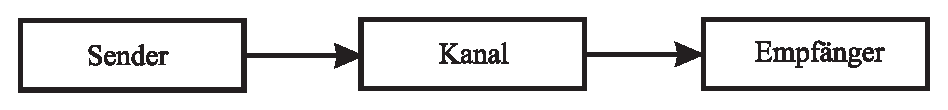
\includegraphics[width = 12cm]{ps/VerallgemeinerteUebertragung.eps}
%\caption{\label{pic:AllgSignalmodell2} Allgemeines Modell für die
%Nachrichtenübertragung.}
%\end{center}
%\end{figure}

\begin{figure}[H]
\begin{center}

\includegraphics[width = 7cm]{ps/AllgSignalmodell}
\caption{\label{pic:AllgSignalmodell} Allgemeines Modell für die
Nachrichtenübertragung.}
\end{center}
\end{figure}


Einige Beispiele für eine solche Übertragung
kennen wir aus unserer täglichen Erfahrung. Wenn wir in einem Gespräch eine
Idee zu unserem Gesprächspartner übertragen wollen, muss zunächst diese Idee in ein
Signal umgewandelt werden, dass über das Medium Luft übertragen werden kann. Beim
Empfänger erfolgt eine hoffentlich fehlerfreie Rückübertragung zum Gehirn.
\begin{figure}[H]
\begin{center}
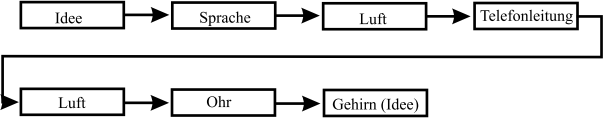
\includegraphics[width = 14cm]{ps/BeispielIdeeIdee}
\caption{\label{pic:BeispielIdeeIdee} Übertragungskette am
Beispiel der Übertragung einer Idee von einer Person zu einer
anderen.}
\end{center}
\end{figure}

Ein weiteres Beispiel ist die Übertragung eines Radioprogramms. Auch hier muss das
eigentlich Nutzssignal zunächst an die Übertragung mittels elektromagnetischer Wellen
angepasst werden.
\begin{figure}[H]
\begin{center}

\includegraphics[width = 7cm]{ps/BeispielRadioLuft}
\caption{\label{pic:BeispielRadio} Übertragungskette am Beispiel
der Rundfunkübertragung.}
\end{center}
\end{figure}

Wir können auch Anwendnungen in unseren Wohnungen finden bei denen sehr komplexe
Übertragungsmechanismen zum Einsatz kommen, \zB das Anhören einer
CD.
\begin{figure}[H]
\begin{center}
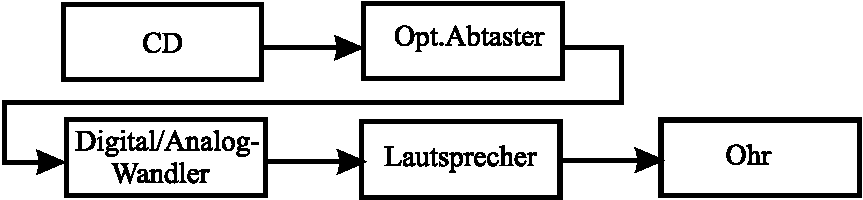
\includegraphics[width = 11cm]{ps/BeispielCDOhr}
\caption{\label{pic:BeispielCDOhr} Übertragungskette am Beispiel
der CD.}
\end{center}
\end{figure}

Aber nicht nur akustische Signale, sondern auch Bilddaten lassen sich in dieses Konzept einpassen,
wie das Beispiel einer Fotoaufnahme zeigt.
\begin{figure}[H]
\begin{center}
\includegraphics[width = 12cm]{ps/BeispielDia}
\caption{\label{pic:BeispielDia} Übertragungskette am Beispiel
eines Landschaftsfotos.}
\end{center}
\end{figure}

Um eine möglichst fehlerfreie Übertragung zu gewährleisten ist es fast immer
notwendig die eigentliche Nachricht zu verändern. Diese
Veränderung kann ganz allgemein als Signalverarbeitung aufgefasst
werde. Da die Signalverarbeitung eine zentrale Aufgabe hat und für
Sie als Studenten von H+A besonders wichtig ist, werden wir uns
zunächst ausschließlich auf die Signalverarbeitung konzentrieren.

\section{Signalverarbeitung}
Die Signalverarbeitung und insbesondere die digitale Signalverarbeitung (DSV) stellt
eine Schlüsseltechnologie für viele moderne Verfahren dar.
Einige Beispiele aus dem Bereich der Telekommunikation und der Sprach- und Audiosignalverarbeitung
sind:
\begin{itemize}
    \item CD-Player
    \item MP3-Player! Gehörbezogene DSV
    \item GSM Mobiltelefon (Handy) (in Zukunft UMTS)
    \item DVD! Visuelle DSV
    \item Synthesizer
\end{itemize}

Das Verständnis der Signalverarbeitung kann insbesondere durch eine einheitliche
Beschreibungssprache erreicht werden, die als Systemtheorie bekannt ist.
Zusätzlich werden nützliche Werkzeuge bereitgestellt, die
eine umfangreiche und in vielen Fällen vollständige
Analyse der Signalverarbeitungsalgorithmen ermöglichen.

\section{Systemtheorie}
Die Systemtheorie ist ein sehr mächtiges Werkzeug zur Beschreibung von SV-Algorithmen.
Gleichzeitig wird die Systemtheorie auch in anderen technischen Bereichen eingesetzt, \zB
in der Automatisierungstechnik. Um die Zusammenhänge etwas zu verdeutlichen, zeigt
Abbildung \ref{pic:SystemtheorieEinordnung} wie die einzelnen Themengebiete
miteinander in Verbindung stehen. Die Systemtheorie ist dabei von so elementarer Bedeutung,
dass zunächst einige Grundbegriffe der Systemtheorie behandelt werden, wie sie für die DSV
benötigt werden.

\begin{figure}[H]
\begin{center}
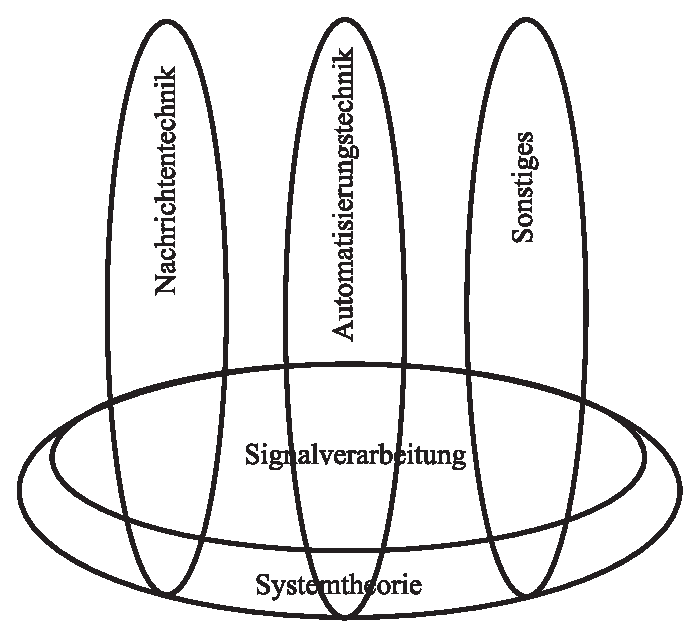
\includegraphics[width = 6cm]{ps/SystemtheorieEinordnung}
\caption{\label{pic:SystemtheorieEinordnung} Zur Einordnung der Systemtheorie.}
\end{center}
\end{figure}

\chapter{Signale}
Zum Verständnis der Signalverarbeitung ist es notwendig eine
mathematische Beschreibung von Signalen zu entwickeln.
Da Signale sehr unterschiedlicher Natur sein können, werden wir zunächst eine grobe
Klassifikation vornehmen.

Um die einzelnen Signalklassen zu entwickeln, betrachten wir
einige Beispiele für natürliche Signale:

\begin{itemize}
    \item Sprache: Für den Studiengang H+A das Signal, das wir am besten
    kennen lernen sollten.
\begin{figure}[H]
\begin{center}
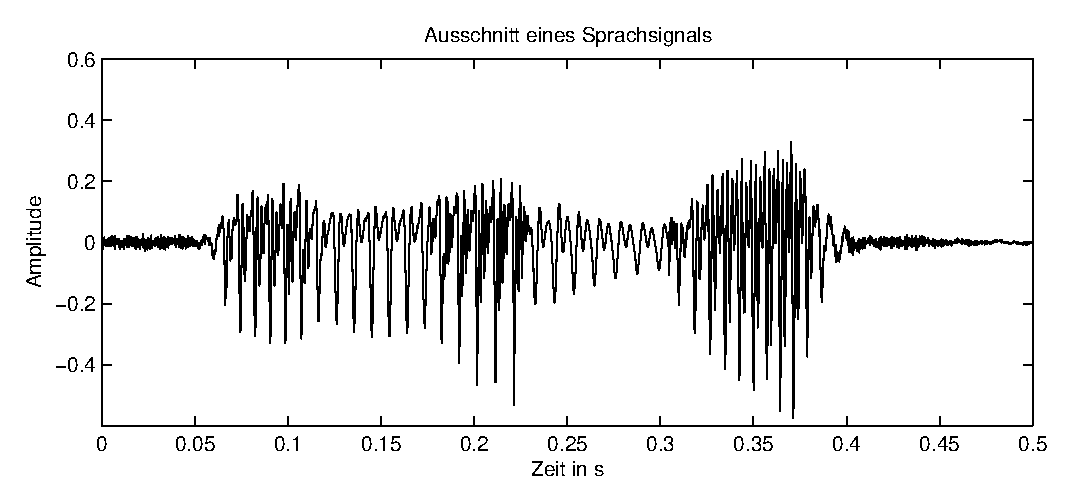
\includegraphics[width = 15cm]{ps/Sprachsignal}
\caption{\label{pic:Sprachsignal} Typischer Amplitidenverlauf über
der Zeit eines Sprachsignals.}
\end{center}
\end{figure}

    \item Musik: Ebenfalls für H+A sehr relevant.
    \item EKG und EEG- Signale (für AT und H+A relevant)
    \item Vitaldaten (Puls, Blutdruck)
    \item Bilder / Videos
    \item Radio- und Fernsehsignale
\end{itemize}

Aber auch aus völlig anderen Bereichen, lasen sich bestimmte
Größen als Signale interpretieren.
\begin{itemize}
    \item DAX-Abschlusskurse
\begin{figure}[H]
\begin{center}
\includegraphics[width = 7cm]{ps/BeispielDaxkurs}
\caption{\label{pic:Daxkurs} Verlauf des DAX bei einer Aktualisierung alle zwei Stunden.}
\end{center}
\end{figure}

    \item Verkehrsampelsignale

\begin{figure}[H]
\begin{center}
\includegraphics[width = 9cm]{ps/Verkehrsampelsignal}
\caption{\label{pic:Verkehrsampel} Ampelsignal im normalen Betrieb.}
\end{center}
\end{figure}

\end{itemize}

Mehr technischer Natur sind \zB
\begin{itemize}
    \item Das optische Signal, dass ein CD-Player von der CD liest
    \item Das Signal, dass ein Pulsmessgerät ausgibt.
    \item Ihr Beispiel
\end{itemize}

Als Gemeinsamkeiten fallen auf, dass die jeweiligen Signale meistens eine
unabhängige Größe beinhalten (meistens die Zeit) und eine abhängige Größe, zum Beispiel
den Schalldruck am Mund. Dies wird mathematisch durch $p(t)$ ausgedrückt\footnote{Aus
der Mathematik ist die Kurzform $y = x^2$ geläufiger als $y(x) = x^2$.}.
Weiterhin ist allen Signalen gemeinsam, dass sie
eine bestimmte Information enthalten.
Deshalb definieren wir:
\wichtig{Signale sind Funktionen oder Wertfolgen, die Informationen repräsentieren}

\section{Klassifikation}
Wir haben gesehen, dass es viele unterschiedliche Signalarten gibt. Die Frage, die sich
stellt ist, ob es Gemeinsamkeiten zwischen verschiedenen Signalen gibt und
wie wir diese Gemeinsamkeiten bezeichnen. Dies kann grob als eine Art Klassifikation der
Signale betrachtet werden.

\subsection{Wertebereich}
Eine erste Unterteilung ist möglich, indem wir den Wertebereich der unterschiedlichen
Signale untersuchen. Es fällt auf, dass ein Teil der Signale keinerlei Grenzen
in der Auflösung haben, so ist bei natürlich gesprochener Sprache, jeder Schalldruck
innerhalb der physikalischen Grenzen
möglich. Im Gegensatz dazu nimmt eine Ampel im Normalbetrieb nur vier Zustände an.

Dies führt zu der Kategorie Wertebereich, die in die beiden Klassen
\wichtig{wertkontinuierlich vs. wertdiskret}
unterteilt werden kann.

\subsection{Definitionsbereich}
Eine weitere sehr wichtige Unterteilung ist der Definitionsbereich. Für Signale
ist dies die Frage der Gültigkeit eines Signals. Beim natürlichen Sprachsignal ist die Gültigkeit
immer gegeben. Ein Gegenbeispiel ist der DAX-Abschlusskurs, der immer nur
um 20.00 Uhr gültig ist.

Somit können wir eine weitere Unterteilung definieren.
\wichtig{zeitkontinuierlich vs. zeitdiskret}

Nur wenn ein Signal in den beiden Kategorien diskret ist, spricht man von einem {\bf digitalen Signal}.

\wichtig{Ein digitales Signal ist wert- und zeitdiskret.}

Abbildung \ref{pic:TabelleWertZeit} zeigt die vier
Kombinationsmöglichkeiten, die sich durch die beiden Kategorien
Wertebereich und Definitionsbereich ergeben.

\begin{figure}[H]
\begin{center}
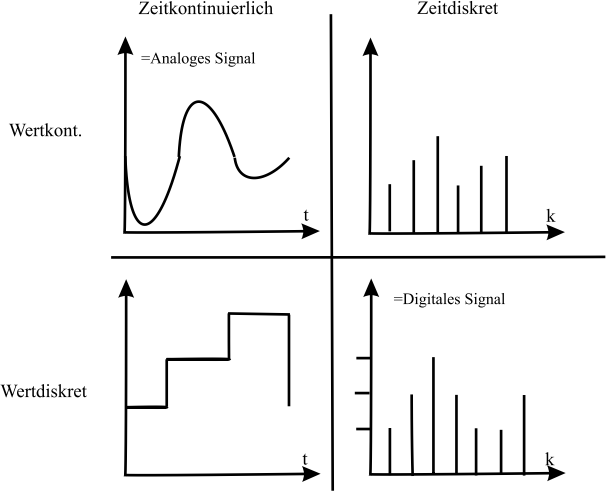
\includegraphics[width = 14cm]{ps/TabelleWertZeit}
\caption{\label{pic:TabelleWertZeit} Die vier
Kombinationsmöglichkeiten für wert- oder zeitkontinuierliche bzw.
wert- oder zeitdiskrete Signale.}
\end{center}
\end{figure}

\subsection{Kanalanzahl}
Betrachtet man die genannten Beispiele, so fällt zumindest bei der CD auf, dass
das Ausgabesignal zweikanalig ist, um die Stereophonie zu erhalten. Andere Signale
sind dagegen einkanalig. Ein weiteres Unterscheidungsmerkmal ist also:

\wichtig{einkanalig vs. mehrkanalig}

Ein besonderer Fall stellen komplexwertige Signale dar, die man als eine besondere
Form der zweikanaligen Signale interpretieren kann, wenn man den Real- und Imaginäranteil
getrennt betrachtet.
\[
    z(t) = x(t) + j\;y(t)
\]
Häufig wird aber auch dieser Aspekt mit zur Klassifikation hinzugezogen.
Somit haben wir ein weiteres Merkmal

\wichtig{reellwertig vs. komplexwertig}

\subsection{Dimensionalität}
Vor der allgemeinen Definition von Signalen wurde von abhängigen und unabhängigen Größen gesprochen.
Nimmt man ein Bild als spezielles Signal bestehen zwischen der x-Achse und der y-Achse
keine Abhängigkeiten. Wir haben somit zwei unabhängige Größen, die ein Signal darstellen.
In diesem Zusammenhang spricht man von Mehrdimensionalität. Die Mehrdimensionalität
wird mathematisch durch die Anzahl der Größen in den Abhängigkeitsklammern ausgedrückt.
Für ein zweidimensionales Bild zum Beispiel durch $B(x,y)$

Unsere Klassifikation lautet also:

\wichtig{eindimensional vs. mehrdimensional}

\subsection{Zufälligkeit}
Betrachtet man die oben angenommenen Beispiele, so ist bei den meisten
Beispielen nicht genau bekannt, wie das Signal aussehen wird. Die
Signale sind in den meisten Fällen näherungsweise zufällig. Man
spricht in diesem Fall auch von stochastischen Signalen.
Im Gegensatz dazu ist das Ampelsignal im normalen Betrieb
absolut vorhersagbar.

Wir haben also ein weiteres Unterscheidungsmerkmal:
\wichtig{stochastisch vs. determiniert}

\subsection{Periodizität}
Bei determinierten Signalen kann eine weitere Unterscheidung vorgenommen werden,
in dem überprüft wird, ob sich das Signal in einem bestimmten Zeitraum $\tau$
regelmäßig wiederholt.
\[
    x(t) = x(t+n\tau) \Mit \quad n\in \mathbb{Z} ,
\]
wobei $\mathbb{Z}$ die Menge der ganzen Zahlen darstellt ($\cdots,-3,-2,-1,0,1,2,3,\cdots$).
Ein Beispiel hierfür ist das Ampelsignal, dass periodisch ist.
Wir unterscheiden also:
\wichtig{periodisch vs. nicht-periodisch}

Alle periodische Signale sind determiniert.

\section{Digitalisierung: eine erste Annäherung}
Wir werden uns im weiteren in erster Linie mit
digitalen Signalen beschäftigen, da die digitale Signalverarbeitung
einen immer größeren Schwerpunkt einnimmt.

Da die meisten natürlichen Signale, insbesondere die für H+A wichtigen Signale, Sprache und
Musik, aber analoge Signale darstellen, müssen diese Signale zunächst digitalisiert werden.
Dazu sind zwei Schritte notwendig. Die Umwandlung zeitkontinuierlicher Signale in zeitdiskrete, sowie
die Umwandlung des unendlich fein aufgelösten Wertebereichs in einen beschränkten diskreten Wertebereich.

Diese beiden Teilaufgaben werden
\begin{itemize}
\item Abtastung ({\em Sampling}) und
\item Quantisierung ({\em Quantization})
\end{itemize}
genannt.

In den nächsten Abschnitten werden zunächst nur pragmatische Betrachtungen gewählt. Die theoretischen
Hintergründe werden später im Abschnitt \ref{sec:Analog} genauer betrachtet.

\subsection{Abtastung \label{sec:Abtastung}}
Bei der Abtastung wird das zeitkontinuierliche Signal in ein zeitdiskretes Signal
umgewandelt. Dies geschieht dadurch, dass aus dem kontinuierlichen Signal
zu bestimmten Zeiten Proben \engl{Samples} entnommen werden. Man kann sich dies
als eine Art Schalter vorstellen, der immer nur für einen kurzen Zeitpunkt das Signal
durchlässt (siehe Abbildung \ref{pic:SignalflussAbtastung})

\begin{figure}[H]
\begin{center}
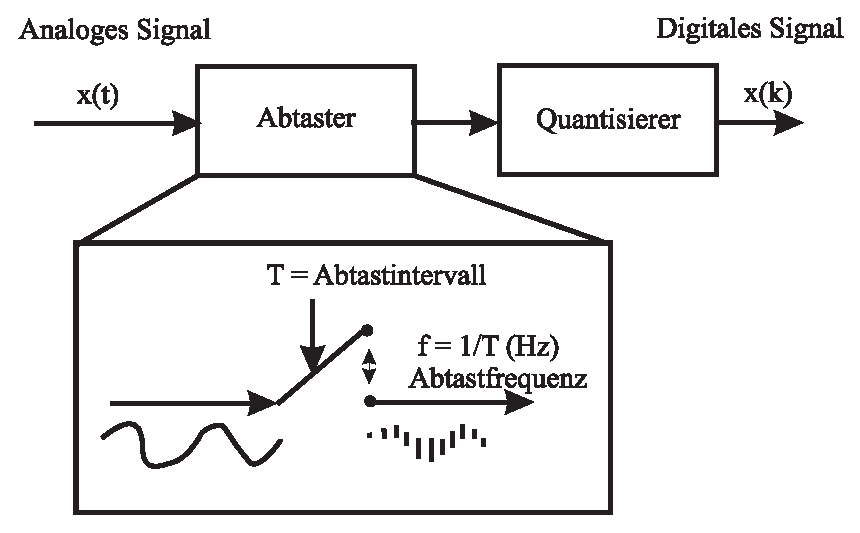
\includegraphics[width = 14cm]{ps/Signalfluss}
\caption{\label{pic:SignalflussAbtastung} Signalfluss zur
Digitalisierung eines analogen Signals.}
\end{center}
\end{figure}


In der DSV geht man in den meisten Fällen implizit davon aus, dass
diese Abtastung in einem regelmäßigen Interval
erfolgt, dass bei Zeitsignalen Abtastinterval $T$ genannt wird
\footnote{Diese Regelmäßigkeit ist aber nicht zwingend, sie vereinfacht nur die weitergehenden Überlegungen.}
(Bei Bildern ist dies die Auflösung).

Die Abtastrate, im weiteren auch mit dem eingedeutschten Begriff Samplingfrequenz $f_s$ bezeichnet,
ist der Kehrwert zum Abtastinterval
\[
    f_s = \frac{1}{T}
\]
und wird in Hertz (Hz) also $1/s$ angegeben.

Die Frage lautet nun, mit welcher Frequenz muss ein Signal abgetastet werden, damit
die digitale Repräsentation dem analogen Original entspricht. Insbesondere,wenn man abschließend
das digitale Signal wieder in ein analoges Signal zurück wandeln will, ist die Frage, welche Frequenz
ist notwendig um eine vollständige Rekonstruktion, also eine verlustlose Diskretisierung,
zu erreichen.

Um dies zu veranschaulichen, sind in der Abbildung \ref{pic:ABtastungErklaerung1}
verschiedene Sinustöne gezeigt, die
bei gleichbleibender Abtastrate abgetastet werden. Es wird deutlich dass, sehr tiefe Frequenzen
besonders gut dargestellt werden (a), je höher die Frequenzen werden, desto weniger Abtastwerte
repräsentieren die analoge Funktion (b,c). Ist die Frequenz des Sinus genau halb so hoch
kann die Funktion gar nicht mehr erkannt werden, da sich eine Konstante ergibt(d).
Erhöht man die Frequenz des Sinus noch weiter entsprechen die Abtastwerte genau den
Abtastwerten einer niedrigeren Frequenz (e,f). Betrachtet man nur die Folge der Abtastwerte
und nicht die Zeitpunkte
des Auftretens\footnote{Diese Information ist nach einer Abtastung nicht mehr vorhanden}, so kommt es
zu Doppeldeutigkeiten. Dieser
Effekt wird {\em Aliasing} genannt.
\begin{figure}[H]
\begin{center}
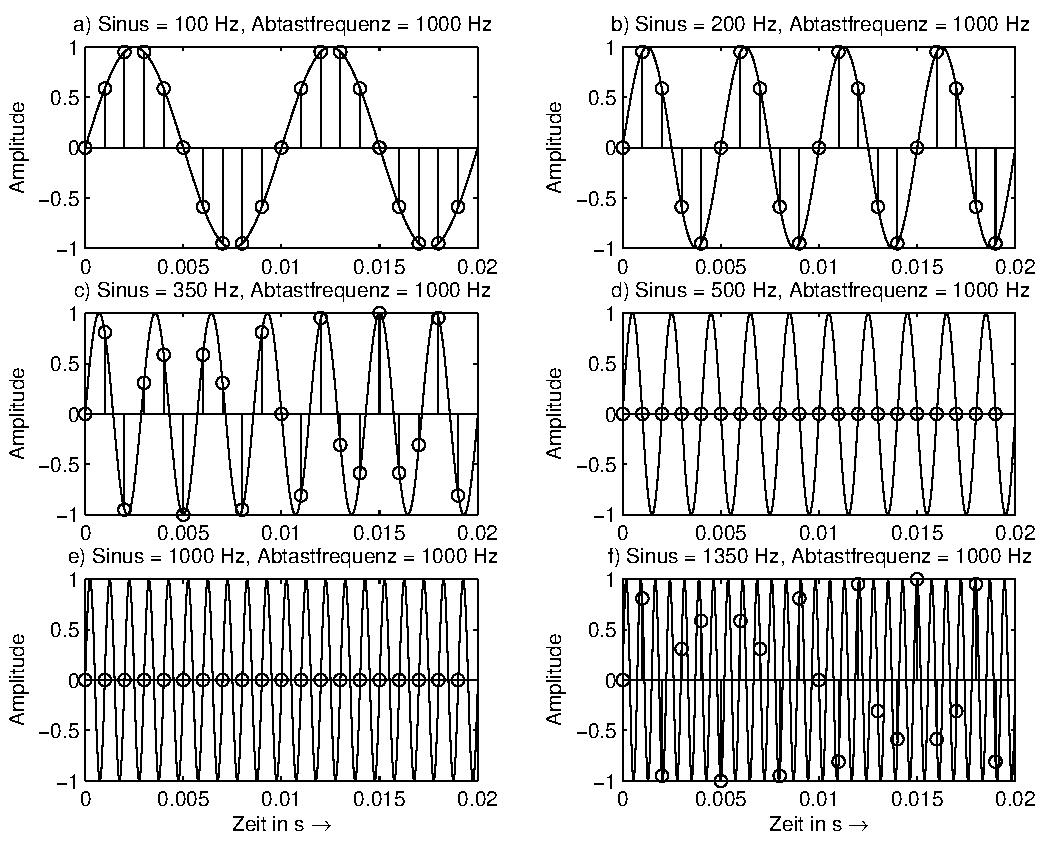
\includegraphics[width = 16cm]{ps/AbtastungErklaerung2}
\caption{\label{pic:ABtastungErklaerung1} Sinusabtastung mit gleichbleibender Abtastrate
für verschiedene Frequenzen.}
\end{center}
\end{figure}

Man kann das Problem aber auch andersherum darstellen. Die Frequenz des Sinus bleibt
gleichbleibend, aber die Abtastrate wird verändert.
Dies ist in Abbildung \ref{pic:ABtastungErklaerung2} gezeigt. Ist die
Abtastrate sehr hoch, kann die Sinusfunktion sehr gut repräsentiert
werden (a). Reduziert man die Abtastfrequenz wird die Anzahl der Samples
die den Sinus repräsentieren immer geringer (b,c). Ist die Abtastfrequenz
genau doppelt so hoch, wie die Frequenz des Sinus, entsteht für diese
Phasenlage ein Nullsignal (d). Es ist also keine Aussage über das Signal mehr möglich.
Erhöht man die Frequenz weiter, so enstehen die schon vorher erwähnten Doppeldeutigkeiten.
\begin{figure}[H]
\begin{center}
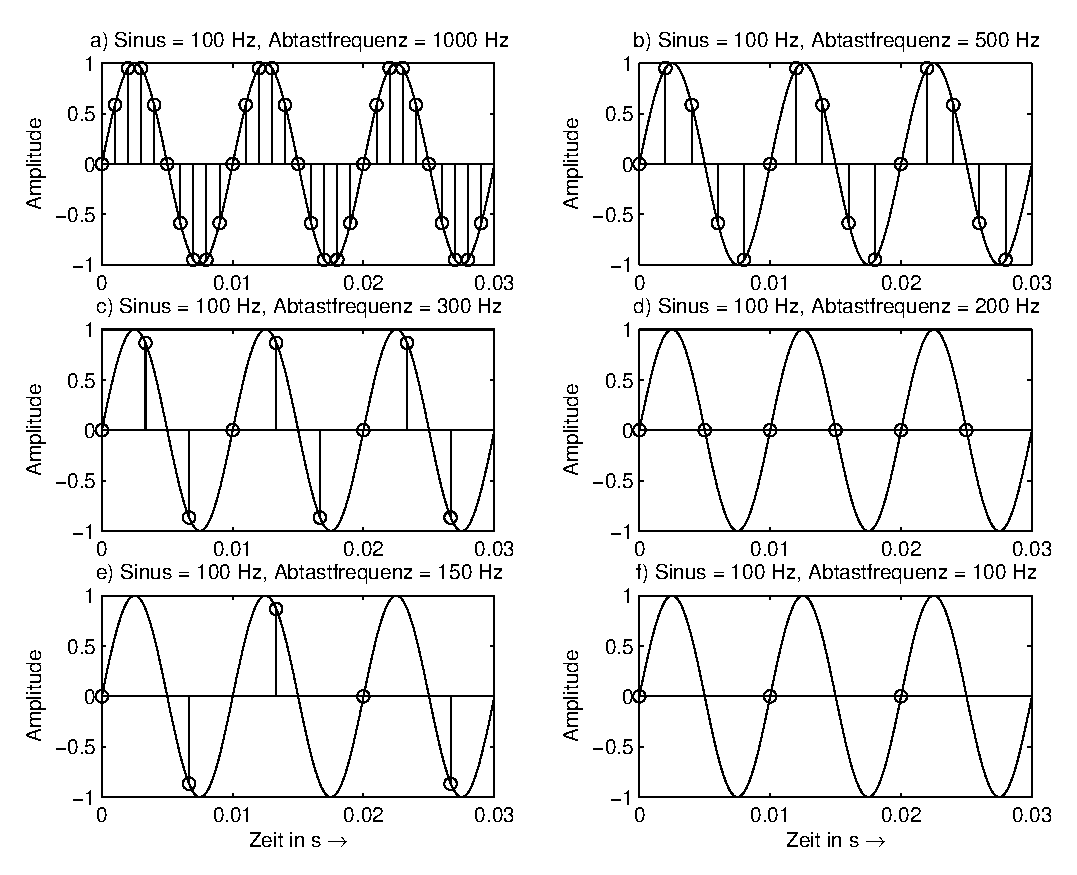
\includegraphics[width = 16cm]{ps/AbtastungErklaerung}
\caption{\label{pic:ABtastungErklaerung2} Sinusabtastung mit unterschiedlichen
Abtastfrequenzen.}
\end{center}
\end{figure}

Um also eine perfekte und eindeutige
Rekonstruktion zu ermöglichen, ist es notwendig, mit wenigstens der doppelten
Frequenz der höchsten im Signal vorkommenden Frequenz abzutasten. Da viele natürliche Signale
keine obere Frequenz haben oder diese so hoch liegt, dass die Abtastung nicht mehr
technisch realisiert werden kann, wird das Eingangssignal einer Abtasteinheit
nach oben begrenzt. Es werden also alle Frequenzen ab einer bestimmten Frequenz aus dem Signal entnommen.
Dieses Prozess bezeichnen wir als Filterung. Das verwendete Filter\footnote{Es heißt
das technische Filter, im Gegensatz zum Kaffeefilter.} wird als Tiefpass-Filter
bezeichnet, da es alle tiefen Frequenzen passieren lässt.

\wichtig{Abtastung ist nur dann eindeutig, wenn das Signal keine Frequenzen enthält, die oberhalb
der halben Abtastfrequenz liegen\footnote{Es wurde bisher nicht gezeigt, dass eine perfekte
Rekonstruktion möglich ist, bzw. dass die wenigen Abtastwerte bei hohen Frequenzen ausreichend sind. Dieser
Tatsache ist hier zunächst zu glauben, da der Beweis nur mit mathematischen Werkzeugen
möglich ist, die zu diesem Zeitpunkt unbekannt sind}
\begin{equation}
f_{max}<\frac{f_s}{2}
\end{equation}
}

Die halbe Samplingfrequenz wird auch als Nyquist-Frequenz bezeichnet.

Um die Abtastung bei einer mathematischen Signalbeschreibung deutlich zu machen, wird
statt der üblichen Beschreibung des analogen  Zeitparameters $t$, die
Index- oder Laufvariable $k$ verwendet\footnote{Lassen Sie sich
nicht verwirren durch andere Bezeichnungen. In der englischsprachigen Literatur wird meist
$n$ als Zeitindex verwendet.}
Eine typisches Zeitsignal $x(t)$ wird also nach der Abtastung zu $x(k)$, wobei
dies eine Abkürzung für $x(kT)$ ist.

\subsection{Quantisierung\label{sec:Quantisierung}}

Der zweite wesentliche Schritt ein digitales Signal zu bekommen ist, die zeitdiskreten Werte
zusätzlich im Wertebereich zu diskretisieren.
Dazu ist es notwendig, eine bestimmte Auflösung und einen bestimmten abzudeckenden Wertebereich festzulegen.
Da wir die Signale digital speichern ist die Auflösung immer in 2er Potenzen angegeben, da
jedes weitere Bit die möglichen Wertestufen um den Faktor 2 erhöht.
Übliche Auflösungen sind 8Bit = 1 Byte, 16Bit = 1 Word oder 32Bit = 1 Long Word.
Damit sind dann 256, 65536 oder $2^{32}$ verschiedene Werte darstellbar.

Zusätzlich muss der Wertebereich nach oben und unten begrenzt sein, da der Wertebereich
von $-\infty  \cdots +\infty$ sonst nicht durch eine begrenzte Anzahl an Stufen aufzulösen ist,
wenn alle Wertestufen den gleichen Abstand haben sollen.

Die eigentliche Werteumwandlung lässt sich am einfachsten anhand von Abbildung
\ref{pic:Quantisierer} zeigen. Auf der x-Achse ist der analoge wertkontinuierliche Eingang
aufgetragen und auf der y-Achse der Ausgang des Diskretisierers, im weiteren Quantisierer
genannt.
\begin{figure}[H]
\begin{center}
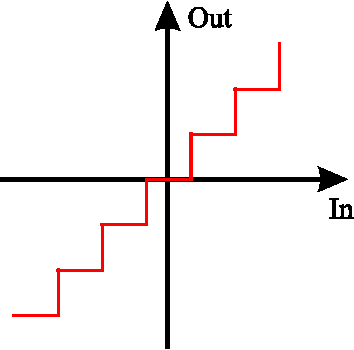
\includegraphics[width = 7cm]{ps/Quantisierer}
\caption{\label{pic:Quantisierer} Einfache Quantisierungskennlinie.}
\end{center}
\end{figure}


Diese stufenförmige Funktion wird Quantisierungskennlinie genannt und kann unterschiedlich
aufgebaut sein. In den meisten Fällen sind die Wertestufen alle gleich hoch, man spricht in diesem
Fall auch von einer linearen Quantisierung\footnote{Wir werden auf den Begriff der Linearität noch
kommen und diesen Begriff an dieser Stelle hinterfragen.} Es gibt aber auch andere
Kennlinie, die eine hohe Auflösung im Bereich um Null und bei großen Eingangswerten
eine geringere Auflösung besitzen (Beispiel siehe Abbildung \ref{pic:NonLinearQuant}).
\begin{figure}[H]
\begin{center}
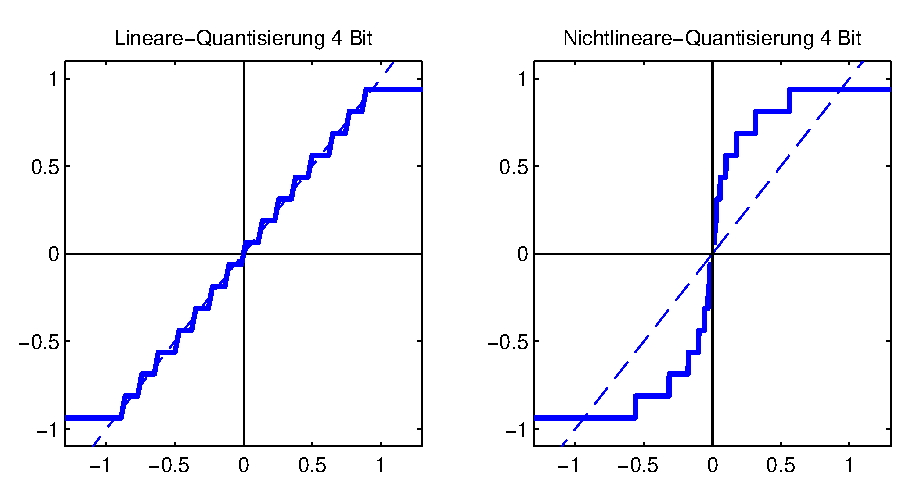
\includegraphics{ps/LogQuant}
\caption{\label{pic:NonLinearQuant} Beispiel einer nicht-linearen
Quantisierungskennlinie.}
\end{center}
\end{figure}

Ein Beispiel hierfür benutzen Sie fast täglich
beim Telefonieren, wo das Signal fast logarithmisch quantisiert wird. Der Vorteil
dieser nicht-gleichförmigen Quantisierung ist die bessere Anpassung an das zu quantisierende
Signal. Als Nachteil erweist sich aber, dass die Signalverarbeitung mit diesen Signalen
sehr viel aufwändiger ist. Deshalb werden diese nicht-gleichförmigen Quantisierer meistens
bei der Speicherung und der Übertragung von Daten verwendet.


Weitere Variationen ergeben sich im Verhalten am Nulldurchgang.
Zum einen kann man das Nullsignal ausschließen oder man weist sehr
kleine Werte alle dem Nullsignal zu (siehe Abbildung
\ref{pic:MidTreadMidRise}). Die letzterer ist die Form die in den
allermeisten Fällen in der Praxis verwendet wird.

\begin{figure}[H]
\begin{center}
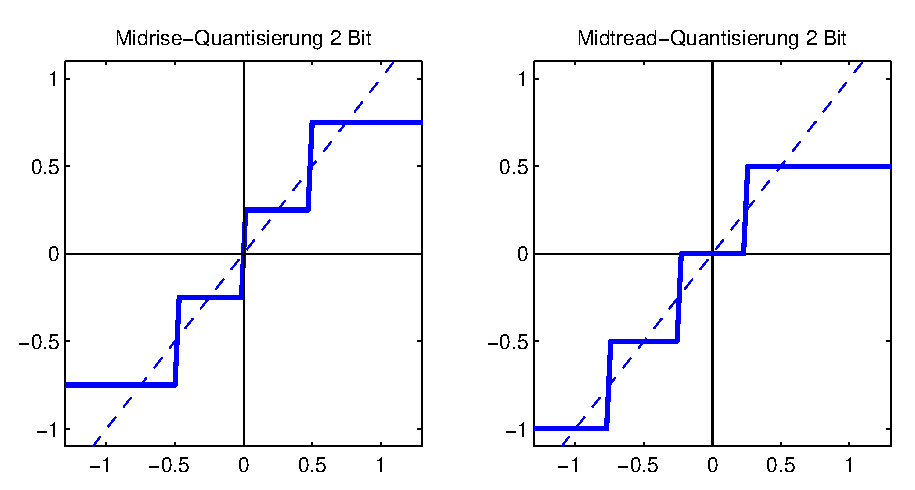
\includegraphics{ps/MidRiseMidTread}
\caption{\label{pic:MidTreadMidRise} Quantisierungskennlinie eines
Mid-Tread und eines Mid-Rise Quantisierers. Üblich ist Mid-Tread.}
\end{center}
\end{figure}


Problematisch ist nun aber, dass die benötigte Auflösung bei einer vollständig symmetrischen
Lösung ungerade sein müsste, da die Null weder eine positive noch eine negative Zahl darstellt.
Gleichzeitig muss aber eine 2er Potenz und somit eine gerade Zahl erreicht werden.
Dies wird gelöst, indem die Null zu den positiven Werten gezählt wird. Aus diesem Grund
ergeben sich am Ausgang der meisten Quantisierer
$2^{Bit-1}$ negative Werte, aber nur $2^{Bit-1}-1$ positive Werte. Diese Werte werden
für die Verarbeitung meist normiert angewendet.
Es ergibt sich dann ein Wertebereich von\footnote{Dieser maximale Wert wird auch als 0dbFS bezeichnet. 0dB,
da der Logarithmus von 1= 0 ist und FS für die englische Bezeichnung Full Scale}.
\[
    -1 \leq x \leq 1-\frac{1}{2^{Bit-1}}
\]

Die Frage, welche Auflösung nötig ist, um eine perfekte Rekonstruktion für einen
bestimmten Wertebereich zu ermöglichen ist aber damit noch nicht beantwortet. Das
Problem ist in Abbildung \ref{pic:QuantisierungSinus}
veranschaulicht, die die Quantisierung einer Sinusfunktion mit wenigen Stufen zeigt.

\begin{figure}[H]
\begin{center}
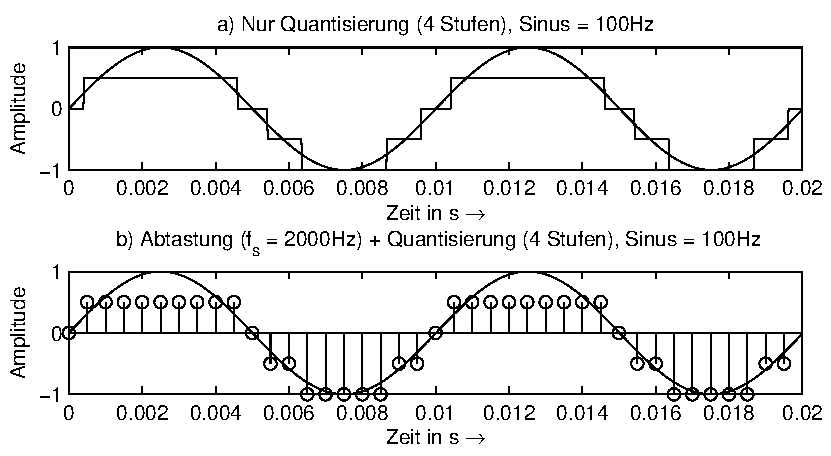
\includegraphics{ps/PlotQuantisierung}
\caption{\label{pic:QuantisierungSinus} Veranschaulichung der Quantisierung
bei einem Sinus als Eingangssignal (Midtread Kennlinie).}
\end{center}
\end{figure}

Es wird deutlich, dass viele unterschiedliche Eingangswerte einem einzigen Ausgangswert
zugewiesen werden (Im Englischen auch als {\em Many--to--One}-Transformation bezeichnet).
Dieser Prozess ist aber immer irreversibel, da aus den quantisierten Werten nicht eindeutig auf die
Originalwerte geschlossen werden kann.

\wichtig{Bei einer Quantisierung kommt es immer zu einem Informationsverlust\footnote{Es kann auch kein Informationsverlust auftreten, wenn das Eingangssignal des Quantisierers auch schon wertdiskret ist.}.}

Die Quantisierung muss also immer so groß gewählt werden, dass sie für den jeweiligen Empfänger angepasst ist. In der Audiologie ist der Empfänger meist das Ohr. Da das Ohr nur einen eingeschränkten Dynamikbereich wahrnimmt, reichen 16Bit, wie sie bei der CD verwendet werden, meistens aus. Die entstandenen Verzerrungen sind für ungeübte Ohren unhörbar und werden als Rauschen wahrgenommen. Dies gilt zumindest wenn die Auflösung bezogen auf die Amplitude des Signals ausreicht.

\section{Einige Elementarsignale}
In der Einführung wurden einige Beispiele für Signale genannt, die meist aus einer direkten Beobachtung der Natur folgten. Für den weiteren Verlauf ist es aber notwendig auf Signale zurückgreifen zu können, die mathematisch beschreibbar sind, um weitere Berechnungen zu ermöglichen

\subsection{Determinierte Signale}
Vollständig beschreibare Signale werden als deterministisch bezeichnet. Ihr
Signalverlauf ist zu jedem Zeitpunkt eindeutig angegeben. Wir unterscheiden
zusätzlich bei den deterministischen Signalen ob eine Periodizität vorliegt, oder nicht.
\subsubsection{Periodische Signale}
Periodische Signale zeichnen sich durch eine Wiederholung ihrer Signalform
innerhalb eines bestimmten Periodendauer $P$ aus. Es gilt:
\begin{equation}\label{eq:PeriodischSignale}
    x(t) = x(t+nP) \quad \Mit \quad n\in\mathbb{Z}
\end{equation}
Einige periodische Signale sind:
\begin{itemize}
\item{{\bf Sinus:}
Die vollständige Beschreibung des Sinustones ist durch
\begin{equation}
y(t) = \underbrace{a}_{\mbox{Amplitude}} \sin(\underbrace{\omega}_{\mbox{Kreisfrequenz}} t +
\underbrace{\varphi}_{\mbox{Phase}})
\end{equation}
bzw. häufiger durch
\begin{equation}
y(t) = \underbrace{a}_{\mbox{Amplitude}} \cos(\underbrace{\omega}_{\mbox{Kreisfrequenz}} t +
\underbrace{\varphi}_{\mbox{Phase}})
\end{equation}
gegeben\footnote{Der Cosinus ist für viele Anwendungen leichter zu berechnen, \zB bei der Fourier-Transformation, da sich ein rein reelles Spektrum ergibt.}. Die Kreisfrequenz $\omega$ setzt sich dabei aus $\omega =
2 \pi f$ zusammen, wobei $f$ die eigentliche Frequenz in Hertz
$1Hz = 1 s^{-1}$ darstellt. Sie gibt an, wie viele Perioden einer
Schwingung in einer Sekunde Signal vorhanden sind, daher $s^{-1}$
= pro Sekunde als Maßeinheit.
Um die anderen Parameter etwas zu verdeutlichen, sind in den Abbildungen \ref{pic:SinusAmplitude}
- \ref{pic:SinusPhase} verschiedene Sinustöne bei variierenden Parametern gezeigt.
\begin{figure}[htb]
\begin{minipage}{5cm}
%\begin{figure}[htb]
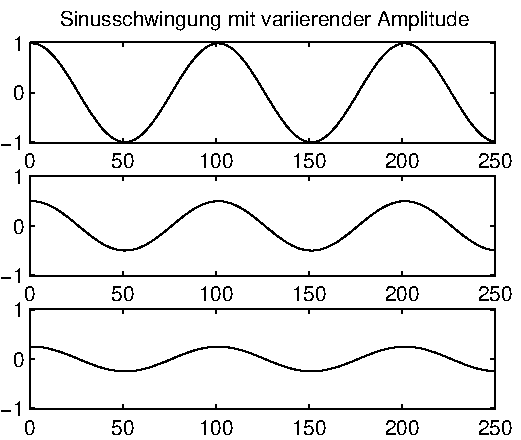
\includegraphics [width = 5cm]{ps/SinusAmplitude}
\caption{\label{pic:SinusAmplitude} Veränderung der Amplitude}
%\end{figure}
\end{minipage}
\begin{minipage}{5cm}
%\begin{figure}[htb]
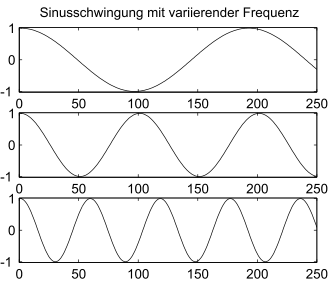
\includegraphics [width = 5cm]{ps/SinusFrequenz}
\caption{\label{pic:Veranschaulichung Schwingung}Veränderung der Frequenz}
%\end{figure}
\end{minipage}
\begin{minipage}{5cm}
%\begin{figure}[htb]
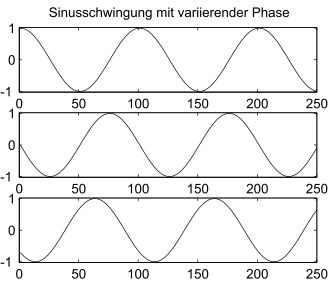
\includegraphics [width = 5cm]{ps/SinusPhase}
\caption{\label{pic:SinusPhase}Veränderung der Anfangsphase}
%\end{figure}
\end{minipage}
\end{figure}
}

Die Erzeugung einer diskreten Folge, die einen Cosinus repräsentiert kann durch
\begin{equation}\label{eq:DiscreteSinus}
    y(k) = a \cos\left(2\pi k \frac{f_0}{f_s}  + \varphi_0 \right)
\end{equation}
erzeugt werden. Bei dieser Darstellung ist die Abkürzung für
\[
    kT = \frac{k}{f_s}
\]
leicht erkennbar \footnote{Üblicherweise wird die Cosinus-Fkt als Elemetarsignal genutzt und nicht der Sinus, da dieser für spätere Betrachtungen einige positive Eigenschaften aufweist}.


\item{{\bf Dreieck:} Ein periodisches Dreieckssignal zu beschreiben, kann auf zwei Arten erfolgen.
Eine sehr einfache Beschreibung erfolgt über eine abschnittsweise Definition. Eine Periode der
Dreiecksschwingung ist gegeben durch
\begin{equation}\label{eq:DreieckAbschnitt}
x_{1D}(t) = \bigg\{ \begin{array}{lcc}
1-\left|\frac{2t}{L}\right| & & -L \leq t \leq L\\
0 & & \mbox{sonst}
\end{array}
\end{equation}
Die Periodizität wird abschließend durch
\begin{equation}
x(t+n2L) = x(t)
\end{equation}
für $n \in\mathbb{Z}$ erzeugt.
\begin{figure}[h]
\begin{center}
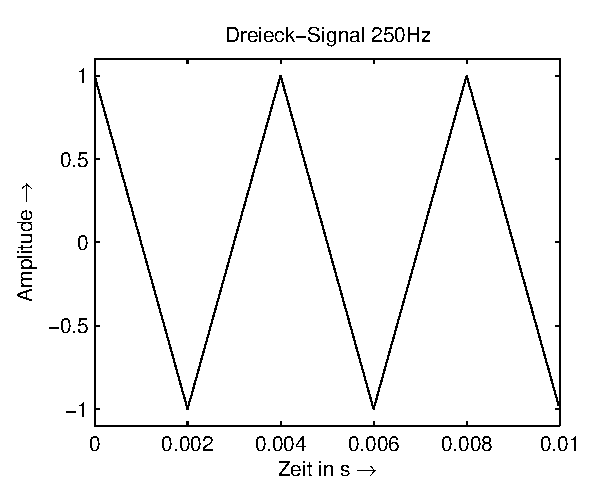
\includegraphics[width = 8cm]{ps/Dreieck}
\caption{\label{pic:DreieckFunktion} Ausschnitt eines Dreiecksignals.}
\end{center}
\end{figure}

Eine weitere Möglichkeit periodische Signale auszudrücken, ergibt sich aus dem Fourier-Theorem. Es besagt,
dass sich alle periodischen Signale auf eine Summe von Sinussignalen zurückführen lassen. Die zerlegten
komplexen Signale lassen sich dann durch eine sog. Fourier-Reihe beschreiben.
Für das Dreieckssignal ist diese Fourier-Reihe durch
\begin{equation}\label{eq:DreieckFourier}
y(t) = \frac{8}{\pi^2}\left(\sin(\omega t) - \frac{1}{3^2} \sin(3\omega t) + \frac{1}{5^2} \sin(5 \omega t) - \cdots\right)
\end{equation} 
oder
\begin{equation}\label{eq:DreieckFourier2}
y(t) = \frac{8}{\pi^2}\left(\cos(\omega t) + \frac{1}{3^2} \cos(3\omega t) + \frac{1}{5^2} \cos(5 \omega t) + \cdots\right)
\end{equation} 
gegeben. Hierbei handelt es sich also um eine unendliche Reihe von Sinustönen, die nur ungeradzahlige
Vielfache der Grundfrequenz\footnote{Treten in einer komplexen Schwingung ganzzahlige (ob
geradzahlig oder ungeradzahlig ist nicht relevant) Vielfache der Grundfrequenz auf, so werden diese
Vielfachen auch Harmonische der Grundfrequenz genannt. Die erste Harmonische ist dabei die Grundfrequenz
selbst.} sind, wobei die Amplitude mit dem Quadrat des Vielfachen abnimmt. Für eine digitale Realisierung
stellt sich hier nun ein Problem ein. Würden wir die abschnittsweise Definition aus
Gleichung \ref{eq:DreieckAbschnitt} direkt in einem digitalen System implementieren, so würde dieses
Signal nach Gleichung \ref{eq:DreieckFourier} auch Frequenzen oberhalb der halben Abtastfrequenz
aufweisen. Ein so direkt erzeugtes Dreieckssignal besitzt deshalb immer Aliasing-Anteile, die aber
in einigen Fällen durch die sehr geringe Amplitude vernachlässigbar sind.
\tbd{Diskrete Dreieck Schwingung}
}
\item{
{\bf Rechteck:} Für das Rechtecksignal funktionieren ebenfalls die beiden Methoden.
Wir können eine abschnittsweise Definition verwenden:
\begin{equation}\label{eq:RechteckAbschnitt}
x_{1R}(t) = \bigg\{ \begin{array}{lcc}
-1 & & -L \leq t < 0\\
1 & &0 \leq t < L
\end{array}
\end{equation}
Die Periodizität wird wieder durch
\begin{equation}\label{eq:Periodizitaet}
x(t+n2L) = x_{1R}(t)
\end{equation}
für $n \in \mathbb{Z}$ erreicht.

Die Fourier-Reihe für ein periodisches Rechtecksignal ist
\begin{equation}\label{eq:RechteckFourier}
y(t) = \frac{4}{\pi}\left(\sin(\omega t) + \frac{1}{3} \sin(3\omega t) + \frac{1}{5} \sin(5 \omega t) + \cdots\right).
\end{equation}
Auch hier treten nur ungeradzahlige Harmonische auf, die aber im Vergleich zu der Dreiecksschwingung
nur mit dem Vielfachen und nicht mit dem Quadrat abnehmen. Dies bedeutet, dass die Aliasing-Problematik
noch ausgeprägter ist.

Eine dritte Methode, die eine besonders einfache Implementierung ermöglicht, ergibt sich aus
der signum-Funktion, die jeweils das Vorzeichen angibt.
\begin{equation}
sign(x) = \left\{ \begin{array}{lcc}
-1 & & x<0\\
0 & & 0\\
1 & & x>0
\end{array} \right.
\end{equation}
Eine Rechteckfunktion kann nun sehr einfach durch das Vorzeichen der Sinusfunktion angegeben werden:
\begin{equation}\label{eq:EasyRechteck}
x(t) = sign(\sin(\omega t));
\end{equation}
bzw. in diskreter Form durch
\begin{equation}\label{eq:EasyRechteckDiskret}
x(k) = sign(\sin\left(2\pi k \frac{f_0}{f_s}\right));
\end{equation}

\begin{figure}[h]
\begin{center}
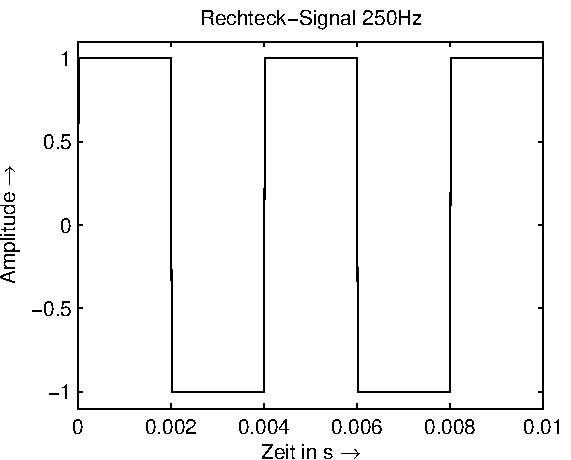
\includegraphics[width = 8cm]{ps/Rechteck}
\caption{\label{pic:RechteckFunktion} Ausschnitt eines Rechtecksignals, erzeugt mit \ref{eq:EasyRechteck}.}
\end{center}
\end{figure}



}
\item{
{\bf Sägezahn:} Eine weitere etwas speziellere Schwingung stellt die Sägezahnschwingung dar, die
besonders häufig bei Synthesizern als Quellensignal zur Erzeugung von Tönen verwendet wird.
Es sind wieder zwei Definitionen möglich.
Die abschnittsweise Definition ergibt sich zu
\begin{equation}
x(t) =\bigg\{ \begin{array}{lcc}
-1+ t/L & &  0 \leq t < 2L\\
0 & & \mbox{sonst}
\end{array}
\end{equation}
Die Periode wird erneut durch Gleichung \ref{eq:Periodizitaet} erzeugt.
Interessant ist die Fourier-Reihenentwicklung:
\begin{equation}
y(t) = \frac{2}{\pi}\left(\sin(\omega t) - \frac{1}{2} \sin(2\omega t) + \frac{1}{3} \sin(3\omega t)
- \frac{1}{4} \sin(4\omega t) + \frac{1}{5} \sin(5 \omega t) - \cdots\right).
\end{equation}
Bei der Sägezahnschwingung treten alle ganzzahligen Harmonischen auf und der Abfall der Amplitude ist gering.
Dieser hohe Anteil an Harmonischen ist auch die Begründung
für den Einsatz bei der elektronischen Klangerzeugung, da sich ein vollerer Klang ergibt, der anschließend manipuliert werden kann.
\begin{figure}[h]
\begin{center}
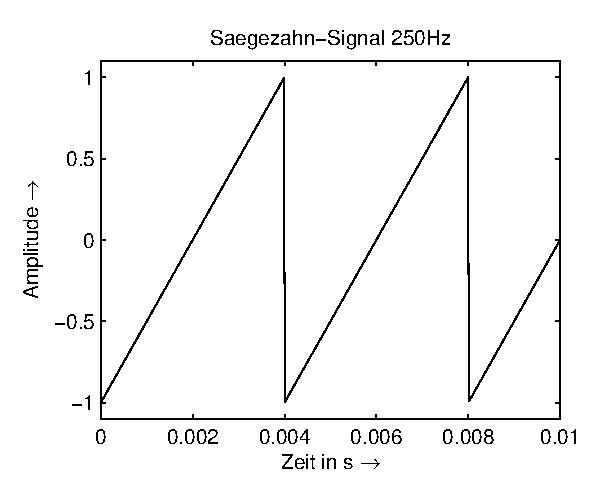
\includegraphics[width = 8cm]{ps/Saegezahn}
\caption{\label{pic:SaegezahnFunktion} Ausschnitt eines Sägezahnsignals.}
\end{center}
\end{figure}
\tbd{Diskreter Sägezahn}
}
\end{itemize}

\subsubsection{Impulssignale}
Eine weitere wichtige Klasse der determinierten Signale stellen die Impulssignale dar:
\begin{itemize}
    \item{{\bf Delta-Impuls\footnote{Auch als zeitdiskreter Dirac-Impuls bekannt}:}
    Der Delta-Impuls ist die wichtigste digitale Impulsfolge, sie wird auch
    als Kronecker-Delta bezeichnet und ist definiert durch
    \begin{equation}
    \delta(k) = \bigg\{ \begin{array}{lcc}
       1 & & k = 0\\
        0  & & \mbox{sonst}
    \end{array}
    \end{equation}
    Aus der Definition folgt
    \begin{equation}
        x(k) \delta(k) = x(0),
    \end{equation}
    was als Siebeigenschaft des Delta-Impulses bekannt ist.
\begin{figure}[h]
\begin{center}
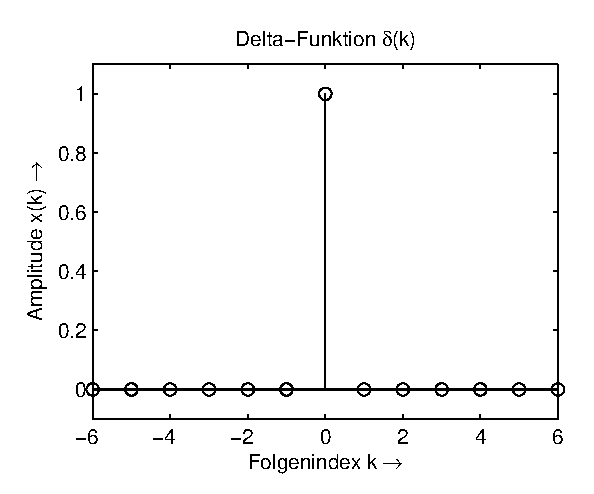
\includegraphics[width = 8cm]{ps/DeltaFunktion}
\caption{\label{pic:DeltaFunktion} Delta-Folge.}
\end{center}
\end{figure}

}
\item{{\bf Sprungfolge:} Die Sprungfolge ist neben dem Delta-Impuls eine weitere sehr wichtige
    Folge zur Beurteilung digitaler Systeme.
    \begin{equation}\label{eq:Def:Sprungfolge}
        \gamma(k) = \bigg\{ \begin{array}{lcc}
        1 & & k \geq 0\\
        0 & & \mbox{sonst}
        \end{array}
    \end{equation}
\begin{figure}[h]
\begin{center}
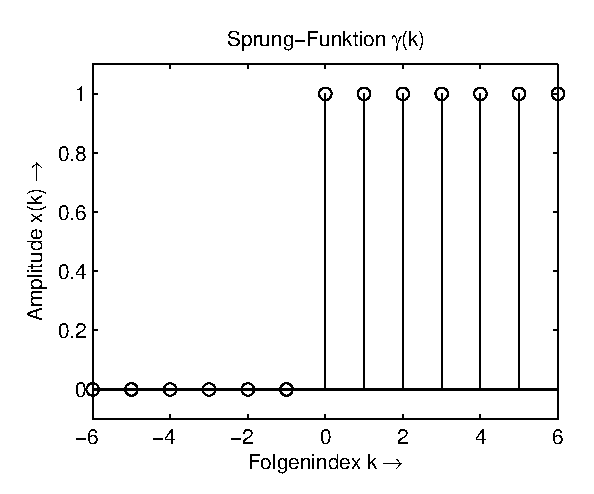
\includegraphics[width = 8cm]{ps/SprungFunktion}
\caption{\label{pic:SprungFunktion} Sprung-Folge.}
\end{center}
\end{figure}
}
\item{{\bf Exponential Impuls:} Die Exponentialfolge ist durch
    \begin{equation}
        x(t) = A e^{\alpha t}
    \end{equation}
    gegeben, wobei $\alpha$ die Dämpfungskonstante angibt und nur für $\alpha < 1$ eine stabile Funktion darstellt.
    Häufig wird aber statt $\alpha$ direkt anzugeben eine sog. Zeitkonstante $\tau = -1 / \alpha$ angegeben.
    Diese beschreibt die Zeit, in der die Funktion auf ca. $37$\% von $A$ abgeklungen ist (siehe
    Abbildung \ref{pic:ExpImpulse}) und das Integral der Exponentialfunktion dem äquivalenten Rechteck bis $\tau$ entspricht.
    \begin{figure}[h]
    \begin{center}
    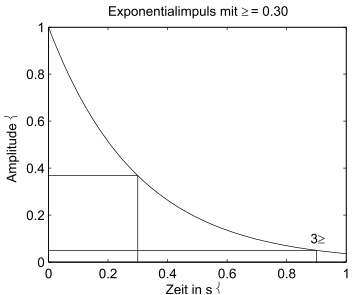
\includegraphics[width = 8cm]{ps/ExpImpulse}
    \caption{\label{pic:ExpImpulse} Exponential Impuls für $\tau = 0.3$s. Eingezeichnet ist
    zusätzlich der $\approx 5$\% Punkt, der sich bei $3\tau$ ergibt.}
    \end{center}
    \end{figure}
    
    
    In der diskreten Form ist die Wertefolge durch

    \begin{equation}\label{eq:ExpImpulseDiskret}
        x(k) = A e^{\alpha k/f_s}
    \end{equation}
    gegeben. Abbildung \ref{pic:ExpImpulseDiskret} zeigt einen diskreten Exponentialimpuls mit
    den Parametern $A = 1, f_s = 2$kHz und $\tau = 3$ms.

    \begin{figure}[h]
    \begin{center}
    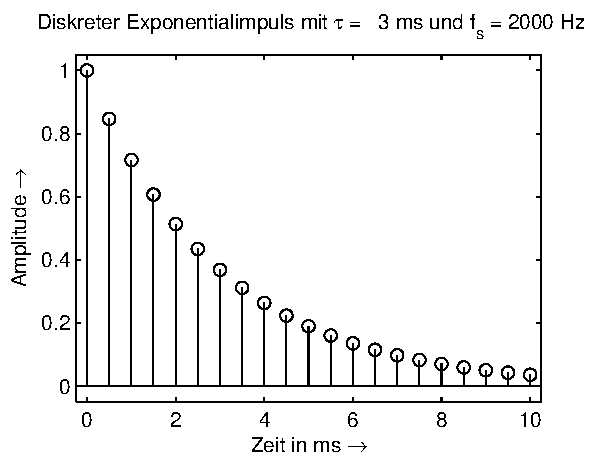
\includegraphics[width = 8cm]{ps/ExpImpulseDiskret}
    \caption{\label{pic:ExpImpulseDiskret} Diskreter Exponential Impuls für
    $\tau = 3$ms.}
    \end{center}
    \end{figure}
    
    Eine alternative Beschreibung ist die Definition als Exponentialfolge
    \[
        x(k) = \alpha_2^{k} \gamma(k)
    \]
    mit
    \[
        \alpha_2 = 1-\frac{1}{\tau f_s}
    \]
    
    }
    \item{{\bf si-Signal:} Die si-Funktion ist zunächst analog definiert und wird in
    nachfolgenden Abschnitten
    benötigt, um \zB die Abtastung genauer zu erläutern.
    \begin{equation}
    si(t) = \frac{\sin t}{t}
    \end{equation}
    bzw.\ häufig wird auch
   \begin{equation}
    sinc(t) = \frac{\sin \pi t}{\pi t}
    \end{equation}
    definiert. In Matlab ist nur \verb/sinc/ implementiert.
    Der Impuls ist in beiden Fällen eine abklingende Sinusschwingung. Der Unterschied ist die
    x-Achsen-Skalierung.
    \begin{figure}[H]
    \begin{center}
    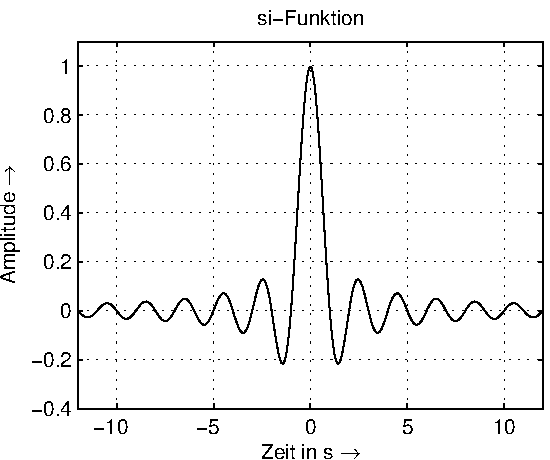
\includegraphics[width = 8cm]{ps/SiFunktion}
    \caption{\label{pic:SiFunktion} Sinc-Impuls auf den Definitionsbereich $-12 \leq t \leq 12$ beschränkt.}
    \end{center}
    \end{figure}
    Für die diskrete si-Folge, nutzen wir die Definition des diskreten Sinus
    aus Gleichung \ref{eq:DiscreteSinus}, mit der Amplitude 1 und einem Anfangswinkel von $\pi/2$.
    Somit wird die Cosinus-Funktion zum Sinus. Es ergibt sich also für die diskrete si-Folge
    \begin{equation}\label{eq:DEF:DiscreteSi}
        si(k) = \frac{sin \left(2\pi k\frac{f_0}{f_s} \right)}{2\pi k\frac{f_0}{f_s}}
    \end{equation}
    Abbildung \ref{pic:SiFunktionDiskret} zeigt eine diskrete si-Folge. Die 100Hz Schwingung
    bei einer Abtastrate von $f_s = 1000$ Hz ist gut an den Nulldurchgängen zu erkennen.
    \begin{figure}[H]
    \begin{center}
    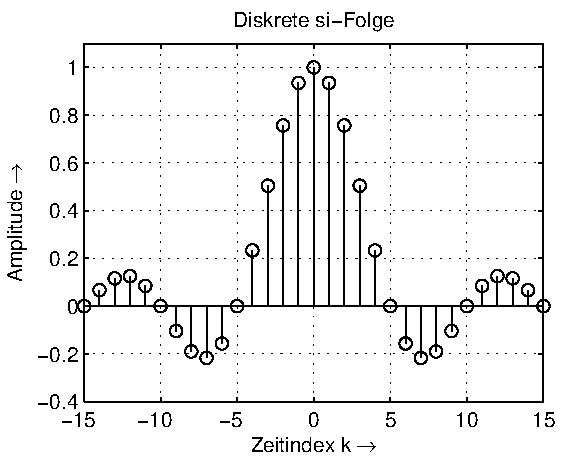
\includegraphics[width = 8cm]{ps/SiFunktionDiskret}
    \caption{\label{pic:SiFunktionDiskret} Si-Folge im Bereich $-15 \leq k \leq 15$ für $f_0 = 100$ Hz und
    $f_s = 1000$ Hz.}
    \end{center}
    \end{figure}

    }
    \item{{\bf Dirac-Impuls:} Der analoge Dirac-Impuls $\Dirac{t}$,
kann nicht direkt als Funktion definiert werden. Statt dessen
erfolgt die Definition über das Integral
\begin{equation}\label{eq:Def:Dirac-Impulse}
   \int\limits_{-\infty}^{\infty}f(t)\Dirac{t} dt = f(0),
\end{equation}
wobei $f(t)$ eine beliebige stetige und differenzierbare Funktion
ist. Die Aussage der Gleichung \ref{eq:Def:Dirac-Impulse} ist, dass der Dirac-Impulse aus
einem Signal nur und ausschließlich den Wert des Signals zum
Zeitpunkt Null herausfiltert. Dies wird auch als Sieb-Eigenschaft
bezeichnet und entspricht der besonderen Eigenschaft des
Delta-Impulses für diskrete Signale. Da keine direkte Definition
möglich ist, spricht man beim Dirac-Impulse von einer
verallgemeinerten Funktion. Diese besondere Klasse ist auch unter
dem Begriff Distributionen bekannt. Durch die Definition als unendlich kurzen
und unendlichen hohen Impuls wird deutlich, dass dieser Impuls nicht
realisierbar ist, sondern eine reine theoretische Konstruktion darstellt, die
sich aber als sehr nützlich Werkzeug zum Berechnen bestimmter Probleme heraus gestellt hat.

Weitere Eigenschaften des Dirac-Impulses sind:
\begin{equation}\label{eq:Eigenschaft1:Dirac}
    \Dirac{t} = 0 \fuer t \neq 0
\end{equation}
Außerdem gilt
\begin{equation}\label{eq:Eigenschaft2:Dirac}
     \int\limits_{-\infty}^{\infty}\Dirac{t} dt = 1
\end{equation}
Aus der Definition und den beiden Eigenschaften können weitere
wichtige Eigenschaften abgeleitet werden. So gilt für den zeitlich
verschobenen Dirac-Impuls:
\begin{equation}\label{eq:Eigenschaft3:Dirac}
    x(t)\Dirac{t-t_0} = x(t_0)\Dirac{t-t_0}
\end{equation}
und
\begin{equation}\label{eq:Eigenschaft4:Dirac}
   \int\limits_{-\infty}^{\infty}x(t)\Dirac{t-t_0} dt = x(t_0),
\end{equation}
Für einen zeitlich skalierten Dirac-Impuls gilt:
\begin{equation}\label{eq:EigenschaftSkalierung:Dirac}
    \Dirac{\alpha t} = \frac{1}{|\alpha|}\Dirac{t} \quad
    \mbox{bzw.}\quad \int\limits_{-\infty}^{\infty}\Dirac{\alpha t} dt =
    \frac{1}{|\alpha|}
\end{equation}
    }
\end{itemize}

\subsection{stochastische Signale \label{sec:stochastEinfuehrung}}
Eine sehr wichtige Klasse an Signalen sind die stochastischen oder
auch rauschförmigen Signale. Sie zeichnen sich dadurch aus, dass
man den Signalverlauf nicht direkt vorhersagen kann. Trotzdem
ist es möglich bestimmte Eigenschaften rauschförmiger Signale
zu beschreiben. Einige grundlegende Beschreibungsgrößen sind:

\begin{itemize}
\item{{\bf Mittelwert:} Die Schätzung\footnote{Schätzungen werden häufig durch $\hat{\cdot}$ markiert}
des Mittelwert ist definiert als die Summe aller
Werte geteilt durch die Anzahl $N$ der gemittelten Werte
\begin{equation}
    \hat{\mu} = \bar{x} = \frac{1}{N} \sum_{k = 1}^{N} x(k)
\end{equation}
}
\item{{\bf Varianz:} Die Schätzung der Varianz ist die mittlere quadratische Abweichung aller Werte vom Mittelwert.
Die Wurzel aus der Varianz wird Standardabweichung $\sigma$ genannt. Deshalb definieren wir die
Varianz durch $\sigma^2$
\begin{equation}
    \hat{\sigma}^2 = \frac{1}{N-1} \sum_{k = 1}^{N} (x(k)-\mu)^2
\end{equation}
}

\item{{\bf Amplitudenverteilung:} Die Amplitudenverteilung gibt an, wie oft die einzelne Amplitudenwerte
im Signal vorkommen. Dies kann häufig mathematisch ausgedrückt werden. Liegt eine
bestimmte Datenfolge vor, wird statt dessen das Histogramm berechnet. Das Histogramm unterteilt den
Eingangsbereich der Amplituden in gleichbleibende Abschnitte und zählt dann aus, wie oft
die Datenfolge Werte in diesem Bereich hat. In Matlab wird dies durch den Befehl \Matlab{hist}
realisiert. Zwei sehr oft vorkommende Amplitudenverteilungen bei Rauschsignalen sind die
gleichförmige Verteilung und die gaussförmige Verteilung. Bei der gleichförmigen Verteilung
kommen in einem definierten Wertebereich alle Amplitudenwerte gleich oft vor. In Matlab
werden Rauschsignale mit dieser Eigenschaft durch den Befehl \Matlab{rand} erzeugt.
Die Verteilung bei der Gauss-Verteilung hat dagegen eine Glockenform. Bestimmte Wertebereiche kommen
also häufiger vor als andere. Die Beschreibung ist mathematisch durch
\begin{equation}
 p(x) = \frac{1}{\sigma \sqrt{2\pi}} e^{-\frac{(x(k)-\mu)^2}{2\sigma^2}}
\end{equation}
gegeben. Wir sehen, dass die beiden Größen Mittelwert und Varianz hier als formgebende Größen
verwendet werden. In Matlab können solche Verteilungen mit dem Befehl \Matlab{normrnd} erzeugt werden.
Gaussverteiltes Rauschen mit der Varianz $\sigma^2= 1$ und dem Mittelvert $\mu= 0$ erzeugt der
Befehl \Matlab{randn}.
Abbildung \ref{pic:Verteilungen} zeigt einige Beispiele mit unterschiedlichen Parametern.
\begin{figure}[H]
\begin{center}
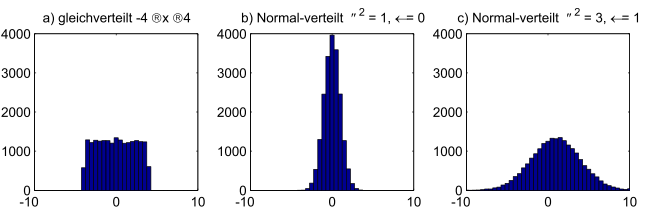
\includegraphics[width = 16cm]{ps/Verteilungen}
\caption{\label{pic:Verteilungen} Beispiele für unterschiedliche Amplitudenverteilungen, wobei
für alle drei Bilder 20000 Datenwerte verwendet wurden.}
\end{center}
\end{figure}
Die Gauss-Verteilung wird auch als Normal-Verteilung bezeichnet. Sie hat eine
große Bedeutung, da bei einer unendlichen Mittelung vieler unabhängiger, gleichverteilter
Verteilungen immer eine Normal-Verteilung am Ende herauskommt. Diese Tatsache wird
zentraler Grenzwertsatz genannt.
}
\end{itemize}

\section{Weitere Eigenschaften von Signalen}
\subsection{Kausalität}
Kausalität bedeutet, dass eine Wirkung immer eine zeitlich vorhergehende Ursache haben muss.
Für Signale heißt diese Eigenschaft, dass keine Signalanteile vor $t = 0$ existieren dürfen.
Alle Anteile mit $t<0$ oder $k < 0$ sind nicht-kausale Anteile des Signals (siehe Abbildung
\ref{pic:KausalErklaerung}).

\begin{figure}[h]
\begin{center}
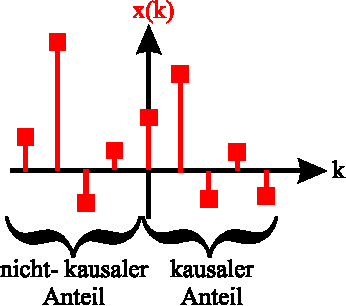
\includegraphics{ps/KausalErklaerung}
\caption{\label{pic:KausalErklaerung} Erklärung zum Begriff der Kausalität bei Signalen.}
\end{center}
\end{figure}

\subsection{Energie und Leistung \label{sec:EnergUndLeistung}}
Es muss zwischen Energie- und Leistungssignalen unterschieden werden
\begin{itemize}
\item{Die Energie eines diskreten Signals ist durch
\begin{equation}
    E_x = \sum_{k = -\infty}^{\infty} |x(k)|^2
\end{equation}
gegeben. Aufgrund dieser Definition ist deutlich, dass alle periodischen Signale
eine Energie $E_x=\infty$ haben.

Für analoge Signale gilt:
\begin{equation}
    E_x = \int_{-\infty}^{\infty} |x(t)|^2 dt
\end{equation}
}
\item{Die Definition der mittleren Leistung wird im diskreten Fall durch
\begin{equation}
    P_x =\lim_{n\rightarrow \infty} \frac{1}{2n+1} \sum_{k = -n}^{n} |x(k)|^2
\end{equation}
und für analoge Signale durch
\begin{equation}
    P_x =\lim_{T\rightarrow \infty} \frac{1}{T} \int_{-\frac{T}{2}}^{\frac{T}{2}} |x(t)|^2 dt
\end{equation}
angegeben. Von einem Leistungssignal spricht man, wenn $0 < P_x < \infty$ gilt.
Periodische Signale sind also Leistungssignale. Weiterhin kann bei periodischen Signalen
zur Berechnung der Leistung
nur eine Periode betrachtet werden, was zu einer vereinfachten Berechnung führt.
Die Leistung aller Energiesignale ist null, da der Nenner im Bruch vor der Summe im Grenzfall $\infty$ wird.
}
\end{itemize}

\begin{example} Wie groß ist die Leistung eines Sinussignal mit der Amplitude $A$.
\begin{eqnarray}
    P_x & = & \lim_{T\rightarrow \infty} \frac{1}{T} \int_{-\frac{T}{2}}^{\frac{T}{2}} |A sin(t)|^2 dt\\
    & = & \frac{1}{2\pi} \int_{-\pi}^{\pi} A^2 sin^2(t) dt\\
    & = & \frac{A^2}{2\pi} \left( \frac{1}{2}t - \frac{1}{4} \sin (2t) \right)\Bigg]_{-\pi}^{\pi}\\
    & = & \frac{A^2}{2\pi} \left( \frac{1}{2}t - \frac{1}{4} \sin (2t)\right)\Bigg]_{-\pi}^{\pi} \\
    & = & \frac{A^2}{2\pi} \left( \frac{1}{2} \pi + \frac{1}{2} \pi \right) \\
    & = & \frac{A^2}{2}
\end{eqnarray}
\end{example}

\subsection{Zeitliche Verschiebung}
Häufig ist es notwendig Signale zeitlich verschoben zu definieren, um bestimmte Aspekte oder
das Zusammenspiel zweier Signale zu verdeutlichen. Dies wird erreicht, indem die unabhängige Zeitvariable
$t$ bzw. $k$ um einen festen Faktor $t_0$ bzw. $k_0$ verschoben wird. Eine Verzögerung erfolgt über ein
negatives Vorzeichen, also $t-t_0$ bzw. $k-k_0$. Eine positive zeitliche Verschiebung durch $t+t_0$ bzw.
$k+k_0$ (siehe Abbildung \ref{pic:VerschobenesRechteck}).

Bei diskreten Signale ist zu beachten, dass immer eine Verschiebung
um ganzzahlige Vielfache des Abtastintervals vorgenommen werden $k_0 = nT$ mit
$n \in \mathbb{Z}$
\footnote{Es ist auch möglich
nichtganzzahlige Verzögerungen zu realisieren, aber dies wird meist nur in sehr
speziellen Fällen benötigt. Das Stichwort hierzu lautet {\em Fractional Delay Filter}}.

\begin{figure}[h]
\begin{center}
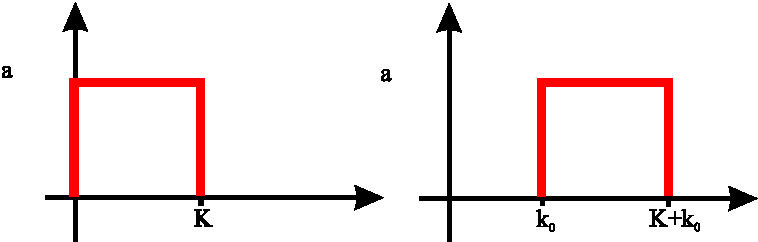
\includegraphics[width = 8cm]{ps/ZeitlicheVerschiebung}
\caption{\label{pic:VerschobenesRechteck} Veranschaulichung einer zeitlichen Verschiebung (Verzögerung)
um $k_0$.}
\end{center}
\end{figure}

\subsection{Darstellung diskreter Signale als Delta-Impulsfolgen}
\tbd{Alle digitalen Signale lassen sich als Summe von gewichteten und verschobenen Delta-Impulsen darstellen $x(k) = \sum x_{\kappa} \delta(k-\kappa)$}

\compileif{bBook}
{
\section{Darstellung und Generierung von Signalen in Matlab}
Für diesen Abschnitt siehe Matlab-Script. Ist hier nur aufgeführt als ein ToDo Punkt.

\subsection{Rauschsignale}
\subsection{determinierte Signale}
\subsubsection{Impulssignale}
\subsubsection{Periodische Signale}

\subsection{Darstellung}
\tbd{Plot, Stem. Hist}
}

\section{Übungen}
\subsection{Wiederholung des Stoffes und einfache Rechenaufgaben}
\begin{enumerate}
    \item Klassifizieren Sie folgende Signale anhand der im Skript angegeben Merkmale:
    \begin{enumerate}
        \item $si(t)$
        \item Das digitale (SP-DIF) und analoge Signal eines CD-Players
        \item Ein DVD Film
        \item Vielleicht ihr Beispiel
    \end{enumerate}
    \item Was ist die Grundvoraussetzung für eine erfolgreiche Digitalisierung?
    \item Warum verliert man Informationen bei der Digitalisierung?
    \item Warum lassen sich Funktionen mit Knickstellen (Bsp: Dreieck) nicht wirklich digitalisieren?
    \item Welches ist die höchste Harmonische einer aliasingfreien Dreieckschwingung mit der Grundfrequenz
    $f = 440$ Hz, bei einer Abtastrate von $f_s = 48000$ Hz?
    \item Zeigen Sie, dass $si(0) = 1$ ist!
    \item Zeichnen Sie $x(k) = 2\delta(k+2) - 0.5\delta(k-1) + 3\delta(k-2)$!
\end{enumerate}

\subsection{Aufgaben (Auf Klausurniveau)}
\begin{enumerate}
    \item Wie hoch ist die Leistung eines mittelwertfreien Dreieckssignals mit der Amplitude A?
    \item
    \item
\end{enumerate}

\compileif{bBook}{
\subsection{Matlab-Aufgaben}
\begin{enumerate}
    \item Programmieren Sie eine Funktion, die einen Mid-Tread Quantisierer mit einer Auflösung von
    4 Bit realisiert. Versuchen Sie so allgemein zu programmieren, dass Sie jederzeit die Auflösung
    ändern können.
    \item Programmieren Sie einen Rechtecksignal-Generator in Matlab, mit und ohne Aliasing.
    \item Erzeugen Sie eine Funktion die eine Delta-Impulsfolge mit vordefinierter Länge (Angabe
    in Sekunden und $f_s$) zurück gibt.
\end{enumerate}
}

\subsection{Transfer-Leistung}
\tbd{Fraglich ob hier möglich}
%
\compileif{bZusammenfassung}
{
\section{Zusammenfassung}
Die wichtigen Erkenntnisse aus diesem Kapitel sind:
\begin{itemize}
    \item Die Umwandlung analoger in digitale Signale erfolgt in zwei Schritten:
    \begin{itemize}
        \item Abtastung: verlustlos möglich, wenn gilt $f_{max} < f_s/2$ (Abtasttheorem)
        \item Quantisierung: verlustbehaftet
    \end{itemize}
    \item Mathematische Betrachtungen erfolgen meist mit diskreten Signalen (Annahme unendliche Genauigkeit)
    \item Signale lassen sich klassifizieren:
    \begin{itemize}
        \item Kanalanzahl
        \item Dimensionalität
        \item usw.
    \end{itemize}
    \item Es gibt Energie- und Leistungssignale:
    \begin{itemize}
        \item Energiesignale haben keine Leistung
        \item Leistungssignale haben eine unendliche Energie
     \end{itemize}
     \item Signale, die nicht stetig und/oder differenzierbar (\zB Rechteck, Dreieck)
     sind sind nicht bandbegrenzt und können
     deshalb nicht verlustlos diskretisiert werden.
    \item Dirac und Delta-Funktion stellen wichtige Elementarsignale dar.
\end{itemize}
}

\chapter{Systeme}
Betrachtet man die typische Nachrichtenübertragungskette, so ist
das Bindeglied zwischen Quelle und Senke der Kanal. Eine andere
allgmeinere Bezeichnung für den Kanal ist der Begriff System. Ganz
allgemein kann davon gesprochen werden, dass ein System
verschiedene (unterschiedliche) Signale miteinander verknüpft und
Beziehungen herstellt. Abbildung \ref{pic:SystembildAllgemein}
zeigt eine allgemeine Verknüpfung von Signalen.

\begin{figure}[h]
\begin{center}
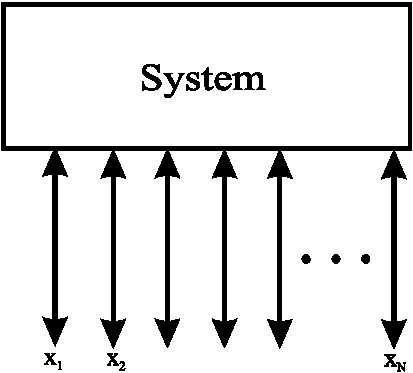
\includegraphics{psSys/SystemAllgemein}
\caption{\label{pic:SystembildAllgemein} Veranschaulichung eines
allgemeinen Systems, dass Signale miteinander verknüpft.}
\end{center}
\end{figure}

In den meisten Fällen, kann diese sehr allgemeine Verknüpfung
spezifiziert werden. Insbesondere haben wir häufig Eingangssignale
auf die das System reagiert und die daraus resultierenden
Ausgangssignale (siehe Abbildung \ref{pic:SystembildEinAus}).

\begin{figure}[H]
\begin{center}
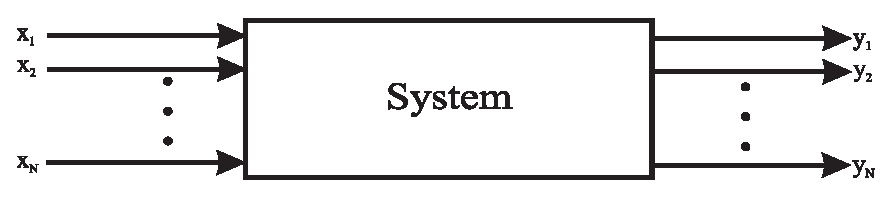
\includegraphics{psSys/SystemEinAus}
\caption{\label{pic:SystembildEinAus} Veranschaulichung eines
allgemeinen Systems, mit Signalen die als Ein- und Ausgangssignale
festliegen.}
\end{center}
\end{figure}

Durch diese sehr allgemeine Formulierung des Systembegriffs wird
auch deutlich, warum die Systemtheorie eine zentraler Punkt vieler
wissenschaftlicher Richtungen ist. Dies wird  auch deutlich, wenn
man einige Beispiele betrachtet:
\begin{itemize}
    \item HiFi-Verstärker: Ein System mit mehreren Eingängen und
    wenigen (meist zwei) Ausgängen
    \item Der Mensch: Ein sehr komplexes System mit vielen
    Eingängen (Sinnesorganen) und vielen Ausgängen (Muskeln)
    \item Computer: Viele Eingänge und Ausgänge
    \item Ihr Beispiel
\end{itemize}


\section{Eigenschaften und Klassifikation von Systemen}
Bei der Klassifikation der Systeme, können wir zunächst die
meisten Punkte, die wir für Signale erarbeitet haben, ebenfalls
anwenden.
\subsection{Wert- und Definitionsbereich}
Da wären zunächst die Frage, ob es sich bei dem betrachteten
System um ein analoges (wertkontinuierlich und zeitkontinuierlich)
oder um ein digitales (zeit- und wertdiskret) System  handelt. In
den nächsten Abschnitten werden wir uns zunächst nur mit digitalen
Systemen beschäftigen.

Die Klassifikation erfolgt also nach:

\wichtig{analoges System vs. digitales System}

\subsection{Kanalanzahl}
Die Kanalanzahl ist ebenfalls eine Möglichkeit ein System zu
beschreiben und zu klassifizieren, wobei als Besonderheit zu
beachten ist, dass Systeme auch die Kanalanzahl verändern können.
So kann \zB ein Monosignal (Gesang) auf zwei Kanäle aufgespalten
werden um so eine Positionierung in einem Stereosignal zu
ermöglichen.

\begin{figure}[H]
\begin{center}
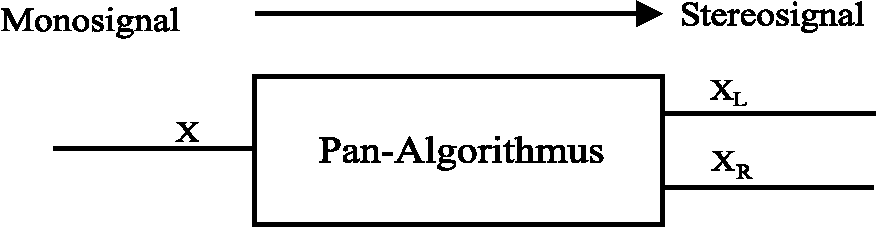
\includegraphics[width = 10cm]{psSys/PanAllgemein}
\caption{\label{pic:PanAlgo} Beispiel eines Systems mit einem
Eingang und zwei Ausgängen.}
\end{center}
\end{figure}

Wir können also Systeme nach der Kanalzahl der Ein- und Ausgänge
klassifizieren.

\wichtig{Einkanalig vs. Mehrkanalig}

Der allgemeinste Fall des mehrkanaligen Ein- und Ausgangs wird
als MIMO {\em Multiple Input Multiple Output} System bezeichnet.

\subsection{Dimensionalität}
So wie es ein- und mehrdimensionale Signale gibt, so können auch
Systeme in mehreren Dimensionen wirken. Ein einfaches Beispiel
wäre ein bildveränderndes System, dass natürlich zwei-dimensional
arbeiten müsste.

\wichtig{eindimensional vs. mehrdimensional}


\subsection{Rekursivität \label{ssec:Rekursion}}
Eine Eigenschaft, die wir bisher nicht mit Signalen erarbeitet
haben, ist die Frage, ob das System den eigenen Ausgang als
weiteren Eingang betrachtet. Abbildung \ref{pic:RekursivSystem}
zeigt ein System
dass sein Ausgangssignal auf den Eingang zurückführt. Ein solches
System bezeichnen wir als rekursives System.

\begin{figure}[H]
\begin{center}
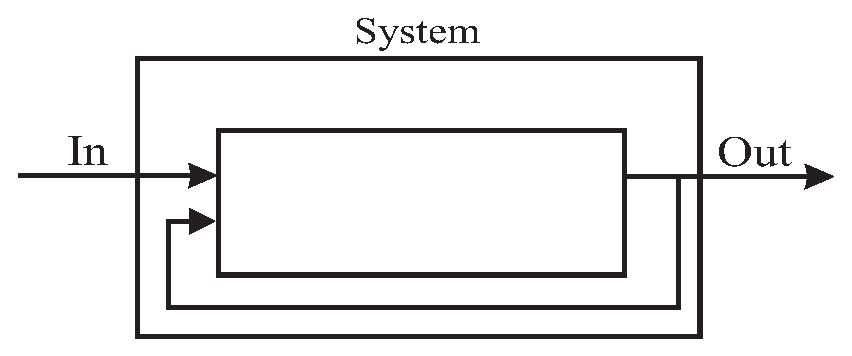
\includegraphics[width = 10cm]{psSys/RekursivSystem}
\caption{\label{pic:RekursivSystem} Allgemeines Blockdiagramm
eines einkanaligen rekursiven Systems.}
\end{center}
\end{figure}

Da es auch nicht-rekursive Systeme gibt, können wir folgende
Klassifikation einführen

\wichtig {rekursive vs. nicht-rekursive (transversal) Systeme }

Um die Wichtigkeit von rekursiven Systemen zu verdeutlichen,
nehmen wir einmal an, wir bräuchten ständig die Summe von mehreren
vergangenen Messwerten (oder ein Beispiel aus der Praxis ist der
30-Tage Durchschnitt bei der DAX-Analyse). Wir können diese Summe
immer wieder durch folgende Formel berechnen. Die Anzahl der
Messwerte, die wir verwenden ist durch $M$ symbolisiert.
\begin{equation}
y(k) = \sum_{m=0}^{M-1}x(k-m)
\end{equation}

Betrachtet man diese Rechenvorschrift, so fällt auf, dass
bestimmte Anteile immer wieder summiert werden und immer nur ein
neuer Wert hinzukommt und ein alter Wert herausfällt aus der
Summation. Dies ist in Abbildung \ref{pic:ErklaerungRekursion}
genauer gezeigt.

\begin{figure}[H]
\begin{center}
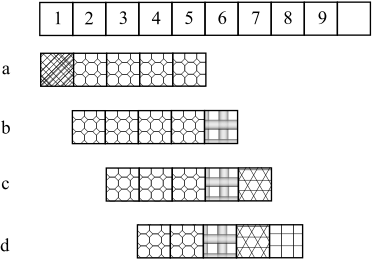
\includegraphics[width = 8cm]{psSys/DatenwerteRekursion}
\caption{\label{pic:ErklaerungRekursion} Erläuterung zur Anwendung
der Rekursion. Bei einer Summenbildung über die jeweiligen Zeilen
(a-d) sind die Summen zwischen a und b die achteckig gefüllten
Elemente bereits für a addiert worden. Man kann deshalb bei b
durch Subtraktion des gestrichelten ersten Elements und Addition
des Elements mit Kreuz direkt die neue Summe berechnen.}
\end{center}
\end{figure}

Man könnte also das Ausgangssignal des Systems auch durch folgende
Rechenvorschrift berechnen
\begin{equation} \label{eq:RekursionsBsp}
    y(k) = y(k-1) + x(k) - x(k-(M)).
\end{equation}

Es ist also möglich die Rechenleistung durch rekursive
Berechnungen zu verringern.

\subsection{Gedächtnis}
Bei der Rekursion haben wir gesehen, dass durch Speicherung der
Eingangsfolge und Speicherung des letzten Ausgangswertes sehr
einfach bestimmte Systeme realisiert werden können. Systeme die
Speicherelemente beinhalten werden gedächtnisbehaftet genannt.
Systeme bei denen der Ausgang nur von den Eingangssignalen, aber
nicht von dem vorherigen Zustand abhängig ist, sind gedächtnislos.
Ein Beispiel für ein gedächtnisloses System ist die Funktion $y(k)
= x^2(k)$.

\wichtig{Gedächtnisbehaftet vs. Gedächtnislos}

Die Gedächtnislänge eines Systems ist
durch die Möglichkeit der größten Signalverzögerung $k_0$
vorgegeben. Diese kann im transversalen oder im rekursiven Zweig
des Systems vorkommen. Der Hauptunterschied liegt im Einfluss des Gedächtnisses.
Bei ausschließlich transversalen Systemen bestimmt die Gedächtnislänge die
Einflusslänge. Für rekursive Systeme ist die Einflusslänge bis auf sehr wenige Ausnahmen unabhängig
von der Gedächtnislänge unendlich.

\subsection{Kausalität}
Die Kausalität ist für Systeme eine sehr wichtige Eigenschaft. Nur
bei kausalen Systemen ist die Ursache (Eingangssignal) zeitlich
immer vor der Wirkung (Ausgangssignal). Anders ausgedrückt das
Ausgangssignal darf nur von dem jetztigen Eingang und vorherigen
Eingangswerten abhängen, damit ein kausales System vorliegt.
Mathematisch kann dies durch
\begin{equation}
    y(k_0) = f\{x(k\leq k_0)\}
\end{equation}
ausgedrückt werden.

\subsection{Stabilität}
Eine andere sehr wichtige Eigenschaft für Systeme ist ihre
Stabilität. Stabile Systeme zeichnen sich dadurch aus, dass sie
auf ein begrenztes Eingangssignal mit einem begrenzten
Ausgangssignal reagieren (BIBO-Stabilität (Bounded input bounded
output)) Mathematisch muss folgendes als notwendige Bedingung gelten:
\begin{equation}
\mbox{wenn} \quad |x(k)| < \infty \quad \Rightarrow \quad |f\{x(k)\}| <
\infty
\end{equation}
\begin{example}
Sind die folgenden Systeme stabil?
\begin{itemize}
    \item $y(k) = x^2(k)$:\\
    Das System ist stabil, da alle möglichen Eingangswerte für
    x(k), die kleiner als $|\infty|$ sind, wieder auf Werte führen
    die kleiner als $\infty$ sind
    \item $y(k) = \log(x(k))$:\\
    Für $x(k) = 0$ ist $y(k) = -\infty$. Somit ist das System
    instabil.
\end{itemize}
\end{example}

\section{LTI-Systeme}
Eine besondere Klasse an Systemen stellen die linearen,
zeitinvarianten (LTI: linear and time-invariant) Systeme dar. Die
beiden Begriffe Linearität und Zeit-invarianz werden im weiteren
als Systemeigenschaften genauer beschrieben

\subsection{Linearität}
Lineare Systeme zeichnen sich dadurch aus, dass das sog.
Superpositionsprinzip (Überlagerungsprinzip) gilt. Dies bedeutet,
dass die additive Überlagerung der gewichteten Eingangssignale und
die Verknüpfung mit dem System genau zu dem gleichen Ergebnis
führt, wie die gewichtete additive Überlagerung der einzelnen
Signale am Ausgang des linearen Systems. Mathematisch ausgedrückt:
\begin{equation} \label{eq:Linearitaet}
    f\{a_1 x_1(k) + a_2 x_2(k) + \cdots + a_N x_N(k)\} = a_1 f\{x_1(k)\} + a_2 f\{x_2(k)\} + \cdots + a_N f\{x_N(k)\}
\end{equation}
wobei $f\{\cdot\}$ die Systemfunktion darstellt, $a_i$ die
linearen Gewichte und $x_i(k)$ die Eingangssignale. Abbildung
\ref{eq:Linearitaet} verdeutlicht den mathematischen Zusammenhang noch einmal
grafisch. Bei LTI-Systemen kann das System $H$ vor den Summationspunkt und vor
den linearen Gewichten $a_1$ und $a_2$ verschoben werden.

\begin{figure}[H]
\begin{center}
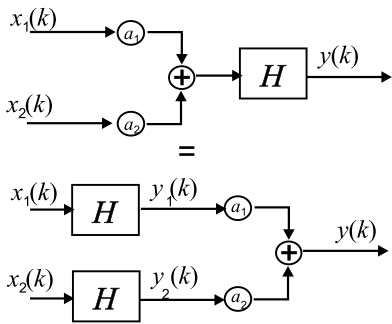
\includegraphics[width = 10cm]{psSys/LinearitaetErklaerung}
\caption{\label{pic:Linearitaet} Linearität bildlich erklärt}
\end{center}
\end{figure}

\begin{example}
Als Beispiel betrachten wir das System
\begin{equation}
y(k) = 2x(k) + 3x(k-1)
\end{equation}

Der Ausgang der einzelnen Eingangssignale $x_1(k)$ und $x_2(k)$
gewichtet ergeben.
\begin{eqnarray}
y_1(k) &= & (2x_1(k) + 3x_1(k-1))\\
y_2(k) &= & (2x_2(k) + 3x_2(k-1))\\
\end{eqnarray}
Der Ausgang ergibt sich zu
\begin{equation}\label{eq:Ausgangdirekt}
y(k) = a_1 y_1(k)+ a_2 y_2(k).
\end{equation}
und somit
\begin{equation}\label{eq:AusgangdirektFinal}
y(k) = 2 a_1  x_1(k) + 3 a_1 x_1(k-1)+  2 a_2 x_2(k) + 3 a_2 x_2(k-1) .
\end{equation}

Ein gemischtes und gewichtetes Eingangssignal ist gegeben durch
\begin{equation}
x_{mix} = a_1 x_1(k) + a_2 x_2(k)
\end{equation}
und das Ausgangssignal des System durch
\begin{eqnarray}
y(k) &=& 2x_{mix}(k) + 3x_{mix}(k-1)\\\nonumber
& = & 2(a_1 x_1(k) + a_2 x_2(k)) + 3(a_1 x_1(k-1) + a_2 x_2(k-1))\\\nonumber
& = & 2a_1x_1(k) + 2 a_2 x_2(k) + 3 a_1 x_1(k-1) + 3 a_2 x_2(k-1)
\end{eqnarray}
Dies ist im Vergleich zur Gleichung \ref{eq:Ausgangdirekt}
identisch. Somit ist das System linear.

Als zweites System testen wir $y(k) = x^2(k)$. Es ergeben sich
folgende Ausgangssignale:
\begin{eqnarray}
y_1(k) & = & x_1^2 (k)\\
y_2(k) & = & x_2^2 (k)\\
\Rightarrow y(k) &= &a_1 y_1(k) + a_2 y_2(k)\\
& = & a_1  x_1^2 (k) + a_2  x_2^2 (k)
\end{eqnarray}
bzw.
\begin{eqnarray}
y(k) &= &  x_{mix}^2 (k)\\
& = & \left( a_1  x_1 (k) + a_2  x_2 (k) \right)^2\\
 & = & a_1^2 x_1^2 (k) + 2a_1 a_2 x_1(k) x_2(k) + a_2^2 x_2^2 (k)
\end{eqnarray}
Die beiden Ausgangssignale sind nicht identisch. Dieses System ist
also nicht-linear.
\end{example}

\subsection{Zeit-Invarianz}
Von Zeitinvarianz spricht man, wenn das System seine Eigenschaften
nicht zeitlich ändert. Eine bestimmmte Verzögerung $k_0$ des
Eingangssignal führt also im Ausgang zu einem um die selbe Zeit
$k_0$ verzögerten Ausgangssignal. Mathematisch ausgedrückt:
\begin{equation}
y(k) = f\{x(k) \} \quad \Rightarrow y(k-k_0) = f\{x(k-k_0) \}
\end{equation}
mit $k_0$ als Angabe der diskreten Verzögerungszeit.

\begin{example}
Gegeben sind die beiden Systeme $y(k) = 2x(k)$ und $y(k) = x(2k)$.
Sind die Systeme zeitinvariant oder nicht?

Der Test erfolgt zum einen über die zeitliche Verschiebung des
Eingangssignal $x(k)$. Es ergibt sich ein neues Eingangssignal
$x(k-k_0)$. Für dieses neue Eingangssignal ist der Ausgang $y(k) =
2x(k-k_0)$. Zum anderen muss das Ausgangssignal des
Originaleingangssignals verschoben werden. Es ergibt sich zunächst
für den Ausgang $y(k) = 2 x(k)$. Dieses Signal wird jetzt um $k_0$
verschoben (Variablensubstitution $k' = k-k_0$). Der Ausgang ist
also $y(k') = y(k-k_0) = 2 x(k-k_0)$. Das System ist
zeit-invariant.

Beim zweiten System ergibt sich am Ausgang durch die Verschiebung
des Eingangssignals $y(k) = x(2k-k_0)$. Betrachtet man aber den um
$k_0$ verschobenen Ausgang ergibt sich durch die
Variablensubstitution $y(k-k_0) = x(2k-2k_0)$. Dieses System ist
also zeitvariant.
\end{example}


\subsection{Beschreibung durch Differenzengleichungen}
LTI-Systeme lassen sich stets durch Differenzengleichungen mit
festen Koeffizienten ausdrücken. Dies ist für nicht-rekursive
Systeme mit den Beispielen des Abschnittes über Linearität auch
leicht nachvollziehbar. Gleichzeitig gilt die selbe
Linearitätsbeziehung auch für den Ausgang des Systems. Betrachtet
man nun ein System, dass rekursiv ist, so kommen als neue Terme
nur vergangene Systemantworten mit linearen Faktoren gewichtet
(multipliziert) hinzu. Damit sind auch alle durch folgende
Gleichung aufgebauten rekursiven Systeme linear.
\begin{equation}
\sum_{i = 0}^{N} a_i y(k-i) = \sum_{j = 0}^{M}b_j x(k-j)
\end{equation}
Um nun nur den Ausgang des Systems zu betrachten, wird vereinbart,
dass $a_0 = 1$ ist\footnote{Dies könnte jederzeit durch eine
Division durch $a_0$ erreicht werden.}. Für den Ausgang eines
kausalen Systems gilt dann
\begin{equation}
y(k) = -\sum_{i = 1}^{N}a_i y(k-i) + \sum_{j = 0}^{M}b_j
x(k-j)
\end{equation}

%Die Summe für die rekursiven Signalanteile beginnt bei 1, da der
%0. Koeffizient eigentlich dem aktuellem Ausgangssignal zugeordnet
%ist, so wie $b_0$ dem aktuellen Eingangswert zugeordnet ist. Da
%wir aber eine ungewichtete Ausgangsfolge haben wollen, wird $a_0$
%auf eins normiert. Ist dieser Wert bei einer gegebenen Aufgabe
%ungleich null, so müssen alle Koeffizienten $a_i$ und $b_j$ durch
%$a_0$ dividiert werden.

Um zu wissen, welche Folge $y(k)$ am Ausgang herauskommt, ist es
notwendig den aktuellen und die vergangenen Eingangssignale $x(k)$
zu kennen. Zusätzlich muss aber auch bekannt sein, wie die inneren
Zustände des Systems aussehen. Es müssen also die vorherigen
Ausgangswerte bekannt sein, um die vollständige Beschreibung zu
gewährleisten. Häufig wird vereinfacht angenommen, dass das System
in Ruhe war und deshalb gilt
\[
   y(k-i) = 0 \qquad \forall \qquad i>0.
\]

\subsubsection{Einführung der Systemantwort auf die Delta-Impulsfolge}
Die Systemantwort auf die Delta-Impulsfolge $\delta(k)$ wird als
Impulsantwort $h(k)$ bezeichnet und charakterisiert ein LTI-System
vollständig. Für nicht-rekursive Systeme mit einer endlichen
Anzahl von Koeffizienten, also $M< \infty$ ist die Impulsantwort
endlich. Deshalb werden diese Systeme auch als {\em Finite Impulse
Response} (FIR)-Systeme bezeichnet. Bei rekursiven Systeme gilt
dies im allgemeinen nicht. Diese Systeme werden im
englischsprachigen Raum, deshalb als {\em Infinite Impulse
Response} (IIR)-Systeme bezeichnet.

\begin{example}

Nehmen wir an, wir suchen die Impulsantwort des LTI-Systems $y(k)
= r_0 x(k) + r_1 x(k-1) - r_2 x(k-2)$. Errechnet man nun den
Ausgang für alle $k$ und setzt jeweils für x(k) die Impulsfolge
ein, so ergibt sich die Impulsantwort\footnote{Die Impulsantwort wird hier
in einer Vektorschreibweise eingeführt.} $h(k) = [r_0 \,\, r_1 \,\,
-r_2]$ für $0 \leq k \leq 2$. Das betrachtete System
war ein FIR-System. Ganz allgemein ergibt sich für FIR-Systeme
immer, dass $h(k) = b_k$ ist.

Für IIR-Systeme ist die Berechnung der Impulsantwort nicht so
trivial. Betrachten wir das System
\[
y(k) = \alpha y(k-1) + \beta x(k).
\]
Als Eingangssignal nutzen wir erneut $x(k)= \delta(k)$.
Die Ausgangsfolge für
alle $k$ berechnet, ergibt
\[h(k) = [\beta \,\, \alpha \beta \,\,
\alpha \alpha \beta \,\, \cdots \,\, \alpha^{k}\beta].
\]
Die Impulsantwort endet nicht.
\end{example}

Für viele Probleme reicht es aber aus, die Impulsantwort nur so
weit zu betrachten, wie sich noch signifikante Werte ergeben.
Signifikant kann dabei zum Beispiel sein zu testen, ob die Werte
von $h(k)$ kleiner als der millionste Teil des maximalen Wertes
von $h(k)$ ist.

\wichtig{Die Impulsantwort eines Systems ist der Ausgang des
Systems, wenn die Eingangsfolge die Delta-Impulsfolge ist. Die
Impulsantwort beschreibt ein LTI-System vollständig}

\wichtig{Nicht-rekursive Systeme haben eine endliche Impulsantwort.
Sie werden als FIR-Systeme bezeichnet.}

\subsection{Faltung als Verknüpfung von LTI-Systemen und Signalen}
Bisher haben wir nur gesehen, wie die Eingangssignale durch die
Differenzengleichung zum Ausgangssignal werden. Es gibt aber eine
allgemeinere Vorschrift, die direkt mit der Impulsantwort zusammen
hängt.

Zur Veranschaulichung wird zunächst ein einfaches Beispiel berechnet.
Das Eingangssignal ist
durch zwei Werte gegeben, wir nehmen an $x(0)= 0.5$ und $x(1) =
1.5$. Das System ist durch $y(k) = -0.25x(k) + 0.5x(k-1)$
definiert. Wie lautet die Ausgangssfolge? Man könnte jetzt einfach
die verschiedenen Zeitpunkte $k$ annehmen und das Ergebnis direkt
hinschreiben. In Tabellenform wäre das Ergebnis:

\begin{center}
\begin{tabular}{|c|c|c|c|}\hline
$k$ & $x(k)$ & $x(k-1)$ & $y(k)$ \\\hline
0 & 0.5 & 0   & -0.125\\ \hline
1 & 1.5 & 0.5 & -0.125\\ \hline
2 &  0  & 1.5 &  0.75\\ \hline
3 &  0  &  0  &    0\\ \hline
\end{tabular}
\end{center}

Für dieses einfache Beispiel ist das noch leicht möglich, bei längeren Folgen
wäre diese Lösung unpraktisch.
Statt dessen versuchen wir einen allgemeineren
Lösungsweg zu finden. Die Eingangsfolge $x(k)$ lässt sich für alle $k$
mit Hilfe der delta-Folge $\delta(k)$ durch
\begin{equation}\label{eq:diracinput}
    x(k) = 0.5 \delta(k) +  1.5 \delta(k-1)
\end{equation}
vollständig beschreiben.

Mit dem Gesetz der Linearität und dem Wissen der Impulsantwort
$h(k) = [-0.25 \:\, 0.5]$, ergibt sich die Antwort für $y(k)$ aus
der Summe der gewichteten und verschobenen Impulsantworten, da
jede der delta-Folgen die Impulsantwort als Systemantwort hervor
ruft.

Allgemeiner lässt sich sagen, jedes diskrete Eingangssignal lässt
sich in viele kleine Einzelimpulse zerlegen. Wir haben es also
immer mit einer gewichteten Summe von Delta-Impulsfolgen zu tun.
Aus dem letzten Abschnitt haben wir kennengelernt, dass die
Impulsantwort ein LTI-System vollständig beschreibt. Außerdem gilt
für LTI-Systeme das Superpositionsprinzip. Das Ausgangssignal
eines LTI-Systems kann deshalb durch eine mit linearen
Koeffizienten gewichtete Addition der zeitlich verschobenen
Impulsantwort berechnet werden.

Um dies zu veranschaulichen, ist in Abbildung
\ref{pic:Faltungserklaerung} diese Zerlegung für ein Beispiel
durchgeführt. Bild a) zeigt die Eingangssfolge $x(k) = [1\,\, 0.5
\,\, 1]$ , Bild b) das System $h = [0.5 \,\,\,  0.75 \; 1]$.
Zerlegt man nun die Eingangsfolge in drei Einzelimpulse ergeben
sich die drei Bilder c,e,g. Jeder dieser Einzelimpulse erzeugt
eine verschobene und gewichtete Version der Impulsantwort (Bild
d,f,h). Das Ausgangssignal (i) ergibt sich schlussendlich aus der
Summe dieser Ausgangssignale.
\begin{figure}[H]
\begin{center}
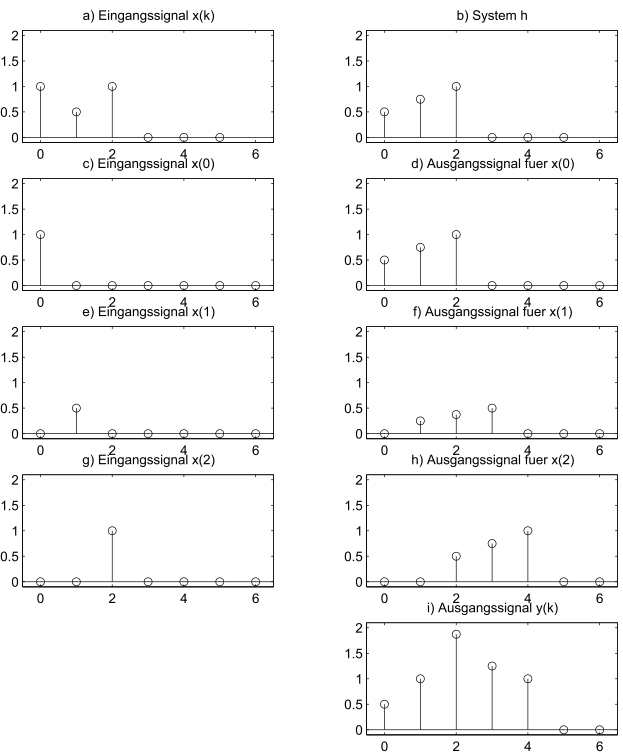
\includegraphics[width = 16cm]{psSys/FaltungErklaerung}
\caption{\label{pic:Faltungserklaerung} Einfache grafische
Erklärung der Faltung}
\end{center}
\end{figure}

Allgemein und mathematisch wird dies durch
\begin{equation}
    y(k) = \sum_{\kappa = -\infty}^{\infty} h(\kappa) x(k-\kappa)
\end{equation}
ausgedrückt. Diese Summe wird als Symbol durch $\ast$ dargestellt und als
Faltungsumme bezeichnet:
\begin{eqnarray}
    y(k) &=& \sum_{\kappa = -\infty}^{\infty} h(\kappa) x(k-\kappa)\\
        & = & h(k) \ast x(k)
\end{eqnarray}

\subsubsection{Eigenschaften der Faltung}
Der Faltungsoperator ($\ast$) kann wie die Multiplikation aufgefasst werden.
Es gelten die folgenden mathematische Gesetze:
\begin{itemize}
\item Kommutativgesetz
\begin{equation}\label{eq:FaltungKommu}
    x(k) \ast h(k) = h(k) \ast x(k)
\end{equation}
\item Assoziativgesetz
\begin{equation}\label{eq:FaltungAssoz}
   ( x(k) \ast y(k)) \ast h(k) =  x(k) \ast (y(k) \ast h(k))
\end{equation}
\item Distributivgesetz
\begin{equation}\label{eq:FaltungDistrib}
   ( x(k) + y(k)) \ast h(k) =  x(k)\ast h(k) +  y(k) \ast h(k)
\end{equation}


\end{itemize}

\subsubsection{grafische Faltung}
Die Berechnung des Faltungsproduktes lässt sich auch grafisch gut
veranschaulichen. Dazu betrachten wir Abbildung
\ref{pic:GraphischeFaltungErk}. Die beiden zu faltenden Folgen $x(k)$
und $h(k)$ sind in a) gezeigt. Das Faltungsergebnis erhält man,
wenn man eine der Folgen zeitlich spiegelt b), also an der y-Achse
umklappt und diese Folge über das andere Signal schiebt c). Der
Ausgang d) ergibt sich immer aus der Summe der sich überlappenden
und miteinander multiplizierten Einzelimpulse der beiden Folgen.

\begin{figure}[H]
\begin{center}
\includegraphics[width = 12cm]{psSys/FaltungsErklaerungCorel}
\caption{\label{pic:GraphischeFaltungErk} Erklärung der grafischen
Faltung}
\end{center}
\end{figure}

Die Länge der Ausgangsfolge ergibt sich aus der Addition der
Länge der Eingangsfolge $M$ und der Länge der Impulsantwort $K$ zu
\begin{equation}
    N = M + K - 1.
\end{equation}
Dies ist auch anhand der beiden grafischen Beispiele
leicht zu sehen.

\tbd{grafische Faltung bei analogen Signalen}

\compileif{bBook}
{
\section{Systeme und Matlab}
Auch hier gilt, siehe Script.
\subsection{Test auf Nicht-Linearität und Zeitvarianz}
\subsection{Faltung}
}

\section{Übungen}
\subsection{Wiederholung des Stoffes und einfache Rechenaufgaben}
\begin{enumerate}
    \item Ist ein Quantisierer ein lineares System, da ja von
    linearer Quantisierung gesprochen wird? Begründen Sie ihr
    Antwort.
    \item Sind die folgenden Systeme zeitinvariant, kausal und linear? Begründen Sie ihre Antwort.
    \begin{itemize}
        \item{$y(k) = x(k) + 2d $ mit $d\neq 0$}
        \item $y(k) = a_1 x(k-2) + a_2 x(k-3)$
        \item $y(k) = k x(k-1) + x(k-2)$
        \item $y(k) = log_{10}( x(k-2)) + 3 x(k-1) $
    \end{itemize}
    \item Falten Sie die folgenden vier Signale jeweils grafisch mit sich selbst und mit allen anderen
    Signalen.
    \begin{figure}[H]
    \begin{center}
    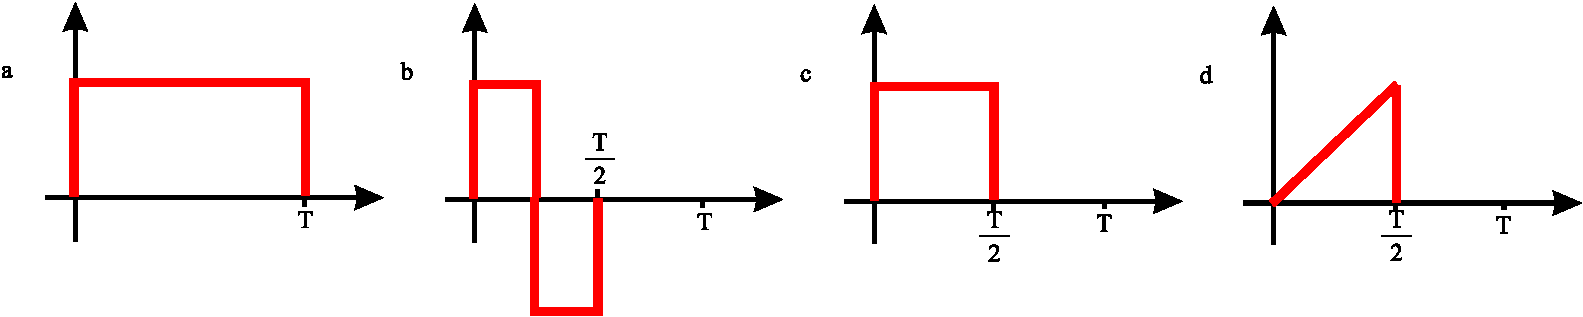
\includegraphics[width = 15cm]{psUeb/GraphikFaltung}
    \caption{\label{pic:UebungGraphischeFaltung}Testsignale zum Üben der grafischen Faltung}
    \end{center}
    \end{figure}
    \item Zeigen Sie, dass das Kommutativgesetz der Faltung allgemein gilt.
\end{enumerate}
\subsection{Aufgaben (Einige auf Klausurniveau)\label{ssec:Aufgaben}}
\begin{enumerate}
    \item \label{Aufg:impulsfolge}Geben sie die Impulsantwort für die folgenden
    Differenzengleichungen an. Brechen
    Sie bei unendlichen Folgen nach $k=10$ ab. Nehmen sie an, dass sich das System zum Zeitpunkt $k=0$
    in Ruhe befand.
    \begin{enumerate}
        \item $y(k) = 0.5x(k-1)+ 0.3x(k-2)+ 0.4x(k-3) - 0.4 x(k-4)$
        \item $y(k) = y(k-1)+0.5x(k)$
        \item $y(k) = 0.25 x(k-1)+0.75 y(k-1) - 0.75y(k-3)$
    \end{enumerate}
    \item Gegeben ist das System $0 = \frac{1}{k} x(k) + 2x(k-2) - 0.5y(k-1)$. Begründen Sie
    Linearität und Zeit-Invarianz bitte mathematisch formal!

    \item
\end{enumerate}

\compileif{bBook}
{
\subsection{Matlab-Aufgaben}
\begin{enumerate}
    \item Testen Sie folgende Systeme auf Zeitinvarianz und Linearität durch Rauschfolgen als
    Eingangssignale. Haben Sie im Hinterkopf, dass Sie mit Zahlentests nichts beweisen können.
    Eine Aussage ist nur für Nicht-Linearität und Zeitvarianz möglich. Dies ergibt sich, wenn
    der Test fehl schlägt, da {\em ein} Gegenbeispiel ausreicht um Linearität oder Zeitinvarianz
    auszuschließen.
    \begin{itemize}
        \item $y(k) = x(k) + y(k-1)$
        \item $y(k) = 3 y(k-1) + 2 x(k-1) + x(k)$
        \item $y(k) = k x(k-1) + x(k-2)$
        \item $y(k) = log_{10} x(k-2) + 3 y(k-1) $
    \end{itemize}
    \item Erzeugen Sie eine Funktion die eine Delta-Impulsfolge mit vordefinierter Länge zurück gibt.
    \item Nutzen Sie diese Funktion, um ihre Ergebnisse aus Abschnitt \ref{ssec:Aufgaben} Aufgabe \ref{Aufg:impulsfolge} zu überprüfen.
    \item Erzeugen Sie kurze Sequenzen mit $T = 12$ Werten um die oben gezeigten Signale zu approximieren.
    Überprüfen Sie Ihre Ergebnisse mit dem {\tt conv}-Befehl.
\end{enumerate}
}
\subsection{Transfer-Leistung}
\begin{enumerate}
    \item
    \item
    \item
\end{enumerate}
%
\compileif{bZusammenfassung}
{
\section{Zusammenfassung}
Die wichtigen Erkenntnisse aus diesem Kapitel sind:
\begin{itemize}
    \item Lineare zeitinvariante (LTI)-Systeme stellen eine wichitge Klasse der Systeme dar.
    \item LTI-Systeme lassen sich vollständig durch Differenzengleichungen beschreiben.
    \item Die Faltung verknüpft LTI-Systeme und Signale
    \item Die Impulsantwort ist das Ausgangssignal eines Systems, wenn die Delta-Folge als
    Eingang gewählt wurde. Sie beschreibt ein LTI-System ebenfalls vollständig.
\end{itemize}
}
%\newpage

%\section{Lösungen zu den Übungsaufgaben}

\chapter{z-Transformation}
In diesem Abschnitt werden wir die z-Transformation als ein
wichtiges Werkzeug zur Analyse und zum Verständnis
von LTI-Systemen und ihrer Eigenschaften einführen.
Es werden durch die z-Übertragungsfunktion und dem Pol-Nullstellenplot neue
Beschreibungsformen für LTI-Systeme aufgezeigt.
Insbesondere wird eine Möglichkeit angegeben, um die Stabilität rekursiver LTI-Systeme
zu testen.

\tbd{Beispiel bringen mit Programm (Minihost, Asio4All, pcx) zur Motivation}

\section{Einführung}
Um die Nützlichlkeit dieses Werkzeuges zu untermalen, wollen wir
zunächst von einfachen Beispielen ausgehen.

Angenommen auf ein Sparbuch wird ein bestimmter Geldbetrag $S$
eingezahlt und dieser Betrag wird jährlich mit einem Zins $p$
verzinst. Eine mathematische Darstellung dieses Sachverhalts ergibt sich durch Nutzung des Delta-Impulses gewichtet
mit dem Geldbetrag und einer einfachen Rekursion, wobei ein leeres Konto als Startwert vorliegt. Es gilt also $y(k-1) = 0$.
\begin{equation}\label{eq:ZinsRekursion}
y(k) = (1+p) y(k-1) + S \delta(k)
\end{equation}

Dies ist eine andere Darstellung der Zinseszinsrechenregel. Diese lautet
\begin{equation}
    \mbox{Geld} = S (1+p)^{\mbox{Jahre}}
\end{equation}

Die Anzahl der Jahre ist in \ref{eq:ZinsRekursion} in der Anzahl
der Rekursionen versteckt. Die zweite Form ist eine direkte
Berechnung.
%Diese beiden Möglichkeiten hatten wir auch schon beim
%einführenden Beispiel zur Rekursion gesehen (vergleiche Abschnitt
%\ref{ssec:Rekursion}).

Nun lassen sich aber nicht für alle Rekursionssysteme solche
einfachen direkten Rechenvorschriften angeben. Aber wie ist der mathematische Zusammenhang zwischen den beiden möglichen Lösungen?

In der Rekursionsformel:
\begin{equation}\label{eq:ZinsRekursionWiederholung}
    y(k) = (1+p) y(k-1) + S \delta(k)
\end{equation}
ergibt sich durch Variablensubstitution $c = 1+p$.
\begin{equation}\label{eq:ZinsRekursionMitc}
    y(k) = c y(k-1) + S \delta(k)
\end{equation}
Diese Form wird jetzt auf beiden Seiten mit der Summe $\sum_{k =
-\infty}^{\infty}z^{-k}$ multipliziert. Ein Schritt der
mathematisch erlaubt ist, da er auf beiden Seiten des
Gleichungssystems durchgeführt wird.
\begin{equation}
\sum_{k = -\infty}^{\infty} y(k) z^{-k} = \underbrace{c \sum_{k =
-\infty}^{\infty} y(k-1) z^{-k}}_{\mbox{1. Summand}} +
\underbrace{S \sum_{k = -\infty}^{\infty} \delta(k)
z^{-k}}_{\mbox{2. Summand}}
\end{equation}
Mit Hilfe der abkürzenden Schreibweise 
\begin{equation}\label{eq:Def:zTrafo}
Y(z) = \sum_{k = -\infty}^{\infty} y(k) z^{-k} .
\end{equation}
ergibt sich bei dem 2. Summanden nur ein Element der Summe den Wert
$S$, da die $\delta$-Folge nur bei $k = 0$ einen Wert ungleich
Null hat.

Zusätzlich kann der 1. Summand durch eine
Variablensubstitution $k' = k-1$ umgeformt werden.
\begin{equation}\label{eq:zTrafo:Example1Subst}
    c \sum_{k =
-\infty}^{\infty} y(k-1) z^{-k} = c \sum_{k' = -\infty}^{\infty}
y(k') z^{-k'-1} =c z^{-1}\sum_{k' = -\infty}^{\infty} y(k')
z^{-k'}=c z^{-1} Y(z)
\end{equation}

Somit ergibt sich
\begin{equation}\label{eq:zTrafo:Example1}
    Y(z) = c z^{-1} Y(z) + S .
\end{equation}
Umgestellt folgt
\begin{equation}\label{eq:ztrafo:Example1:zLoesung}
    Y(z) = \frac{S}{1-c z^{-1}} .
\end{equation}

Um zur Lösung für das Ausgangssignal zu kommen, wird die Summenformel für eine geometrische Reihe eingeführt.
\begin{equation}\label{eq:Def:geometrischeReihe}
    \sum_{k = 0}^{\infty} q^k = \frac{1}{1-q}  \quad \mbox{wenn} \quad
    |q|<1
\end{equation}

Für Gleichung \ref{eq:ztrafo:Example1:zLoesung} ergibt sich also
\begin{equation}\label{eq:zTrafo:Example1:kLoesung1}
    \frac{S}{1-c z^{-1}} = S \sum_{k = 0}^{\infty} (c z^{-1})^k = S \sum_{k = 0}^{\infty} c^k z^{-k}
\end{equation}

Vergleicht man diese Lösung mit \ref{eq:Def:zTrafo} so ergibt sich
\begin{equation}\label{eq:zTrafo:Example1:kLoesung2}
    y(k) = \bigg\{ \begin{array}{lcc}
      S c^k & & k \geq 0\\
        0  & & k<0
    \end{array} = S(1+p)^k \gamma(k)
\end{equation}
mit $\gamma(k)$ als Sprungfolge (siehe Gl.
\ref{eq:Def:Sprungfolge}).

Dies entspricht der vorher bekannten Lösung für die
Zinseszinsformel.


\section{Definition}
Für eine verkürzte
Schreibweise wird für die z-Transformation folgendes Symbol eingeführt
\begin{equation}\label{eq:Def:Ztrafo}
    \ZT{ \cdot }= \sum_{k = -\infty}^{\infty} (\cdot) z^{-k} \Mit z \in \mathbb{C}
\end{equation}

Es gilt also
\begin{equation}\label{eq:yExample}
    Y(z) =\ZT{y(k)}
\end{equation}
Die Rechenvorschrift führt dazu, dass die diskrete Eingangsfolge
$y(k)$ abgebildet wird auf eine komplexe Ebene. Man spricht
deshalb auch von Zeitbereichsdarstellung und
Bildbereichdarstellung. Um die Korrespondenz zu symbolisieren wird
häufig der sog. ''Transformationsknochen'' verwendet.
\begin{itemize}
    \item Hintransformation: $y(k)\HinTrans Y(z)$ oder bei Gleichungsabfolgen $\HinTransV$
    \item Rücktransformation: $Y(z) \RueckTrans y(k)$ oder $\RueckTransV$
\end{itemize}

Damit eine z-Transformation gültig ist, muss zusätzlich gelten,
dass die Summe in Gl. \ref{eq:Def:Ztrafo} kleiner unendlich ist.
Dies ist für alle endlichen Folgen gegeben, wenn
keiner der Folgenwerte unendlich ist. Bei unendlichen Folgen ist dies
nicht immer gewährleistet.und hängt auch
direkt von der Wahl des $z$ ab. Deshalb gehört zu einer
vollständigen Beschreibung der z-Transformation auch immer die
Bereichsangabe von $z$ in der die Summe konvergiert. Man spricht deshalb vom sogenannten
Konvergenzgebiet {\em Region of Convergence}.
Zur Beschreibung des Konvergenzgebietes reichen die
Angaben der Radien $r = |z|$ der komplexen Zahlen aus. Für das
Konvergenzgebiet ergibt sich entweder das Gebiet inner- oder außerhalb einer
Kreisfläche oder das Gebiet hat die Form eines Kreisringes in der z-Ebene.

\begin{figure}[H]
\begin{center}
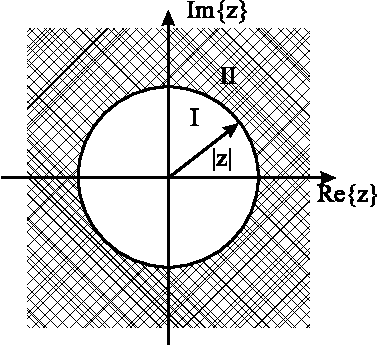
\includegraphics[width = 8cm]{psZ/ROC_Kausal}
\caption{\label{pic:ROC_Kausal} Veranschaulichung des Konvergenzgebietes
bei der z-Transformation. In diesem Beispiel für eine kausale Folge (ROC außerhalb).}
\end{center}
\end{figure}

\begin{example}
%\begin{minipage} {14cm}
\label{Bsp:z_TrafoUndROC} Betrachtet man die kausale Folge (siehe Abbildung \ref{pic:zFolgnPic}a)
(Sie entspricht dem Sparbuchbeispiel mit einem Startkapital von
0.5 und 50\% Kontokosten (Also einer ziemlich schlechten Geldanlage).)
\begin{eqnarray} \label{eq:BspKausaleFolge}
    x(k) &=& [0.5 \:\: 0.5^2 \:\: 0.5^3 \:\: \cdots \:\: 0.5^k]\\
         & = & 0.5^k \gamma(k) \qquad \fuer k \geq 0 ,
\end{eqnarray}
so ergibt sich die z-Transformierte als
\begin{equation}
    X(z) = \sum_{k = -\infty}^{\infty} 0.5^k \gamma(k)z^{-k}
    = \sum_{k = 0}^{\infty} 0.5^k z^{-k} =
    \sum_{k = 0}^{\infty} (0.5z^{-1})^{k}
\end{equation}
bzw. mit der Umformung durch die geometrische Reihe
\begin{equation}
    X(z) = \frac{1}{1-0.5z^{-1}} = \frac{z}{z-0.5},
\end{equation}
wobei das Konvergenzkriterium der geometrischen Reihe zusätzlich
\begin{equation}\nonumber
    |0.5z^{-1}| = \frac{0.5}{z} < 1 \qquad \Rightarrow \qquad |z| > 0.5
\end{equation}
fordert.

\begin{figure}[H]
\begin{center}
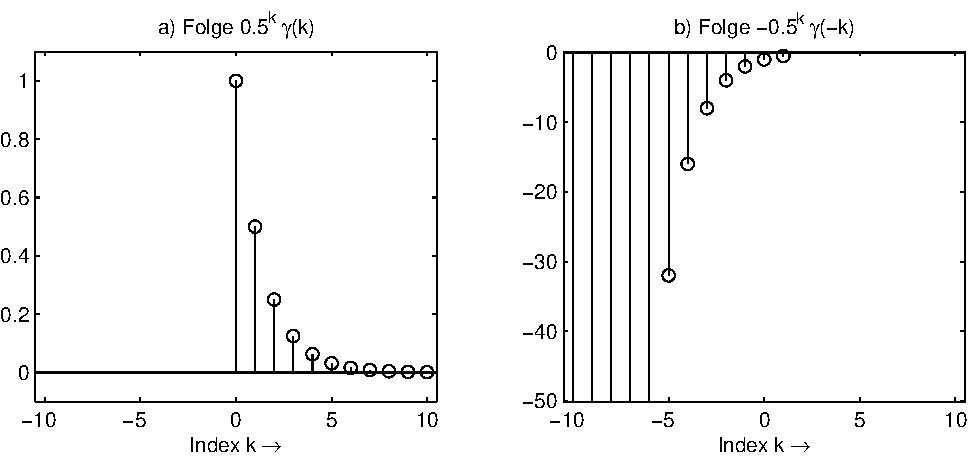
\includegraphics[width = 10cm]{psZ/zFolgenPic}
\caption{\label{pic:zFolgnPic} a) kausale Folge $0.5^k \gamma(k)$ für $ k \geq 0 $
und b) nicht-kausale Folge $-0.5^k \gamma(-k-1)$ für $k < 0$.}
\end{center}
\end{figure}

Im folgenden soll nun eine sehr ähnlichen Folge, nämlich
dem nicht-kausalen, negativen äquivalent zu \ref{eq:BspKausaleFolge}
\begin{equation}\nonumber
    x(k) = -0.5^k \gamma(-k-1) \qquad \fuer k < 0
\end{equation}
betrachtet werden (siehe Abbildung \ref{pic:zFolgnPic}b).
Berechnet man die z-Transformierte ergibt sich mit einer Variablensubstitution $k = -m$
\begin{eqnarray}\nonumber
    X(z) &=& - \sum_{k = -\infty}^{-1} 0.5^k z^{-k} \\
    & = &- \sum_{k = -\infty}^{-1} (0.5^{-1}z)^{-k} \\
    & = &- \sum_{m = 1}^{\infty} (0.5^{-1}z)^{m}
\end{eqnarray}
Nutzt man jetzt eine alternative Formulierung der unendlichen geometrischen
Reihe
\begin{equation}\nonumber
    \sum_{m = 1}^{\infty} x^m = \frac{x}{1-x}
\end{equation}
so ergibt sich
\begin{equation}\nonumber
    X(z) = - \frac{0.5^{-1}z}{1-0.5^{-1}z} = \frac{z}{z-0.5}
\end{equation}
Wir erhalten also die gleiche z-Transformation für unterschiedliche Folgen, wobei aber
die Konvergenz der geometrischen Reihe für die anti-kausale Folge ein Konverzgebiet
\begin{equation}\nonumber
    |z| < 0.5
\end{equation}
fordert. Abbildung \ref{pic:ROC_AntiKausal} zeigt das dazugehörige Konvergenzgebiet
in der z-Ebene.
Man erkennt somit, warum eine Angabe des ROC bei der z-Transformation notwendig ist, um eine
eindeutige Berechnung und Zuordnung zu gewährleisten.
\begin{figure}[H]
\begin{center}
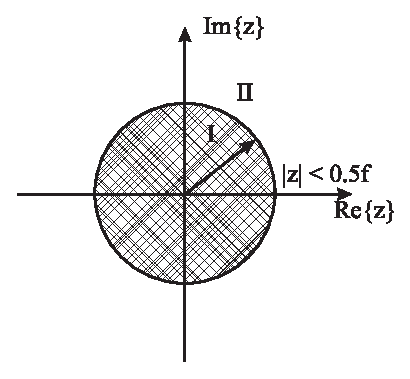
\includegraphics[width = 8cm]{psZ/ROC_AntiKausal}
\caption{\label{pic:ROC_AntiKausal} Veranschaulichung des Konvergenzgebietes
bei der z-Transformation. In diesem Beispiel für eine anti-kausale Folge (ROC innerhalb) mit
$|z| < 0.5$.}
\end{center}
\end{figure}
%\addtolength{\hoffset}{-3cm}
\hspace{0.1mm}
\end{example}
%\end{minipage}

\section{Rechenregeln}
Die z-Transformation erleichtert das
Rechnen von Differenzengleichungen. Wir werden deshalb im weiteren
einige häufig verwendete Rechenregeln und Korrespondenzen
einführen.

\subsection{Linearität}
Die z-Transformation ist eine lineare Transformation. Es gilt:
\begin{equation}\label{eq:zTrafo:Linearitaet}
  a_1 x_1(k) + a_2 x_2(k) \HinTrans a_1 X_1(z) + a_2 X_2(z)
\end{equation}

\subsection{Verschiebung}
Die zeitliche Verschiebung der diskreten Folge haben wir bereits
in den Beispielen ausgiebig verwendet. Es gilt:
\begin{equation}\label{eq:zTrafo:Verschiebungssatz}
    \mathcal{Z}\{y(k-k_0)\} = z^{-k_0} Y(z)
\end{equation}

\section{Rück-Transformation}
Wir haben gesehen, dass die z-Transformation eine diskrete Folge
in eine kontinuierliche komplexe Ebene transformiert. In den
Beispielen hatten wir es für die Rücktransformation in den
Zeitbereich stets mit einfachen gebrochen rationalen Funktionen zu
tun, die direkt auf eine bestimmte Folge führten. Dies ist nicht
immer möglich. Die allgemeinste Version der z-Rücktransformation
ist durch das Umlaufintegral
\begin{equation}\label{eq:zRuek:Def}
    x(k) = \oint_C X(z) z^{k-1} dz
\end{equation}
gegeben. Dies bedeutet wir umlaufen die komplexe Ebene auf dem
Kreis C im mathematisch positiven Sinn (Gegenuhrzeigersinn) und
integrieren die eingeschlossene Fläche. Dies ist nicht immer
möglich. Ob die Möglichkeit besteht hängt direkt davon ab, wie das
Konvergenzgebiet definiert ist. Auf die  explizite Behandlung der
Thematik wird hier nicht eingegangen, statt dessen wird auf \cite{OS99}
verwiesen, die Stichworte, die man sich im
Zusammenhang mit der Rücktransformation merken sollte sind:
Cauchy-Integral, Laurent-Reihe, Residuensatz.

In vielen Fällen kann auf die Lösung des Integrals verzichtet
werden. Statt dessen sind häufig Lösungen über
Partialbruchzerlegung (siehe Beispiele) und/oder
Korrespondenztabellen möglich


\subsection{Korrespondenztabelle}

Viele Systeme und Signale lassen sich auf einfache Grundformen
zurückführen. Für diese Grundformen kann für die Hin- und
Rücktransformation folgende Tabelle verwendet werden.

\begin{tabular}{|c|c|c|}
  \hline
  % after \\: \hline or \cline{col1-col2} \cline{col3-col4} ...
  Zeitbereich $y(k)$ & Bildbereich $Y(z) = \ZT{y(k)}$ & Konvergenzgebiet \\
  \hline
  $\delta(k)$     & 1                                 & $\forall z$\\
  $\gamma{k}$     & $\frac{z}{z-1} = \frac{1}{1-z^{-1}} $ & $|z|>1$ \\
  $k \gamma(k)$   & $\frac{z}{(z-1)^2}$               & $|z|>1$\\
  $e^{-\alpha k}\gamma (k)$ & $\frac{z}{z-e^{-\alpha}}$  & $|z|>e^{-\alpha}$\\
  $\alpha^k \gamma (k)$ & $\frac{z}{z-\alpha}$ & $|z| > \alpha$ \\
  $\cos(\omega_0 k)$ & $\frac{1-z^{-1} \cos(\omega_0)}{1-z^{-1} 2\cos(\omega_0)+z^{-2}}$ & $|z|>1$\\
  \hline
\end{tabular}

Eine Beschreibung von LTI-Systemen kann wie im letzten Abschnitt gezeigt
über Differenzengleichungen erfolgen.
Die z-Transformation und Rücktransformation solcher Systeme sind besonders
gut über die Korrespondenztabellen zu lösen:
\hspace*{1cm}

\begin{example}
LTI-Systeme\\
Wie lautet die z-Transformierte für die folgende Differenzengleichung
\[
    y(k) = 0.2y(k-1) - y(k-3) + x(k) + 1.2x(k-1) - 3.2 x(k-2)
\]
Entscheidend ist, dass nur einfache Verzögerungen $k_0$ auftreten, die in der z-Ebene
durch $z^{-k_0}$ dargestellt werden.
Es ergibt sich mit der Eigenschaft der Linearität:
\[
    Y(z) = 0.2Y(z) z^{-1} - Y(z) z^{-3} + X(z) + 1.2X(z) z^{-1} - 3.2X(z) z^{-2}
\]
\end{example}

\section{Systemfunktion\label{sec:Systemfunktion}}
Bei den zur Einführung verwendeten Beispielen wurden sehr einfache
Eingangsfolgen für $x(k)$ verwendet. Man könnte das
Sparbuch-Beispiel aber auch erweitern und annehmen, dass pro Jahr
eine nicht näher definierte Summe zusätzlich aufs Konto eingezahlt
wird. Die rekursive Formulierung für den Ausgang sehe dann wie
folgt aus
\begin{equation}\label{eq:example3:Eingang}
    y(k) = (1+p) y(k-1) + x(k)
\end{equation}
Wenn wir diese Gleichung mit der Definition \ref{eq:Def:Ztrafo} in
den z-Bereich transformieren erhalten wir
\begin{equation}\label{eq:eaxample3:zLoesung}
    Y(z) = (1+p)z^{-1} Y(z) + X(z)
\end{equation}
Dies ergibt umgeformt
\begin{equation}\label{eq:eaxample3:zLoesung2}
    Y(z) = \frac{X(z)}{1-(1+p)z^{-1}}
\end{equation}

Teilen wir diese Lösung durch $X(z)$ erhalten wir auf der rechten
Seite der Gleichung den Anteil, der unabhängig vom Eingangssignal
ist und nur das System repräsentiert. Wir kürzen zusätzlich den
Bruch $Y(z)/X(z)$ mit $H(z)$ ab.
\begin{equation}\label{eq:example3:Systemfunktion}
    H(z) = \frac{Y(z)}{X(z)} = \frac{1}{1-(1+p)z^{-1}}
\end{equation}
Die Funktion $H(z)$ wird z-Übertragungsfunktion genannt und
beschreibt ein LTI-System vollständig. Eine andere vollständige
Beschreibung eines LTI-Systems unabhängig vom Eingangssignal war
die Impulsantwort $h(k)$ eines Systems. Beide Darstellungsarten
sind durch die z-Transformation miteinander verbunden. Es gilt:
\begin{equation}\label{eq:Def:UbertragFunktion}
    \ZT{h(k)} = H(z)
\end{equation}
\wichtig{Die z-Transformation der Impulsantwort $h(k)$ ist die Systemfunktion $H(z)$}
\begin{example}
z-Übertragungsfunktion\\
Die z-Transformierte aus dem vorherigen Beispiel war gegeben durch
\[
    Y(z) = 0.2Y(z) z^{-1} - Y(z) z^{-3} + X(z) + 1.2X(z) z^{-1} - 3.2X(z) z^{-2}
\]
die z-Übertragungsfunktion ergibt sich durch wenige
Umformungsschritte
\begin{eqnarray}\nonumber
    Y(z)- 0.2Y(z) z^{-1} + Y(z) z^{-3} & = &  X(z) + 1.2X(z) z^{-1} - 3.2X(z) z^{-2}\\\nonumber
    Y(z) \left(1-0.2z^{-1} + z^{-3} \right) &=& X(z) \left(1 +1.2z^{-1} - 3.2 z^{-2} \right)\\
    H(z) = \frac{Y(z)}{X(z)} &= & \frac{1 +1.2z^{-1} - 3.2 z^{-2}}{1-0.2z^{-1} + z^{-3}}
\end{eqnarray}
\end{example}

Die Verknüpfung von $h(k)$ und dem Eingangssignal $x(k)$ zum
Ausgangssignal $y(k)$ erfolgte im Zeitbereich über die Faltung.
Bei der z-Übertragungsfunktion ist die Verknüpfung von Eingang und
Ausgang durch die Multiplikation gegeben. Es gilt also
\begin{equation}\label{eq:zTrafo:FaltungMulti}
    \ZT{a(k)\ast b(k)} = A(z) B(z)
\end{equation}
Damit haben wir eine Möglichkeit gefunden die eher aufwendige
Faltungsumme mit Hilfe der z-Transformation in eine einfache
Multiplikation im z-Bereich zu überführen. Das Ausgangssignal
erhält man abschließend durch die inverse z-Transformation des
Ausgangssignals $Y(z)$. Dieser Lösungsweg ist in Abbildung \ref{pic:SchemaZLoesungFaltung}
zur Verdeutlichung schematisch gezeigt.

\begin{figure}[H]
\begin{center}
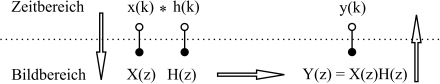
\includegraphics[width = 10cm]{psZ/SchematischezLoesungFaltung}
\caption{\label{pic:SchemaZLoesungFaltung} Schematische Darstellung zur Berechnung
der Faltungssumme mit Hilfe der z-Transformation.}
\end{center}
\end{figure}

\begin{example}
Das System ist durch
\[
    y(k) = x(k) -2x(k-1) + x(k-2)
\]
gegeben. Die z-Transformation führt auf eine z-Übertragungsfunktion
\[
    H(z) = 1-2z^{-1} + z^{-2}
\]
Für die Eingangsfolge:
\[
    x(k) = \delta(k) + 2\delta(k-1)  + 3\delta(k-2)  + 4\delta(k-3)  + 5\delta(k-4)
\]
ergibt sich die z-Transformierte zu
\[
X(z) = 1 + 2z^{-1} + 3z^{-2}+ 4z^{-3}+ 5z^{-4}
\]
Eine Polynommultiplikation führt zu der Ausgangs-z-Funktion
\[
Y(z) = X(z)H(z) = 1 -6 z^{-5} + 5 z^{-6}
\]
Damit ergibt sich für die Ausgangsfolge
\[
    y(k) = [1 \:\: 0 \:\: 0 \:\: 0 \:\: 0 \:\: -6 \:\: 5]
\]
bzw.
\[
    y(k) = \delta(k) - 6 \delta(k-5) + 5 \delta(k-6)
\]
\end{example}

\wichtig{Die Faltung wird in der z-Ebene zu einer Multiplikation}

\section{Pol-Nullstellenplan}
Nachdem die Äquivalenz der Impulsantwort mit der
z-Übertragungsfunktion $H(z)$ bekannt ist, ist es möglich, Systeme
besser zu analysieren. Dazu schauen wir uns zunächst die typische
Übertragungsfunktion an.
\begin{equation}\label{eq:Uebertragungsfunktion}
 H(z) = \frac{b_0 + b_1z^{-1} + b_2z^{-2}+ \cdots b_M z^{-M}
    }{1 + a_1z^{-1} + a_2z^{-2}+ \cdots a_N z^{-N}}
    = \frac{\displaystyle \sum_{i=0}^M b_iz^{-i}}
    {\displaystyle \sum_{i=0}^N a_i z^{-i}} \Mit a_0 = 1
\end{equation}
Wir nehmen an, dass der Zählergrad $M$ kleiner oder gleich dem
Nennergrad $N$ ist. Dies ist gleichbedeutend mit der Annahme, dass
es sich um ein kausales System handelt\footnote{Würde gelten $M>N$
könnte man durch Polynomdivision eine Übertragungsfunktion
erhalten, die aus einem simplen Polynom und einer gebrochen
rationalen Funktion mit $M\leq N$ besteht, wobei das Polynom ein
Polynom in $z$ und nicht in $z^{-1}$ wäre und somit bei einer
z-Rücktransformation auf einen nicht-kausalen Anteil führen
würde.}. Die Ordnung des Systems wird unter dieser Annahme durch $N$
angegeben. Im allgemeinen Fall definiert das Maximum von $N$ und $M$
die Ordnung des Systems.

Die gebrochen rationale Funktion können wir auch in der
äquivalenten Produktform schreiben, wenn uns alle Nullstellen, des
Zähler- und Nennerpolynoms bekannt sind. Wir werden für die
Nullstellen des Nenners ab jetzt den Begriff Polstellen bzw. Pol
verwenden, da an diesen Punkten, die Übertragungsfunktion
unendlich wird.

\begin{eqnarray}\label{eq:Uebertragungsfunktion:Produktdarstellung}
 H(z)
 & = & b_0 \frac{(z-n_0)(z-n_1)\cdots(z-n_{M-1})}{(z-p_0)(z-p_1)\cdots(z-p_{N-1})}\\
 & = & b_0 \frac{\displaystyle \prod_{i = 0}^{M-1}(z-n_i)}
 {\displaystyle \prod_{i = 0}^{N-1}(z-p_i)}
 \end{eqnarray}

Für reelle Koeffizienten $b_i$ und $a_i$ ergeben sich dabei immer
nur reelle Nullstellen oder konjugiert komplexe Paare.

\begin{example}
\begin{eqnarray}\nonumber
    H(z) & = & \frac{3+6z^{-1}+3z^{-2}}{1.0000   -1.7119 z^{-1} +   0.8100
    z^{-2}}\\\nonumber
    &=& 3\frac{(z+1)(z+1)}{(z-0.8560 - 0.2781j)(z-0.8560 +
    0.2781j)}\\\nonumber
    &=& 3\frac{(z+1)^2}{(z-0.9e^{j\frac{\pi}{10}})(z-0.9e^{-j\frac{\pi}{10}})}
\end{eqnarray}
\end{example}

Um bestimmte Eigenschaften zu verdeutlichen ist es oft sinnvoll,
die Pole und Nullstellen in der komplexen Ebene einzuzeichnen.
Dabei werden Nullstellen durch ein o und Pole durch ein x
markiert. Für das Beispiel ergibt sich der folgende
Pol-Nullstellenplan, wobei ein eventuell vorhandener Skalierungsfaktor $b_0$
nicht berücksichtige wird. Der Pol- Nullstellenplan ist deshalb keine
vollständige Beschreibung eines LTI-Systems.
\begin{figure}[H]
\begin{center}
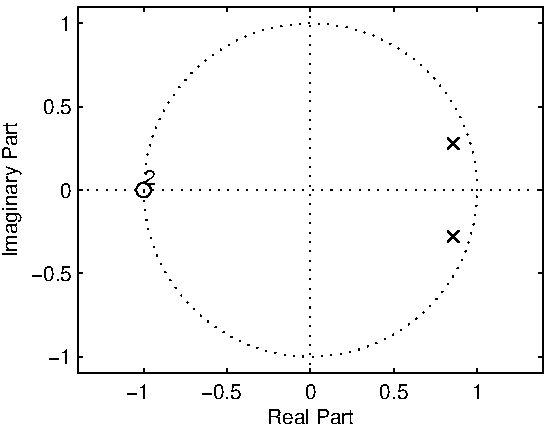
\includegraphics{psZ/PolNullstellenplan}
\caption{\label{pic:bspPolnullstellenplan}Pole und Nullstellen in
der komplexen Ebene.}
\end{center}
\end{figure}
Mehrfachnullstellen (oder auch Pole) werden durch eine zusätzliche
Zahl gekennzeichnet, hier die zwei für die doppelte Nullstelle bei
$z = -1$. Weiterhin ist der sog. Einheitskreis zu sehen, der den
Radius eins markiert und eine besondere Bedeutung hat, auf die wir
noch zu sprechen kommen.

Zur Verdeutlichung der Auswirkungen von Polen und Nullstellen
in der komplexen Ebene ist in Abbildung \ref{pic:PolNullstellenAuswirkung}
der Betrag der Übertragungsfunktion in Abhängigkeit vom Real und Imaginärteil
für das eben verwendete Beispiel gezeigt (Die Darstellung erfolgt logarithmisch.).
Zur Orientierung ist zusätzlich der Einheitskreis eingezeichnet.

\begin{figure}[H]
\begin{center}
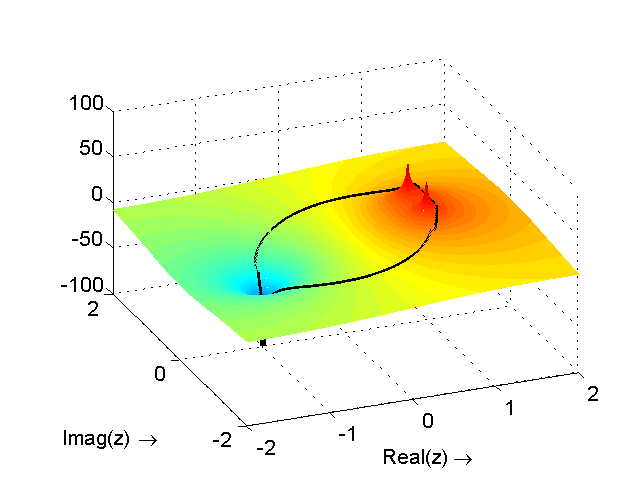
\includegraphics{psZ/PolNullstellenHz}
\caption{\label{pic:PolNullstellenAuswirkung}Übertragungsfunktion in der komplexen Ebene.}
\end{center}
\end{figure}

Der Einfluss der
beide Extremstellen auf den Betrag der Übertragungsfunktion ist auf der ganzen z-Ebene sichtbar.
Man erkennt sehr deutlich, wie die Pole zu einem unendlichen Betrag führen,
während die doppelte Nullstelle den Betrag zu Null werden lässt.

Welche Auswirkungen haben nun Polstellen auf die
Systemeigenschaften und insbesondere auf das Verhalten im
Zeitbereich. Grundsätzlich lassen sich die komplexen Pole immer
auch in der Polarschreibweise (Radius und Phase) angeben.

Betrachten wir jetzt ein System mit nur einem Pol (komplexwertiges
System)
\begin{equation}\label{eq:zTrafo:ErklaerungPolLage}
    H(z) = \frac{1}{1-re^{j\varphi}z^{-1}}
\end{equation}
Zurücktransfomiert in den Zeitbereich ergibt sich mit Hilfe der
Korrespondenztabelle
\begin{equation}\label{eq:zTrafo:ErklaerungPollageZeitbereich}
    h(k) = \gamma(k) r^k e^{j\varphi k}
\end{equation}
Interpretiert man Gleichung
\ref{eq:zTrafo:ErklaerungPollageZeitbereich} so ist zu erkennen,
dass die Impulsantwort aus einer komplexen Schwingung
($e^{j\varphi k}$) und einem Faktor besteht, der die Amplitude
ändert. Dieser Amplitudenfaktor wird als Einhüllende der komplexen
Schwingung bezeichnet. Die Frequenz der Schwingung ist durch den
Polwinkel $\varphi$ definiert und die Form der Einhüllenden durch
den Radius $r$. Für $r<1$ ergibt sich eine gedämpfte
Exponentialfunktion. Bei $r=1$ ist die komplexe Schwingung
ungedämpft und bei $r>1$ handelt es sich um eine aufklingende,
also mit der Zeit stärker werdende Schwingung.

Dies ist in der Abbildung \ref{pic:bspPollagen} nochmals
verdeutlicht. Die Pollage a) ist ein Pol auf der reellen Ache mit
einem Radius von $r = 0.96$\footnote{Die eingezeichneten Pollagen
sind zur Verdeutlichung skaliert.}. Die dazugehörige Schwingung
ist eine abklingende Exponentialfunktion ohne Schwingungsanteil.
Ist der Radius größer
eins (b) $r= 1.01$) ergibt sich eine aufklingende
Exponentialfunktion. Verschiebt man den Pol auf dem Radius $r=
0.96$ auf einen Polwinkel $\varphi = \pi/10$, so ergibt sich eine
exponentiell abklingende Schwingung (siehe c)). Bei einem Radius
größer eins, eine aufklingende Schwingung (d). Die Drehung ist bei
$\varphi = 3\pi / 4$ kaum noch zu erkennen (e), während die
Frequenz $\varphi = \pi$ erneut zu einer reellen Folge führt mit
wechselndem Vorzeichen. Der Radius entscheidet über das
Abklingverhalten (g,f). Die Drehrichtung wird durch die Pollage in
der oberen oder unteren Halbebene angegeben.

\begin{figure}[H]
\begin{center}
\includegraphics[width = 16cm]{psZ/PolLagen}
\caption{\label{pic:bspPollagen}Mögliche Pollagen und die
dazugehörigen komplexen Schwingungen im Zeitbereich (angelehnt an \cite{girod2013einfuhrung}).}
\end{center}
\end{figure}

Bei konjugiert komplexen Polpaaren heben sich durch die
gegensinnigen Drehrichtungen die Imaginäranteile auf und die
Impulsantwort $h(k)$ ist rein reellwertig. Die ausgebildeten
Schwingungen entsprechen gedämpften oder aufklingenden
Cosinusfunktionen der Frequenz $\varphi$.

Es gilt für
konjugiert ($^{\ast}$) komplexe Polpaare:
\begin{equation}
    \frac{Az}{z-a} + \frac{A^{\ast}z}{z-a^{\ast}} \RueckTrans 2|A||a|^k\cos(arg\{a\}k + arg\{A\})\gamma(k)
\end{equation}
$arg\{x\}$ ist das Argument (Winkel) von der komplexen Zahl $x$.

\begin{example}
Ausgehend von dem System
\[
    H(z) = \frac{z^2}{(z-0.9e^{j\frac{\pi}{10}})(z-0.9e^{-j\frac{\pi}{10}})}
\]
ergibt sich für die Aufspaltung
\[
    H(z) = \frac{Az}{z-0.9e^{j\frac{\pi}{10}}} + \frac{A^{\ast}z}{z-0.9e^{-j\frac{\pi}{10}}}
\]
mit
\begin{eqnarray}
    A &=& (z-0.9e^{j\frac{\pi}{10}})\widetilde{H}(z)\Bigg|_{z = 0.9e^{j\frac{\pi}{10}}}\\
    & = & \frac{z}{z-0.9e^{-j\frac{\pi}{10}}}\Bigg|_{z = 0.9e^{j\frac{\pi}{10}}}\\
    & = & \frac{0.9e^{j\frac{\pi}{10}}}{0.9e^{j\frac{\pi}{10}}-0.9e^{-j\frac{\pi}{10}}}\\
    & = & -j\frac{e^{j\frac{\pi}{10}}}{2\sin \frac{\pi}{10}}
\end{eqnarray}
Die Impulsantwort ist also durch
\[
    h(k) = 2\cdot 1.618 \cdot 0.9^k \cos\left(\frac{\pi}{10}k +\left(-\frac{\pi}{2} + \frac{\pi}{10}\right)\right)\gamma(k)
\]
gegeben und wird in Abbildung \ref{pic:BspKonjKomplexPol} bis $k = 49$ gezeigt.
\begin{figure}[H]
\begin{center}
\includegraphics{psZ/BspKonjKomplexPole}
\caption{\label{pic:BspKonjKomplexPol}Beispiel der Impulsantwort eines Systems mit
konjugiert komplexen Polpaar.}
\end{center}
\end{figure}
\hspace{0.1mm}
\end{example}

\section{Stabilität}
Mit den Erklärungen für Abbildung \ref{pic:bspPollagen} ist die
Frage nach einem Stabilitätstest für kausale LTI-Systeme recht einfach zu
beantworten. Da alle Systeme mit Polradien größer eins
aufklingende Schwingungen erzeugen sind die dazugehörigen
Impulsantworten nicht endlich. Auf einen endlichen Impuls reagiert
das System mit einer unendlichen Ausgangsgröße. Damit ist die
BIBO-Bedingung nicht mehr erfüllt.
\wichtig{Stabile, kausale
Systeme haben nur Pole innerhalb des Einheitkreises.}
\wichtig{Quasistabil sind Systeme mit einfachen Polen auf dem Einheitskreis}

Allgemein lässt sich sagen, dass Systeme deren z-Konvergenzgebiet den Einheitskreis
mit einschließen stabil sind. Betrachtet man noch einmal die
Beispiele für z-Transformation und des dazugehörigen Konvergenzgebietes
auf Seite \pageref{Bsp:z_TrafoUndROC}, so wird
deutlich, dass die kausale Folge ein stabiles System darstellt, während die
nicht-kausale Folge instabil ist. Man kann dies auch daran erkennen, dass
die Folge mit wachsendem $k$ größer wird.

Für LTI-Systeme ergibt sich als Kriterium für die BIBO-Stabilität.
\begin{equation}\label{eq:BIBO_INTEGRAL}
    \int_{-\infty}^{\infty} |h(t)|^2 dt < \infty
\end{equation}
bzw. für diskrete Systeme gilt
\begin{equation}\label{eq:BIBO_Diskret}
    \sum_{k = -\infty}^{\infty}|h(k)|^2 < \infty
\end{equation}

\subsection{Stabilität eines Systems 2. Ordnung}
Systeme zweiter Ordnung sind in der digitalen Signalverarbeitung
ein wichtiger Grundbaustein. Es ist deshalb interessant allgemein
die Stabilitätsbedingungen zu berechnen.
Das System ist durch
\begin{equation}
    H(z)=\frac{1}{1+a_{1}z^{-1}+a_{2}z^{-2}}
\end{equation}
gegeben. Um die Polstellen des Polynoms zu berechnen, muss
\begin{equation}
    z^{2}+a_{1}z+a_{2}=0
\end{equation}
\zB mit der bekannten pq-Formel
\begin{eqnarray}
    z_{1}& = &-\frac{a_{1}}{2}+\sqrt{\frac{a_{1}^{2}}{4}-a_{2}}\\
    z_{2}& = &-\frac{a_{1}}{2}-\sqrt{\frac{a_{1}^{2}}{4}-a_{2}}
\end{eqnarray}
berechnet werden.

Die Stabilität ist immer für einen Betrag von $\left|z\right|<1$
gesichert. Welche Bedingungen müssen für die Koeffizienten
$a_1$ und $a_2$ gelten?

Zur Lösung nehmen wir zunächst eine Fallunterscheidung vor:
\begin{enumerate}
    \item{ Für die komplexwertige Lösung $a_{2}>\frac{a_{1}^{2}}{4}$
    ergibt sich durch die Nebenbedingung, dass man $\sqrt{-1} = j$
    vor die Wurzel ziehen kann und sich somit die Vorzeichen umdrehen.
    \begin{equation}
    z=-\frac{a_{1}}{2} \pm j \sqrt{a_{2}-\frac{a_{1}^{2}}{4}}
    \end{equation}
    Berechnet man den Betrag ergibt sich
    \begin{eqnarray}
    \left|z\right| & = & \sqrt{\frac{a_{1}^{2}}{4}+a_{2}-\frac{a_{1}^{2}}{4}}\\
    & = & \sqrt{a_{2}}
    \end{eqnarray}
    Da für ein stabiles System $\left|z\right|<1$ gelten muss, gilt
    als erste Bedingung, dass auch $a^2_{2}<1$ sein muss}

    \item{Für die reelwertige Lösung gilt $a_{2}<\frac{a_{1}^{2}}{4}$:\\
    Es ergibt sich damit die folgende Ungleichung.
    \begin{equation}
        -1 < -\frac{a_{1}}{2} \pm \underbrace{\sqrt{\frac{a_{1}^{2}}{4}-a_{2}}}_{>0} < 1
    \end{equation}
    Löst man diese Ungleichung zunächst für das erste Ungleichheitszeichen und nutzt
    die negative Lösung, da diese ja immer kleiner ist als die positive Lösung
    \begin{equation}
        -1<-\frac{a_{1}}{2} - \sqrt{\frac{a_{1}^{2}}{4}-a_{2}}
    \end{equation}
    ergibt sich (zunächst Multiplikation mit -1, danach quadrieren und ausrechnen)
    \begin{eqnarray}
        -1+\frac{a_{1}}{2} & < & - \sqrt{\frac{a_{1}^{2}}{4}-a_{2}}\\
        \left(1-\frac{a_{1}}{2}\right)^{2}& > & \frac{a_{1}^{2}}{4}-a_{2}\\
        1-2\frac{a_{1}}{2}+\frac{a_{1}^{2}}{4}& > & \frac{a_{1}^{2}}{4}-a_{2}\\
        1-a_1 &  >  & -a_2 \\
        a_{1} & <  & a_{2}+1
    \end{eqnarray}
    Für das zweite Ungleichheitszeichen gilt entsprechendes. Die zweite
    Bedingung lautet
    \begin{equation}\label{eq:SOS:Ungleichung2}
    a_1 > -a_2 -1
    \end{equation}
    }
\end{enumerate}
Fasst man diese Bedingungen zusammen, ergibt sich für $a_2$ eine
untere Grenze von $a_2>-1$.
Alles zusammen beschreibt ein Dreieck, dass als Stabilitätsdreieck
für kausales System 2. Ordnung bezeichnet wird (siehe Abbildung \ref{pic:Stabilddreieck}).

\begin{figure}[H]
\begin{center}
\includegraphics{psZ/Stabildreieck}
\caption{\label{pic:Stabilddreieck}Stabilitätsdreieck für Systeme zweiter Ordnung mit
den Koeffizienten $a_1$ und $a_2$.}
\end{center}
\end{figure}
\compileif{bBook}
{
\section{Matlab und z-Transformation}
\tbd{poly roots Anwendung erklären\\ zplane als Anzeige Tool }

}

\section{Übungen}
\subsection{Wiederholung des Stoffes und einfache Rechenaufgaben}
\begin{enumerate}
    \item Welche Bedingungen müssen gelten, damit ein LTI-System stabil ist?
    \item Welche Beschreibungen eines LTI-Systems kennen Sie?
    \item Warum ist die Angabe der z-Transformationsfunktion nicht ausreichend?
    \item \label{Aufg:zTrafo:Stabilitaet}Testen Sie die folgenden LTI - Systeme auf Stabilität:
    \begin{enumerate}
        \item $y(k) = -2 y(k-1) + 1.5 x(k) - 2x(k-1)$
        \item $y(k) =  2.5 x(k-1) + 1.83 y(k-1)  - 0.99y(k-2)$
        \item $y(k) =  0.3 x(k) + 07 x(k-1) + 1.9812 y(k-1)   - 1.0201 y(k-2)$
    \end{enumerate}
    \item{Zeigen Sie, dass die Ungleichung \ref{eq:SOS:Ungleichung2} gilt.}
\end{enumerate}
\subsection{Aufgaben (Auf Klausurniveau)\label{Aufg:zTrafo:Klausurniveau}}
\begin{enumerate}
    \item Zeigen Sie, dass die z-Transformation eine lineare Transformation ist, indem
    Sie den Linearitätstest durchführen.
    \item \label{Aufg:zTrafo:zTrafo}Welchen Wert hat das folgende System nach 50 Schritten. Geben Sie die direkte
    Berechnungsmethode an. Ist das System BIBO-stabil?\\
    $y(k) = \sqrt(2) y(k-1) -  y(k-2) + 0.5 \delta(k)$
    \item Sind die folgenden Systeme kausal, stabil, linear und
    zeitinvariant? Begründen Sie ihre Antwort (auch wenn Sie keine Aussage machen können) mathematisch oder
    textuell (16)!
    \begin{enumerate}
        \item $y(k) = 0.5 y(k-1) - 0.3 y(k-2) k + 0.4 x(k) - 0.5
        x(k-1)x(k-2)$
        \item $y(k+1) = 1.1 y(k-1) - 0.5 x(k+1) + 0.3 x(k) - 0.5
        x(k-1)$
        \item $y(k+1) = 2x(2k-k) - y(k+1) + 4 x(k-2) + 1.8 y(k-1)$
        \item $y(k) = 0.3 x(k) + 0.6x(k-1) - 0.7 x(k-2)y(k-2) + x(2k-2)$
    \end{enumerate}
    \item Ist das folgende Systeme kausal, stabil, linear und
    zeitinvariant? Begründen Sie ihre Antwort mathematisch oder
    textuell! Falls Sie keine Aussage treffen können, begründen Sie auch dies!
    $y(k+1) - 2y(k+2) + \alpha x(k+2) + x(k+1) =  1.99 y(k)$\\
    Nehmen Sie an $\alpha = 2$ (8 Punkte). Für welche Bereiche von $\alpha$ (rein reell)
    ist das System stabil (Begründung)? (2 Punkte)
    \item Sind die beiden folgenden Systeme kausal, stabil, linear und
    zeitinvariant? Begründen Sie ihre Antwort mathematisch oder
    textuell! Falls Sie keine Aussage treffen können, begründen Sie auch dies!
    \begin{enumerate}
    \item $y(k) + \beta^2 y(k-2) + x(k-2) = 2 x(k) - 2x(k-2) - 1.9
    y(k-1)$.\\
    Zur Beantwortung der Frage nehmen Sie an $\beta = \sqrt{0.5}$ (8 Punkte).\\
    Für welche Bereiche von $\beta$ ist das System stabil bzw.
    instabil (4 Punkte).
    \item $2y(k) - 3.7x(-k-2)k -0.3y(k-3) = 10x(k-10)$. (8 Punkte)
    \end{enumerate}

\end{enumerate}

\compileif{bBook}
{
\subsection{Matlab-Aufgaben}
\begin{enumerate}
    \item Lösen Sie die Aufgabe \ref{Aufg:zTrafo:Klausurniveau}.\ref{Aufg:zTrafo:zTrafo} durch
    den Aufbau des Systems und Iteration.
    \item Programmieren Sie eine Funktion, die einen Pol-Nullstellenplan zeichnet und zusätzlich im
    Titel den $b_0$-Koeffizienten ausgibt. Nutzen Sie als Anhaltspunkt die {\tt zplane} Funktion von Matlab.
    Hinweis: Sie benötigen den {\tt axis} Befehl um eine quadratische Grafik aufzubauen (siehe help).
    Sie sollten die {\tt mpoles} Funktion nutzen, um Mehrfach Null- bzw. Polstellen herauszufinden.
    \item Schreiben Sie eine Funktion, die es ermöglicht Systeme durch eine grafische Eingabe mit der Maus
    zu definieren. Zeichnen Sie dazu den Einheitskreis in eine figure. Hinweis: Sie benötigen den
    {\tt ginput} Befehl für die Maus-Eingabe und {\tt axis}, um eine quadratische Grafik zu erzeugen.
\end{enumerate}
}
\subsection{Transfer-Leistung}
\begin{enumerate}
    \item Wie sieht das Konvergenzgebiet für endliche Folgen aus?
    \item
    \item
\end{enumerate}
%
\compileif{bZusammenfassung}
{
\section{Zusammenfassung}
Die wichtigen Erkenntnisse aus diesem Kapitel sind:
\begin{itemize}
    \item Die Systemfunktion ist eine vollständige Beschreibung eines LTI-Systems
    \item Die Systemfunktion ist die z-Transformierte der Impulsantwort
    \item Die Angabe der z-Transformation ist nur mit ROC vollständig.
    \item Das Pol-Nullstellendiagramm ist bis auf die Grundverstärkung $b_0$ eine
    vollständige Beschreibung eines LTI-Systems
    \item Die Stabilität eines kausalen LTI-Systems lässt sich
in der z-Ebene durch die Berechnung der Polradien einfach testen. Es muss gelten, dass
alle Radien kleiner eins sind. Für strikt nicht-kausale Systeme müssen alle Radien größer eins sein, um
ein stabiles System darzustellen.
    \item Bei Systemen zweiter Ordnung müssen um stabile kausale Systeme zu realisieren,
    die rekursiven Koeffizienten $a_1$ und $a_2$ im
    Stabilitätsdreieck liegen.
    \item Pol- bzw. Nullstellen reeller Systeme sind entweder reellwertig oder treten als
    konjugiert komplexe Polpaare auf.
\end{itemize}

}
%\section{Lösungen zu den Aufgaben}
%\subsection{Wiederholung des Stoffes und einfache Rechenaufgaben}
%\begin{enumerate}
%    \item Welche Bedingungen müssen gelten, damit ein LTI-System stabil ist?
%    \loesung{Für kausale Systeme müssen alle Polradien innerhalb des Einheitskreises liegen.}
%    \item Welche Beschreibungen eines LTI-Systems kennen Sie?
%    \loesung{Vollständige Beschreibungen sind: Differenzengleichung, Systemfunktion, Impulsantwort}
%    \item Warum ist die Angabe der z-Transformationsfunktion nicht ausreichend?
%    \loesung{Untescheidliche Folgen haben die gleiche z-Transformierte.}
%    \item \label{Aufg:zTrafo:Stabilitaet}Testen Sie die folgenden LTI - Systeme auf Stabilität:
%    \begin{enumerate}
%        \item $y(k) = -2 y(k-1) + 1.5 x(k) - 2x(k-1)$
%        \loesung{Nicht Stabil, Pol außerhalb}
%        \item $y(k) =  2.5 x(k-1) + 1.83 y(k-1)  - 0.99y(k-2)$
%        \loesung{stabil, siehe Stabilitätsdreieck}
%        \item $y(k) =  0.3 x(k) + 07 x(k-1) + 1.9812 y(k-1)   - 1.0201 y(k-2)$
%        \loesung{instabil, siehe Stabilitätsdreieck}
%    \end{enumerate}
%\end{enumerate}
%\subsection{Aufgaben (Auf Klausurniveau)\label{Aufg:zTrafo:Klausurniveau}}
%\begin{enumerate}
%    \item Zeigen Sie, dass die z-Transformation eine lineare Transformation ist, indem
%    Sie den Linearitätstest durchführen.
%    \loesung{Hmmm}
%    \item \label{Aufg:zTrafo:zTrafo}Welchen Wert hat das folgende System nach 50 Schritten. Geben Sie die direkte
%    Berechnungsmethode an. Ist das System BIBO-stabil?\\
%    $y(k) = \sqrt(2) y(k-1) -  y(k-2) + 0.5 \delta(k)$
%    \item Sind die folgenden Systeme kausal, stabil, linear und
%    zeitinvariant? Begründen Sie ihre Antwort (auch wenn Sie keine Aussage machen können) mathematisch oder
%    textuell (16)!
%    \begin{enumerate}
%        \item $y(k) = 0.5 y(k-1) - 0.3 y(k-2) k + 0.4 x(k) - 0.5
%        x(k-1)x(k-2)$
%        \item $y(k+1) = 1.1 y(k-1) - 0.5 x(k+1) + 0.3 x(k) - 0.5
%        x(k-1)$
%        \item $y(k+1) = 2x(2k-k) - y(k+1) + 4 x(k-2) + 1.8 y(k-1)$
%        \item $y(k) = 0.3 x(k) + 0.6x(k-1) - 0.7 x(k-2)y(k-2) + x(2k-2)$
%    \end{enumerate}
%    \item Ist das folgende Systeme kausal, stabil, linear und
%    zeitinvariant? Begründen Sie ihre Antwort mathematisch oder
%    textuell! Falls Sie keine Aussage treffen können, begründen Sie auch dies!
%    $y(k+1) - 2y(k+2) + \alpha x(k+2) + x(k+1) =  1.99 y(k)$\\
%    Nehmen Sie an $\alpha = 2$ (8 Punkte). Für welche Bereiche von $\alpha$ (rein reell)
%    ist das System stabil (Begründung)? (2 Punkte)
%    \item Sind die beiden folgenden Systeme kausal, stabil, linear und
%    zeitinvariant? Begründen Sie ihre Antwort mathematisch oder
%    textuell! Falls Sie keine Aussage treffen können, begründen Sie auch dies!
%    \begin{enumerate}
%    \item $y(k) + \beta^2 y(k-2) + x(k-2) = 2 x(k) - 2x(k-2) - 1.9
%    y(k-1)$.\\
%    Zur Beantwortung der Frage nehmen Sie an $\beta = \sqrt{0.5}$ (8 Punkte).\\
%    Für welche Bereiche von $\beta$ ist das System stabil bzw.
%    instabil (4 Punkte).
%    \item $2y(k) - 3.7x(-k-2)k -0.3y(k-3) = 10x(k-10)$. (8 Punkte)
%    \end{enumerate}
%
%\end{enumerate}
%
%\subsection{Matlab-Aufgaben}
%\begin{enumerate}
%    \item Lösen Sie die Aufgabe \ref{Aufg:zTrafo:Klausurniveau}.\ref{Aufg:zTrafo:zTrafo} durch
%    den Aufbau des Systems und Iteration.
%    \item Programmieren Sie eine Funktion, die einen Pol-Nullstellenplan zeichnet und zusätzlich im
%    Titel den $b_0$-Koeffizienten ausgibt. Nutzen Sie als Anhaltspunkt die \verb/zplane/ Funktion von Matlab.
%    Hinweis: Sie benötigen den \verb/axis/ Befehl um eine quadratische Grafik aufzubauen (siehe help).
%    Sie sollten die \verb/mpoles/ Funktion nutzen, um Mehrfach Null- bzw. Polstellen herauszufinden.
%    \item Schreiben Sie eine Funktion, die es ermöglicht Systeme durch eine grafische Eingabe mit der Maus
%    zu definieren. Zeichnen Sie dazu den Einheitskreis in eine figure. Hinweis: Sie benötigen den
%    \verb/ginput/ Befehl für die Maus-Eingabe und \verb/axis/, um eine quadratische Grafik zu erzeugen.
%\end{enumerate}
%
%\subsection{Transfer-Leistung}
%\begin{enumerate}
%    \item Wie sieht das Konvergenzgebiet für endliche Folgen aus?
%    \item
%    \item
%\end{enumerate}

\chapter{Spektren}
Wir haben bisher zwei Beschreibungsebenen für diskrete Signale und
Systeme kennen gelernt, den Zeitbereich mit der
Differenzengleichung und die z-Ebene. Häufig ist aber von
Interesse, wie sich die Signale und Systeme in Abhängigkeit von
der Frequenz verhalten. Diese Darstellung wird als Spektrum
bezeichnet. Dabei ist das Betragsverhalten (Betragsspektrum), also
ob und mit welcher Leistung eine Frequenz im Signal vorhanden ist
oder ob ein System eine bestimmte Frequenz verstärkt oder dämpft,
interessant. Das Phasenverhalten ist für viele Anwendungen von
sekundärer Bedeutung. Trotzdem kann insbesondere bei der
Beschreibung von Systemen das Phasenspektrum eine wichtige
Information darstellen.

\tbd{Motivationsbeispiel: Feedbackproblematik im Hörgerät oder bei
der Bühnenbeschallung. Analyse des Signals (Spektrum) ermöglicht
zu erkennen, bei welcher Frequenz die Störung auftritt. Nach der
Analyse kann bei dieser Frequenz ein System eingebaut werden, dass
die Übertragung dämpft. Durch den frequenzselektiven Eingriff wird
das Nutzssignal nur unwesentlich beeinflusst.}

\tbd{Aktives Beispiel wäre schön.}

Eine Möglichkeit das Verhalten bei einer bestimmten Frequenz zu
testen, ist, das LTI-System mit Signalen anzuregen die nur aus
einer Frequenz bestehen und dann die Veränderung am Ausgang zu
messen. Ein sehr gutes Eingangssignal um Betrag und Phase zu
bestimmen ist die ungedämpfte diskrete Exponentialschwingung
\begin{equation}\label{eq:Def:Euler}
    e^{j\Omega_0 k} = \cos(\Omega k)+j\sin(\Omega k)
\end{equation}
mit $\Omega_0 = 2 \pi f_0/ f_s$, wobei $f_0$ die Analysefrequenz und
$f_s$ die Samplingfrequenz angibt.

\hspace{1cm}\begin{minipage}{10cm}
{\bf Exkurs: Frequenzachsen in der DSV}
Manchmal ist es verwirrend in welcher Form Frequenzen in der
digitalen Signalverarbeitung angegeben werden. Die am häufigsten verwendeten Systeme
und ihre Äquivalenz als Achse und ihre Position auf dem Einheitskreis in der z-Ebene zeigt
Abbildung \ref{pic:FrequenzenDSV}.
\begin{figure}[H]
\begin{center}
\includegraphics{psSpek/FrequenzskalierungenExkurs}
\caption{\label{pic:FrequenzenDSV}Veranschaulichung der unterschiedlichen Frequenzbezeichnungen
in der DSV und ihre Position auf dem Einheitskreis in der z-Ebene.}
\end{center}
\end{figure}
\end{minipage}

Mit Hilfe der Faltung ergibt sich am Ausgang eines durch die
Impulsantwort beschriebenen Systems.
\begin{eqnarray}\label{eq:fTrafo:Bsp}
    y(k)& = &x(k)\ast h(k) = \sum_{\kappa = -\infty}^{\infty} h(\kappa)
    e^{j\Omega_0(k-\kappa)}\\
    &= & \underbrace{e^{j\Omega_0 k}}_{\mbox{Eingangssignal}} \cdot
    \underbrace{\sum_{\kappa = -\infty}^{\infty} h(\kappa) e^{-j\Omega_0
    \kappa}}_{\mbox{Komplexer Multiplikator}}
\end{eqnarray}
Das heißt also, am Ausgang können wir eine Schwingung derselben
Frequenz messen, die nur in ihrer Phase und ihrem Betrag geändert
wird. Berechnen wir dieses Ausgangsverhalten für alle Frequenzen
erhalten wir das Spektrum. Auffällig bei LTI-Systemen ist, das
keine neuen Frequenzen entstehen. Dies ist eine typische
Eigenschaft von LTI-Systemen.

\wichtig{LTI-Systeme erzeugen keine neuen Frequenzen}

Bei Systemen wird die frequenzabhängige Veränderung des Betrages
und der Phase Übertragungsfunktion genannt und kann mit
\begin{equation}\label{eq:DTFD:Hin}
    H \jom = \sum_{k = -\infty}^{\infty} h(k) e^{-j\Omega k}
\end{equation}
berechnet werden. Diese Form ist eng verwandt mit der
Fourier-Transformation für analoge Signale und wird deshalb
Zeitdiskrete Fourier-Transformation ({\em Discrete Time
Fourier-Transformation (DTFT)}) genannt.

Vergleichen wir nun Gleichung \ref{eq:DTFD:Hin} mit der Definition
der z-Transformation, so erkennen wir, dass die DTFT die
z-Transformation für $z = e^{j\Omega}$ darstellt und somit genau
den Einheitskreis in der z-Ebene beschreibt. Wir können also
direkt am Einheitskreis das frequenzabhängige
Übertragungsverhalten von Systemen ablesen. Dies gilt analog
natürlich auch für Signale.

Kennen wir also die z-Transformation eines Systems können wir auch
sofort die Übertragungsfunktion angeben. Betrachten wir
beispielsweise das System $y(k) = x(k) + x(k-1)$, dann ergibt
$e^{j\Omega}$ in die z-Transformierte eingesetzt
\begin{equation}\label{eq:fTRafo:Bsp:zTrafoFTrafo}
    H \jom = 1+z^{-1} \Big|_{z = e^{j\Omega}} = 1+e^{-j\Omega}
\end{equation}
Durch Umformungen erhalten wir.
\begin{eqnarray}\label{eq:fTrafo:BspUebrtragungF}
   e^{j\Omega / 2} H \jom &= & e^{j \Omega / 2}+e^{-j\Omega / 2}\\
   & = & \underbrace{2 \cos(\Omega / 2)}_{\mbox{Betrag, wenn $|\cdot|$}}
   \underbrace{e^{-j\Omega / 2}}_{\mbox{Phase}}
\end{eqnarray}

Die komplexwertige Darstellung mit Real und Imaginärteil ist dabei
zur Veranschaulichung und Interpretation nicht geeignet. Statt
dessen wird das komplexe Signal meist in den Betragsfrequenzgang,
d.h, eine Darstellung von $|H \jom|$ über der Frequenz und den
Phasengang, eine Darstellung des Arguments von $H \jom$,
aufgeteilt, wobei beim Betrag oder dem Betragsquadrat auch häufig
eine logarithmische Darstellung gewählt wird

\section{Einfluss der Pole und Nullstellen auf die Übertragungsfunktion}
Um den Einfluss der Pole und Nullstellen auf die
Übertragungsfunktion abzuschätzen, schauen wir uns zunächst noch
einmal die Abbildung \ref{pic:PolNullstellenAuswirkung} an. Bei
dieser Abbildung ist $|H \jom|^2$ logarithmisch dargestellt. Der
Betragsfrequenzgang der DTFT kann direkt aus dem enstehenden
''Gebirge'' abgelesen werden, wenn wir den Einheitskreis vom
Winkel $0$ bis $\pi$ umlaufen. Der Pol bei $\pi/10$ verursacht
eine Verstärkung auf dem Einheitskreis. Ein Pol direkt auf dem
Einheitskreis würde zu einer unendlichen Verstärkung führen.
Sobald der Winkel größer wird als $\pi/10$ nimmt die Verstärkung
ab. Ab einem Winkel von $\pi/2$ werden die Nullstellen dominant,
die dazu führen, dass sich der Betragsfrequenzgang null nähert und
die Null bei genau $\pi$ erreicht. Auf dem unteren Halbkreis geht
zunächst der Einfluss der Nullstelle zurück und der konjugiert
komplexe Pol bei $-\pi/10$ gewinnt an Einfluss. Bei $\Omega =
2\pi$ sind wir erneut bei $\Omega = 0$. Der Betragsfrequenzgang
wiederholt sich also periodisch in $2\pi$ für diskrete Signale.
Dies ist auch direkt aus der Beziehung
\begin{equation}\label{Eq:Spek:PeridozitaetsERklaerung}
    e^{j\Omega k} = e^{j(\Omega +2\pi n) k} \quad \forall \quad n \in \mathbb{N}
\end{equation}
zu sehen.

Eine direkte Berechnung des Betrag- und Phasenganges aus den Polen
und Nullstellen ist ebenfalls möglich. Um das zu veranschaulichen
ist in Abbildung \ref{pic:SpecPolNullstellen} ein System zweiter
Ordnung in der z-Ebene mit den zwei Polen und den zwei Nullstellen
gezeigt.
\begin{figure}[H]
\begin{center}
\includegraphics{psSpek/UebertragPolNullstellen}
\caption{\label{pic:SpecPolNullstellen}Skizze zur
Veranschaulichung des Einflusses von Polen und Nullstellen auf die
Übertragungsfunktion $H \jom$.}
\end{center}
\end{figure}

Um den Betrag des Frequenzganges an der Stelle $P$ zu berechnen,
müssen die Abstände der Pole und Nullstellen zu diesem Punkt $A_1,
A_2,B_1,B_2$ bekannt sein. Er ergibt sich
\begin{equation}\label{eq:spec:EInfacheBetragsrechnung}
    \left|H \jom\right|\Big|_{e^{j\Omega} = P} = |b_0| \frac{B_1 B_2}{A_1
    A_2}.
\end{equation}
Zusätzlich hat der Koeffizient $b_0$ einen Einfluss, der aber aus
dem Pol-Nullstellenplan nicht ersichtlich ist.

Die Phase an diesem Punkt kann durch
\begin{equation}\label{eq:spec:EenfachePhasenrechnung}
    \arg\left\{H \jom \right\}\Big|_{e^{j\Omega} = P} = -\arg\{b_0\}  + \beta_1 + \beta_2
    - \alpha_1 - \alpha_2
\end{equation}
berechnet werden. Da $b_0$ für reellwertige Systeme ebenfalls
reell ist, kann der Term $\arg\{b_0\}$ auch weggelassen werden, bzw.~führt bei negativem
$b_0$ zu einer Phasendrehung von $\pi$.

Für allgemeine Systeme mit einem Zählergrad $M$ und einem
Nennergrad $N$ ergibt sich \cite{KK98}.
\begin{equation}\label{eq:SpektrumBetragAllg}
    \left|H \jom\right| = |b_0| \frac{\displaystyle \prod_{i = 0}^{M-1} \sqrt{1-2|n_i|\cos(\Omega-\arg\{n_i\})+|n_i|^2}}
    {\displaystyle \prod_{i = 0}^{N-1}\sqrt{1-2|p_i|\cos(\Omega-\arg\{p_i\})+|p_i|^2}}
\end{equation}
bzw. für die Phase
\begin{eqnarray}\label{eq:SpektrumPhaseAllg}
    \arg\left\{H \jom\right\} &=& (M-N)\Omega - \arg\{b_0\} \\\nonumber
    && - \sum_{i = 0}^{M-1}\arctan\left\{\frac{\sin \Omega-|n_i|\sin(\arg\{n_i\})}{\cos \Omega-|n_i|\cos(\arg\{n_i\})}
    \right\}\\\nonumber
    && +\sum_{i = 0}^{N-1}\arctan\left\{\frac{\sin \Omega-|p_i|\sin(\arg\{p_i\})}{\cos \Omega-|p_i|\cos(\arg\{p_i\})} \right\}
\end{eqnarray}

\tbdb{Hier fehlt ein Beispiel, dass in Matlab erklärt wird}

\tbd{Phase muss noch deutlich besser erklärt werden, außerdem scheint die Phasenformel falsch zu sein}

Eine Interpretation führt zu den Schlüssen:
\begin{itemize}
    \item Je näher ein Pol am Einheitkreis liegt umso größer ist
    sein Einfluss auf die Übertragungsfunktion
    \item Eine Nullstelle auf dem Einheitskreis führt zu einem
    Phasensprung um $\pi$.
    \item Systeme, bei denen alle Nullstellen im inneren des 
    Einheitskreises liegen, heißen minimalphasig.
    \item Pole oder Nullstellen im Ursprung verändern nur die Phase, aber nicht den
    Betrag der Übertragungsfunktion.
    \item Nullstellen die am Einheitskreis gespiegelt werden $r_{out} = 1/r_{in}$,
    führen nur zu einer Veränderung der Grundverstärkung des Betrages der
    Übertragungsfunktion aber nicht zu einer Veränderung der Form. Gleichzeitig
    wird aber die Phase so verändert, dass sie um über $180^{\circ}$ dreht und das
    resultierende System nicht mehr minimalphasig ist.
    \item Systeme bei denen die Nullstellen an den Positionen der am Einheitskreis
    gespiegelten Pole liegen
    \begin{equation}\label{eq:AllpassGrundlagenFormel}
    n_{i_0} = \frac{1}{p_{i_{\infty}}}
    \end{equation}
    heißen Allpasssysteme, da der Betrag
    für alle Frequenzen konstant bleibt. Nur die Phase wird
    verändert und dreht um $N \pi$, wobei $N$ die Ordnung
    des Systems angibt.
\end{itemize}

\section{Diskrete Fourier-Transformation\label{sec:DFT}}
Zur Frequenzanalyse ist bisher nur die DTFT bekannt. Aber diese
Transformation kann nicht auf einem Computer umgesetzt werden, da
das resultierende Spektrum nicht diskret ist. Außerdem benötigt
man unendlich viele Eingangswerte um das Spektrum zu berechnen.
Deshalb wird in einem ersten Schritt die Anzahl der genutzten
Abtastwerte auf $N$ beschränkt. Man könnte dies auch so
interpretieren, dass die unendliche Folge des Signals mit einer
Rechteckfolge der Höhe eins und der Länge N multipliziert wird. Da
außerhalb des Eins-Bereichs alle Multiplikationen zu Null werden,
können auch die Summengrenzen verändert werden.

Diese Rechteckfolge werden wir im weiteren mit Fenster oder {\em
Window} bezeichnen, da es aus der Folge nur einen Ausschnitt
zeigt, in Anlehnung an ein Glasfenster , das uns nur einen
Ausschnitt der Wirklichkeit zeigt (siehe Abbildung
\ref{pic:DFT_FensterMult}). Die Länge $N$ nennen wir Blockgröße,
da nur noch ein Block an Daten verarbeitet wird.

\begin{figure}[H]
\begin{center}
\includegraphics{psSpek/DFT_FensterMultiplikation}
\caption{\label{pic:DFT_FensterMult}Veranschaulichung der Wirkung
einer Rechteck-Fensterfunktion der Länge $N = 16$.}
\end{center}
\end{figure}

Das resultierende Spektrum ist aber immer noch kontinuierlich.
Durch die periodische Wiederholung des Spektrums ist es aber
ausreichend nur den Bereich von $0 \leq \omega\leq 2\pi $ genauer
zu betrachten. Um jetzt eine diskretes Spektrum zu erhalten,
unterteilen wir das Spektrum in $N$ gleichförmige
Abschnitte\footnote{Man kann auch eine andere Anzahl verwenden,
aber $N$ führt zu besonders effizienten Lösungen.}.

Die DTFT geht damit in
\begin{equation}\label{eq:DFTHin:Def}
    X(n) = X\left(e^{j 2 \pi n / N}\right) = \sum_{k = 0}^{N-1}x(k) e^{-j 2 \pi n k /N}
\end{equation}
über.

Umgekehrt ist es natürlich auch möglich, aus den $N$
Spektralwerten auch auf die Folge zurück zuschließen. Die
Rücktransformation enthält zusätzlich noch einen Normierungsterm
$N$ und unterscheidet sich sonst nur in dem Vorzeichen der
e-Funktion.
\begin{equation}\label{eq:DFTRueck:Def}
    x(k) = \frac{1}{N} \sum_{n = 0}^{N-1}X(n) e^{j 2 \pi n k /N}
\end{equation}

Das Transformationspärchen \ref{eq:DFTHin:Def} und
\ref{eq:DFTRueck:Def} werden als diskrete Fourier-Transformation
(DFT), bzw.\ inverse DFT (IDFT) bezeichnet.


\section{Eigenschaften}
\subsection{Zusammenhang DTFT und DFT}
Wir haben, um von der exakten Darstellung des Spektrums mittels
DTFT auf die computerlösbare DFT zu kommen, zwei Veränderungen
vorgenommen und natürlich spiegeln sich diese Veränderungen auch
im Ergebnis wieder. Wir müssen also versuchen, die Veränderungen
zu analysieren, um sicher zu sein, dass die DFT zumindest eine
Näherung der DTFT ist.

Zunächst ist es interessant die vorgenommene Diskretisierung im
Frequezbereich zu untersuchen. Im Grunde genommen haben wir das
Spektrum abgetastet. Die Konsequenz der Abtastung kennen wir
bereits aus der normalen Abtastung im Zeitbereich. Es kommt zu
einer periodischen Wiederholung des Spektrums. Die Abtastung im
Frequenzbereich führt zu einer periodischen Wiederholung im
Zeitbereich. Wenn man also ein Signal analysiert und zurück
transformiert ergibt sich eine periodische Wiederholung. Auch hier
gibt es eine andere Interpretationsmöglichkeit. Bei der
Analyse von periodischen Signalen mittels Fourier-Reihen ergeben
sich diskrete Spektren. Ein diskretes Spektrum führt im
Umkehrschluss also zu einer periodischen Zeitfunktion, wobei bei
der DFT die Periode genau $N$ ist (siehe Abbildung
\ref{pic:DFT_SignalPeriode}).

\begin{figure}[H]
\begin{center}
\includegraphics{psSpek/DFT_SignalPeriodizitaet}
\caption{\label{pic:DFT_SignalPeriode}Veranschaulichung der
erzwungenen Signal-Periodizität durch die DFT.}
\end{center}
\end{figure}

Der Einfluss der Fenster-Funktion lässt sich zunächst nur durch
die DTFT beschreiben. Es ist bekannt, dass eine Faltung im
Zeitbereich zu einer Multiplikation im Bildbereich
(Frequenzbereich) führt. Das Umgekehrte gilt aber auch. Eine
Multiplikation im Zeitbereich, und die Nutzung des Fensters ist
eine Multiplikation, führt im Frequenzbereich zu einer Faltung der
Spektren, wobei die Faltung hier kontinuierlich als Integral zu
definieren ist, da wir ja ein kontinuierliches periodisches
Spektrum haben.
\begin{equation} \label{eq:SpektrumBegrenzterFolgen}
    H \jom \Big|_{0 \leq n \leq N} = \int_{\theta = -\pi}^{\pi} H
    (e^{j\theta}) H^{W}(e^{j(\Omega - \theta)})d\theta
\end{equation}
wobei $H^{W}$ die Übertragungsfunktion der Fensterfunktion ist.

Für das Rechteckfenster ergibt sich das Spektrum, indem
wir zunächst die z-Transformation der Fensterfolge $w(k)$ ansetzen
Es gilt:
\[
    H^{W}(z) = \sum_{k = -\infty}^{\infty} w(k) z^{-k} = \sum_{k = 0}^{N-1} z^{-k}
\]
Durch einsetzen von $z = e^{j\Omega}$ ergibt sich das Spektrum
\[
    H^{W}(z)\Big|_{z = e^{j\Omega}} = \sum_{k = 0}^{N-1} e^{-j\Omega k}
\]
mit der Formel der endlichen geometrischen Reihe\footnote{
\[
    1+x + x^2 + \cdots + x^{N-1} = \frac{1-x^N}{1-x}
\]}
erhält man das Spektrum der Rechteckfunktion:
\begin{eqnarray}
    H^{W}\jom & = & \frac{1-e^{-j\Omega N}}{1- e^{-j\Omega}}\\
    & = & \frac{e^{-j\Omega N/2} \overbrace{(e^{j\Omega N/2}- e^{-j\Omega N/2})}^{2j\sin(\Omega N/2)}}
    {e^{-j \Omega/2}\underbrace{(e^{j \Omega/2}- e^{-j\Omega/2})}_{2j\sin(\Omega/2)}}\\
    & = & e^{-j(N-1)\Omega/2}\frac{\sin\left(N \Omega/2
\right)}{\sin\left(\Omega/2 \right)}
\end{eqnarray}
Der vordere Teil dieser Funktion entspricht einer linearen
Phasenverschiebung. Der zweite Teil mit den Sinustermen stellt
eine sogenannte Dirichlet-Funktion dar. Der Betrag dieser Funktion ist in
Abbildung \ref{pic:DirichletFkt} gezeigt.

\begin{figure}[H]
\begin{center}
\includegraphics[width = 10cm]{psSpek/DirichletFkt}
\caption{\label{pic:DirichletFkt}Betrag von $H^{W}\jom$ für $N = 16$.}
\end{center}
\end{figure}

\begin{example}
DTFT und DFT bei einer Cosinus-Schwingung\\
Um die Unterscheide zwischen DTFT und DFT bei der Spektrumsberechnung
eines Cosinus müssen wir zunächst das Spektrum einer abgetasteten Cosinus-Schwingung berechnen:
\begin{eqnarray}
H \jom & = & \sum_{-\infty}^{\infty} \cos \left(k \Omega_0  \right) e^{-j\Omega k}\\
       & = & \sum_{-\infty}^{\infty} \frac{1}{2}\left( e^{j k \Omega_0} + e^{-j k \Omega_0}\right) e^{-j\Omega k}\\
       & = & \sum_{-\infty}^{\infty} \frac{1}{2} \left( e^{j k (\Omega_0-\Omega)} + e^{-j k (\Omega_0 + \Omega)}\right)\\
       & = & \sum_{-\infty}^{\infty} \frac{1}{2} e^{-j k (\Omega-\Omega_0)}
       + \sum_{-\infty}^{\infty} \frac{1}{2} e^{-j k (\Omega + \Omega_0)}\\
       & = & \frac{1}{2} \Dirac{\Omega - \Omega_0}
       + \frac{1}{2} \Dirac{\Omega + \Omega_0}
\end{eqnarray}
mit $\Omega = 2\pi f / f_s$.
Das heißt, das Spektrum des abgetasteten Cosinus hat nur zwei definierte
Frequenzwerte, an den Frequenzen $\Omega = \pm \Omega_0$.
\end{example}

Um den Einfluss der Annäherung durch die DFT zu veranschaulichen, begrenzen wir den
betrachteten Signalausschnitt auf $N$ Datenwerte. Dies führt wie in Gleichung
\ref{eq:SpektrumBegrenzterFolgen}
gezeigt zu einer Faltung mit dem Spektrum des Rechtecks. Durch die Siebeigenschaft
der $\delta$-Funktion ergibt sich
\begin{eqnarray}
    H \jom & = & \left(\frac{1}{2} \delta \left(\Omega - \Omega_0 \right)
       + \frac{1}{2} \delta \left(\Omega + \Omega_0 \right) \right) \ast H^{W} \jom \\
           & = & \frac{1}{2} H^{W} \left(e^{j(\Omega -\Omega_0 )}\right) +
                 \frac{1}{2} H^{W} \left(e^{j(\Omega + \Omega_0 )}\right).
\end{eqnarray}
Das Spektrum des Rechtecks wird also, um $\pm \Omega_0$ verschoben.
Abbildung \ref{pic:VerschobesRechteckSpektrum} zeigt
das resultierende Spektrum für $N = 16$ bei einer Grundfrequenz von 155Hz und einer Abtastrate von
$f_s = 1$kHz.

\begin{figure}[H]
\begin{center}
\includegraphics[width = 10cm]{psSpek/DFT_Cosinus}
\caption{\label{pic:VerschobesRechteckSpektrum}Spektrum (Rechts) einer abgetasteten Cosinus-Fkt., die auf
$N = 16$ Werte begrenzt wird (Links) ($f_s = 1 $kHz und $f_0 = 155$Hz).}
\end{center}
\end{figure}

Um nun das DFT-Spektrum zu berechnen ist zusätzlich die Abtastung im Frequenzbereich notwendig.
Dies hat implizit zur Folge, dass die Cosinusfolge periodisch wiederholt wird. Das
abgetastete Spektrum ist auf der linken Seite in
Abbildung \ref{pic:VerschobesRechteckSpektrumAbgetastet} zu sehen und die resultierende Folge
auf der rechten Seite.

\begin{figure}[H]
\begin{center}
\includegraphics[width = 10cm]{psSpek/DFT_CosinusSpektrum}
\caption{\label{pic:VerschobesRechteckSpektrumAbgetastet}Abgetastetes Spektrum (Links)
und die daraus resultierende periodisch fortgesetzte Cosinus-Fkt mit Sprungstellen (rechts).}
\end{center}
\end{figure}

Das resultierende Spektrum hat nicht das erwartete Maximum bei $f_0$, da $155Hz$ nicht
im Abtastraster einer 16 Punkte FFT bei einer Abtastrate von 1kHz liegt. Statt dessen ist
die Leistung des Cosinus über viele Abtastpunkte spektral verteilt. Dieser Effekt wird auch als
{\em Leakage} bezeichnet.

\tbd{Beispiele mit anderen Frequenzen, um zu zeigen, dass Dirichlet-Funktion abgetastet wird.}


\subsection{Symmetrien der DFT}
Eine der wichtigsten Symmetrien für die diskrete sowie für die
zeitdiskrete Fourier-Transformation (DFT und DTFT) ergibt sich für
reelle Signale. Aus den Eigenschaften der z-Transformation ist
deutlich, dass sich nur dann reelle Koeffizienten bei Signalen und
Systemen ergeben, wenn die Pole und Nullstellen konjugiert komplex
auftreten. Daraus ergibt sich, dass die Spektren reeller Signale
konjugiert komplex sind. Es ergibt sich also eine Symmetrie der
Spektren an der Null Hertz (Gleichstrom) Linie. Der Realteil ist
dabei achsensymmetrisch (gerade) und der Imaginärteil punktsymmetrisch (ungerade).
Diese Symmetrien ergeben sich auch, wenn Betrag und Phase
betrachtet werden. Der Betrag reeller Funktionen ist immer
achsensymmetrisch und die Phase punktsymmetrisch (siehe Abbildung \ref{pic:SymmetrienDFT})
\begin{figure}[H]
\begin{center}
\includegraphics[width = 10cm]{psSpek/SymmetriePlot}
\caption{\label{pic:SymmetrienDFT}Beispiel eines Frequenz- und Phasenverlaufs eines reellwertigen Systems.}
\end{center}
\end{figure}

Die Symmetrien lassen sich bei der Berechnung der DFT und IDFT
ausnutzen, da immer nur das halbe Spektrum berechnet werden muss,
während die andere Hälfte durch Spiegelung erzeugt werden kann.
Häufig kommt es vor, dass man im Spektralbereich etwas berechnet
und an der dazugehörigen Zeitfolge interessiert ist (zum Beispiel
beim Filterentwurf). Es reicht aus, für eine $N$-Punkte DFT,
$N/2+1$ Spektralwerte zu kennen. Man benötigt einen Wert mehr, da
die DFT für die höchste Frequenz bei $f_s/2$ nur einen
reellwertigen Koeffizienten besitzt. Die Kopievorschrift in Matlab
sieht dann wie folgt aus, wobei wir annehmen, die $N/2+1$ Werte
sind in \verb/H_halb/ gespeichert
\begin{verbatim}
H_voll = [H_halb conj(H_halb(end-1:-1:2))];
\end{verbatim}
Die Gegenprobe, ob alle Symmetrien richtig aufgebaut wurden, ist
das Überprüfen, ob nach der Rücktransformation eine rein
reellwertige Folge entsteht, wobei bei Matlab durch Rundungsfehler
immer die resultierende Variable komplex ist. Es ist deshalb immer
notwendig, den Betrag des Imaginäranteils zu überprüfen. Dieser
sollte sehr kleine Werte um $10^{-7}$ nicht überschreiten.

Wie lässt sich die Symmetriebedingung mathematisch zeigen?

Ausgehend von
\[
    X(n) = \sum_{k = 0}^{N-1} x(k) e^{-jkn2\pi/N}
\]
ergibt sich für die an der y-Achse gespiegelte Folge durch Variablensubstitution
\[
    X(-n) = \sum_{k = 0}^{N-1} x(k) e^{jkn2\pi/N}
\]
Konjugiert man dieses Signal ergibt sich
\begin{eqnarray}
    X^{\ast}(-n)  &  =  & \sum_{k = 0}^{N-1} \underbrace{x^{\ast}(k)}_{=x(k)\:\mbox{, da reell}}
    \underbrace{e^{-jkn2\pi/N}}_{\mbox{Beachte -}}\\
                  &  =  & X(n)
\end{eqnarray}

\subsubsection{Spektren reeller gerader Folgen}
Die Symmetriebedingung reeller gerader Folgen kann aus den vorherigen
Überlegungen geschlossen werden. Da gerade Funktionen achsensymmetrisch
sind, der Imaginärteil aber punktsymmetrisch, können wir schließen, dass
reelle, gerade Funktionen ein reelles, gerades Spektrum haben.

%\subsubsection{Weitere Symmetrien}

%\tbd{gerade / ungerade}

%Allgemein lässt sich für die einzelnen Teile eines komplexen Signals, die folgenden
%korrespondierenden Spektren finden.

%\tbd{Bild mit Transkreuz, siehe Girod}

\subsection{Rechenregeln}
\subsubsection{Linearität}
Die DFT ist eine lineare Transformation. Es gilt also das
Superpositionsprinzip:
\begin{equation}\label{eq:DFT:Linearitaet}
  a_1 x_1(k) + a_2 x_2(k) \HinTrans a_1 X_1(n) + a_2 X_2(n)
\end{equation}

\subsubsection{Faltung \label{sec:DFT:Faltung}}
Bisher haben wir bereits die Faltung bei der z-Transformation kennen gelernt und
den Übergang der Faltung in die Multiplikation in der z-Ebene. Dieser Zusammenhang
gilt auch für die DTFT, aber nicht so direkt für die DFT. Um das zu veranschaulichen,
kann ein einfaches Beispiel dienen. Gehen wir davon aus, dass wir eine Folge mit $N = 8$
Werten mit Hilfe der DFT in den Bildbereich transformieren. Wir erhalten 8 Frequenzpunkte.
Des Weiteren transformieren wir eine zweite Folge mit 8 Datenwerten. Wir erhalten
erneut 8 Spektralwerte. Multiplizieren wir diese beiden Spektren und führen eine
Rücktransformation durch, so besteht das Ergebnis auch aus 8 Werten im Zeitbereich.
Aus der Faltungsalgebra wissen wir aber, dass das Faltungsprodukt aus $L+M-1$
Elementen bestehen muss, in diesem Beispiel also 15 Datenwerte. Daraus folgt, dass die
Faltung nicht der Multiplikation mit den DFT-Spektralwerten entspricht.

Die Ursache hierfür ist in der implizierten Periodizität der DFT zu finden. Das DFT Spektrum
ist gerade nicht das Signal im betrachteten Zeitfenster, sondern ein Signal das periodisch
fortgesetzt ist. Die Multiplikation im Frequenzbereich führt deshalb auf eine Faltung dieser
periodisch fortgesetzten Sequenzen. Dies führt dazu, dass auch das Faltungsprodukt periodisch ist.
Man spricht deshalb von der zyklischen Faltung. Das Ergebnis kann sich vollständig von dem
gewünschten Ergebnis unterscheiden. Dies wird in Abbildung \ref{pic:BspZyklischeFaltung} demonstriert.
Die beiden Folgen (a,b) ergeben bei der Faltung im Zeitbereich die Folge c. Die Lösung mit Hilfe der
DFT führt auf die Folge d.

\begin{figure}[H]
\begin{center}
\includegraphics[width = 10cm]{psSpek/BspZyklischeFaltung}
\caption{\label{pic:BspZyklischeFaltung}Beispiel für zyklische Faltung. Die beiden Folgen (Bild a,b)
ergeben bei konventioneller Faltung Bild c. Bild d zeigt das Resultat für die direkte Faltung im
Frequenzbereich mit Hilfe der DFT.}
\end{center}
\end{figure}

Um die zyklischen Faltungsprodukte zu verhindern ist es notwendig Nullen an die
zu transformierenden Folgen anzuhängen ({\em Zero-Padding}) und eine entsprechend größere
Transformationslänge zu wählen. Dies führt dazu, dass die implizite Periodizität
die Nullen einschließt. Die Nullen verändern das Spektrum nicht, sondern nur die
Frequenzauflösung\footnote{Es enstehen keine genaueren Spektralwerte gegenüber der kurzen Folge.
Die Werte bei der höheren Frequenzauflösung könnten auch aus einer Interpolation
des Spektrums mit geringrer Auflösung gewonnen werden.}. Die Rücktransformation führt zu der
gewünschten Faltungsfolge, wobei durch die vorher eingebrachten Nullen
keine zyklischen Faltungsprodukte das Ergebnis
verfälschen. Bei dem obigen Beispiel würde sich das Ergebnis in Abbildung \ref{pic:BspZyklischeFaltung}c
ergeben, wenn an die Folgen a und b jeweils 8 Nullen angehängt werden und die DFT Länge auf 16
erhöht wird.

\tbd{Einfacheres Beispiel mit Rechteck und Dreiecksfunktionen, bei denen die
Wiederholungen eingezeichnet sind.}


\subsubsection{Theorem von Parseval}
Das Theorem von Parseval sagt aus, dass man die Energie eines Signals im Zeit, oder
im Frequenzbereich berechnen kann, bzw. dass die Leistung eines Signals im Zeit- und Frequenzbereich gleich ist.
Es gilt also für die DTFT:
\begin{equation}\label{eq:ParsevalDTFT}
    \sum_{k = -\infty}^{\infty} x^2(k) = \frac{1}{2\pi} \int_{-\pi}^{\pi} \left|X \jom \right|^2 d\Omega
\end{equation}
bzw. für die DFT
\begin{equation}\label{eq:ParsevalDFT}
    \sum_{k = 0}^{N-1} x^2(k) = \frac{1}{N}\sum_{n = 0}^{N-1} |X(n)|^2
\end{equation}



\subsection{Effiziente Implementierung}
Die DFT lässt sich durch Ausnutzung unterschiedlicher Symmetrien
sehr effizient berechnen. Um dies zu verdeutlichen, soll das sog.
{\em Decimation in Time}-Verfahren zur drastischen Reduktion der
benötigten Rechenleistung, genauer gezeigt werden. Andere
Verfahren können in der sehr umfangreichen Literatur zur
Entwicklung der sog. Fast Fourier Transform (FFT) gefunden werden
\cite{Coo90, KK98,OS99}

Um eine effiziente Realisierung zu finden, legen wir die Länge der
FFT so fest, dass sie eine 2er Potenz darstellt. Besonders häufig in der
Audio und Sprachsignalverarbeitung
genutzte FFT-Längen sind 256 , 512, 1024 und 2048.
Durch diese Forderung ist es möglich, die Folge in zwei Teilfolgen zu zerlegen, wobei
wir immer abwechselnd die Elemente der Folge, den jeweiligen neuen Teilfolgen zuordnen.
Es ergeben sich die Folgen $x(2k)$ und $x(2k+1)$ (siehe Abbildung \ref{pic:DecimationInTime}).

\begin{figure}[H]
\begin{center}
\includegraphics[width = 8cm]{psSpek/DecimationInTime}
\caption{\label{pic:DecimationInTime}Aufteilung einer Sequenz in zwei Teilsequenzen zur
Erklärung der FFT (Decimation in Time)}
\end{center}
\end{figure}

Die Konsequenzen für die DFT lassen sich nun wie folgt berechnen:
\begin{eqnarray} \nonumber
\sum_{k = 0}^{N-1} x(k) e^{-j 2 \pi n k /N} & = &
\sum_{k = 0}^{\frac{N}{2}-1} \underbrace{x(2k)}_{u(k)} e^{-j 2 \pi n 2k /N} +
\sum_{k = 0}^{\frac{N}{2}-1} \underbrace{x(2k+1)}_{v(k)} e^{-j 2 \pi n (2k+1) /N} \\\nonumber
& = & \underbrace{\sum_{k = 0}^{\frac{N}{2}-1}u(k) e^{-j 2 \pi n k /\frac{N}{2}}}_{U(n) \qquad \mbox {N/2 DFT}} +
e^{-j2\pi n /N} \underbrace{\sum_{k = 0}^{\frac{N}{2}-1}
v(k) e^{-j 2 \pi n k /\frac{N}{2}}}_{V(n) \qquad \mbox {N/2 DFT}}\\
X(n) & = & U(n) + e^{-j2\pi n /N} V(n)
\end{eqnarray}
Die N-Punkte DFT lässt sich also in zwei N/2-Punkte DFT zerlegen. Hierbei tritt jetzt das Problem auf,
dass die Folgen $U(n)$ und $V(n)$ nur bis $N/2$ definiert sind, da ja auch nur eine N/2 DFT durchgeführt wurde.
Die Lösung für dieses Problem ist durch die Periodizität der DFT aber sehr einfach zu umgehen, da sich das
Spektrum immer wiederholt.

Aber warum stellt es einen Vorteil dar, wenn man die DFT so zerlegen kann? Dazu müssen wir überlegen,
wie viele Multiplikationen notwendig sind um eine diskrete Frequenz zu berechnen. Es sind
$N$ komplexe Multiplikatinen nötig. Dieser Schritt muss für alle diskreten Frequenzen durchgeführt werden.
Die Berechnung des vollständigen Spektrums benötigt also $N^2$ Multiplikationen. Teilen wir die
Aufgabe in zwei Teilspektren benötigt man $2\left(\frac{N}{2}\right)^2$ + $N$ Multiplikationen für
den Drehfaktor vor $V(n)$. Im Vergleich ergeben sich \zB für $N = 8$ einmal 64 Multiplikationen
und für die aufgeteilten Spektren 40 Multiplikationen. Der Schritt der Aufteilung kann nun solange
wiederholt werden, bis die Folge nicht weiter aufgeteilt werden kann ($N = 2$). Zusätzlich
können einige Multiplikationen vernachlässigt werden, da $e^{j0} = 1$ ist. Eine
Reduktion auf $\frac{N}{2}\left( ld \frac{N}{2} \right)$ ist so möglich\footnote{ld bezeichnet den
Logarithmus zur Basis 2 (logarithmus dualis). }. Somit ergibt sich eine in der Rechenleistung
stark reduzierte DFT, die als {\em Fast Fourier Transform} (FFT) bekannt ist\footnote{In Matlab wird
die DFT durch den Befehl FFT aufgerufen.}.

\section{Spezielle Signale und ihre Spektren}

\subsubsection{Spektrum für $\delta(k)$}
Berechnet man die DTFT für den $\delta$-Impuls ergibt sich
\begin{equation}\label{eq:SpektrumDeltaImpuls}
    X \jom = \sum_{k = -\infty}^{\infty} \delta(k)e^{-jk \Omega} =e^{-j0 \Omega} = 1,
\end{equation}
da der $\delta$-Impuls ausschließlich an der Stelle $k = 0$ definiert ist.
Das Betrag des Spektrums ist also eins für alle Frequenzen und die Phase ist null
für alle Frequenzen.

\subsubsection{Spektrum für $\delta(k-k_0)$}
Der um $k_0$ verschobene $\delta$-Impuls führt zu einem etwas anderem Spektrum
\begin{equation}\label{eq:SpektrumDeltaImpuls}
    X \jom = \sum_{k = -\infty}^{\infty} \delta(k-k_0)e^{-jk \Omega} =e^{-jk_0 \Omega}.
\end{equation}
Das Spektrum ist im Betrag ebenfalls Eins für alle Frequenzen, aber die Phase des Signals
wird linear abhängig von der Frequenz verändert, wenn ein $\delta(k)$ ein System darstellt

%\subsubsection{Spektrum für $\gamma(k)$}

%\tbd{Nachschlagen}

\section{Weitere Fensterfunktionen und deren Eigenschaften}
Wir haben gesehen, dass die DFT für eine zeitlich beschränkte
Funktion auch als Multiplikation mit einer Fensterfunktion
interpretiert werden kann. Dieses Fenster hatte einen deutlichen
Einfluss auf das dargestellte Spektrum. Zur Beschreibung der
Eigenschaften des Fensters im Frequenzbereich wird häufig die
spektrale Auflösung des Maximums zu den 3dB Punkten verwendet.
Weiterhin ist eine interessante Größe, welche Höhe die nächsten
Maxima haben (Betrag). Für das Rechteckfenster sind diese beiden
Größen durch $2pi/N$ und $\approx 13$dB gegeben. Etwas anders sieht
dies bei anderen Fensterfunktionen aus (siehe Abbildungen
\ref{pic:HannWindow} - \ref{pic:KaiserFenster2}).
\begin{figure}[H]
\begin{center}
\includegraphics[width = 11cm]{psSpek/RechteckWindow}
\caption{\label{pic:RectWindow}Zeitliche und spektrale Eigenschaft
des Rechteckfensters}
\end{center}
\end{figure}

Als Ursache für das verschmieren im Frequenzbereich wurde die
Faltung mit der Fensterfunktion genannt. Die Ursache im
Zeitbereich hierfür war das abrupte Abschneiden, dass durch die
angenommene zirkulare WIederholung zu einem nicht-repräsentativen
Ausschnitt führte. Deshalb ist eine Design-Idee für andere Fenster
eine möglichst weiche Ausblendung zu den Rändern zu ermöglichen.
Fenster die diese Eigenschaft besitzen können zum Beispiel durch
Cosinusfunktionen realisiert werden.

Eine generalisierte Version ergibt sich dabei zu
\begin{equation}\label{eq:WindowFunction:General}
   w(k) = \alpha - \beta \cos(2\pi k /N) + \gamma \cos(4\pi k /N) \quad \Mit \quad 0\leq k
   < N
\end{equation}

Durch Veränderung der drei Parameter $\alpha, \beta, \gamma$
können die bekanntesten Fenster-Funktionen angegeben
werden\footnote{Bei der Darstellung wurden die jeweiligen
Übertragungsfunktionen auf ihr Maximum normiert, so dass sich
immer ein Hauptmaxima mit 0dB ergibt.}.
\begin{itemize}
    \item {\bf von Hann- Fenster:\footnote{Oft auch fälicherweise als Hanning-Fenster
    bezeichnet}} Für das Hann-Fenster ist $\alpha = \beta = 0.5$
    und $\gamma = 0$. Daraus ergibt sich im Frequenzbereich ein
    etwas breiteres Hauptmaxima $4\pi/N$. Die Nebenmaxima sind dafür im
    Gegensatz zum Rechteck-Fenster sehr viel stärker bedämpft.
\begin{figure}[H]
\begin{center}
\includegraphics[width = 11cm]{psSpek/HannWindow}
\caption{\label{pic:HannWindow}Zeitliche und spektrale Eigenschaft
des von Hann-Fensters}
\end{center}
\end{figure}

    \item {\bf Hamming- Fenster:} Für das Hamming-Fenster ist $\alpha = 0.54$, $\beta = 0.46$
    und $\gamma = 0$. Das Design-Ziel des Hamming-Fenster ist das
    erste Nebenmaxima möglichst optimal zu unterdrücken. Dafür
    geht aber insgesamt eine schlechtere Dämpfung der
    anderen Nebenmaxima einher. Die Verbreiterung entspricht der
    des Hann-Fensters $4\pi/N$
\begin{figure}[H]
\begin{center}
\includegraphics[width = 11cm]{psSpek/HammingWindow}
\caption{\label{pic:HammingWindow}Zeitliche und spektrale Eigenschaft
des Hamming-Fensters}
\end{center}
\end{figure}
    \item {\bf Blackman- Fenster:} Für das Blackman-Fenster ist $\alpha = 0.42$, $ \beta = 0.5$
    und $\gamma = 0.08$. Dieses Fenster hat eine deutlich breitere
    Hauptkeule $6\pi/N$, aber die Dämpfung der Nebenmaxima und der Abfall
    der weiteren Nebenmaxima ist sehr hoch.
\begin{figure}[H]
\begin{center}
\includegraphics[width = 11cm]{psSpek/BlackmanWindow}
\caption{\label{pic:BlackmanWindow}Zeitliche und spektrale Eigenschaft
des Blackman-Fensters}
\end{center}
\end{figure}
    \item {\bf Dolph-Chebbyscheff Fenster:} Im Gegensatz zu den anderen Fenstern in das
    Dolph-Chebbycheff Fenster parametrisierbar. Bei einer vorgegebenen Fensterlänge $N$ kann die
    Absenkung der Nebenzipfel angegeben werden. Dieser Wert wird für alle Nebenzipfel
    gleichmäßig erreicht. Die Breite der Hauptkeule wird gleichzeitig optimal klein für eine
    gegebene Fensterlänge $N$.
    Siehe auch in Matlab \verb/chebwin/
\begin{figure}[H]
\begin{center}
\includegraphics[width = 11cm]{psSpek/ChebWindow}
\caption{\label{pic:ChebWindow}Zeitliche und spektrale Eigenschaft
des Dolph-Chebbycheff-Fensters}
\end{center}
\end{figure}

    \item {\bf Kaiser Fenster:} Auch das Kaiser Fenster ist mit Hilfe des Parameters $\alpha$
    veränderlich. Es basiert auf der Form
\begin{equation}\label{eq:Kaiser-Fenster}
   w(k,\alpha) = \left\{\begin{array}{c}
     \frac{I_0\left(\alpha \sqrt{1-(k/N)^2}\right)}{I_0 (\alpha)}     \quad \Mit \quad 0\leq k
   < N\\
     0 \quad \quad \mbox{sonst} \\
   \end{array}
   \right.
\end{equation}
wobei $I_0$ die modifizierte Bessel-Funktion nullter Ordnung darstellt.

Abbildung \ref{pic:KaiserFenster} und \ref{pic:KaiserFenster2} zeigen für
unterschiedliche $\alpha$ den zeitlichen Verlauf und die dazugehörigen spektralen Eigenschaften.
\begin{figure}[H]
\begin{center}
\includegraphics[width = 11cm]{psSpek/KaiserWindow}
\caption{\label{pic:KaiserFenster}Zeitliche und spektrale Eigenschaft
des Kaiser-Fensters mit $\alpha = 4$.}
\includegraphics[width = 11cm]{psSpek/KaiserWindow2}
\caption{\label{pic:KaiserFenster2}Zeitliche und spektrale Eigenschaft
des Kaiser-Fensters mit $\alpha = 2$.}
\end{center}
\end{figure}
\end{itemize}

\tbd{Vergleichstabelle der Fensterfunktionen, Hinweise für Applikationen}

\compileif{bBook}
{
\section{Matlab und Spektren}
siehe Matlab Versuch drei.
\subsection{Fenster-Funktionen}
\subsection{FFT}
\subsection{Signalanalyse}
}
\section{Übungen}
\subsection{Wiederholung des Stoffes und einfache Rechenaufgaben}
\begin{enumerate}
    \item Bei einer Abtastrate von 44100 Hz und einer DFT Auflösung von $1024$ soll
    ein Sinus erzeugt werden, der keinerlei Leck-Effekt zur Folge hat. Welche Frequenzen sind
    mögliche Kandidaten.
    \item Wozu werden Fensterfunktionen benötigt?
    \item Nach welchem Prinzip kann die Rechenleistung der DFT reduziert werden?
    \item Welchen Einfluss haben Pole auf das Übertragungsverhalten und welchen Einfluss Nullstellen?
    \item Wodurch entsteht ein Allpass-System?
    \item Erklären Sie, die Folgen des Übergangs von der DTFT zur DFT!
    \item Um zu zeigen, dass nicht-lineare Systeme neue Frequenzen
    erzeugen, sollten Sie das System $y(k) = x^2(k)$ mit der
    Exponentialschwingung anregen und sich das Ergebnis anschauen
    \item Ein mit 200Hz abgetastetes reelles Signal wird mit einer 8 Punkte
    DFT spektral analysiert. Welche Frequenzbereiche sind in den 8
    Spektralwerten enthalten? Welche dieser Werte (Indize) haben den gleichen
    Betrag?
    \item {Zeichnen Sie qualitativ die Betragsübertragungsfunktion für die folgenden durch
    einen Pol-Nullstellenplan gegebenen Systeme:
   \begin{figure}[H]
    \begin{center}
    \includegraphics[width = 10cm]{psUeb/PolNullstellenUebung}
    \caption{\label{pic:SpektrenPolNullstellenplan} Verschiedene Systeme und ihre Pol- Nullstellenverteilung}
    \end{center}
    \end{figure}
    }
    \item Berechnen Sie das Spektrum einer Cosinus-Schwingung der Frequenz 2000 Hz bei einer
    Abtastrate von 6000 Hz, wenn Sie eine 6 Punkte DFT verwenden.
\end{enumerate}

\subsection{Aufgaben (Auf Klausurniveau)}
\begin{enumerate}
    \item Welche Pol-Nullstellenlage würde die folgende
    Betragsübertragungsfunktion mit dazugehöriger Phase bei einem reellwertigen, stabilen
    System zur Folge haben (fs = 8000 Hz)?
    (Genauere qualitative Skizze (Grosser Kreis bitte!)
    und kurze stichpunktartige Begründung für die relevanten Punkte)(8)
    \begin{figure}[H]
    \begin{center}
    \includegraphics[width = 8cm]{psUeb/Betrag_14_20_18}
    \includegraphics[width = 8cm]{psUeb/Phase_14_20_18}
    \end{center}
    \end{figure}

    \item Berechnen Sie die Übertragungsfunktion zur Impulsantwort $h(k) = [1\;\; 0\;\; 1]$
    \item Berechnen Sie die Übertragungsfunktion zu den folgenden Filtern. Skizzieren Sie
    die Funktion für $\alpha = 0.9$ und $\alpha = -0.9$
    \begin{enumerate}
        \item $y(k) = x(k) - \alpha y(k-1)$
    \end{enumerate}
    \item Ordnen Sie die folgenden Pol-Nullstellenpläne (a-d) den
        verschiedenen Übertragungsfunktionen (1-8) zu (2 Punkte für jede
        richtige Zuordnung, -1 Punkt für jede falsche).
        \begin{figure}[H]
        \begin{center}
        \includegraphics[width = 17cm]{psUeb/PolNullstellenKlausur2}
        \end{center}
        \end{figure}
        \begin{figure}[H]
        \begin{center}
        \includegraphics[width = 17cm]{psUeb/UebertragungKlausur2}
        \end{center}
        \end{figure}
    \item
\end{enumerate}

\compileif{bBook}
{
\subsection{Matlab-Aufgaben}
\begin{enumerate}
    \item Bestimmen Sie die Übertragungsfunktion der folgenden Systeme.
    \begin{enumerate}
        \item $y(k) = x(k) - \alpha y(k-1)$
        \item $y(k) =  0.3 x(k) + 07 x(k-1) + 1.9812 y(k-1)   - 1.0201 y(k-2)$
    \end{enumerate}
    \item
    \item
\end{enumerate}
}
\subsection{Transfer-Leistung}
\begin{enumerate}
    \item Bei der Berechnung des Faltungsprodukts muss bei der DFT/FFT auf
die Zirkularität geachtet werden. Welche Probleme können
auftreten, wenn das Ausgansspektrum nicht durch Multiplikation
$Y(n) = X(n)H(n)$, sondern durch eine Division $Y(n) = X(n)/H(n)$
entsteht (sog. Deconvolutionproblem)
    \item Welche Folge hat das Decimation in Time Prinzip der FFT für den Zusammenhang der
    Eingangsfolge zum berechneten Spektrum. Anders ausgedrückt, was ist notwendig, damit das Prinzip
    funktioniert.
    \item
\end{enumerate}
%
\compileif{bZusammenfassung}
{
\section{Zusammenfassung}
Die wichtigen Erkenntnisse aus diesem Kapitel sind:
\begin{itemize}
    \item LTI-Systeme erzeugen keine neuen Frequenzen.
    \item LTI-Systeme verändern nur den Betrag und Phase eines Signals. Die Betragsänderung
    über der Frequenz aufgetragen bezeichnet den Betragsfrequenzgang. Die Darstellung der Phase
    den Phasengang.
    \item Der Einfluss der Pole und Nullstellen lässt sich direkt am Einheitskreis ablesen.
    \item Stabile, kausale Systeme haben alle Pole innerhalb des Einheitskreises.
    \item Minimalphasige Systeme haben alle Nullstellen innerhalb des Einheitskreises.
    \item Die DTFT ist die z-Transformation für $z= e^{j\Omega}$.
    \item Die DFT ist eine zeitlich begrenzte DTFT, bei der das kontinuierliche Spektrum abgetastet wird.
    Sie ist deshalb maschinell berechenbar.
    \item Durch die Nutzung der DFT wird das Spektrum verändert.
    \begin{itemize}
        \item Das Zeitsignal wird als periodisch wiederholt angenommen
        \item Das Spektrum wird mit der Übertragungsfunktion des Fensters gefaltet. Es kommt zum
        sogenannten Leakage-Effekt.
    \end{itemize}
    \item Die Faltung lässt sich mit der DFT nur durch Zero-Padding realisieren.
    \item Reelle Signale haben ein konjugiert gerades Spektrum. Die Symmetrie ermöglicht eine
    Reduktion der Rechenleistung.
    \item Die Nutzung und Wahl der Fensterfunktionen zur Signalanalyse hängt im hohen Maße
    vom betrachteten Problem ab.
\end{itemize}
} 
\chapter{Filter}
Filter sind spezielle Systeme, die in diesem Abschnitt
grundsätzlich als LTI-Systeme angenommen werden\footnote{Es gibt
auch nicht-lineare Filter. Ein sehr einfaches Beispiel stellt das
Median-Filter dar.}. Die Aufgabe von Filtern ist bestimmte Anteile
aus dem Signal zu entfernen oder abzuschwächen. Dies kann durch
eine Abschwächung der ungewünschten Signalanteile oder eine
Verstärkung der gewünschten Signalanteile erfolgen.

Alle nicht-trivialen LTI-Systeme erzeugen eine Filterwirkung,
trotzdem werden nicht alle LTI-Systeme als Filter bezeichnet, da
das Ziel beim Entwurf nicht die Filterwirkung sondern irgendeine
andere Eigenschaft ist. Zum Beipiel einen gleitenden Mittelwert zu
berechnen. Eine solches System ist automatisch auch ein Filter,
wird aber trotzdem nicht unbedingt als solches bezeichnet. In
vielen Fällen ist die Filterwirkung sogar ein ungewünschter
Nebeneffekt.

Ziel dieses Abschnittes ist es, die Grundtypen von Filtern kennen
zu lernen. Des weiteren werden wir die beiden Realisierungsformen
als nicht-rekursive und rekursive Implementierung kennen lernen.
Abschließend werden in einer sehr kompakten Form einige bekannte
Entwurfsverfahren für die beiden Realisierungsformen vorgestellt.

\section{Filtertypen}
Bei der Typisierung von Filtern schauen wir uns zunächst die
sogenannten Sperrfilter an. Ihr Entwurfsziel ist, möglichst einen
bestimmten Frequenzbereich vollständig aus dem Spektrum zu
entfernen. Dabei wird zwischen vier Grundtypen unterschieden:
\begin{itemize}
    \item {\bf Tiefpass:} Ziel des Tiefpasses ist es alle hohen
    Frequenzen, ab einer zu definierenden Grenzfrequenz $f_g$ aus dem
    Spektrum zu entfernen. In der technischen Umsetzung ist es
    aber nicht möglich, einen abrupten Übergang zwischen
    dem sog. Durchlassbereich (tiefe Frequenzen beim Tiefpass) und
    dem Sperrbereich zu realisieren. Eine praktische Realisierung
    hat deshalb immer bestimmte Grenz- und Übergangsbereiche.
    \begin{figure}[H]
    \begin{center}
    \includegraphics{psFilt/DesignTP}
    \caption{\label{pic:DesignTP}Optimaler Entwurf eines Tiefpasses ($f_s$ = 8 kHz und
    Grenzfrequenz = $f_g$ = 1 kHz) und Realisierung durch Butterworth-Filter 6. Ordnung
    (siehe Abschnitt \ref{sec:Butterworth})}
    \end{center}
    \end{figure}
    \item {\bf Hochpass:} Das inverse Designziel zum Tiefpass
    liegt dem Hochpassentwurf zu Grunde. Es sollen möglichst alle
    tiefen Frequenzen aus dem Spektrum entfernt werden. Auch hier
    gelten die beim Tiefpass erwähnten Einschränkungen.
    \begin{figure}[H]
    \begin{center}
    \includegraphics{psFilt/DesignHP}
    \caption{\label{pic:DesignHP}Optimaler Entwurf eines Hochpasses ($f_s$ = 8 kHz und
    Grenzfrequenz = $f_g$ = 1 kHz) und Realisierung durch Butterworth-Filter 6. Ordnung
    (siehe Abschnitt \ref{sec:Butterworth})}
    \end{center}
    \end{figure}
    \item {\bf Bandpass:} Im Gegensatz zu den vorher erwähnten
    Typen, hat das Bandpassfilter zwei Grenzfrequenzen $f_1$ und
    $f_2$, da das Designziel ist, nur die Frequenzen zwischen
    $f_1$ und $f_2$ durchzulassen und ale Frequenzen unterhalb von
    $f_1$ bzw. oberhalb von $f_2$ zu entfernen. Die Differenz
    zwischen $f1$ und $f_2$ wird Bandbreite genannt $B = f_2 -
    f_1$.
    \begin{figure}[H]
    \begin{center}
    \includegraphics{psFilt/DesignBP}
    \caption{\label{pic:DesignBP}Optimaler Entwurf eines Bandpasses ($f_s$ = 8 kHz und
    Grenzfrequenz $f_1$ = 1 kHz und $f_2 = $ 3 kHz) und Realisierung durch Butterworth-Filter 6. Ordnung
    (siehe Abschnitt \ref{sec:Butterworth})}
    \end{center}
    \end{figure}
    \item {\bf Bandsperre:} Die Bandsperre stellt die inverse
    Funktion zum Bandpass dar. Bei diesem Entwurf sollen möglichst
    alle Frequenzen im Bereich zwischen $f_1$ und $f_2$ aus dem
    Spektrum entfernt werden.
    \begin{figure}[H]
    \begin{center}
    \includegraphics{psFilt/DesignBS}
    \caption{\label{pic:DesignBP}Optimaler Entwurf einer Bandsperre ($f_s$ = 8 kHz und
    Grenzfrequenz $f_1$ = 1 kHz und $f_2 = $ 3 kHz) und Realisierung durch Butterworth-Filter 6. Ordnung
    (siehe Abschnitt \ref{sec:Butterworth})}
    \end{center}
    \end{figure}
\end{itemize}

Eine weitere Gruppe von Filtern hat das Ziel Signale die durch
eine Übertragung verändert wurden, wieder in ihre ursprüngliche
Form zurück zu bringen. Das Ziel ist also, ein verändertes
Spektrum zu begradigen, bzw. auszugleichen. Aus dieser Aufgabe
folgt auch die verwendete englische Typbezeichnung Equalizer. In
der Tonstudiotechnik werden diese Filter zwar nicht nur zu diesem
Zweck verwendet, aber auch dort werden die Klangformungsfilter als
Equalizer bezeichnet. Equalizer ist ein sehr allgemeiner Begriff
und kann Filter beinhalten, die eine vollständige Vorgabe der
Übertragungsfunktion versuchen zu realisieren, zum Beipeil bei der
Hörgeräteanpassung, die eine vollständige Beschreibung des
Hörverlustes als Ausgangsbasis verwendet, oder aber es werden nur
bestimmte Bereiche verändert. Zu dieser letzten Gruppe gehören die
Equalizer, wie sie in der Tonstudiotechnik verwendet werden.
Hierbei unterscheiden wir zwischen den parametrischen Equalizern
und den sog. Terzband-Equalizer\footnote{Eine Terz beschreibt eine
drittel Oktave, die wiederum eine Frequenzverdoppelung
beschreibt.}.

Bei den parametrischen Equalizer können durch die drei Parameter
\begin{itemize}
    \item Frequenz,
    \item Verstärkung bzw. Abschwächung und
    \item Güte ($Q$-Faktor)
\end{itemize}
sehr genaue Eingriffe in das Klangspektrum vorgenommen werden.
Dabei ist die Güte $Q$ als Verhältnis von Mittenfrequenz und
Bandbreite definiert.
\begin{figure}[H]
\begin{minipage}{5cm}
%\begin{figure}[htb]
\includegraphics [width = 5cm]{psFilt/EQ_GainParam}
\caption{\label{pic:EQ_GainParam} Equalizerübertragungskurve bei Veränderung der Verstärkung}
%\end{figure}
\end{minipage}
\begin{minipage}{5cm}
%\begin{figure}[htb]
\includegraphics [width = 5cm]{psFilt/EQ_FreqParam}
\caption{\label{pic:EQ_FrequenzParam}Equalizerübertragungskurve bei Veränderung der Frequenz}
%\end{figure}
\end{minipage}
\begin{minipage}{5cm}
%\begin{figure}[htb]
\includegraphics [width = 5cm]{psFilt/EQ_QParam}
\caption{\label{pic:EQ_GueteParam}Equalizerübertragungskurve bei Veränderung der Güte}
%\end{figure}
\end{minipage}
\end{figure}

Es gibt auch noch spezielle Filter für den Hoch- und
Tiefpassbereich, die als Kuhschwanzfilter (Shelving-Filter)
bezeichnet werden. Hierbei stehen nur die zwei Parameter Frequenz
und Verstärkung bzw. Abschwächung zur Verfügung.
\begin{minipage}{15cm}
\begin{figure}[H]
\includegraphics [width = 7cm]{psFilt/EQ_GainShelvParam}
\includegraphics [width = 7cm]{psFilt/EQ_FreqShelvParam}
\caption{\label{pic:EQ_GainShelvParam} Equalizerübertragungskurve für einen
Hoch- und Tiefpasskuhschwanzfilter bei Veränderung der Verstärkung (a) und der Frequenz (b) }
\end{figure}
%\begin{figure}[H]
%\includegraphics [width = 7cm]{psFilt/EQ_FreqShelvParam}
%\caption{\label{pic:EQ_FrequenzShelvParam}Equalizerübertragungskurve für einen
%Hoch- und Tiefpasskuhschwanzfilter bei Veränderung der Frequenz}
%\end{figure}
\end{minipage}


Im Gegensatz zu den vollparametrischen EQs sind bei
Terzband-Equalizer die Frequenzen und Güten festgelegt. Der Nutzer
hat nur einen Einfluss auf de Verstärkung oder Absenkung. Der
Vorteil dieser Equalizer ist ihre einfache Bedienung und die
Möglichkeit sofort zu sehen, welche Frequenzveränderungen
vorgenommen werden. Die Mittenfrequenzen der Filter sind
standardisiert. Tabelle \ref{Tab:MittenfrequenzenTerzband} gibt
diese Frequenzen wieder.
\begin{table}
\begin{tabular}{|c|c|c|c|}
  \hline
  % after \\: \hline or \cline{col1-col2} \cline{col3-col4} ...
  \multicolumn{2}{|c|}{Oktav-EQ}& \multicolumn{2}{|c|}{Terz-EQ}\\
\hline
  index & Frequenz (Hz) & index & Frequenz (Hz) \\
  \hline
     &      & -16 & 25 \\
  -5 & 31.5 & -15 & 31.5 \\
     &      & -14 & 40 \\\hline
     &      & -13 & 50 \\
  -4 & 63   & -12 & 63 \\
     &      & -11 & 80 \\\hline
     &      & -10 & 100 \\
  -3 & 125  & -9  & 125 \\
     &      & -8  & 160 \\\hline
     &      & -7  & 200 \\
  -2 & 250  & -6  & 250 \\
     &      & -5  & 315 \\\hline
     &      & -4  & 400 \\
  -1 & 500  & -3  & 500 \\
     &      & -2  & 630 \\\hline
     &      & -1  & 800 \\
  0  & 1000 & 0   & 1000 \\
     &      & 1   & 1250 \\\hline
     &      & 2   & 1600 \\
  1  & 2000 & 3   & 2000 \\
     &      & 4   & 2500 \\\hline
     &      & 5   & 3150 \\
  2  & 4000 & 6   & 4000 \\
     &      & 7   & 5000 \\\hline
     &      & 8   & 6300 \\
  3  & 8000 & 9   & 8000 \\
     &      & 10  & 10000 \\\hline
     &      & 11  & 12500 \\
  4 & 16000 & 12  & 16000 \\
    &       & 13  & 20000 \\
  \hline
\end{tabular}

\caption{\label{Tab:MittenfrequenzenTerzband}Mittenfrequenzen für
einen Terzband-Equalizer. Zusätzlich sind die Frequenzen für einen
Oktav-Equalizer angegeben.}
\end{table}

Für bestimmte Anwendungen (z.B. Synthesizer) werden auch manchmal
Filter verwendet, die in ihrer Grundcharakteristik den
Sperrfiltern entsprechen, aber zusätzlich in der Nähe der
Grenzfrequenz eine Verstärkung einbringen. Diese
Verstärkungsfrequenzen kommen bei natürlichen Musikinstrumenten
ebenfalls häufig vor. Man spricht in diesem Fall von sog.
Resonanzfrequenzen, da bestimmte Signalanteile im Filter eine
starke Resonanz finden.

\section{Realisierungsformen}
Wir haben gesehen, dass es eine Vielzahl von unterschiedlichen
Filtereinsatzmöglichkeiten gibt. Bisher wurde aber keinerlei
Hinweis auf die Realsierungsformen gegeben. Aus der Beschreibung
von Systemen kennen wir zwei unterschiedliche Systemarten. Die
Systeme mit Rückkopplung (rekursiv) und ohne. Als Bezeichnung
hatten wir eingeführt, Infinite Impulse Response (IIR) und Finite
Impulse Response (FIR) Systeme. Und genau diese Bezeichnungen
kennzeichnen auch die beiden grundsätzlichen Realisierungsformen
von Filtern.

\subsection{FIR-Filter}
Die Anwendung von FIR-Filtern ist ausschließlich durch digitale
Signalverarbeitung möglich, da eine Realisierung in Analogtechnk
mit elektrischen Bauelementen nicht möglich ist. FIR-Filter
zeichnen sich durch einige positive Eigenschaften aus. In erster
Linie kann die Stabilität immer garantiert werden. Alle FIR-Filter
sind stabil. Weiterhin ist es möglich mit FIR-Systeme Filter zu
realisieren, die nur den Betragsfrequenzgang verändern und sonst
nur eine zeitliche Verzögerung des Signals bewirken. Die zeitliche
Verzögerung macht sich in der Übertragungsfunktion durch eine
lineare Phase deutlich. Diese Filter werden deshalb linearphasig
genannt.

\subsubsection{Beschreibung als Blockdiagramm}
Bisher haben wir FIR-Systeme nur als Differenzengleichung
oder als
z-Übertragungsfunktion kennen gelernt. Um die noch folgende
Implementierung zu ermöglichen ist eine andere Darstellung aber
hilfreicher. Schaut man sich die Differenzengleichung für ein
FIR-Filter genauer an. So erkennt man, dass man 3 verschiedene
Bauteile braucht.
\begin{itemize}
    \item Addierer
    \item Multiplizierer
    \item Einen Verzogerungseinheit, die das Signal um genau einen
    Sample $T$ verzögert. Dies kann durch ein einfaches
    Speicherelement geschehen.
\end{itemize}
Diese 3 Elemente werden im folgenden durch die in Abbildung
\ref{pic:BlockDiagramSymbols} gezeigten Symbole beschrieben.

\begin{figure}[H]
\begin{center}
\includegraphics{psFilt/BlockdiagrammSymbole}
\caption{\label{pic:BlockDiagramSymbols}Symbole um Zeichnen von
Filter  Strukturen als Blockdiagramm}
\end{center}
\end{figure}

Beispielsweise ergibt sich für ein FIR-System erster Ordnung, dass
durch $y(k) = b_0 x(k) + b_1 x(k-1)$ beschrieben ist, das folgende
Blockschaltbild.
\begin{figure}[H]
\begin{center}
\includegraphics{psFilt/FIRErsterOrdnung}
\caption{\label{pic:FIRErsterOrdnung}Blockdiagramm eines
FIR-Filters 1. Ordnung}
\end{center}
\end{figure}

Zur Realisierung eines allgemeinen FIR-Filters muss das allgemeine
Blockschaltbild genauer betrachtet werden (siehe Abb. \ref{pic:FIR_Blockdiagramm}).
\begin{figure}[H]
\begin{center}
\includegraphics{psFilt/FIR_allgemeinBlock}
\caption{\label{pic:FIR_Blockdiagramm}Allgemeine FIR-Filter Struktur.}
\end{center}
\end{figure}

Es wird deutlich, dass wir bei $N$-Koeffizienten $N-1$
Speicherelemente benötigen, die die jeweilige Vergangenheit von
$x(k)$ speichern.

Um einen Ausgangswert $y(k)$ zu berechnen, muss die Summe
\begin{equation}\label{eq:FIR_Filter}
    y(k) = \sum_{i = 0}^{N-1} b_i x(k-i)
\end{equation}
berechnet werden. Abschließend wird der Speicher um eine Stelle
weiter geschoben. Gleichung \ref{eq:FIR_Filter} ist bereits von
der Faltung bekannt. Somit ist ein FIR-Filter also eine andere
Bezeichnung für ein System zur Faltung.

\subsection{FIR-Filter Design}
Nachdem die Strukturen zur Realisierung von Filtern bekannt sind, fehlt noch die Bestimmung
der einzelnen Filterkoeffizienten. Es muss also überlegt werden, wie aus einem bestimmten Entwurf
des Filters im Frequenzbereich, geeignete Koeffizienten im Zeitbereich berechnet werden können. Dazu betrachten
wir zunächst nur die FIR-Filter. Es sind verschiedene Verfahren bekannt. Die beiden am häufigsten
Methoden sollen im weiteren genauer erläutert werden.

\subsubsection{Fenster-Methode}
Aus dem Abschnitt über Spektren ist uns bekannt, dass wir zu einer Zeitfolge mit Hilfe der
DTFT ein Spektrum berechnen können, dass in $2\pi$ periodisch ist. Zu dieser Hintransformation gibt es
auch die korrespondierende Rücktransformation die als
\begin{equation}\label{FIR:IDTFT:Def}
    x(k) = \frac{1}{2\pi}\int_{-\pi}^{\pi} X\jom e^{j\Omega k} d\Omega
\end{equation}
definiert ist. Somit ist es natürlich auch möglich zu einem bestimmten Frequenzentwurf
eine zugehörige Zeitfolge zu berechnen.
Nehmen wir beispielsweise an, wir suchen die Koeffizienten, um ein ideales Tiefpassfilter mit der
Grenzfrequenz $\Omega_g$ zu realisieren. Die Definition der Übertragungsfunktion ist somit
\begin{equation}\label{FIR:BSP:Tiefpass}
    H\jom = \Bigg\{ \begin{array}{lcc}
1 & \fuer & -\Omega_g \leq \Omega \leq  \Omega_g\\
0 & & \Omega_g < |\Omega| \leq \pi
\end{array}
\end{equation}
Für die gesuchten Filterkoeffizienten ergibt sich
\begin{eqnarray}\label{FIR:TP:Ideal}
    h(k) & = &\frac{1}{2\pi}\int_{-\pi}^{\pi} H\jom e^{j\Omega k} d\Omega\\
         & = &\frac{1}{2\pi}\int_{-\Omega_g}^{\Omega_g}e^{j\Omega k} d\Omega\\
         & = &\frac{\Omega_g}{\pi} \frac{\sin(\Omega_g k)}{\Omega_g k}
\end{eqnarray}
Problematisch an diesem Ergebnis ist zum einen, dass sich die gefundene Koeffizienten
unendlich ausdehnen und zum anderen, dass das Filter auch noch nicht-kausale Anteile
enthält.
Aus dem ersten Grund muss immer eine Begrenzung vorgenommen werden. Das heißt die
gefundenen Koeffizienten werden nach einer
bestimmten Länge zu beiden Seiten der Zeitachse gleichmäßig abgeschnitten.
Dies führt nicht mehr zum idealen Tiefpass, sondern zu einer Approximation. Der sich
ergebende Fehler kann aus der Überlegung zur Spektrumsanalyse ersehen werden. Die Begrenzung
entspricht einer Gewichtung der Filterkoeffizienten mit einem Rechteck-Fenster.
Diese Multiplikation führt im Frequenzbereich zu einer Faltung mit der Übertragungsfunktion
des Rechtecks. Für den idealen Tiefpass hat das zwei Konsequenzen. Erstens ist der Übergang vom
Durchlass- zum Sperrbereich nicht mehr unendlich steil und zweitens enstehen an der Übergangsstelle
Überschwinger. Vergrößert man nun die Länge des Ausschnitts, so wird der Übergangsbereich schmaller,
und die Überschwinger konzentrieren sich an der Übergangsstelle, aber die Höhe der Überschwinger
bleiben gleich (siehe Abbildung \ref{pic:FIR:GippsBsp}). Dies wird als Gippsches Phänomen bezeichnet.
\begin{figure}[H]
\begin{center}
\includegraphics{psFilt/GippsPheanomen}
\caption{\label{pic:FIR:GippsBsp}Beispiel zur Veranschaulichung des Gipps-Phänomens}
\end{center}
\end{figure}

Die Ursache hierfür ist in der Übertragungsfunktion des Rechteckfensters zu suchen. Betrachtet
man diese Funktion für die beiden betrachteten Längen, so erkennt man die Konzenzentration der
Überschwinger bei der Frequenz Null. Die Höhe der Überschwinger bleibt aber identisch.
Genau dieses Verhalten wird durch die Faltung im Frequenzbereich auf die Übertragungsfunktion
des idealen Tiefpasses aufgeprägt. Man kann aber zeigen [KK98], dass die Approximation im
Sinne des kleinsten Fehlerquadrates {\em Minimum Mean Square Error (MMSE)} über
alle Frequenzen optimal ist.

Um die nicht-kausalen Anteile zu beseitigen ist zusätzlich noch eine zeitliche Verschiebung der
gefundenen Filterkoeffizienten notwendig. Diese Verschiebung führt dann, wie man durch den
Verschiebungssatz der Fourier-Transformation sieht, zu einer linearen Phase des entworfenen
Tiefpasses.

Zur Vermeidung der Überschwinger {\em Ripple} können nun dieselben Techniken verwendet werden, die auch die
Spektralanalyse verbessert haben. Eine Nutzung der dort vorgestellten Fensterfunktionen führt auf
eine geringere Ausprägung der Ripple, wobei gleichzeitig der Übergangsbereich zwischen
Durchgangs- und Sperrbereich zunimmt. Um das zu veranschaulichen, ist in Abbildung
\ref{pic:FIR:FensterEntwurf_1} der Entwurf eines Filters mit unterschiedlichen Fensterfunktionen
gezeigt. Man erkennt deutlich, dass mit zunehmendem Übergangsbereich die Überschwinger abnehmen, wobei
diese bei Nutzung der Fensterfunktionen nur noch im Sperrbereich deutlich zu erkennen sind.

\begin{figure}[H]
\begin{center}
\includegraphics{psFilt/BspFensterEntwurf}
\caption{\label{pic:FIR:FensterEntwurf_1}Beispiel eines Tiefpass-Entwurfes mit Rechteck und Hann-Fesnster
unterschiedlicher Länge. Grenzfrequenz = $\Omega_g = 0.2\pi$}.
\end{center}
\end{figure}

\subsubsection{Parks-McClellan}
Im letzten Abschnitt wurde eine optimale Lösung vorgestellt, die den mittleren Fehler
über das Gesamtspektrum minimiert. Dabei hat sich aber der Fehler an der Übergangsstelle
konzentriert. Eine weitere optimale Lösung ist, den Fehler über alle Frequenzen gleich zu verteilen.
Die verbleibende Fehlergröße ist dabei nur von der gewählten Ordnung des Filters abhängig.
Zur Lösung dieses Problems wurde von Parks und McClellan der sog. Remez-Algorithmus entwickelt,
der zur optimalen Lösung konvergiert. Der Restfehler ist dabei minimal für alle Frequenzen.
Diese Minimierung des maximalen Fehlers wird auch als Tschebyscheff-Lösung bezeichnet.

Um die Lösung zu verdeutlichen und die Unterschiede zur Fenster-Methode heraus
zu arbeiten, ist in Abbildung \ref{pic:RemezVsFenster} ein Entwurf eines Tiefpass-Filters
mittels Remez-Entwurfsverfahren und mittels Fenster-Entwurfs mit Hann-Fenster gegenüber gestellt.
Wir erkennen, dass bei gleicher Ordnung das Remez-Verfahren eine insgesamt bessere Sperrdämpfung
zur Verfügung stellt. Dies bedeutet im Umkehrschluss, dass bei einer im Entwurf spezifizierten
Sperrdämpfung die Ordnung des resultierenden Filters beim Remez-Verfahren deutlich kleiner ist.
Für die konkrete Realisierung bedeutet dies eine deutliche Aufwandsreduktion.
\begin{figure}[H]
\begin{center}
\includegraphics{psFilt/BspFensterRemez}
\caption{\label{pic:RemezVsFenster}Beispiel eines Tiefpass-Entwurfes mit dem Remez-Algorithmus
und der Fenster-Methode unterschiedlicher Länge. Grenzfrequenz = $\Omega_g = 0.2\pi$}.
\end{center}
\end{figure}

\tbd{Aufzeigen der Fenstermethode für allgemeine Übertragungsfunktionen,
Design im Frequenzbereich, IFFT und dann Ausschneiden, je nach Ordnung}


\subsubsection{Linearphasige Filter}
Linearphasigkeit ist eine interessante Eigenschaft in der Nachrichtentechnik,
da mit Ihrer Hilfe ein Signal gefiltert werden kann, ohne weitere Phasenverzerrungen
einzuführen. Weiterhin führt die Linearphasigkeit dazu, dass alle Frequenzanteile des
Signals um einen konstanten Betrag verzögert werden. Diese Verzögerung wird als
Gruppenlaufzeit bezeichnet und ist als Ableitung der Phase zur Frequenz definiert
\begin{equation}\label{eq:Def:Gruppenlaufzeit}
    \tau_g \jom = - \frac{\delta arg\{H \jom\}}{\delta \Omega}
\end{equation}

Wir haben bereits für das einfache Filter mit der Impulsantwort $h(k) = [1\:\: 1]$
festgestellt, dass es sich um einen Tiefpass mit linearer Phase handelt.
Diese Eigenschaft beruht drauf, dass die Nullstellen dieses FIR-Systems nur auf dem
Einheitskreis liegen. Zusätzlich sind aber auch alle Systeme linearphasig die am
Einheitskreis gespiegelte Nullstellen aufweisen. Es muss also gelten, dass
zu jeder Nullstellen die nicht auf dem Einheitskreis liegt $z_i$ eine weitere Nullstelle
mit $z_{\ell} = 1/z_i$ existiert.

Diese Symmetrie in der Pol-Nullstellenebene führt zu bestimmten Eigenschaften bei den
Koeffizienten. Man kann zeigen, dass 4 verschiedene Möglichkeiten existieren, linearphasige
FIR-Filter zu realisieren (KK98).
Diese unterscheiden sich darin, ob die Ordnung gerade oder ungerade ist und ob die Koeffizienten
zur Mitte des Filters achsen- oder punktsymmetrisch sind.
Daraus ergeben sich folgende Abhängigkeiten:

\begin{tabular}{|c|c|c|}
  \hline
  % after \\: \hline or \cline{col1-col2} \cline{col3-col4} ...
   & Achsensymmetrisch & Punktsymmetrisch \\
  \hline
  Gerade   & \parbox{7cm}{
\begin{center}
Typ I\\Es gilt $h(k) = h(M-k)$\\ mit $M$ als Filterordnung
\includegraphics{psFilt/LinPhaseTypI}
Alle Filtercharakteristika möglich
\end{center}
} & \parbox{7cm}{
\begin{center}Typ II\\Es gilt $h(k) = -h(M-k)$ und\\
    $h(M/2) = 0$
\includegraphics{psFilt/LinPhaseTypII}
Nullstellen bei $\Omega = 0$ und $\Omega = \pm \pi$
\end{center}
} \\ \hline
  Ungerade & \parbox{7cm}{
\begin{center}Typ III\\kein Mittenkoeffizient\\Es gilt $h(k) = h(M-k)$
\includegraphics{psFilt/LinPhaseTypIII}
Nullstelle bei $\Omega = \pm \pi$
\end{center}
} & \parbox{7cm}{
\begin{center}Typ IV \\kein Mittenkoeffizient\\Es gilt $h(k) = -h(M-k)$
\includegraphics{psFilt/LinPhaseTypIV}
Nullstelle bei $\Omega = 0$
\end{center}
} \\
  \hline
\end{tabular}

Aus diesen vier Symmetrieanordnungen resultieren einige Eigenschaften für die Übertragungsfunktion.
Nur mit einem Filter Typ I lassen sich alle Grundfiltercharakteristika erzeugen. Bei den anderen Typen
ergeben sich feste Werte für bestimmte Punkte der Übertragungsfunktion. So ist für den Typ II immer eine
Nullstelle bei $\Omega = 0$ und $\Omega = \pi$, während der Typ III immer eine Nullstelle bei
$\Omega = \pm \pi$ besitzt. Typ IV  dagegen hat immer eine Nullstelle bei $\Omega = 0$

Dies hat natürlich Konsequenzen für den Entwurf von linearphasigen FIR-Filtern. So sollte man nie versuchen
einen Hochpass zu entwerfen und gleichzeitig Typ II oder Typ III verwenden wollen. Das heißt, man sollte
darauf achten, ob das gewünschte Filterverhalten, auch mit dem Entwurfsvorgaben zusammen passen.

\subsubsection{Minimalphasige FIR-Filter}
Eine weitere besondere Klasse an FIR-Filtern sind sogenannte minimalphasige Filter. Das heisst,
dieses Filter realisiert eine bestimmte Betragsübertragungsfunktion mit der minimalen Phase. Es zeigt
sich dass sich dieser Filtertyp genau dann ergibt, wenn alle Nullstellen innerhalb der Einheitskreises sind.
Eine Realisierung ist also entweder über ein Ausrechnen aller Nullstellen und deren Spiegelung
am Einheitskreis möglich, da sich so nur die Phase aber nicht das Betragsverhalten ändert. Der Aufwand zur
Zerlegung der Filter sehr hoher Ordnung ist numerisch aufwändig und nicht immer stabil durch
mögliche Rundungsfehler. Eine andere Methode nutzt die besondere Eigenschaft minimalphasiger Filter, dass es
eine direkte Verknüpfung zwischen dem Betrag und der Phase gibt. Hierzu wird die sog. Hilbert-Transformation
verwendet, die aber erst in einem späteren Abschnitt intensiver eingeführt wird. An dieser Stelle soll
ein Vorstellen des Design Algorithmus genügen, um eine beliebige Betragsübertragungsfunktion
(meist linearphasig, siehe Entwurfsmethoden) in einen minimalphasigen Entwurf zu überführen.
Gehen wir davon aus, dass die Betragsübertragungsfunktion $|H \jom|$ bekannt ist. Eine
Logarithmierung dieses Spektrums ist möglich, so lange keine echte Nullstelle vorhanden ist, dies
kann durch eine untere Schwelle gewährleistet werden. Dieses neue logarithmierte Spektrum wird
in den Zeitbereich mit Hilfe einer IDFT transformiert. Da es sich um eine reelle gerade Funktion
handelt, ergibt sich auch wieder eine reelle gerade Funktion. Diese Zeitbereichslösung wird nun
so verändert, dass alle negativen Zeiten (oder positive Zeiten oberhalb von N/2, durch die Zirkulareigenschaft
der DFT ist das gleichwertig) zu Null gesetzt werden und alle anderen Werte werden mit zwei multipliziert.
Diese neue Funktion wird nun mit der FFT erneut in den Frequenzbereich transformiert.
Um die Logarithmierung rückgängig zu machen wird für jeden Frequenzpunkt die Exponenten-Funktion angewendet.
Eine erneute IFFT der resultierenden Funktion führt auf die Filterkoeffizienten, die das minimalphasige
Filter repräsentieren.
Abbildung \ref{pic:MinimalphasigDesign} zeigt die Ergebnisse für
einen einfaches Filter achter Ordnung bei vorgegebenem Betragsübertragungsverhalten.
\begin{figure}[H]
\begin{center}
\includegraphics{psFilt/MinPhasenBsp}
\caption{\label{pic:MinimalphasigDesign}Entwurf eines Filters mit gegebener Betragsübertragungsfunktion. a)
als linearphasiges Filter und b) als minimalphasiges Filter.}
\end{center}
\end{figure}

Eine Matlab-Implementierung sehe folgendermaßen aus.
\begin{verbatim}
%v_H contains the magnitude vector of the desired filter
log_H = log(v_H+eps); % eps is the smallest positive number in matlab
                      % prevents log of zero
h_ceps = real(ifft(log_H)); % real for removing quantization error
h_ceps(2:length(h_ceps)/2) = 2*h_ceps(2:length(h_ceps)/2);
h_ceps(length(h_ceps)/2+1:end) = 0; % Setting to zero
H_min_log = fft(h_ceps);
H_min = exp(H_min_log);
v_h = real(ifft(H_min));
\end{verbatim}


\subsection{IIR-Filter}
Im Gegensatz zu den FIR-Filtern haben IIR-Filter auch rekursive Anteile. Die Implementierung
ist durch das Stabilitätsproblem sehr viel schwieriger. Gleichzeitig können sehr unterschiedliche
Strukturen verwendet werden, die alle unterschiedliche Eigenschaften haben.

\subsubsection{Beschreibung als Blockdiagramm}
Die Grundform des Blockdiagramms eines IIR-Filters ist in Abbildung \ref{pic:IIR_Blockdiagramm} gezeigt.

\begin{figure}[H]
\begin{center}
\includegraphics{psFilt/IIR_allgemeinBlock}
\caption{\label{pic:IIR_Blockdiagramm}IIR-Filter Struktur in Direkt Form I.}
\end{center}
\end{figure}

Diese sehr grundlegende Struktur, die die Differenzengleichung
geradlinig  umsetzt wird als Direkt Form I bezeichnet. Sie ist einfach in Matlab oder C++ umzusetzen.
Problematisch ist aber, dass bei einer höheren Ordnung $N>8$ numerische Probleme auftreten, da bei vielen
Filterentwürfen Filterkoeffizienten herauskommen, die im Zahlenbereich weit auseinander liegen und
schlecht gleichzeitig in einem quantisierten Datenformat repräsentiert werden können.

Um dies zu vermeiden, wird im allgemeinen eine Zerlegung von Filtern höherer Ordnung in Filter 2. Ordnung
vorgenommen. Diese werden dann {\em Second Order Sections} oder {\em Biquads} genannt. Eine kaskadierte
Schaltung führt dann abschließend wieder zum Originaldesign, ohne die numerischen Schwierigkeiten
zu beinhalten (siehe Abbildung \ref{pic:SOS_Zerlegung}).

\begin{figure}[H]
\begin{center}
\includegraphics{psFilt/IIR_SOS_Zrlegung}
\caption{\label{pic:SOS_Zerlegung}Beispiel einer SOS-Zerlegung eines IIR-Filters 6.Ordnung.}
\end{center}
\end{figure}


Mathematisch lässt sich die Zerlegung folgendermaßen darstellen.
\begin{eqnarray}\label{eq:SOS:Zerlegung}
    H(z) &=& \frac{b_0 + b_1 z^{-1} +  b_2 z^{-2} + \cdots +  b_{N-1} z^{-(N-1)}}
                  {1 + a_1 z^{-1} +  a_2 z^{-2} + \cdots +  a_{N-1} z^{-(N-1)}} \\
         & = & \frac{b_{0_1} + b_{1_1} z^{-1} +  b_{2_1} z^{-2} }{1 + a_{1_1} z^{-1} + a_{2_1} z^{-2}}
         \frac{b_{0_2} + b_{1_2} z^{-1} +  b_{2_2} z^{-2} }{1 + a_{1_2} z^{-1} + a_{2_2} z^{-2}}  \cdots
         \frac{b_{0_N} + b_{1_N} z^{-1} +  b_{2_N} z^{-2} }{1 + a_{1_N} z^{-1} + a_{2_N} z^{-2}}
\end{eqnarray}
Die Zusammenführung zweier Pole und Nullstellen sollte dabei immer so erfolgen, dass die Pole
und Nullstellen möglichst dicht beieinander liegen (siehe Abbildung \ref{pic:SOS_ZerlegungZEbene}).

\begin{figure}[H]
\begin{center}
\includegraphics{psFilt/Zp2sos}
\caption{\label{pic:SOS_ZerlegungZEbene}Pol-Nullstellenzuordnung eines Filters 6.Ordnung zu
drei Second Order Sections.}
\end{center}
\end{figure}

\subsubsection{Filterstrukturen für SOS}
Die Direkt Form I ist nicht die einzige Möglichkeit ein IIR-Filter zu realisieren. Um die anderen
Strukturen zu verdeutlichen, konzentrieren wir uns auf die wichtigen SOS-Filter. Eine wichtige
Anforderung an Realisierungen spielen die Anzahl der Multiplikationen und die Anzahl der benötigten
Speicherplätze. Zusätzlich muss noch auf das numerische Verhalten bei einer quantisierten
Datendarstellung geachtet werden. Den letzten Punkt werden wir zunächst nicht behandeln.

Eine Analyse der DF1 zeigt, dass wir fünf Multiplikationen und vier Speicherplätze benötigen.
Durch Umstellen des Blockdiagramms lässt sich erkennen, dass es möglich ist die Speicher
für den Transversal- und für den Rückführungszweig zusammen zu legen (siehe Abbildung \ref{pic:IIR:DF1toDFII}).
Diese Umstellung ist erlaubt, da wir zum einen den Transversal- und den Rückführungszweig als zwei getrennte
Systeme auffassen können, zum anderen da beide Einzelsysteme LTI-Systeme sind und somit
das Vertauschen keinen Einfluss auf das Übertragungsverhalten hat. Die jetzt parallel liegenden
Speicherelemente können in einem abschließenden Schritt zusammen gefasst werden.
Es ergibt sich die sogenannte Direkt-Form II mit einer minimalen Anzahl von zwei Speicherelementen.
Strukturen mit minimaler Anzahl an Speicherelementen werden kanonisch genannt.

\begin{figure}[H]
\begin{center}
\includegraphics{psFilt/DF1_to_DF2}
\caption{\label{pic:IIR:DF1toDFII}Umwandlung einer DF1 Struktur in
die kanonische DF2 Struktur. Die grau hinterlegten
Verzögerungselemente können zu einem Element zusammen gefasst
werden, da sie jeweils dasselbe Signal als Eingang haben.}
\end{center}
\end{figure}

%Zusätzlich gibt es auch noch die kanonische Direkt Form III, die durch Umstellung der DFII erreicht wird.
%\tbdb{Umstellung von DF2 zu DF3}
\subsubsection{Vom Blockdiagramm zur Übertragungsfunktion}
\tbd{Analyse des Block-Diagramms mit z-Trafo daraus folgend die Übertragungsfunktion ,
??Wie geht es anders herum??}

\subsection{IIR-Filterdesign}
Um die Theorie des Entwurfs traditioneller IIR-Filter genauer zu erläutern fehlen an dieser Stelle noch
einige theoretische Konzepte. Der noch folgende Abschnitt \ref{sec:Analog}
zeigt die notwendigen Entwurfsverfahren.
Ein erster Einblick, um bereits mit IIR-Filtern arbeiten zu können,
wird in Abschnitt \ref{sec:MatlabFilter} auf Basis von Matlab gegeben.

Mit den bisherigen Erkenntnissen sind aber schon Lösungen für einige spezielle Filter
möglich.
\subsubsection{Notch-Filter}
\tbd{Entwurf in z-Ebene durch Nullstellen auf dem Einheitskreis und Polstellen mit verringertem
Radius und gleichem Winkel, Anwendungen bzw. Design Bsp.: DC Filter, Netzbrummfilter}
\subsubsection{Allpässe}
\tbd{Wiederholung spezielles Pol-Nullstellendiagramm, Überlegungen zum Entwurf im z-Bereich,
Anwendungen: Spezielle Filter}

\section{Implementierungsaspekte}
\subsection{FIR-Filter}
\subsubsection{Schnelle Faltung OLA}
Das Hauptproblem der FIR-Filter ist das beim Entwurf meist sehr hohe Filterordnungen mit mehr als
100 Koeffizienten herauskommen. Dies führt zu einer sehr hohen Rechenleistung, wenn man versucht solche
Filter direkt durch die Faltungssumme zu realisieren. Statt dessen kann eine FFT basierte schnelle
Faltung aufgebaut werden, die eine sehr viel recheneffizientere Version ermöglicht.

Wir hatten im Abschnitt (\ref{sec:DFT:Faltung}) gesehen, dass bei der Faltung mit Hilfe der FFT unbedingt genügend
Nullen angefügt werden müssen, um die zirkulare Faltung zu verhindern.
Für den Fall, dass die beiden Folgen eine sehr unterschiedliche Länge haben und dies
ist der Normalfall kommen weitere Probleme hinzu. Zum einen müssen riesige Speicherblöcke
angelegt werden, um die Signale zu speichern und zum anderen kann die Berechnung erst statt finden,
wenn alle Werte eingelesen sind. Da die FFT Größen zusätzlich auch noch für die Multiplikation der beiden
Spektren gleich lang sein müssen, bedeutet dies auch, dass man sehr viele unnötig angehängte Nullen
des Koeffizientenvektors ebenfalls transformieren muss.

Zur Lösung dieses Problems wird die Linearität der FFT ausgenutzt. Es ist möglich das Eingangssignal
in kleinere Blöcke zu zerlegen, die so lang gewählt werden, dass sie zu der Anzahl der
Filterkoeffizienten passt. Diese kleineren Blöcke werden mit Nullen so verlängert, dass die zirkulare
Faltung verhindert wird. Nimmt man an, dass das Filter die Ordnung $M$ hat und die Zerlegung
der Eingangsfolge in Blöcken der Länge $L$ vorgenommen wird, so ergibt sich die Länge der
Ausgangsfolge\footnote{Die Ordnung ist $M$, somit hat das Filter $M+1$ Koeffizienten, die Faltung ergibt dann
$L+M+1-1$ Ausgangswerte.} als $L+M$. Möchte man dieses Ergebnis mit Hilfe der FFT erreichen, muss
also der Eingangsblock um $M$ Nullen erweitert werden ({\em Zero-Padding}). Die benötigte
FFT-Größe ergibt sich dann aus der folgenden Zweier-Potenz von $L+M$. Das Ergebnis der Multiplikation
der Spektren des Filters mit dem der Eingangsfolge wird anschließend in den Zeitbereich zurück transformiert.
Dabei entsteht eine Zeitfolge der Länge $L+M$. Um nun für eine in Blöcken zerlegte Eingangsfolge
genau das Ausgangssignal einer direkten Faltung zu erhalten, muss nun das Ausgangssignal
des nächsten Blockes zu den $M$ überhängenden Ausgangswerten hinzu addiert werden. Da es sich hierbei
um eine Überlappung handelt, wird dieses Verfahren als {\em Overlap-Add} (OLA) bezeichnet.
Zur Verdeutlichung ist der gesamte Aufbau auch noch in Abbildung \ref{pic:OLA:Erklaerung} gezeigt.

\begin{figure}[H]
\begin{center}
\includegraphics[width = 15cm]{psFilt/OLA_Erklaerung}
\caption{\label{pic:OLA:Erklaerung}Overlap-Add Verfahren am Beispiel mit $M = 3$ und $L = 13$.}
\end{center}
\end{figure}

Dieses Prinzip kann zusätzlich auch für sehr lange Impulsantworten, wie sie bei raumakustischen
Messungen vorkommen nützlich sein. In diesem Fall wird nicht nur das Eingangssignal, sondern auch
die Impulsantwort in kleine Blöcke zerlegt. Durch eine geeignete Struktur mit Verzögerungen der
einzelnen Spektren lässt sich so eine schnelle Faltung mit einer kurzen Latenz
(Durchlaufzeit) erzeugen. Dieses Verfahren wird Block Partitionierte OLA genannt und
ist insbesondere zur Realisierung von Faltungshallalgorithmen in kommerziellen Produkten erhältlich.

\subsubsection{C/C++}
Um die Umsetzung auf programmierbaren Systemen zu erläutern,
werden im weiteren Verlauf hauptsächlich Beispiele in C/C++ bzw.
Matlab verwendet.

Eine direkte C-Implementierung der Hauptroutine des FIR-Filters
ist durch den folgendes Programm gegeben. Wir gehen davon aus,
dass der Speicher für die vergangenen Werte und die Koeffizienten
ordnungsgemäß allokiert wurden. Als Eingangssignal wird ein Block
von Samples angenommen, der in In gespeichert ist.
\begin{verbatim}
for(kk = 0 ; kk < LenOfInput ; kk++)
{
    // Zuweisung des Aktuellen Samples
    bStates[0] = In[kk];

    // Berechnung der Summe (Zum besseren Vergleich
    // mit zweiter Methode, erster Koeffizient separat)
    Out[kk] = bCoeffs[0] * bStates[0];

    int nn;
    for (nn = 1 ; nn < LenOfFilter ; nn++)
    {
        Out[kk] += bCoeffs[nn] * bStates[nn];
    }
    // Verschieben der States
    // muss von hinten nach vorne erfolgen, damit der Speicher
    // nicht ueberschrieben wird
    for (nn = LenOfFilter-1 ; nn > 0 ; nn--)
    {
        bStates[nn] = bStates[nn-1];
    }
}
\end{verbatim}

Diese Version kann durch eine sehr viel schnellere Lösung ersetzt werden, wenn das
Konzept des Ringspeichers eingeführt wird, den es zwar bei spezialisierten digitalen Signal
Prozessoren (DSP) gibt, der aber in allgemeineren Rechnerarchitekturen (PC) nicht direkt vorkommt. Es
ist aber möglich eine Simulation dieses Speichers aufzubauen, um so eine effizientere
Implementierung zu ermöglichen.

Das Konzept des Ringspeichers geht davon aus, dass Speicher nicht linear sondern zirkular
aufgebaut ist. Dies wird in DSPs durch eine spezielle Modulo-Adressierung erreicht.
Abbildung \ref{pic:ZirkularMemeory} zeigt, wie man sich diesem Speicher vorstellen kann.
Ein neuer Datenwert wird immer an die Adresse geschrieben, auf die der rotierende Zeiger zeigt.

\begin{figure}[H]
\begin{center}
\includegraphics{psFilt/RingspeicherMemeory}
\caption{\label{pic:ZirkularMemeory} Schematische Darstellung eines Ringspeichers mit rotierndem
Adresszeiger}
\end{center}
\end{figure}

Eine Realiserung in C würde den Sprung am Übergang von $x(N-1)$
auf $x(0)$ durch eine if-Abfrage lösen. Diese Art der
Implementierung ermöglicht es ein FIR-Filter aufzubauen, dass ohne
Speicherverschiebung auskommt.

\begin{verbatim}
int ActPosStates = 0;
int nn;
for(kk = 0 ; kk < LenOfInput ; kk++)
{
    // Zuweisung des Aktuellen Samples
    bStates[ActPosStates] = In[kk];

    // Zuweisung des ersten Coeffs
    Out[kk] = bCoeffs[0] * bStates[ActPosStates];

    for (nn = 1 ; nn < LenOfFilter ; nn++)
    {
        ActPosStates--; // States zaehlen runter
        if (ActPosStates<0) // Falls Grenze erreicht
            ActPosStates+=LenOfFilter;  // Sprung ans Ende
        Out[kk] += bCoeffs[nn] * bStates[ActPosStates]; // Summe
    }
}
\end{verbatim}

Diese Lösung kann noch weiter optimiert werden, in dem der Sprung des Filters vorher berechnet wird.
Die if-Abfrage kann somit ebenfalls aus der Schleife entfernt werden. Zusätzlich ist es noch nützlich
pre-increment zu verwenden, da dies schneller abgearbeitet werden kann (Bartning-Script).

Der optimierte Code eines FIR-Filters lautet also.

\begin{verbatim}
int ActPosStates = 0;
int nn;
int Jump;

for(kk = 0 ; kk < LenOfInput ; ++kk)
{
    // Zuweisung des Aktuellen Samples
    bStates[ActPosStates] = In[kk];

    // Zuweisung des ersten Coeffs
    Out[kk] = 0;

    Jump = ActPosStates; // Jump Point

    for (nn = 0 ; nn <= Jump ; ++nn) //preincrement is faster
    {
        Out[kk] += bCoeffs[nn] * bStates[ActPosStates]; // Summe
        --ActPosStates; // States zaehlen runter
    }

    ActPosStates+=LenOfFilter;  // Sprung ans Ende

    Jump++;

    for (nn = Jump ; nn < LenOfFilter ; ++nn) //preincrement is faster
    {
        Out[kk] += bCoeffs[nn] * bStates[ActPosStates]; // Summe
        --ActPosStates; // States zaehlen runter
    }

    ActPosStates++;

    if (ActPosStates==LenOfFilter)
        ActPosStates -= LenOfFilter;

}

\end{verbatim}

Welche der beiden letzten Versionen schneller ist, hängt vom
Prozessortyp, von der Filterlänge und vom Compiler ab. Es hilft
also beim Entwickeln von zeitkritischen Routinen immer nur der
wirkliche Benchmark-Test unter realistischen Bedingungen.

\subsubsection{Vektorielle Schreibweise und Implementierung (Matlab)}
Häufig ist es nützlich, Signale als Vektoren aufzufassen, da durch die Vektor und
Matrix-Schreibweise bestimmte Rechenregeln und Eigenschaften der linearen Algebra
direkt für Signale nutzbar sind. Als Schreibweise werden meist fettgedruckte
Buchstaben verwendet. Typischerweise werden Zeitsignale als Spaltenvektoren eingeführt.

Beispiel eines Vektors mit vier vergangenen Zeitwerten
\begin{equation}\label{eq:DefSpaltenvektor}
    \vek{x}(k) = \left(%
\begin{array}{c}
  x(k) \\
  x(k-1) \\
  x(k-2) \\
  x(k-3) \\
\end{array}%
\right)
\end{equation}

Führen wir nun in der selben Art einen Vektor für die Koeffizienten ein
\begin{equation}\label{ed:Def:KoeffVektor}
    \vek{b} = \left(%
\begin{array}{c}
  b_0 \\
  b_1 \\
  b_2 \\
  b_3 \\
\end{array}%
\right),
\end{equation}
so kann der Ausgang $y(k)$ durch das Skalarprodukt dieser beiden Vektoren
ausgedrückt werden.
\begin{equation}\label{eq:FIR:VEk}
    y(k) = \vek{x}^T(k) \vek(b),
\end{equation}
wobei $^T$, die Transponierung bezeichnet. Für komplexe Signale würde man statt dessen die konjugiert
komplexe Transponierung verwenden, die als hermitescher Operator $^H$ bekannt ist.

Da Matlab vektoriell orientiert ist, lässt sich ein FIR-Filter besonders effizient implementieren, wenn
man nicht auf die internen Filter-Routinen zurückgreifen möchte.

\begin{verbatim}
v_states = zeros(LengthOfFilter,1);

for kk = 1:length(InputVektor)         % Annahme Daten stehen in InputVektor
  v_states(1) = InputVektor(kk);       % Neuen Datenwert in State speichern
  out(kk) = v_Coeffs.' * v_states;     % Skalarprodukt berechnen
  v_states(2:end) = v_states(1:end-1); % State Vector verschieben
end
\end{verbatim}

\subsection{IIR-Filter}

\subsubsection{IIR-Filterdesign\label{sec:MatlabFilter}}
Der Entwurf von IIR-Filtern erfolgt historisch bedingt etwas anders. Rekursive Filter
sind sehr viel enger mit analogen Filtern verwandt. Eine Möglichkeit des IIR-Filterentwurfs
besteht deshalb darin, einen analogen Entwurf durchzuführen und das Resultat in den Digitalbereich
zu transformieren. Da bisher noch keine analogen Filter genauer besprochen wurden, soll an dieser Stelle
nur Beispielhaft typische Lösungen und ihre Stärken und Schwächen gezeigt werden.

\subsubsection{Butterworth-Filter}
Ziel des Butterworth-Entwurfs ist einen möglichst flachen Durchlassbereich zu erhalten.
Dies wird im analogen Entwurf durch Nutzung einer Potenzfunktion gewährleistet (siehe Abschnitt Analogentwurf)
Aus diesem Grund wird dieser Entwurf auch als {\em Maximum Flat Design} bezeichnet.
In Matlab stehen die Befehle \verb+butter+ und \verb+buttord+ für das Design zu Verfügung, wobei
mit buttord zu einem definierten Design die benötigten Entwurfsparameter bestimmt werden und
butter der eigentliche Entwurf ist. Angegeben werden meist zwei Arbeitspunkte des Filters, zum einen
bis zu welcher Frequenz der Durchlassbereich definiert ist und welche Abstand von der 0dB Linie noch als
Durchlass gilt. Zum anderen ab welcher Frequenz eine bestimmte Dämpfung erreicht werden muss (Sperrbereich).
Da die Grenzfrequenz des Butterworth-Filter durch die $-3$dB Grenze definiert, wird in Butterord eine
Anpassung an diese Frequenz vorgenommen.

Beispiel einer Filterspezifikation für normierte Frequenzen:\\
Durchlassbereich bis $0.1\pi$ und maximale Dämpfung von $0.2$dB.\\
Sperrbereich ab $02\pi$ und minimale Dämpfung von $30dB$.\\
Der dazugehörige Matlab-Code sieht dann wie folgt aus:

\begin{verbatim}
Pass_freq = 0.1; % Matlab uses normalized frequencies from 0..2
Pass_dB = 0.2;
Stop_freq = 0.2;
Stop_dB = 30;

[N,f_g] = buttord(Pass_freq,Stop_freq,Pass_dB,Stop_dB);
% Result is 7th Order and f_g = 0.1247
[b,a] = butter(N,f_g);
\end{verbatim}

\subsubsection{Tschebyscheff-I-Filter}
Im Gegensatz zum Butterworth-Filter ist das Ziel des Tschebyscheff-I Filters
im Durchlassbereich die maximal zulässige Durchlassdämpfung nicht zu überschreiten. Gleichzeitig
wird aber erlaubt, diesen Bereich bis zur Grenzfrequenz auszunutzen. Die Tschebyscheff-Optimierung
hat also immer zum Ziel den Maximalen Fehler zu minimieren. Der Entwurf wird
auch als Equiripple-Design bezeichnet.
Dies führt zu einem Entwurf mit geringerer Ordnung. Die zugehörigen Matlab-Befehle lauten
\verb+cheb1ord+ und \verb+cheby1+. Für das Design-Beispiel ergibt sich der folgende
Matlab-Code.

\begin{verbatim}
Pass_freq = 0.1; % Matlab uses normalized frequencies from 0..2
Pass_dB = 0.2;
Stop_freq = 0.2;
Stop_dB = 30;

[N,f_g] = cheb1ord(Pass_freq,Stop_freq,Pass_dB,Stop_dB);
% Results in a 5th Order filter with f_g = 0.1
[b,a] = cheby1(N,Pass_dB,f_g);
\end{verbatim}

\subsubsection{Tschebyscheff-II-Filter}
Das Tschebyscheff-II-Filter ist der Inverse Entwurf zum Typ I. Das Ziel ist also ein
flacher Durchlassbereich und ein oszilierender Sperrbereich.
Der dazugehörige Matlab-Code sieht folgendermaßen aus.

\begin{verbatim}
Pass_freq = 0.1; % Matlab uses normalized frequencies from 0..2
Pass_dB = 0.2;
Stop_freq = 0.2;
Stop_dB = 30;

[N,f_g] = cheb2ord(Pass_freq,Stop_freq,Pass_dB,Stop_dB);
% Results in a 5th Order filter with f_g = 0.2
[b,a] = cheby2(N,Stop_dB,f_g);
\end{verbatim}

\subsubsection{Cauer-Filter}
Das Cauer-Filter auch als Ellpitisches-Filter bezeichnet, definiert einen
Equiripple-Entwurf im Durchlass- und Sperrbereich. Dies führt zu einer weiteren
Reduzierung der Ordnung. Der Matlab-Entwurf sieht wie folgt aus.
\begin{verbatim}
Pass_freq = 0.1; % Matlab uses normalized frequencies from 0..2
Pass_dB = 0.2;
Stop_freq = 0.2;
Stop_dB = 30;

[N,f_g] = ellipord(Pass_freq,Stop_freq,Pass_dB,Stop_dB);
% Results in a 4th Order filter with f_g = 0.1
[b,a] = ellip(N,Pass_dB,Stop_dB,f_g);
\end{verbatim}

\subsubsection{Vor- und Nachteile der unterschiedlichen Entwurfsverfahren}

Die Wahl der Entwurfsmethode beruht im großen Maße auf den gegebenen Randparamtern. Um eine geeignete
Wahl zu treffen ist es aber notwendig die Stärken und Schwächen der einzelnen Verfahren zu beleuchten.
Aus den vorherigen Abschnitten ist bereits ersichtlich, dass die Ordnung der Filter und somit die Anzahl der
benötigten Filterkoeffizienten vom Entwurf abhängt. Der Butterworth-Entwurf benötigt immer die größte
Ordnung, während das Cauer-Filter immer mit der geringsten Ordnung auskommt. Gleichzeitig sind die
resultierenden Koeffizienten auch für eine SOS-Lösung numerisch am fragilsten und benötigen eine hohe
Quantisierung.

Um die weiteren Vor- und Nachteile zu verdeutlichen sind in Abbildung \ref{pic:IIR:DesignBsp} die
verschiedenen Entwurfsverfahren am oben verwendeten Beispiel gezeigt.
\begin{figure}[H]
\begin{center}
\includegraphics{psFilt/IIRDesign}
\caption{\label{pic:IIR:DesignBsp}Beispiel eines Tiefpass-Entwurfes für verschiedene Entwurfsverfahren.}.
\end{center}
\end{figure}

Das Butterworth-Filter hat im Durchlassbereich den erwarteten positiven flachen Verlauf, der im Sperrbereich
zu einer monoton fallenden Dämpfung führt. Dieses Verhalten im Sperrbereich wird auch vom
Tschebyscheff-I-Filter im Sperrbereich erreicht, wobei trotz der geringeren Ordnung ein
zunächst steilerer Übergang an der Grenzfrequenz erreicht wird. Beim Tschebyscheff-II-Filter
im Durchlassbereich wird deutlich, dass die Spezifikation übererfüllt wird. Die Grenzfrequenz
bei der der Übergang beginnt, ist verschoben, da beim Tschebyscheff-II-Design in erster
Linie der Sperrbereich erfüllt werden soll.

Ein bisher nicht beachteter Aspekt ist in den Bildern c und f gezeigt. Hier wird deutlich,
dass die Phase im Übergangsbereich durch das Cauer-Filter am stärksten verzerrt wird, während das
Butterworth-Filter am ehesten der meistens gewünschten linearen Phase entspricht.

\tbd {Impuls bzw. Step-Verhalten zur Glättung}

\subsubsection{Entwurf von Hochpass, Bandpass und Bandsperr-Filter}
Bisher wurden nur Tiefpass-Entwürfe betrachtet. Alle anderen Filter lassen sich ebenfalls
errechnen, wobei die dazu verwendeten Frequenz-Transformationen\footnote{Nicht zu verwechseln mit
der Fourier-Transformation} erst bei der Betrachtung der analogen Prototyp-Filter genauer
erläutert werden soll.

Für den Entwurf mit Matlab ergibt sich für alle Verfahren das gleiche Schema. Ein Hochpass-Filter
wird durch einen speziellen Schalter (Flag = ''high'') angezeigt. Der Bandpass-Entwurf ergibt sich
automatisch, wenn mehr als eine Grenzfrequenz angegeben wird, während die Bandsperre mit zwei
Grenzfrequenzen und einem Flag = ''stop'' angezeigt wird. Zur Berechnung der Ordnung
reicht es die Grenzfrequenzen zu vertauschen, um einen Hochpass anzuzeigen.

Matlab-Beispiel:

\begin{verbatim}
% Highpass-Design
Pass_freq = 0.2; % Matlab uses normalized frequencies from 0..2
Pass_dB = 0.2;
Stop_freq = 0.1;
Stop_dB = 30;

[N,f_g] = buttord(Pass_freq,Stop_freq,Pass_dB,Stop_dB);
% Result is 7th Order and f_g = 0.1247
[b,a] = butter(N,f_g,'high');

%Bandpass Design
Pass_freqLow = 0.2; % Matlab uses normalized frequencies from 0..2
Pass_freqHigh = 0.3; % Matlab uses normalized frequencies from 0..2
Pass_dB = 0.2;
Stop_freqLow = 0.1;
Stop_freqHigh = 0.4;
Stop_dB = 30;
[N,f_g] = buttord([Pass_freqLow Pass_freqHigh],[Stop_freqLow Stop_freqHigh],Pass_dB,Stop_dB);
[b,a] = butter(N,f_g);

% Bandstop Design
Pass_freqLow = 0.1; % Matlab uses normalized frequencies from 0..2
Pass_freqHigh = 0.4; % Matlab uses normalized frequencies from 0..2
Pass_dB = 0.2;
Stop_freqLow = 0.2;
Stop_freqHigh = 0.3;
Stop_dB = 30;
[N,f_g] = buttord([Pass_freqLow Pass_freqHigh],[Stop_freqLow Stop_freqHigh],Pass_dB,Stop_dB);
[b,a] = butter(N,f_g,'stop');

\end{verbatim}

%\section{Quantisierungseinflüsse beim Entwurf und bei der Filterung}
%\subsection{Pol-Nullstellenlagen}
%\subsection{SNR-Verschlechterung durch Quantisierungsrauschen}


\section{Übungen}
\subsection{Wiederholung des Stoffes und einfache Rechenaufgaben}
\begin{enumerate}
    \item Nennen Sie jeweils eine mögliche Anwendung (am besten aus dem Bereich
    der Audiotechnik, Hörtechnik, Audiologie) für die verschiedenen Grundcharakteristika
    und überlegen sich, wie die Entwurfsparamter aussehen könnten (Grenzfrequenz, Ordnung)
    \item Geben Sie zu folgendem Blockschaltbild die Differenzengleichung an.
        \begin{figure}[H]
        \begin{center}
        \includegraphics{psUeb/IIr_2terOrdnung}
        \caption{\label{pic:IIR_System} Blockschaltbild eines Systems}
        \end{center}
        \end{figure}
    \item Welche Vor- und Nachteile ergeben sich durch das Overlap-Add Verfahren zur schnellen
    Faltung?
    \item Zeichnen Sie zu den folgenden Systemen eine Realisierung als Blockschaltbild
    \begin{enumerate}
        \item $y(k) = x(k) - \alpha y(k-1)$
        \item $y(k) =  0.3 x(k) + 07 x(k-1) + 1.9812 y(k-1)   - 1.0201 y(k-2)$
    \end{enumerate}
\end{enumerate}

\subsection{Aufgaben (Auf Klausurniveau)}
\begin{enumerate}
    \item Berechnen Sie die Übertragungsfunktion der Impulsantwort
    $h(k) = [-1 \;\; 1]$! Skizzieren Sie den Betrags- und Phasengang!
    Um was für einen Filtertyp handelt es
    sich (Realisierungsform und Filtercharakteristik)?
   \item Sie sehen die folgende Impulsantwort. Um was für ein Filter
    handelt es sich (Realisierung und Filtercharakteristik)?
    Berechnen Sie die Übertragungsfunktion und skizzieren Sie den
    Betrags- und Phasenverlauf! Was ist besonders an diesem Filter
    und könnte es realisiert werden?
    \begin{figure}[H]
    \begin{center}
    \includegraphics{psUeb/KlausurWS2003_2IR}
    \end{center}
    \end{figure}
    \item Gegeben ist das folgende System
    \[
        y(k) = 2x(k) + 2x(k-1) - 2x(k-3) - 2x(k-4)
    \]
    Berechnen Sie die Übertragungsfunktion nach Betrag und Phase! Skizzieren Sie
    den Betrags- und Phasenverlauf zwischen 0 und $\pi$! Um was für einen Typ Filter handelt es sich?
    Zeichnen Sie eine möglichst effiziente Realisierung als Blockschaltbild!

    \item Skizzieren Sie den Betragsverlauf zu dem hier vorliegenden Pol-Nullstellenplan! Welche
    besonderen Eigenschaften hat dieses System? Geben Sie die Übertragungsfunktion $H(z)$ als Funktion von
    Biquads an. Nehmen Sie an, die Radien für die Pole und Nullstellen betragen $0.9$ bzw $1.1$ und $b_0 = 1$.
    \begin{figure}[H]
    \begin{center}
    \includegraphics[width = 8cm]{psUeb/PZ_18_25_28}
    \end{center}
    \end{figure}
    \item Wie lautet die Differenzengleichung und die
    Übertragungsfunktion des folgenden Systems
    nach Betrag und Phase? Zeichnen Sie den Betrags- und Phasenverlauf!
    Um was für eine Art Filter handelt es sich?
    (Typ und Realisierungsform)
    \begin{figure}[H]
    \begin{center}
    \includegraphics[width = 10cm]{psUeb/FIR_zweiterOrdnung}
    \end{center}
    \end{figure}

\end{enumerate}
\ifthenelse {\boolean{bBook}}
{
\subsection{Matlab-Aufgaben}
\begin{enumerate}
    \item Realisieren Sie eine Funktion, die die Koeffizienten eines mit der Fenstermethode
    entworfenen Tiefpasses zurückgibt. Als Übergabeparameter sollten die Grenzfrequenz, die Ordnung und das
    zu verwendende Fenster zur Verfügung stehen. Als Standard-Fenster soll das Rechteck-Fenster
    verwendet werden.
    \item Schreiben Sie eine Funktion, die aus einem beliebigen FIR-Filter eine minimalphasige
    Realisierung macht, wobei die Betragsübertragungsfunktion exakt erhalten bleiben soll.
    Die Übergabeparameter sind nur die bisher verwendeten FIR-Koeffizienten.
\end{enumerate}
}{}
\subsection{Transfer-Leistung}
\begin{enumerate}
    \item Überlegen Sie eine weitere kanonische Struktur für SOS-Filter.
    \item Nehmen wir an beim OLA-Verfahren wechselt die Übertragungsfunktion
    während der Datenvektor noch nicht vollständig bearbeitet wurde (Zeitvariantes Verhalten).
    Was glauben Sie ist die Folge? Können Sie sich vorstellen, wie man die auftretenden
    Probleme lösen kann?
\end{enumerate}

\ifthenelse {\boolean{bZusammenfassung}}
{%
\section{Zusammenfassung}
Die wichtigen Erkenntnisse aus diesem Kapitel sind:
\begin{itemize}
    \item LTI-Systeme ergeben für alle nicht-trivialen Fälle eine Filterung des Signals. Die
    Filterwirkung kann, muss aber nicht Ziel der Signalverarbeitung sein. Beispiel: gleitender Mittelwert.
    Ziel ist Mittelung, Nebenwirkung ist Filterung.
    \item Das ideale Tiefpass-Filter ist nicht realisierbar. Die Impulsantwort ist durch die si-Funktion gegeben
    und deshalb nicht-kausal und unendlich ausgedehnt.
    \item Man unterscheidet FIR (Finite Impulse Response) und IIR (Infinite Impulse Response)-Filter.
    \item FIR-Filter können durch Abschneiden und Verschieben der idealen Imulsantwort approximiert werden. Es
    ergeben sich durch diesen Entwurf immer linearphasige Filter.
    \item Es gibt 4 unterschiedliche linearphasige Filter, die sich durch die Symmetrie der
    Filterkoeffizienten unterscheiden.
    \item Nur mit dem Typ I Filter lassen sich alle Filtercharakteristike realisieren.
    \item Minimalphasige Filter können aus dem linearphasigen Entwurf berechnet werden.
    \item IIR-Filter werden zur Realisierung in Systeme 2ter Ordnung (Second Order Sections (SOS))
    zerlegt.
    \item Die konkrete Realisierung eines Filters kann als Blockschaltbild dargestellt werden
    \item Für IIR Filter gibt es unterschiedliche Strukturen mit gleicher Filterwirkung.
    Strukturen mit einer minimalen Anzahl an Speicherplätzen werden kanonisch genannt.
    \item Die geschickteste Realisierung zur FIR-Filterung langer Signale und hoher Filterordnungen
    erfolgt mit der Overlap Add Methode.
    \item Matlab bietet viele Hilfsmittel für den Entwurf von IIR-Filtern.
\end{itemize}
}{} 
\section{Bonus: Fibonacci und Z Transformation}
Ein Beispiel zur Anwendung der z Trafo sind die sog. Fibonacci-Zahlen. Nehmen wir an, wir haben
ein Kaninchenpärchen, dass pro Monat ein weiteres Pärchen zeugt
und dieses neue Pärchen ist nach einem weiteren Monat
geschlechtsreif\footnote{Gendefekte durch Inzucht schließen wir an
dieser Stelle auch mal aus.} und zeugt ebenfalls wieder neue
Pärchen. Die Frage lautet nun, wie nimmt die Kaninchenpopulation
zu, wenn kein Kaninchen stirbt?

Schauen wir uns zunächst die Populationsentwicklung an:

\begin{center}
\begin{tabular}{l|c|c|c|c|c|c|c|}
Monat  & 0 & 1 & 2 & 3 & 4 & 5 & 6  \\\hline

Neu    & 0 & 0 & 1 & 1 & 2 & 3 & 5 \\\hline

Gesamt & 1 & 1 & 2 & 3 & 5 & 8 & 13 \\\hline
\end{tabular}
\end{center}

Diese Tabelle lässt sich auch durch folgendes rekursives System
ausdrücken und beschreibt die Fibonacci-Folge.
\begin{equation}
    y(k) = y(k-1)+y(k-2) + \delta(k)
\end{equation}

Für dieses Problem lässt sich nicht so leicht eine direkte
Formulierung finden. 


Die selbe Lösungsstrategie verfolgen wir jetzt für das Problem der
Fibonacci-Zahlen. Ausgehend von
\begin{equation}\label{eq:example2:FiboStart}
y(k) = y(k-1) + y(k-2) + \delta(k),
\end{equation}
multiplizieren wie beide Seiten mit der Summe $\sum_{k =
	-\infty}^{\infty}z^{-k}$ und führen die Abkürzung aus Gleichung
\ref{eq:Def:zTrafo} ein.
\begin{eqnarray}\label{eq:example2}
Y(z) &=& z^{-1}Y(z) + z^{-2}Y(z) + 1 \\
Y(z)\left(1- z^{-1} -z^{-2} \right) &=& 1
\end{eqnarray}
Umgestellt ergibt sich
\begin{equation}\label{eq:example2:zLoesung1}
Y(z) = \frac{1}{1-z^{-1} - z^{-2}} = \frac{z^{2}}{z^{2} - z^{1} -1}
\end{equation}

Um Gl. \ref{eq:Def:geometrischeReihe} anwenden zu können, muss im
nächsten Schritt die Gleichung mit Hilfe der
Partialbruchzerlegung in die folgende Form gebracht werden
\begin{equation}\label{eq:example2:zLoesung2}
Y(z) = \frac{A}{z-a} + \frac{B}{z-b}
\end{equation}

Dies ist leider so direkt nicht möglich (siehe
\ref{sec:An:Partialbruch}), deshalb muss zunächst die Ordnung des
Zählers verringert werden. Wir führen eine Hilfsgröße
\begin{equation}\label{eq:example2:yhilf}
\widetilde{Y}(z) = \frac{Y(z)}{z}
\end{equation}
ein und lösen dann
\begin{equation}\label{eq:example2:PartialZer}
\widetilde{Y}(z) = \frac{A}{z-a} + \frac{B}{z-b}.
\end{equation}

Nachdem wir
die Lösung von $\widetilde{Y}(z)$ kennen, ist die Lösung für $Y(z)
= z \widetilde{Y}(z)$.

Um die Unbekannten $a,b,A,B$ in Gl. \ref{eq:example2:PartialZer}
zu bestimmen, ist zunächst die Produktdarstellung für Polynome zu
bestimmen (Fundamentalsatz der linearen Algebra):
\begin{equation}\label{eq:example2:Produktloesung}
\widetilde{Y}(z) = \frac{z}{z^{2} - z^{1} -1}
=\frac{z}{(z-a)(z-b)}.
\end{equation}
Die Bestimmung der Unbekannten $a,b$ erfolgt über die
Nullstellenberechnung des Polynoms. Dies ist für quadratische und
kubische Polynome durch Formeln möglich. Für Polynome höherer
Ordnung ist ein numerisches Verfahren zur Lösung
notwendig\footnote{In Matlab können die Wurzeln eines Polynoms mit
	{\tt roots} bestimmt werden.}

Für unser Beispiel ergeben sich die beiden Nullstellen
\begin{equation}\label{eq:example2:LoesungNullstellen}
a = \frac{1}{2}+\sqrt{\frac{1}{4}+1} \quad \mbox{und} \quad b = \frac{1}{2}-\sqrt{\frac{1}{4}+1}
\end{equation}

Um jetzt $A$ zu berechnen müssen wir mit Gl.
\ref{eq:example2:Produktloesung} folgende Gleichung lösen
\begin{eqnarray}\label{eq:example2:partialA}
A &= &(z-a)\widetilde{Y}(z)\big|_{z = a}\\
& = &\frac{(z-a)z}{(z-a)(z-b)}\big|_{z = a}\\
& = &\frac{z}{(z-b)}\big|_{z = a}\\
& = &\frac{a}{(a-b)}\\
& =
&\frac{\frac{1}{2}+\sqrt{\frac{5}{4}}}{\left(\frac{1}{2}+\sqrt{\frac{5}{4}}-\left(\frac{1}{2}-\sqrt{\frac{5}{4}}\right)\right)}\\
& =
&\frac{\frac{1}{2}+\sqrt{\frac{5}{4}}}{2\sqrt{\frac{5}{4}}}\\
& = &\frac{\frac{1}{2}+\sqrt{\frac{5}{4}}}{\sqrt{5}}
\end{eqnarray}
und für
\begin{eqnarray}\label{eq:example2:partial1B}
B &= &(z-b)\widetilde{Y}(z)\big|_{z = b}\\
& = &\frac{(z-b)z}{(z-a)(z-b)}\big|_{z = b}\\
& = &\frac{z}{(z-a)}\big|_{z = b}\\
& = &\frac{b}{(b-a)}\\
& =
&\frac{\frac{1}{2}-\sqrt{\frac{5}{4}}}{\left(\frac{1}{2}-\sqrt{\frac{5}{4}}-\left(\frac{1}{2}+\sqrt{\frac{5}{4}}\right)\right)}\\
& =
&\frac{\frac{1}{2}-\sqrt{\frac{5}{4}}}{-2\sqrt{\frac{5}{4}}}\\
&=&\frac{\frac{1}{2}-\sqrt{\frac{5}{4}}}{-\sqrt{5}}
\end{eqnarray}
Nachdem wir jetzt alle Konstanten bestimmt haben, können wir nach
der Multiplikation mit $z$
\begin{eqnarray}\label{eq:example2:kLoseung1}
Y(z) &=& \frac{Az}{z-a} + \frac{Bz}{z-b}\\
& = &A\frac{1}{1-az^{-1}} + B\frac{1}{1-bz^{-1}}
\end{eqnarray}
mit der schon bekannten Lösung der geometrischen Reihe folgt also
\begin{equation}\label{eq:esample2:Loesung1k}
A\frac{1}{1-az^{-1}} \Rightarrow Aa^k\gamma(k)
\end{equation}
und
\begin{equation}\label{eq:esample2:Loesung2k}
B\frac{1}{1-bz^{-1}} \Rightarrow Bb^k\gamma(k)
\end{equation}
Und somit für die direkte Berechnung der Ausgangsfolge ohne
Rekursion
\begin{eqnarray}\label{eq:example2:kLoseungEnde}
y(k) &=& (Aa^k+Bb^k)\gamma(k)\\\nonumber
&=&\left(\left(\frac{\frac{1}{2}+\sqrt{\frac{5}{4}}}{\sqrt{5}}\right)\left( \frac{1}{2}+\sqrt{\frac{5}{4}}\right)^k    +
\left(\frac{\frac{1}{2}-\sqrt{\frac{5}{4}}}{-\sqrt{5}}\right)\left(
\frac{1}{2}-\sqrt{\frac{5}{4}}\right)^k\right)\gamma(k)
\end{eqnarray}


%\chapter{Zufallssignale\label{sec:Zufallssignale}}
In diesem Abschnitt werden die Grundlagen f�r die
Signalverarbeitung von eindimensionalen Zufallssignalen gelegt.
Dabei m�ssen zun�chst einige Grundbegriffe erl�utert werden, um
die Abgrenzung und Klassifikation dieser speziellen Signale zu
erm�glichen. In den folgenden Unterabschnitten wird die
Korrelation als wichtiges Hilfsmittel der Analyse von
Zufallssignalen und deren Fourier-Transformation eingef�hrt. Diese
als Leistungsdichtespektrum bekannte Gr��e wird abschlie�end
genauer untersucht und Methoden gefunden, eine Sch�tzung aus
realen Signalen zu erm�glichen.

\section{Grundbegriffe der Stochastik}
Bisher sind wir in den meisten F�llen davon ausgegangen, dass die
vorliegenden Signale deterministisch beschreibbar sind. F�r die
Nachrichten�bertragung ist diese Signalklasse aber ungeeignet, da
Information nur durch zuf�llige Signale �bertragen werden kann.
Weiterhin sind St�rsignale meist zuf�lliger Natur, die h�ufig
additiv mit (vielleicht deterministischen) Messsignalen vermischt
sind. Eine Beschreibung dieser Signalklasse ist deshalb notwendig,
wobei eben aufgrund der zuf�lligen Natur keine genaue
Signalvorhersage sondern nur Kenndaten angegeben werden k�nnen,
die aber h�ufig eine Aussage f�r bestimmte Probleme und deren
L�sungen erm�glichen.

Zur Beschreibung zuf�lliger Signale geht man zun�chst ganz
allgemein davon aus, dass man eine unendliche Anzahl von
Rauschquellen zur Verf�gung hat. Zur Beschreibung bestimmter
Eigenschaften dieses sog. Ensembles sind unterschiedliche
Kenndaten und Begriffe bekannt.

\subsection{stochastischer Prozess}
Die unendliche Anzahl unterschiedlicher Rauschquellen (oder auch
Ensemble-Funktionen) wird in ihrer Gesamtheit als stochastischer
Prozess bezeichnet. Die Bezeichnung erfolgt mittels fettgedruckten
Grossbuchstaben\footnote{Der Fettdruck dient der Unterscheidung zu
Spektren, die ja ebenfalls durch Grossbuchstaben gekennzeichnet
werden}. Wir nehmen an, wir haben einen Zufallsprozess
$\vek{X}(\xi,t)$, der zum einen durch die Zeit $t$ und durch die
einzelnen Quellen $\xi$ gegeben ist. Abbildung
\ref{pic:Rauschprozess} zeigt einen solchen sehr allgemeinen
Rauschprozess.

\begin{figure}[H]
\begin{center}
\includegraphics{psSto/GeneralProcess}
\caption{\label{pic:Rauschprozess}Allgemeiner Ausschnitt eines
Rauschprozesses. Es werden aus f�nf Musterfunktionen kleine
Zeitausschnitte gezeigt.}
\end{center}
\end{figure}

Durch die Auswahl nur einer Funktion $\xi_k$ wird der Zufall
reduziert auf eine sog. Musterfunktion des Prozesses.
\[
    x(t) = \vek{X}(\xi_k,t)
\]
Eine andere M�glichkeit den Prozess zu zerlegen ist, genau einen
Zeitpunkt festzulegen, aber den Prozess entlang der
Ensemble-Funktionen zu analysieren. Wir erhalten so eine
Zufallsvariable
\[
    x(\xi) = \vek{X}(\xi,t_k)
\]
Legt man beides fest, erh�lt man einen einzelnen Zufallswert.
\[
    x_1 = \vek{X}(\xi_{\ell},t_k)
\]

\subsection{Verteilungsdichtefunktion}
Wir haben im Abschnitt \ref{sec:stochastEinfuehrung} f�r
Zufallssignale die Amplitudenverteilung als wichtige Kenngr��e
benutzt. Betrachtet man die Werte-Verteilung f�r eine beliebige
Zufallsvariable $x(\xi)$ und k�rzt diese als $x$ ab, so ergibt
sich bei der normierten Betrachtung die Verteilungsdichtefunktion
$p(x)$. Sie gibt an, mit welcher H�ufigkeit, bzw. mit welcher
Wahrscheinlichkeit ein bestimmter Wert der Zufallsvariable $x$
vorkommt. Eine genauere Betrachtung findet sich im Anhang
\ref{sec:Wahrdichte}.

\subsection{Erwartungswerte und Momente (Mittelwert und Varianz)}
Gehen wir von einer Zufallsvarablen $x$ aus und kennen wir
zus�tzlich die Verteilungsdichtefunktion $p(x)$, so k�nnen wir den
Erwartungswert dieser Zufallsvariablen durch
\begin{equation}\label{eq:Mittelwert}
    \Erwart{x} = \int\limits_{-\infty}^{\infty} x p(x) dx = \mu
\end{equation}
berechnen. Diese Gr��e wird auch als Mittelwert oder 1.
statistisches Moment bezeichnet.

\begin{example}
Ausgehend von einem gleichverteilten Rauschen im Intervall $[0
\cdots 1]$, ergibt sich der Mittelwert zu
\begin{equation}\label{eq:Bsp:Mittelwert}
    \mu = \int\limits_{-\infty}^{\infty} x p(x)dx = \int\limits_{0}^{1}x dx =
    \left[\frac{x^2}{2}\right]_{0}^{1} = 1/2
\end{equation}
\end{example}


F�r diskrete Zufallsvariablen ergibt sich der Erwartungswert aus
\begin{equation}\label{eq:Mittelwert:diskret}
    \Erwart{x} = \sum_{k = 1}^{N} x_k P(x_k) = \mu
\end{equation}

\begin{example}
F�r einen perfekten W�rfel erg�be sich eine Wahrscheinlichkeit f�r
jede W�rfelseite von $1/6$. Somit ist der Erwartungswert
\[
    \Erwart{W} = 1\frac{1}{6} +2\frac{1}{6} + 3\frac{1}{6} + 4\frac{1}{6}+ 5\frac{1}{6}+
    6\frac{1}{6}= 3.5
\]
\end{example}

Eine weitere wichtige Gr��e ist die Varianz die diskret durch
\begin{equation}\label{eq:Varianz}
   \sigma^2 = \sum_{k = -\infty}^{\infty}\left(x_k-\Erwart{x}
   \right)^2 P(x_k) dx
\end{equation}

bzw. in analoger Form durch

\begin{equation}\label{eq:Varianz}
   \sigma^2 = \int\limits_{-\infty}^{\infty}\left(x-\Erwart{x}
   \right)^2 p(x) dx
\end{equation}
definiert ist.

F�r mittelwertfreie Signale $\Erwart{x} = 0$ ergibt
sich
\begin{equation}\label{eq:ZweitesStatMoment}
    \Erwart{x^2} = \int\limits_{-\infty}^{\infty}x^2 p(x) dx
\end{equation}
hierf�r ist auch die Bezeichnung zweites statistisches Moment
bekannt. Die Varianz ist besonders wichtig, da sie ein Ma� f�r die
informationstragende Leistung eines Signals darstellt. Eine
vereinfachte Berechnung der Varianz ist durch
\begin{equation}\label{eq:VarianzEinfach}
    \sigma^2 = \Erwart{x^2} -\left(\Erwart{x}\right)^2
\end{equation}
gegeben. Man kann also die Varianz errechnen, indem das Signal
quadriert wird und davon der Mittelwert berechnet wird und
abschlie�end wird das Quadrat des Mittelwertes abgezogen.
\begin{example}
    Ausgehend von dem gleichverteilten Rauschen im Intervall $[0 \cdots
    1$, berechnet sich die Varianz durch
    \begin{eqnarray}
        \sigma^2  & = &\Erwart{x^2} -\left(\Erwart{x}\right)^2\\
        & = & \int\limits_{-\infty}^{\infty}x^2 p(x) dx -
        \frac{1}{4}\\
        & = &\int\limits_{0}^{1} x^2 dx -
        \frac{1}{4}\\
        & = & \left[ \frac{x^3}{3}\right]^{1}_0-
        \frac{1}{4}\\
        & = & \frac{1}{3} - \frac{1}{4} = \frac{1}{12}
    \end{eqnarray}
\end{example}

F�r speziellere Analyse k�nnen auch Statistiken h�herer Ordnungen
interessant sein. So gibt es neben Mittelwert und Varianz auch
noch die Schiefe \Engl{Skewness} und den Exzess \Engl{Kurtosis}, die hier
aber nur erw�hnt und nicht n�her behandelt werden sollen. Eine
genauere Abhandlung findet man in Standardwerken zur Statistik.
\tbd{Bernd R�nz, Hans G. Strohe (1994), Lexikon Statistik, Gabler Verlag}

\subsection{Stationarit�t}
Eine besondere Klasse der Zufallsprozesse stellen station�re
Prozesse dar, die dadurch definiert sind, dass die
Verteilungsdichtefunktion einer Zufallsvariable und somit alle Momente
unabh�ngig von dem
festgelegten Zeitpunkt ist. Es gilt also
\begin{equation}\label{eq:Def:Stationaritaet}
    p(\vek{X}(\xi,t_1) = p(\vek{X}(\xi,t_1+\tau)
\end{equation}
Diese Definition wird als strikte Stationarit�t bezeichnet, da
gefordert wird, dass alle statistischen Momente zeitlich konstant
bleiben. Eine etwas weniger strikte Forderung ist die sog.
Stationarit�t im weiteren Sinne (Wide-Sense Stationarity (WSS))
bei der nur die Momente der ersten und zweiten Ordnung zeitlich
konstant sein m�ssen (Mittelwerte, Varianzen und die noch einzuf�hrende
Korrelation).

Abbildung \ref{pic:StationaerProzess} zeigt einen station�ren
Prozess, bei dem zu jedem betrachteten Zeitpunkt $t_k$, der
Mittelwert und die Varianz gleich ist.

\begin{figure}[H]
\begin{center}
\includegraphics{psSto/StationaerProcess}
\caption{\label{pic:StationaerProzess}Ausschnitt eines station�ren
Rauschprozesses.}
\end{center}
\end{figure}

Die Forderung der zeitlichen Konstanz f�r die statistischen
Momente f�hrt dazu, dass kein nat�rlicher Prozess wirklich
station�r sein kann, da er dazu schon seid Ewigkeiten und in alle
Ewigkeiten vorhanden sein m�sste. Deshalb wird in allen realen
F�llen immer von einer Kurzzeit-Stationarit�t ausgegangen.

\subsection{Ergodizit�t}
F�r station�re Prozesse gibt es eine weitere spezielle
Unterklasse, die sog. ergodischen Prozesse. Diese zeichnet sich
dadurch aus, dass die bisher verwendeten Ensemble-Mittelwerte sich
durch zeitliche Mittelwerte berechnen lassen, \ie eine
Musterfunktion beschreibt den Prozess vollst�ndig. F�r viele
Anwendungen und Fragestellungen mit zuf�lligen Signalen werden
ergodische Prozesse als Grundlage angenommen, da diese sich durch
nur eine Musterfunktion beschreiben lassen.

\wichtig{Jeder ergodische Prozess ist auch station�r, aber nicht
umgekehrt.}

In Abbildung \ref{pic:ErgodicProzess} ist ein typischer
ergodischer Prozess gezeigt. Eine Musterfunktion reicht aus, alle
anderen Musterfunktionen zu charakterisieren.

\begin{figure}[H]
\begin{center}
\includegraphics{psSto/ErgodicProcess}
\caption{\label{pic:ErgodicProzess}Ausschnitt eines ergodischen
Rauschprozesses.}
\end{center}
\end{figure}

F�r die beiden wichtigen Beschreibungsgr��en Mittelwert und
Varianz ergeben sich aus der Ergodizit�t folgende
Berechnungsm�glichkeiten.
\begin{equation}\label{eq:Mittelwert:ergodisch:diskret}
    \Erwart{x} = \mu =   \lim_{K\rightarrow \infty} \frac{1}{2K+1} \sum_{k = -K}^{K}x(k)\,
\end{equation}
bzw.
\begin{equation}\label{eq:Mittelwert:ergodisch}
    \Erwart{x}  =  \lim_{T\rightarrow \infty} \frac{1}{2T} \int\limits_{-T}^{T}x(t)\,
    dt
\end{equation}


und
\begin{equation}\label{eq:Varianz:ergodisch:diskret}
    \Erwart{x}  =  \lim_{K\rightarrow \infty} \frac{1}{2K+1} \sum_{k = -K}^{K}x^2(k)
    - \underbrace{\left(\Erwart{x}\right)^2}_{\mu^2}
\end{equation}
bzw.

\begin{equation}\label{eq:Varianz:ergodisch}
    \sigma^2 = \lim_{T\rightarrow \infty} \frac{1}{2T}
    \int\limits_{-T}^{T} x^2(t) \, dt - \mu^2
\end{equation}

Zur Sch�tzung der beiden Gr��en k�nnen weitere vereinfachte
Formeln angewandt werden, die insbesondere f�r diskrete Prozesse
sehr einfach anzuwenden sind. Es ergeben sich die bereits in
Kapitel \ref{sec:stochastEinfuehrung} angesprochenen Formeln,
wobei ab jetzt zur Kennzeichnung von Sch�tzgr��en immer das Dach
verwendet wird, also statt $\mu$ wird $\hat{\mu}$ genutzt.

\begin{itemize}
\item{{\bf Mittelwert:} Die Sch�tzung des  Mittelwertes ist
gegeben durch die Summe aller Werte geteilt durch die Anzahl $N$
der gemittelten Werte
\begin{equation}
    \hat{\mu} = \hat{\bar{x}} = \frac{1}{N} \sum_{k = 1}^{N} x(k)
\end{equation}
} \item{{\bf Varianz:} Die Varianz ist die mittlere quadratische
Abweichung aller Werte vom Mittelwert. Die Wurzel aus der Varianz
wird Standardabweichung $\sigma$ genannt. Deshalb definieren wir
die Sch�tzung der Varianz durch $\sigma^2$
\begin{equation}
    \hat{\sigma}^2 = \frac{1}{N-1} \sum_{k = 1}^{N} (x(k)-\mu)^2
\end{equation}
}
\end{itemize}


\section{Korrelation\label{sec:Korrelation}}
Die Korrelation ist ein weiteres wichtiges Ma� um stochastische
Prozesse und ihre �hnlichkeit oder Verwandtschaft zu beschreiben. Es k�nnen dabei
Aussagen �ber einen Prozess und der Selbstverwandtschaft
(Autokorrelation) oder die Beziehungen zweier Prozesse beschrieben
werden (Kreuzkorrelation)

\subsection{Autokorrelationfunktion (AKF)}
Die Autokorrelation ist allgemein als Erwartungswert des Produktes
zweier Zufallsvariablen definiert. Sie wird h�ufig mit dem
Formelzeichen $r$ und dem Subindizes der beteiligten Prozesse
dargestellt. Es gilt:
\begin{equation}\label{eq:Def:Korrelation:Allgemein}
    r_{XX}(t_1,t_2) = \Erwart{\vek{X}(\xi,t_1) \vek{X}(\xi,t_2)}
\end{equation}

F�r station�re Prozesse vereinfacht sich die
Autokorrelationsfunktionberechnung, da nicht mehr die beiden
Zeitpunkte entscheidend sind, sondern nur die Differenz der beiden
Zeitpunkte $\tau = t_1-t_2$.
\begin{equation}\label{eq:Def:AutoKorrelation}
    r_{XX} (\tau) =\Erwart{\vek{X}(\xi,t_1) \vek{X}(\xi,t_1 - \tau)}
\end{equation}
bzw.
\begin{equation}\label{eq:Def2:AutoKorrelation}
    r_{XX} (\tau) =\Erwart{\vek{X}(\xi,t_2 + \tau) \vek{X}(\xi,t_2)}
\end{equation}


Nimmt man zus�tzlich die Ergodizit�t an, ergibt sich\footnote{Die
kleinen $xx$ zeigen an, dass es sich nun um einen Prozess aus nur
einer Musterfunktion handelt.}
\begin{equation}\label{eq:Def:Autokorrelationsfunktion:Ergodisch}
    r_{xx}(\tau) = \lim_{T\rightarrow \infty} \frac{1}{2T}
    \int\limits_{-T}^{T}x(t) x(t-\tau) dt
\end{equation}
bzw. f�r diskrete Prozesse.
\begin{equation}\label{eq:Def:Autokorrelation:Diskret}
    r_{xx}(\kappa) = \lim_{K\rightarrow \infty} \frac{1}{2K+1} \sum_{k = -K}^{K} x(k) x(k-\kappa)
\end{equation}
bzw.
\begin{equation}\label{eq:Def:Autokorrelation:Diskret2}
    r_{xx}(\kappa) = \lim_{K\rightarrow \infty} \frac{1}{2K+1} \sum_{k = -K}^{K} x(k+\kappa) x(k)
\end{equation}


Anhand Gleichung \ref{eq:Def:Autokorrelation:Diskret} ist leicht
zu erkennen, dass die AKF eine Gr��e ist, die f�r reale Prozesse
nicht in dieser Form berechnet werden kann, da die geforderte
Stationarit�t nicht gegeben ist.

Aus diesem Grund wird die AKF bei realen Signalen gesch�tzt. Dabei
kommen unterschiedliche Sch�tzformeln zum Einsatz.

Angenommen es liegen $N$ Datenwerte vor, dann kann die AKF durch
\begin{equation}\label{eq:AKF:Diskret:BiasSchaetzng}
    \hat{r}_{xx}(\kappa) = \frac{1}{N}\sum_{k = 0}^{N-1} x(k) x(k-\kappa)
\end{equation}
gesch�tzt werden.

Die �hnlichkeit zur Faltung ist deutlich. Der einzige Unterschied
ist die Umkehrung der Zeitachse f�r den zweiten Term. Man kann die
gesch�tzte AKF somit auch durch
\begin{equation}\label{eq}
    \hat{r}_{xx}(\kappa) = \frac{1}{N} x(k) \ast x(-k)
\end{equation}
darstellen.

Die Sch�tzung f�hrt zu einer Abweichung der Ergebnisse von dem
theoretischen Wert der AKF. Diese Abweichung ist dadurch gegeben,
dass immer durch $N$ geteilt wird, obwohl bei gr��er werdender
Verschiebung immer weniger Multiplikationen in die
Korrelationssumme eingehen. Es entsteht ein systematischer Fehler,
den man allgemein als Bias bezeichnet. Der Bias wird gr��er je
mehr sich $\kappa$ von Null unterscheidet und ist maximal f�r
$\kappa = N-1$. Es ergibt sich ein dreiecksf�rmiger Verlauf des
Bias.

Der systematische Fehler kann vermieden werden, indem nicht immer
auf $N$ normiert wird, sondern auf die Anzahl der in der
Korrelationssumme verwendeten Multiplikationen.
\begin{equation}\label{eq:AKF:Diskret:BiasSchaetzng}
    \hat{r}_{xx}(\kappa) = \frac{1}{N-|\kappa|}\sum_{k = 0}^{N-1} x(k) x(k-\kappa)
\end{equation}
Dieser Ansatz wird als bias-freie Sch�tzung der AKF bezeichnet.
Der Nachteil dieser Methode ist die Varianz der Sch�tzung, die nur
f�r $\kappa << N$ zu brauchbaren Ergebnissen f�hrt\footnote{In
\cite{KK98} wird eine vollst�ndige Herleitung zum Bias und zur
Varianz der AKF-Sch�tzung durchgef�hrt.} Im Extremfall $\kappa =
N-1$ ist $\hat{r}_{xx}(\kappa)$ nur durch einen Wert gegeben, der
eine Varianz $\sigma^2$ hat.

Um die Eigenschaften der beiden Sch�tzmethoden zu verdeutlichen,
ist in Abbildung \ref{pic:AKFEst} die Sch�tzung der AKF eines
Rauschprozesses mit Mittelwert $\mu = 0.5$ und einer Varianz von
$\sigma^2 = 1$ gezeigt. Das Rauschsignal selbst ist unkorreliert.
Links ist deutlich der Bias in Dreiecksform zu erkennen, w�hrend
rechts die zu den R�ndern ansteigende Varianz deutlich wird.

\begin{figure}[H]
\begin{center}
\includegraphics[width = 14cm]{psSto/AKF_EstBiasdUnbiased}
\caption{\label{pic:AKFEst}Links: Sch�tzung der AKF einer
Rauschfolge mit der biasbehafteten Methode. Rechts mit der
Unbiased Methode.}
\end{center}
\end{figure}

Berechnet man nun die Varianz der Sch�tzung ergibt sich f�r
mittelwertfreie Prozesse
\begin{equation}\label{eq:VarianzAKFSchaetzung}
    \Erwart{\hat{r}_{xx}(\kappa)^2} = \sigma^4
\end{equation}


\subsubsection{Eigenschaften der AKF}
Die AKF\footnote{Damit ist auch immer die Sch�tzung gemeint} von
nichtperiodischen Signalen zeichnet sich durch einige sehr
wichtige Eigenschaften aus.
\begin{itemize}
    \item Die AKF hat ihr Maximum immer zum
    Verschiebungszeitpunkt Null. Dies wird auch deutlich aus der
    Beziehung zur Faltung. Zum Verschiebungzeitpunkt Null, sind
    alle Datenpunkte in ihrem Vorzeichen gleich und summieren sich
    somit konstruktiv auf.
    \[
        r_{XX}(0) \geq r_{XX}(\tau) \fuer \tau \neq 0
    \]
    \item Die AKF ist symmetrisch bez. des Nullpunktes. Es gilt:
    \[
        r_{XX}(\tau) = r_{XX}(-\tau)
    \]
    Diese Eigenschaft ist leicht aus den beiden Definitionsgleichungen \ref{eq:Def:AutoKorrelation} und \ref{eq:Def2:AutoKorrelation}
    zu sehen.
    \item Die AKF ist gleich dem quadratischen Mittelwert f�r $\tau \rightarrow \infty$
    \[
        r_{XX}(\infty) = (\Erwart{\vek{X}(\xi,t_1)})^2
    \]
    \item Die AKF f�r $\tau = 0$ ist gleich der Varianz des
    Prozesses plus dem quadratischen Mittelwert.
    \[
        r_{XX}(0) = \sigma^2 + r_{XX}(\infty)
    \]
    Aufgel�st zur Varianz ergibt sich somit
    \[
        \sigma^2 = r_{XX}(0)-r_{XX}(\infty)
    \]
\end{itemize}

Untersucht man jetzt zum Beispiel die AKF eines diskreten
Rauschens, bei dem alle aufeinander folgenden Werte v�llig
unabh�ngig von der vorherigen sind und im gesamten Wertebereich
auftreten k�nnen, so ergibt sich eine AKF, die nur an der Stelle
Null einen Wert besitzt und zu allen anderen Zeiten gleich dem
Mittelwert zum Quadrat ist, da sich alle Werte im Mittel
kompensieren. F�r mittelwertfreie Signale ergibt sich somit eine
AKF von Null f�r $\kappa \neq 0$. Die AKF l�sst sich also als
gewichtete Delta-Folge $\delta(k)$ darstellen.

Sind in einem Signal periodische Anteile, so bilden diese Anteile
auch eine Periodizit�t in der AKF aus. F�r streng periodische
Signale ist die Periodizit�t auch daran zu erkennen, dass neben
dem Maximum  bei $\tau = 0$ weitere gleichhohe Maxima auftreten.
\begin{equation}\label{eq:AKF:Periodizitaet}
    r_{XX}(0) = r_{XX}(\tau)
\end{equation}
F�r reale Signale gilt weder die Stationarit�t noch die strenge
Periodizit�t. Die AKF muss durch eines der beiden Sch�tzverfahren
bestimmt werden. Deshalb gilt Gl. \ref{eq:AKF:Periodizitaet} immer
nur N�herungsweise.

Trotz dieser Einschr�nkung ist die AKF ein geeignetes Werkzeug um
Periodizit�ten in einem Signal zu erkennen und zu messen. Um dies
zu veranschaulichen zeigt Abbildung \ref{pic:AKF_SinusInNoise}a
eine durch Gau�-verteiltes Rauschen gest�rte Sinusfunktion. Der
periodische Verlauf ist noch ansatzweise zu erkennen, aber die
genaue Frequenz k�nnte durch eine einfache Nullstellen- oder
Maximumbestimmung nicht mehr ermittelt werden. Sch�tzt man nun die
AKF mit der bias-behafteteten Methode ergibt sich f�r die positive
Seite der AKF mit $\kappa \geq 0$ Abbildung
\ref{pic:AKF_SinusInNoise}b. Man erkennt sehr deutlich die
dreiecksf�rmige Gewichtung. Gleichzeitig ist die Periodizit�t des
Signals sehr viel deutlicher zu erkennen. Das erste Nebenmaximum
befindet sich bei dem Index $\kappa = 11$. Dadurch ergibt sich
eine Frequenz von $f_s/\kappa = 727.27$Hz bei einer Abtastrate von
$8$kHz. Die tats�chliche Frequenz betrug $700$Hz.

\begin{figure}[H]
\begin{center}
\includegraphics{psSto/AKF_SinInNoise}
\caption{\label{pic:AKF_SinusInNoise}a) Sinusfolge in Rauschen mit
$f = 700$Hz und $f_s = 8$kHz. b) Sch�tzung der dazugeh�rige
AKF-Funktion ($\kappa \geq 0$) mit der bias-behafteten Methode}
\end{center}
\end{figure}

\subsubsection{Verwandte Funktionen}
Eine eng verwandte Funktion ist die Autokovarianzfunktion, die die
AKF ohne den Mittelwert des beteiligten Prozess ist. F�r
mittelwertfreie Prozesse ist die Autokovarianzfunktion gleich der
AKF.
\begin{equation}\label{eq:Def:Autokovarianzfunktion}
    c_{XX}(t_1,t_2) = r_{XX}(t_1,t_2) -
    \Erwart{\vek{X}(\xi,t_1)}\Erwart{\vek{X}(\xi,t_2)}
\end{equation}
F�r station�re Prozesse ergibt sich die vereinfachte Form
\begin{equation}\label{eq:Def:AutoKovarErgodisch}
    c_{xx}(\tau) = r_{xx}(\tau) - \mu^2
\end{equation}
Somit ist die Kovarianzfunktion f�r
\begin{equation}
    \lim_{\tau \rightarrow \infty} c_{xx}(\tau) = 0.
\end{equation}

Eine weitere wichtige Gr��e ist die normierte
Autokovarianzfunktion, die auch als Korrelationskoeffizient
bezeichnet wird.
\begin{equation}\label{eq:Def:Korrelationskoeffizient}
    \tilde{r}_{XX}(t_1,t_2) = \frac{c_{XX}(t_1,t_2)}{\sqrt{c_{XX}(t_1)c_{XX}(t_2)}}
\end{equation}

F�r station�re Prozesse vereinfacht sich Gleichung
\ref{eq:Def:Korrelationskoeffizient} zu
\begin{equation}\label{eq:Def:KorrKoeffStationaer}
    \tilde{r}_{XX}(\tau) = \frac{c_{XX}(\kappa)}{\sigma^2}
\end{equation}
Da der Maximalwert bei $\kappa = 0$ ist und durch $\sigma^2$
gegeben ist, liegt das Ergebnis der Normierung immer im Bereich
zwischen $-1 \leq \tilde{r}_{XX}(t_1, t_2) \leq 1$. Diese
Eigenschaft macht es m�glich Korrelationen zwischen Prozessen
unterschiedlicher Leistung zu vergleichen. Dies ist besonders
wichtig, wenn Signalformen aber nicht die Amplitudenauslenkung
analysisiert werden muss.

\subsection{Kreuzkorrelation (KKF)}
H�ufig ist man an der Verwandtschaft zweier unterschiedlicher
Prozesse interessiert. Das Analysewerkzeug, um eine Aussage
hier�ber zu treffen ist die Kreuzkorrelationsfunktion (KKF). Die
allgemeinste Definition ergibt sich zu\footnote{Diese Definition
gilt nur f�r reellwertige Prozesse, bei komplexwertigen Prozessen
muss zus�tzlich der erste Term konjugiert werden. Es gilt \[
    r_{XY}(t_1,t_2) = \Erwart{\vek{X}^{\ast}(\xi,t_1) \vek{Y}(\xi,t_2)}
\]}:
\begin{equation}\label{eq:KKF:Def:Allgemein}
    r_{XY}(t_1,t_2) = \Erwart{\vek{X}(\xi,t_1) \vek{Y}(\xi,t_2)}
\end{equation}

Unter der Annahme der Stationarit�t ist erneut nur die
Verschiebung $\tau = t_1 - t_2$ zu betrachten. Die KKF ist dann
durch
\begin{equation}\label{eq:Def:KKF:Stationaer}
    r_{XY} (\tau) =\Erwart{\vek{X}(\xi,t_1) \vek{Y}(\xi,t_1 - \tau)}
\end{equation}

Schr�nken wir die Eigenschaften des beteiligten Prozesse weiter
mit der Annahme der Ergodizit�t ein, so ergibt sich f�r die KKF:
\begin{equation}\label{eq:Def:KKF:ergodisch}
    r_{xy}(\tau) = \lim_{T\rightarrow \infty} \frac{1}{2T}
    \int\limits_{-T}^{T}x(t) y(t-\tau) dt
\end{equation}
bzw. f�r diskrete Prozesse.
\begin{equation}\label{eq:Def:Autokorrelation:Diskret}
    r_{xy}(\kappa) = \lim_{K \rightarrow \infty} \frac{1}{2K+1} \sum_{k = -K}^{K} x(k)
    y(k-\kappa)
\end{equation}

F�r die Sch�tzung der KKF ergeben sich die gleichen
Einschr�nkungen wie f�r die AKF. Die bias-behaftete Sch�tzung
lautet
\begin{eqnarray}\label{eq:DEF:KKF:BiasEstimation}
    \hat{r}_{xy}(\kappa) &=& \frac{1}{N}\sum_{k = 0}^{N-1} x(k)
    y(k-\kappa)\\
    & = & \frac{1}{N} x(k) \ast y(-k)
\end{eqnarray}

\subsubsection{Eigenschaften der KKF}
Einige wichtige Eigenschaften der KKF f�r station�re,
nichtperiodische Signale sind:
\begin{itemize}
    \item Die KKF zwischen zwei Prozessen kann durch $r_{XY}$ und
    $r_{YX}$ ausgedr�ckt werden. Es gilt\footnote{F�r komplexe Prozesse gilt $r_{XY}(\tau) = r_{YX}^{\ast}(-\tau)$}:
\begin{equation}
        r_{XY}(\tau) = r_{YX}(-\tau)
\end{equation}
    \item Es gilt die Schwarzsche Ungleichung:
\begin{equation}
%        r_{XY}(\tau) \leq r_{XX}(\tau) r_{YY}(\tau)
        |r_{XY}(\tau)| \leq \sqrt{r_{XX}(0) r_{YY}(0)}
\end{equation}
\end{itemize}

Ist die KKF gleich dem Produkt der Mittelwerte der beiden Prozesse
f�r alle Verschiebungen $\tau$
\begin{equation}
    r_{XY}(\tau) = \Erwart{\vek{X}(\xi,t_1)}\Erwart{\vek{Y}(\xi,t_1)},
\end{equation}

so spricht man von unkorrelierten Prozessen. Ist die KKF Null f�r
alle Verschiebungen
\[
    r_{XY}(\tau) = 0
\]
werden die Prozesse als orthogonal bezeichnet\footnote{F�r den
Begriff der Orthogonalit�t sei auch an das Skalarprodukt zweier
Vektoren erinnert, die ebenfalls als orthogonal bezeichnet werden,
wenn ihr Skalarprodukt null ist.}.

F�r gesch�tzte Gr��en wird bei der Berechnung von $r_{xy}(\kappa)$
nicht Null erreicht, sondern immer ein deutlich gr��erer Wert, der
mit zunehmender Sch�tzl�nge $N$ abnimmt.

Um dieses Verhalten zu verdeutlichen zeigt Abbildung
\ref{pic:KKF:EstimateOrthogonal} die Sch�tzung der KKF zweier an
sich orthogonaler Sequenzen unterschiedlicher L�nge. Man erkennt,
dass mit zunehmender Sch�tzl�nge die Werte der KKF abnehmen und
sich der Null n�hern und zus�tzlich erkennt man die dreieckige
Gewichtung durch die bias-behaftete Sch�tzung.

\begin{figure}[H]
\begin{center}
\includegraphics{psSto/KKF_EstimateOrtho}
\caption{\label{pic:KKF:EstimateOrthogonal}Beispiel einer
KKF-Sch�tzung zweier orthogonaler Prozesse mit der bias-behafteten
Methode}
\end{center}
\end{figure}

\begin{example}
Ausgehend von dem Signalmodell $y(k) = x(k) + n(k)$ und der zus�tzlichen Annahme
das $x(k)$ und $n(k)$ station�r und orthogonal sind, kann die KKF zwischen
$x(k)$ und $y(k)$, sowie die AKF von $y(k)$ wie folgt berechnet werden.

{\bf KKF}: Es gilt:
\[
    r_{XY}(\kappa) = \Erwart{\vek{X}(\xi,k_1) \vek{Y}(\xi,k_1 - \kappa)}
\]
Setzt man nun f�r $\vek{Y}(\xi,t_1 - \kappa)$ das Signalmodell ein, ergibt sich.
\[
    r_{XY}(\kappa) = \Erwart{\vek{X}(\xi,k_1) \left(\vek{X}(\xi,k_1 - \kappa) + \vek{N}(\xi,k_1 - \kappa) \right) }
\]
F�r den Erwartungswertoperator gelten Assoziativ-, Distributiv- und Kommutativgesetz.
Somit gilt:
\[
    r_{XY}(\kappa) = \underbrace{\Erwart{\vek{X}(\xi,k_1) \vek{X}(\xi,k_1 - \kappa)}}_{r_{XX}(\kappa)}
                     + \underbrace{\Erwart{\vek{X}(\xi,k_1) \vek{N}(\xi,k_1 - \kappa)}}_{r_{XN}(\kappa)}
\]
Mit der Orthogonalit�t von $x(k)$ und $n(k)$  ist $r_{XN}(\kappa) = 0$ und somit gilt
\[
    r_{XY}(\kappa) = r_{XX}(\kappa)
\]

{\bf AKF}: Es gilt:
\[
    r_{YY}(\kappa) = \Erwart{\vek{Y}(\xi,k_1) \vek{Y}(\xi,k_1 - \kappa)}
\]
Eingesetzt ergibt sich:
\[
    r_{YY}(\kappa) = \Erwart{\left(\vek{X}(\xi,k_1) + \vek{N}(\xi,k_1) \right) \left(\vek{X}(\xi,k_1 - \kappa) + \vek{N}(\xi,k_1 - \kappa) \right) }
\]
Die Anwendung der Erwartungswertoperators auf die Einzelsummanden und Anwendung
der Orthogonalit�t ergibt:
\begin{eqnarray} \nonumber
    r_{XY}(\kappa) &=& \underbrace{\Erwart{\vek{X}(\xi,k_1) \vek{X}(\xi,k_1 - \kappa)}}_{r_{XX}(\kappa)}
                     + \underbrace{\Erwart{\vek{X}(\xi,k_1) \vek{N}(\xi,k_1 - \kappa)}}_{r_{XN}(\kappa) = 0}\\\nonumber
                   &&  + \underbrace{\Erwart{\vek{N}(\xi,k_1) \vek{X}(\xi,k_1 - \kappa)}}_{r_{NX}(\kappa) = 0}
                     + \underbrace{\Erwart{\vek{N}(\xi,k_1) \vek{N}(\xi,k_1 - \kappa)}}_{r_{NN}(\kappa)}
\end{eqnarray}

Somit ergibt sich f�r die AKF am Ausgang
\[
    r_{YY}(\kappa) = r_{XX}(\kappa) + r_{NN}(\kappa)
\]

\end{example}

\subsection{Verwandte Funktionen}
Analog zu den verwandten Funktionen der AKF gibt es auch zur KKF
die Kreuzkovarianzfunktion:
\begin{equation}\label{eq:Def:Kreuzkovarianz}
    c_{XY}(t_1,t_2) = r_{XY}(t_1,t_2) -
    \Erwart{\vek{X}(\xi,t_1)}\Erwart{\vek{Y}(\xi,t_2)}
\end{equation}
F�r mittelwertfreie Signal sind die KKF und die
Kreuzkovarianzfunktion identisch.

Die normierte Kreuzkorrelation stellt bei der Analyse von
Zeitreihen ein sehr n�tzliches Werkzeug dar.
\begin{equation}\label{eq:NormKKF}
        \tilde{r}_{XY}(t_1,t_2) = \frac{c_{XY}(t_1,t_2)}{\sqrt{c_{XX}(t_1,t_1) c_{YY}(t_2,t_2)}}
\end{equation}
bzw. unter der Annahme der Ergodizit�t
\begin{equation}\label{eq:NormKKF:Ergodisch}
     \tilde{r}_{XY}(\tau) = \frac{c_{XY}(\tau)}{\sqrt{c_{XX}(0)
     c_{YY}(0)}}=\frac{c_{XY}(\tau)}{\sigma_x \sigma_y}
\end{equation}

Der Vorteil der Normierung liegt in dem gleichbleibenden
Wertebereich unabh�ngig von der Eingangsleistung. Das Ergebnis ist
durch die Normierung auf die beiden h�chsten AKF Werte immer auf
\[
-1 \leq \tilde{r}_{XY}(\tau) \leq 1
\]
begrenzt.

Genutzt werden kann die normierte Kreuzkorrelation bei der
Berechnung von Verz�gerungen zwischen zwei �hnlichen
Eingangssignalen, wie sie zum Beispiel bei Stereoaufnahmen
vorkommen. Ein weiteres bekanntes Beispiel ist der Test auf
Monokompatibilit�t mit einem Korrelationsmesser. Hierbei wird die
normierte Kreuzkorrelation zwischen linken und rechten Kanal
ermittelt. Ist der berechnete Wert f�r $\tau = 0$ gr��er Null, so
ist das Signal auch auf einem Monoabspielger�t gut h�rbar. Bei
einer negativen Korrelation kommt es zu Signalausl�schungen und
die Monokompatibilit�t ist nicht mehr gew�hrleistet.

\section{Leistungsdichtespektren}
Zur Frequenzanalyse periodischer Signale wurde im Abschnitt
\ref{sec:DFT} �ber die Fourier-Analyse und die
Fourier-Transformation eingef�hrt. F�r stochastische Signale kann
eine solche Analyse nicht direkt durchgef�hrt werden. Statt dessen
wird f�r Rauschsignale ein sog. Leistungsdichtespektrum (LDS) definiert,
bei dem die Leistung des Signals �ber der Frequenz aufgetragen
ist, wobei f�r die Analyse von ergodischen Prozessen ausgegangen wird.
Die Berechnung erfolgt mit Hilfe der Korrelationsfunktionen.
Als Beispiel zeigt Abbildung \ref{pic:ALDS_Examples} auf der linken Seite
das LDS eines rosa Rauschens. Diese Form des Rauschens hat eine $1/f$-Charakteristik
und wird oft bei akustischen Messungen verwendet. Rechts ist das LDS einer Kreiss�ge
zu sehen. Das LDS hat viele einzelne diskrete Spitzen, die auf einen periodischen Anteil
hinweisen und einen deutlichen hochfrequenten Anteil, der den unangenehmen Klang mit verursacht.

%Aufgrund der Leistungsdichte
\begin{figure}[H]
\begin{center}
\includegraphics{psSto/ALDS_Examples}
\caption{\label{pic:ALDS_Examples}Beispiele f�r Leistungsdichtespektren. Links das
Leistungsdichtespektrum f�r rosa Rauschen ($1/f$-Verhalten) und rechts das LDS
f�r eine Kreiss�ge.}
\end{center}
\end{figure}


\subsection{Autoleistungsdichte}
Das Auto-Leistungsdichtespektrum (ALDS) eines Prozesses ist durch die
Fourier-Transformation der AKF definiert. F�r analoge Prozesse
gilt.
\begin{equation}\label{eq:LDS:Analog}
    \Phi_{XX}(\omega) = \int_{-\infty}^{\infty} r_{xx}(\tau) e^{-j\omega
    \tau}d\tau
\end{equation}

F�r diskrete Prozesse wird zur Transformation die DTFT verwendet.
Es gilt also:
\begin{equation}\label{eq:ALDS:Diskret}
    \Phi_{XX} \jom = \sum_{\kappa = -\infty}^{\infty} r_{xx}(\kappa)\,
    e^{-j\Omega \kappa}
\end{equation}

Dieser Zusammenhang ist als Wiener-Khintchine Theorem
bekannt\footnote{Die Schreibweise f�r Khintchine ist
unterschiedlich. Man findet auch Khitchine (sehr selten) und
Kinchine}.

\subsubsection{Eigenschaften des ALDS}
\begin{itemize}
    \item Da die AKF eine reelle gerade Funktion ist, ist auch das
    ALDS eine gerade reell-wertige Funktion. (siehe Symmetrien der Fourier-Transformation)
    \[
        \Phi_{XX}(\omega) = \Phi_{XX}(-\omega)
    \]
    \item Alle Werte des ALDS sind positiv, da es keine negativen
    Leistungen geben kann.
    \item Die mittlere Leistung eines Signals kann im Zeitbereich
    und im Frequenzbereich bestimmt werden. Es gilt
    \[
        \Erwart{\vek{X}^2} = r_{XX}(0) =
        \frac{1}{2\pi}\int\limits_{-\infty}^{\infty}\Phi_{XX}(\omega)d\omega
    \]
\end{itemize}

\wichtig{Das Autoleistungsdichtespektrum ist reell, gerade und
niemals negativ.}

\subsubsection{wei�es Rauschen}
Der Begriff wei�es Rauschen ist direkt aus der Optik adaptiert.
Licht wird dann als Wei� bezeichnet, wenn es alle Frequenzen im
gleichen Ma�e beinhaltet. F�r wei�es Rauschen soll ebenfalls
gelten, dass alle Frequenzen im gleichen Ma�e vorhanden sind. Das
Leistungsdichtespektrum ist somit eine Konstante �ber alle
Frequenzen. Die dazugeh�rige AKF ist f�r ein analoge Definition der
Dirac-Impuls. Eine Aussage �ber das dazugeh�rige Zeitsignal ist
dennoch nicht m�glich, da jede Phaseninformation fehlt.
Abbildung \ref{pic:ExplainWhiteNoise} zeigt drei verschiedene Signale,
die alle n�herungsweise einen Dirac-Impuls als AKF zur Folge haben und
sich somit ein konstantes ALDS ergibt. Die drei Signale sind
ein Rauschsignal mit zuf�lliger Phase, der Dirac-Impuls mit Nullphase und
ein Sinussweep mit quadratischer Phase.
Man erkennt daraus auch, dass
das ALDS als Fourier-Transformierte einer AKF nur eine beschr�nkte
Aussage �ber das zugrunde liegende Signal leisten kann. Die Phaseninformationen sind
bei der Berechnung der AKF verloren gegangen.

Wei�es Rauschen ist
f�r kontinuierliche Prozesse eine rein theoretische Hilfsgr��e, da
kein Prozess vollst�ndig wei� sein kann, da er sonst eine unendliche Leistung
h�tte, wie man an der Definition der Dirac-Funktion an der Stelle $\kappa = 0$
sehen kann.
\[
    r_{xx}(\tau) = \Dirac{\tau}
\]
Alle nat�rlichen Rauschprozesse haben Tiefpass-Charakteristik. Bei
diskreten Prozessen gilt dies nicht, da nicht das gesamte Spektrum
konstant sein muss, sondern nur der Bereich bis zur
Abtastfrequenz. Die Wiederholung des Spektrums durch die Abtastung
f�hrt dann automatisch zu einer konstanten Leistung �ber alle
Frequenzen.

\begin{figure}[H]
\begin{center}
\includegraphics{psSto/ExplainWhiteNoise}
\caption{\label{pic:ExplainWhiteNoise}Drei Signale mit n�herungsweise gleicher AKF
und konstantem ALDS. Links: Signal mit zuf�lliger Phase f�hrt zu einem Rauschsignal,
Mitte: Die Nullphase f�hrt zu einem Delta-Impuls (Hier digitale N�herung des Dirac-Impulses),
Rechts: Quadratische Phase f�hrt zu einem Sinus-Sweep.}
\end{center}
\end{figure}

\subsection{Kreuzleistungsdichte}
Das Kreuzleistungsdichtespektrum (KLDS) wird analog als
Fourier-Transformierte der KKF definiert.
\begin{equation}\label{eq:KLDS:Analog}
    \Phi_{XY}(\omega) = \int_{-\infty}^{\infty} r_{XY}(\tau) e^{-j\omega
    \tau}d\tau
\end{equation}

F�r diskrete Prozesse wird zur Transformation die DTFT verwendet.
Es gilt also:
\begin{equation}\label{eq:KLDS:Diskret}
    \Phi_{XY} \jom = \sum_{\kappa = -\infty}^{\infty} r_{XY}(\kappa)
    e^{-j\Omega \kappa}
\end{equation}

\subsubsection{Eigenschaften des KLDS}
Da die KKF allgemein keine gerade Funktion ist, ist das resultierende KLDS in den
meisten F�llen eine komplexwertige Funktion.

\subsection{Koh�renz}
Eine mit der KLDS eng verwandte Funktion ist das normierte KLDS,
das als Koh�renz bezeichnet wird. Die Koh�renz ist f�r station�re
Prozesse als
\begin{equation}\label{eq:Def:Koharenz}
    C_{XY}\jom = \frac{\Phi_{XY}\jom}{\sqrt{\Phi_{XX}\jom \Phi_{YY}\jom}}
\end{equation}
definiert.

H�ufig wird auch das Betragsquadrat die sog. Magnitude Squared
Coherence (MSC) genutzt, die insbesondere zur Analyse der
Linearit�t von Systemen n�tzlich ist.
\begin{equation}\label{eq:Def:MSC}
    MSC \jom = \left| C_{XY}\jom \right|^2
\end{equation}

\begin{figure}[H]
\begin{center}
\includegraphics{psSto/SimpleMSCModell}
\caption{\label{pic:SimpleMSC_Modell}Einfaches Signalmodell im Zeitbereich}
\end{center}
\end{figure}

Die MSC gibt dabei ein Ma� der linearen Abh�ngigkeit zweier
Rauschprozesse an. Ausgehend von dem in Abbildung
\ref{pic:SimpleMSC_Modell} gezeigten Szenario im Zeitbereich, ergibt
sich f�r das Ausgangssignal
\begin{equation}
  y(k) = x(k) + n(k) \quad .
\end{equation}
Es besteht aus zwei mittelwertfreien, station�ren, unkorrelierten
Rauschprozessen $x(k)$ und $n(k)$. Die MSC zwischen den beiden
Ausgangssignalen kann durch
\begin{equation} \label{eq:RAU:MSC_Def2}
  MSC_{XY} \jom  =\frac{ \Phi_{X X} \jom}{ \Phi_{X X} \jom
  + \Phi_{NN} \jom }
  = \frac{1}{1+\frac{\Phi_{NN} \jom }{\Phi_{X X} \jom}}
\end{equation}
angegeben werden \cite{Dre99}. Gleichung (\ref{eq:RAU:MSC_Def2})
erm�glicht eine anschauliche Interpretation der MSC-Funktion und
deren Wertebereich. Die MSC kann direkt aus dem
frequenz\-abh�ngigen Signal-Rauschabstand {\em Signal to Noise
Ratio (SNR)} bestimmt werden:
\begin{equation} \label{eq:RAU:MSC_ohneH}
  MSC_{XY} \jom  = \frac{1}{1+\frac{1}{\SNR \jom}} .
\end{equation}

Bei der Betrachtung ohne St�rquelle ($\Phi_{NN} \jom = 0$), ergibt
sich eine MSC von eins; die Signale  besitzen eine direkte
lineare Abh�ngigkeit.

Im anderen Extrem ist die MSC null, wenn die Signalquelle $x(k)=0$
keinen Beitrag zum Signal $y(k)$ leistet, \ie beide Signale $x(k)$
und $y(k)$ vollst�ndig unkorreliert sind.

\section{Sch�tzung von Leistungsdichten}
Als N�herung und zur Berechnung der DTFT f�r reelle Signale wurde
die FFT eingef�hrt, die aber zwei Einschr�nkungen mit sich bringt.
Zum einen muss das Signal zeitlich beschr�nkt sein, zum
anderen ergibt sich eine angenommene periodische Wiederholung
dieses Zeitabschnittes.

Die erste Einschr�nkung f�hrt dazu, dass zum einen durch die
Fensterfunktion das LDS mit der �bertragungsfunktion der
Fenster-Funktion gefaltet wird. Die zweite Folge ist, dass die
�bergangsbedingung zur Ergodizit�t verletzt wird, da nicht mehr
alle Datenwerte in die Berechnung der Momente eingehen. Man
spricht deshalb nur noch von Sch�tzungen des LDS.
Zur Beurteilung der G�te eines Sch�tzers sind verschiedene
Kriterien bekannt, die erf�llt sein sollten:
\begin{itemize}
    \item Erwartungstreue: Dies bedeutet, dass die Sch�tzung zu
    dem wahren Mittelwert konvergiert und nicht mit einem
    zus�tzlichen Fehler (Bias) behaftet ist.
    \item Konsistenz: Die Konsistenz ist die Bedingung, dass bei
    einer Grenzwertbetrachtung mit unendlich vielen Sch�tzwerten
    die Varianz der Sch�tzung zu Null wird.
\end{itemize}

Die unterschiedlichen Sch�tzvorschriften und ihre Eigenschaften werden in weiteren
Abschnitten noch genauer betrachtet.

\subsection{Leistungsdichten periodischer Funktionen bzw. LDS via FFT}
Um eine erste Ann�herung f�r die Sch�tzung des LDS zu bekommen, sollen zun�chst nur
periodische Signale betrachtet werden, da sich diese besonders gut zur
Untersuchung mittels DFT eignen.
F�r die DFT bzw.
Fourier-Transformation bedeutet die periodische Wiederholung, dass die
Integration nur �ber eine Periode erfolgen muss. Diese Integration
konvergiert immer.

F�r das LDS eines diskreten und damit bandbegrenzten periodischen
Signals gilt dann (wobei die vorliegenden Funktion keine Dichten
mehr sind, sondern nur noch Leistungsspektren):
\begin{equation}\label{eq:LDS:Periodogramm}
    \Phi_{XX}(n) = X (n) X (n)^{\ast} = \left|X(n) \right|^2
\end{equation}
bzw.
\begin{equation}\label{eq:KLDS:Periodogramm}
    \Phi_{XY}(n)= X (n)  Y^{\ast} (n)
\end{equation}
Dies ist f�r das eigentliche stochastische Signal nur eine
Sch�tzung. F�r ein periodisches Signal ist es das tats�chliche
LDS. Man bezeichnet deshalb \ref{eq:LDS:Periodogramm} und
\ref{eq:KLDS:Periodogramm} als Periodogramme.

\subsection{Periodogramm f�r stochastische Signale}
Zur Berechnung des LDS f�r periodische Signale wurde das
sog. Periodogramm vorgestellt, nun soll gezeigt werden,
dass dieses auch als erste Sch�tzung
des LDS eines nichtperiodischen Signals \zB Rauschens genutzt werden kann.

Betrachtet man jetzt das Periodogramm als Sch�tzer des LDS eines
Rauschsignals, so wird deutlich, dass dieser Sch�tzer zur
Bestimmung eines LDS nicht bzw. nur bedingt geeignet ist.

Um dies zu zeigen, nutzen wir als Beispiel die Sch�tzung eines Bandpass-Rauschens.
Das theoretisch optimale LDS ist in Abbildung \ref{pic:PeriodogrammEst}a) gegeben.

\begin{figure}[H]
\begin{center}
\includegraphics[width = 14cm]{psSto/PeriodogrammEst}
\caption{\label{pic:PeriodogrammEst} Sch�tzung des LDS eines Bandpass-Rauschens mittels
Periodogramm und unterschiedlicher FFT-L�nge}
\end{center}
\end{figure}

Wird nun das LDS mit einem Periodogramm gesch�tzt, so ergeben sich
f�r die unterschiedlichen FFT-L�ngen und somit auch f�r unterschiedliche Datenl�ngen
die Bilder in Abbildung \ref{pic:PeriodogrammEst}b-d. Man erkennt, dass bei den Flanken
der Bandpassrauschens nicht der wahre Verlauf gesch�tzt wird, statt dessen ist ein langsames
Ausklingen zu den Seiten zu erkennen. Die Ursache hierf�r ist die Begrenzung der Datenmenge,
die als Fensterung interpretiert werden kann und somit zu einer Faltung des gesch�tzten LDS
mit der �bertragungsfunktion des Fensters f�hrt. Bei einer Ensemble-Betrachtung w�rde sich dieser
Effekt nicht heraus mitteln, somit entspricht der Erwartungswert des gesch�tzten LDS nicht
dem Erwartungswert des wahren LDS. Es liegt demnach ein nicht-erwartungstreuer Sch�tzer vor.
Erh�ht man jetzt die Datenmenge (FFT-L�nge) so wird der Fenstereffekt geringer, das gesch�tzte LDS
n�hert sich dem wahren LDS an. Bei der Berechnung des Erwartungswerts �ber das Ensemble w�rde sich
das wahre LDS ergeben. Man spricht deshalb von einem asymptotisch erwartungstreuen Sch�tzer.

Aus den Abbildungen l�sst sich aber auch erkennen, das die Varianz
bei dieser Sch�tzmethode nicht kleiner wird. Das Periodogramm ist also nicht konsistent.
Die theoretische Betrachtung zu diesen hier aus der Beobachtung gewonnenen Erkenntnis findet
sich in \cite{KK98}.

Um beide Eigenschaften noch einmal deutlicher an einem Beispiel zu erl�utern, wird in Abbildung
\ref{pic:BspPeriodogrammEst} gezeigt, welche Kurven sich beim
Erwartungswert (Mittelwert) und bei der Varianz der Sch�tzung
ergeben. Dazu wurde f�r das vorherige Beispiel die Sch�tzung des
LDS 50 mal mit neuen Zufallssignalen wiederholt und die
Mittelwerte bzw. die Varianz der Sch�tzungen bei ver�nderlicher FFT-Gr��e und somit steigender
Anzahl der zugrunde liegenden Datenwerte berechnet. Es wird
deutlich, dass die Sch�tzung im Mittel gegen das wahre LDS
konvergiert, sich aber die Varianz nicht verringert.

\begin{figure}[H]
\begin{center}
\includegraphics[width = 14cm]{psSto/ShowErwartPeriodogramm2}
\caption{\label{pic:PeriodogrammEst} Mittelwert und Varianz der Sch�tzung des LDS mittels
Periodogramm bei 50 Mittelungen mit variabler FFT-L�nge.}
\end{center}
\end{figure}

\subsubsection{Welch-Methode}
Um nun eine erwartungstreue und konsistente Sch�tzung zu
erm�glichen, sind viele unterschiedliche Verfahren bekannt. Ein
sehr popul�res Verfahren ist das sog. Welch-Periodogramm. Die Idee
dieses Verfahrens ist es, Periodogramme von aufeinander folgenden
Bl�cken zu mitteln (Unter Annahme der Ergodizit�t.)

F�r das gesch�tzte KLDS ergibt sich dann.
\begin{equation}\label{eq;Welch:Perisodogramm}
    \hat{\Phi}_{XY} (n) = \frac{1}{M} \sum_{\ell = 0}^{M-1}
    X_{\ell}(n) Y_{\ell}^{\ast} (n),
\end{equation}
wobei $X_{\ell}(n)$ die FFT des Zeitblockes $x_{\ell}(k)$ ist, der
wiederum die Daten von $x(k+ (\ell) N)$ bis $x(k+ (\ell +1) N -1)$
beinhaltet mit $N$ als Beschreibung der FFT-L�nge\footnote{Durch den Indexbeginn
mit 1 m�ssen die Blockgrenzen in Matlab durch $x(k+ (\ell) N)+1$ und $x(k+ (\ell +1) N)$}
festgelegt werden.

Beim vollst�ndige Welch-Verfahren werden die Zeitbl�cke zus�tzlich mit einem geeigneten Fenster
gewichtet. Da durch die Gewichtung mit den �blichen Fenstern die Daten zum
Rand eines Datenblocks weniger in die Sch�tzung eingehen, wurde als kompensierende
Ma�nahme vorgeschlagen, die Analysebl�cke �berlappend zu gestalten. Der maximal �berlappende
Bereich sollte unterhalb von 70\% liegen, da bei einer noch gr��eren �berschneidung
keine neuen Informationen in die Berechnung eingehen und nur mehr Rechenleistung ben�tigt wird.
H�ufig wird ein Wert von 50\% genutzt, da dies einen guten Kompromiss aus Rechenleistung
und Sch�tzgenauigkeit ist. Die Fensterfunktion ist eine zus�tzliche Gewichtung des
Datenmaterials, um nun zu gew�hrleisten, dass kein systematischer Bias entsteht,
muss das Gesamtergebnis noch zus�tzlich mit dem Faktor
\begin{equation}
    P_w = \frac{1}{\sum_{k = 0}^{N-1} w^2(k)}
\end{equation}
wobei $w(k)$ die Fensterfunktion beschreibt. Je nach Definition der DFT kann ein zus�tzlicher
Gewichtungsfaktor in Abh�ngigkeit der FFT-L�nge notwendig sein. Ist die DFT definiert wie in
Gleichung \ref{eq:DFTHin:Def} ist eine Division durch $N$ notwendig.
Somit ergibt sich f�r das gesch�tzte LDS
\begin{equation}
    \Phi_{XY}^{Welch} (n) = \frac{P_w}{NM} \sum_{\ell = 0}^{M-1} X_{\ell}(n) Y_{\ell}^{\ast} (n)
\end{equation}

Um dies noch einmal zu verdeutlichen, ist das Verfahren in
Abbildung \ref{pic:WelchVerfahren} gezeigt.

\tbdb{Welch-Verfahren zeigen }

Zur Absch�tzung der G�te des Welch-Verfahren wird ein �hnliches Experiment wie
beim Periodogramm durchgef�hrt. Die ansteigende Datenmenge f�hrt beim Welch-Verfahren
nicht dazu, dass die FFT-L�nge sich �ndert, da diese vorher festgelegt wird, sondern dazu
dass mehr Bl�cke in die Sch�tzung eingehen.
Abbildung \ref{pic:WelchPeriodogrammMatlab} zeigt den Mittelwert und die
Varianz bei 50 Mittelungen, wenn die Anzahl der zugrunde-liegenden Bl�cke ansteigt bei
einer FFT-L�nge von $N = 1024$.

\begin{figure}[H]
\begin{center}
\includegraphics[width = 14cm]{psSto/ShowErwartWelch2}
\caption{\label{pic:WelchPeriodogrammMatlab} Mittelwert und Varianz der Sch�tzung des LDS mittels
Welch-Methode (FFT-L�nge= 1024, Anzahl der Experimente = 50)
basierend auf unterschiedlich langen Signalen und somit Bl�cken, die in die
Mittelung eingehen, keine Fesnterung.}
\end{center}
\end{figure}

Es ist zu erkennen, dass erneut ein nicht erwartungstreuer Sch�tzer vorliegt, da an den R�ndern
der Bandgrenzen die Fenstereffekte vorhanden sind und diese auch nicht verschwinden. Somit
liegt nicht einmal ein asymptotisch erwartungstreuer Sch�tzer vor, au�er man w�rde
mit steigende Datenmenge gleichzeitig auch die FFT-Aufl�sung ansteigen. Die Varianz hingegen
wird bei steigender Menge kleiner und w�rde bei einer unendlichen Datenmenge zu Null gehen.
Es liegt also ein konsistenter Sch�tzer vor. Um zu verdeutlichen, warum das Welch-Verfahren
trotzdem als Standard-Verfahren gilt, zeigt Abbildung \ref{pic:WelchPeriodogrammVergleich} den Vergleich der Sch�tzung
mit und ohne von-Hann Fenster.

\begin{figure}[H]
\begin{center}
\includegraphics[width = 14cm]{psSto/ShowErwartWelchMitFenster}
\caption{\label{pic:WelchPeriodogrammVergleich} Mittelwert der Erwartungswerte
bei Rechteckfensterung (links) und von Hann Fenster (rechts)
mit der Welch-Methode gesch�tzt (FFT-L�nge= 1024, Anzahl der Experimente = 20, Anzahl
der Bl�cke = 20).}
\end{center}
\end{figure}


Es wird deutlich, dass durch die Modifikation mit dem Fenster bereits bei kleinen Datenmengen
ein sehr gute Sch�tzung vorliegt. Kombiniert mit der Eigenschaft der Konsistenz ergibt sich
also ein gutes Sch�tzverfahren.

Eine weiterer negativer Effekt beim Welch Verfahren werden
ist, dass bei gleicher FFT-Aufl�sung nat�rlich
mehr Daten ben�tigt wird. Ist die vorhandene Datenmenge beschr�nkt, kann eine bessere Sch�tzung
durch Reduktion der Frequenzaufl�sung (Verringerung der FFT-L�nge) erreicht werden.
Dieser Kompromiss zwischen vorhandener Datenmenge und Frequenzaufl�sung gilt immer f�r
dieses Verfahren und muss f�r jede Problemstellung erneut gefunden werden.


\subsubsection{Rekursives Welch-Periodogramm}
Bei vielen Algorithmen zur Echtzeitverarbeitung von Signalen, ist
eine Sch�tzung des Leistungsdichten notwendig. Sind die Signale
zus�tzlich nicht-station�r muss diese Sch�tzung laufend folgen.
Das Welch-Periodogramm muss also durch einen gleitenden Mittelwert
�ber die vergangenen Periodogramme ermittelt werden. Zur Berechnung der einzelnen
Spektren sollte wie im vorherigen Verfahren ein Fenster eingesetzt werden, �blicherweise
das von-Hann Fenster.

\begin{equation}\label{eq:LDS:Mittelwert}
    \hat{\Phi}_{XY}(n,\ell) = \frac{1}{M} \sum_{m = 0}^{M-1}  X(n,\ell-m) Y^{\ast}(n,\ell-m)
\end{equation}
bzw. (vergleiche Abschnitt \ref{sec:Rekursion})
\begin{equation}\label{eq:LDS:MittelwertAlternative}
    \hat{\Phi}_{XY}(n,\ell) = \hat{\Phi}_{XY}(n,\ell) + X(n,\ell) Y^{\ast}(n,\ell)
    -  X(n,\ell-M+1) Y^{\ast}(n,\ell-M+1)
\end{equation}
Dies beinhaltet auch die vollst�ndige Speicherung aller
Periodogramme, damit das richtige Spektrum nach $M$ Bl�cken
subtrahiert werden kann.

Um die Rechenleistung zu reduzieren, kann nun die Mittelwertbildung
durch einen rekursiven Tiefpass erster Ordnung ersetzt werden. F�r die
Sch�tzung des LDS ergibt sich dann.
\begin{equation}\label{eq:RekursivenLDS}
    \hat{\Phi}_{XY}(n,\ell) = \alpha \hat{\Phi}_{XY}(n,\ell-1) +
    (1-\alpha)  X(n,\ell) Y^{\ast}(n,\ell)
\end{equation}

Die Sch�tzung mit Gleichung \ref{eq:RekursivenLDS} entspricht
dabei einer Mittelung mit einem exponentiell abfallendem Fenster.
Die Gl�ttungskonstante $\alpha$ gibt dabei an, nach welcher Zeit
$\tau$ (in Sekunden) das Fenster auf den Wert $0.37$ abgefallen
ist. Die Umrechnung erfolgt mit der FFT-Gr��e $N$, der
Samplingrate $f_s$ und dem Vorschub $V$ in Samples von einem Block
zum n�chsten. Der Vorschub wird h�ufig auf $50\%$ der FFT-Gr��e
festgelegt. Es ergibt sich:
\begin{equation}\label{eq:AlphaBerechnung}
    \alpha = \exp \left(-\frac{V}{\tau f_s} \right)
\end{equation}

Die Zeit $\tau$ sollte an das zeitliche Verhalten des zu untersuchenden Signals
angepasst werden.

Zur Absch�tzung dieses Verfahrens wird das Experiment zur Untersuchung des
Welch-Periodogramms wiederholt. Es werden 50 Experimente durchgef�hrt und
Mittelwert und Varianz bei einer FFT-Gr��e von 1024 berechnet. In diesem ersten
Experiment wird $\alpha$ konstant auf $0.8$ gehalten, aber die Anzahl an
genutzten Bl�cken nimmt zu.

\begin{figure}[H]
\begin{center}
\includegraphics[width = 14cm]{psSto/ShowErwartRecWelch}
\caption{\label{pic:ShowErwartRecursivWelch} Sch�tzung des Erwartungswertes und der Varianz
bei ver�nderlicher Blockanzahl ($\alpha = 0.8$,FFT-L�nge= 1024, Anzahl der Experimente = 50).}
\end{center}
\end{figure}

Abbildung \ref{pic:ShowErwartRecursivWelch} zeigt, dass auch dieses
Verfahren nicht erwartungstreu ist und auch
keine asymptotische erwartungstreue zeigt, da die eingebrachten Fehler durch die
feste FFT-Gr��e bei steigender Datenmenge nicht verschwinden. Zus�tzlich zeigt sich aber auch,
dass das Verfahren nicht konsistent ist, da die Varianz zwar sinkt, aber die Erh�hung
der Anzahl der Datenbl�cke von 20 auf 100 keine weitere Reduktion verursacht. Man kann
zeigen, dass die Restvarianz von der Wahl von $\alpha$ abh�ngt. Um dies experimentell
zu zeigen ist in Abbildung \ref{pic:ShowVarianzRecursivWelchAlpha} ein Vergleich
der Varianzen f�r unterschiedliche $\alpha$
gezeigt, wenn 100 Datenbl�cke in die Sch�tzung eingehen.

\begin{figure}[H]
\begin{center}
\includegraphics[width = 14cm]{psSto/ShowErwartRecWelchAlpha}
\caption{\label{pic:ShowVarianzRecursivWelchAlpha} Sch�tzung des Erwartungswertes und der Varianz
bei ver�nderlichem $\alpha$
(FFT-L�nge= 1024, Anzahl der Experimente = 50, Blockanzahl = 100).}
\end{center}
\end{figure}

Die Abbildung zeigt, dass mit gr��er werdendem $\alpha$ die Varianz abnimmt.

\subsection{Sch�tzung der Koh�renz}

Die Sch�tzung der Koh�renz und insbesondere der MSC basiert auf den Sch�tzung der
in der Berechnung ben�tigten Leistungsdichtespektren. Eine einfache �berlegung
zeigt, dass die einfache Periodogramm-Sch�tzung ungeeignet ist, eine Aussage zur
MSC zu treffen.
\begin{eqnarray}\label{eq:MSC:Est:Perodogram}
    MSC_{XY}\jom & = & \frac{|\Phi_{XY}\jom|^2}{\Phi_{XX}\jom \Phi_{YY}\jom}\\
    \Rightarrow \widehat{MSC}_{XY}(n) &= & \frac{|X(n)Y^{\ast}(n)|^2}{|X(n)|^2 |Y(n)|^2}\\
    & = & \frac{X(n)Y^{\ast}(n)X{\ast}(n)Y(n)}{|X(n)|^2 |Y(n)|^2}\\
    & = & 1
\end{eqnarray}
Das Ergebnis zeigt, dass die auf der Perodogramm-Sch�tzung basierende MSC
immer eins ergibt, unabh�ngig von der wahren Abh�ngigkeit der beiden genutzten
Signale.
Erst die in der Welch-Methode verwendete Mittelung f�hrt zu akzeptablen Ergebnissen, obwohl
auch hier ein Restfehler bleibt, der nur f�r unendliche Datenmengen zu Null wird.
Der verbleibende Fehler kann in Abh�ngigkeit von der Anzahl der verwendeten Datenbl�cke und
der wahren MSC mit
\begin{equation}\label{eq:BIAS:MSC:Schaetzung}
    Bias = \frac{1}{M}(1-MSC)
\end{equation}
angegeben werden.

\subsection{Modelbasierte Methoden (nur Matlab Nutzung)}
Die bisher vorgestellten Algorithmen geh�ren zu den sog.
traditionellen Sch�tzverfahren. Moderne Verfahren basieren hingegen darauf,
dass bestimmte Modelle f�r die Rauscherzeugung
angenommen werden. Ziel dieser Verfahren ist die Bestimmung der
Paramter des Rauschprozesses und daraus die Berechnung des Spektrums.

\subsubsection{AR-Modell}

Ein oft verwendetes Modell geht davon aus, dass das beobachtbare
Rauschsignal als eine
wei�e Rauschquelle mit der Varianz $\sigma_n^2$, die durch ein
rekursives System mit der �bertragungsfunktion $H(z) = 1/A(z)$
gefiltert wurde, betrachtet werden kann.

\begin{figure}[H]
\begin{center}
\includegraphics[width = 7cm]{psSto/Ar_Modell}
\caption{\label{pic:Ar_Modell}Modell einer AR-Signalerzeugung}
\end{center}
\end{figure}


Das Beobachtungssignal bzw. der resultierende Rauschprozess wird als sog.
AR-Prozess bezeichnet (AR = Auto Regressiv). Ist es nun m�glich
aus diesem gemessenen Signal, die Parameter $\sigma_n^2$ und
$A(z)$ zu bestimmen, ist das Rauschen und das
Leistungsdichtespektrum beschreibbar. Als Beispiel ist in
Abbildung \ref{pic:ArNoise} ein wei�es Eingangsrauschen mit $\sigma_n^2  = -6$dB
gezeigt, dass �ber ein typisches All-Pol System �bertragen wird. Das LDS am Ausgang
zeigt wie das System das Rauschen ver�ndert.

\begin{figure}[H]
\begin{center}
\includegraphics[width = 14cm]{psSto/ArNoise}
\caption{\label{pic:ArNoise} Links: gesch�tztes Wei�es Eingangsrauschen mit Leistung von -6dB, Mitte:
�bertragungsfunktion eines AR-Systems. Rechts: gesch�tztes Ausgangs-LDS.}
\end{center}
\end{figure}

Motiviert wird diese modellbasierte Betrachtungsweise des Problems
der LDS-Sch�tzung durch die Beobachtung, dass viele nat�rliche
Prozesse durch Filterung eines breitbandigen Signals mit einem
Resonator enstehen. Beispiele hierf�r sind das Sprachsignal und
viele Musikinstrumente.

\tbd{Eigenschaften Vor- und Nachteile des Verfahrens: +gute Sch�tzung bei kleiner
Datenmenge. -Signalmodell muss zu den Daten passen.}

Da die Mathematik dieser Verfahren nicht Ziel dieses Skripts ist,
sollen hier nur die Matlab-Realisierungen etwas genauer erl�utert
werden. Eine sehr gute Darstellung der Verfahren und eine
Absch�tzung ihrer Leistungsf�higkeit findet sich in \cite{KK98}

\begin{itemize}

\item pyulear: Standardverfahren, basiert auf der Yule-Walker Methode
zur Sch�tzung der AR-Paramater. Das zugrunde liegende gesch�tzte
AR-System ist immer stabil.

\item pburg: Gibt bei sehr kurzen Signalen bessere Ergebnisse. Basiert auf der
Burg-AR Methode. Modell ist immer stabil

\item pcovar: Ebenfalls Bias-freie Sch�tzung, aber das AR-Modell kann
jede Phasenlage haben und somit auch zu insatbilen Realisierungen f�hren.
Eher un�bliche Methode.
\end{itemize}

\subsubsection{eigenwertbasierte High-Resolution Algorithmen (MUSIC)}
\tbd{Das Signalmodell geht davon aus, dass einzelne Sinosoide im Rauschen vorhanden sind und versucht
diese einzelnen T�ne optimal zu sch�tzen.

\begin{itemize}

\item pmusic

\item peig

\end{itemize}
}
\section{Zufallssignale und Matlab}

\subsection{Generierung von Zufallssignalen}

\subsection{Mittelwert, Varianz und Co.}

\subsection{Korrelation}

\subsection{Leistungsdichtespektren}

\subsubsection{Koh�renz}



\section{�bungen}
\subsection{Wiederholung des Stoffes und einfache Rechenaufgaben\label{sec:Statistik:Uebungen}}
\begin{enumerate}
    \item Gegeben ist eine ergodische Rauschquelle, die gleichverteiltes Rauschen im Interval $[0 \dots 2]$ erzeugt
    (Zum Bsp rand in Matlab). Wie gross ist der Mittelwert und die Varianz dieses Prozesses.
    \item Wir addieren zwei miteinander unkorrelierte Rauschquellen des Typs der Aufgabe 1 .
    Welche Varianz und welcher Mittelwert ergibt sich dann?
    \item Bestimmen Sie die Auto-Korrelationsfunktion zu den folgenden Signalen:
    \begin{itemize}
        \item $x(k) = 1 \fuer -3 \leq k \leq 3$
        \item $x(k) = s(k) +  n (k)$. Nehmen Sie an, dass $s(k)$ und $n(k)$ unkorreliert sind.
    \end{itemize}
    \item Bestimmen Sie die KKF der folgenden Signale
    \begin{itemize}
        \item $x(k) = [1 \; 2 \;2 \;1 \;0]$ und $y(k) = [0\; 1\; 2 \;2 \;1]$. Bestimmen Sie den Index des Maximums. Welche Aussage
        hat dieses Maximum.
        \item $x(k) = s(k) +  n_1 (k)$ und $y(k) = s(k) +  n_2 (k)$. Nehmen Sie an alle drei Signale
        sind jeweils miteinander unkorreliert.
    \end{itemize}
    \item \label{Aufg:Statistik1}Geben Sie eine allgemeine Formel an, wie der Mittelwert
    eines gleichverteilten Rauschens im Interval $[a\cdots b]$
    berechnet wird.

    \item Sie messen eine Auto-Korrelationsfolge der folgenden Form, wobei nur die positiven
    Folgenindizes angegeben sind. $r_{XX}(0) = 2$ und $r_{XX}(1) = 1$. Wie sieht das ALDS aus?
    \item Wie sieht das LDS $\Phi_{ZZ} \jom $ eines gemischten Signals $z(k) = x(k) + y(k)$ aus?
    Was �ndert sich, wenn die Signale unkorreliert sind?
     \item Zeigen Sie, dass die MSC Definition zu Gleichung \ref{eq:RAU:MSC_Def2} f�hrt, wenn das
     Signalmodel $y(k) = x(k) + n(k)$ angenommen wird und $x(k)$ und $n(k)$ orthogonal sind.
    \item
\end{enumerate}

\subsection{Aufgaben (Auf Klausurniveau)}
\begin{enumerate}
\item Welche der folgenden Funktionen k�nnte a) ein ALDS b) eine
AKF c.) eine KKF d) ein KLDS e) eine Verteilungsdichtefunktion
(PDF)  sein. Geben Sie ihre Antworten in der folgende Tabelle.
Jede falsche Antwort wird mit $-1$ Punkt gewertet. Es sind
Mehrfachnennungen m�glich (12).
\begin{figure}[H]
\begin{center}
\includegraphics{psUeb/KlausurBildNT2}
\end{center}
\end{figure}

\begin{center}
\begin{tabular}{c|c|c|c|c|c|}
Bild & ALDS & AKF & KKF & KLDS & PDF\\\hline a) & & & & & \\\hline
b) & & & & & \\\hline c) & & & & & \\\hline d) & & & & & \\\hline
\end{tabular}
\end{center}

\item Ein gleichverteilter Rauschprozess im Interval $[0\,\dots \,
3]$ wird durch eine lineare Abbildung mit den Parametern $b$
verschoben und $g$ gestreckt.
%\tbdb{Bild zur Erl�uterung}
Welcher Mittelwert und welche Varianz ergibt sich nach der
linearen Abbildung (Verschiebung und Streckung) (6)?

\item Gegeben sind die folgenden Ensemble-Funktionen, die
unterschiedlichen Prozessen entnommen wurden.
\begin{figure}[H]
\begin{center}
\includegraphics[width = 7cm]{psUeb/Aufgabe3ProzessA}
\includegraphics[width = 7cm]{psUeb/Aufgabe3ProzessB}

\includegraphics[width = 7cm]{psUeb/Aufgabe3ProzessC}
\includegraphics[width = 7cm]{psUeb/Aufgabe3ProzessD}
\end{center}
\end{figure}
Welcher dieser Ensemble (a-d) k�nnten aus einem station�ren
und/oder ergodischen Prozess stammen. Begr�nden Sie f�r beide
Eigenschaften ihre Meinung durch kurze Texte oder formal
mathematisch (8).

\item Gegeben ist eine allgemeine Verteilungsdichte der folgenden
Form
\begin{figure}[H]
\begin{center}
\includegraphics{psSto/Saegezahnverteilung.eps}
\end{center}
\end{figure}

Berechnen Sie in Abh�ngigkeit der Grenzen (a,b) den Mittelwert und
die Varianz dieser Verteilungsdichte (10).

\end{enumerate}

\subsection{Matlab-Aufgaben}
\begin{enumerate}
    \item Testen Sie ihr Ergebnis der Aufgabe \ref{Aufg:Statistik1}
    aus dem Abschnitt \ref{sec:Statistik:Uebungen}. Erzeugen Sie
    dazu gleichverteiltes Rauschen
    \item Erzeugen Sie zwei Rauschvektoren, die eine Korrelation von 0.5 haben.
    \item Was passiert mit ihrer Amplitudenstatistik (Ansehen mit Hist-Funktion in Matlab), wenn
    Sie von gleichverteiltem (rand) Rauschen als Ausgangsgr��e ausgehen.
    \item
    \item
\end{enumerate}

\subsection{Transfer-Leistung}

\section{Zusammenfassung}
Die wichtigen Erkenntnisse aus diesem Kapitel sind:
\begin{itemize}
    \item Stochastische Signale lassen sich durch die AKF im
    Zeitbereich bzw. das ALDS im Frequenzbereich beschreiben
    \item Der Zusammenhang ist durch das Wiener-Khintchine Theorem
    gegeben.
    \item Alle Momente sind durch die Verteilungsdichtefunktion
    definiert
    \item Ver�ndern sich die Momente nicht �ber der Zeit so hei�en
    die Prozesse station�r.
    \item L�sst sich ein Prozess vollst�ndig durch eine
    Musterfunktion darstellen, so ist der Prozess ergodisch.
    \item Die Verwandtschaft zweier Prozesse wird durch die KKF,
    bzw durch das KLDS angegeben.
    \item Keine dieser Gr��en kann f�r reale Prozesse bestimmt
    werden, es sind immer Sch�tzungen notwendig.
    \item Gute Sch�tzer sind erwartungstreu und konsistent.
\end{itemize}

\begin{itemize}
\item Verteilungsdichten definieren alle Momente (Mittelwert,
Varianz).
\item Stationarit�t: Verteilungsdichten sind unabh�ngig
vom Zeitpunkt ($\mu$ und $\sigma^2$ ver�ndern sich nicht �ber
die Zeit; $r_{xx}(\kappa)$ = Werte nur von Verschiebung $\kappa$ abh�ngig)
\item Ergodizit�t: Notwendige Bedingung ist Stationarit�t Eine
Musterfunktion definiert den Prozess. Somit sind alle Gr��en �ber zeitliche Mittelung berechenbar
\item  Korrelation ist ein Ma� f�r die �hnlichkeit von
Funktionen.
\item LDS ist definiert als
Fourier-Transformation der Korrelationsfunktion.
\item Alle Gr��en m�ssen gesch�tzt werden.
\item Erwartungstreue: der
Sch�tzer sch�tzt im Mittel den wahren Wert ohne Fehler (bias).
\item Konsistenz: die Varianz der Sch�tzung muss gegen Null konvergieren
f�r unendliche Datenmengen
\item Ein  wesentlicher Sch�tzer
f�r LDS ist das Welch-Periodogramm.
\end{itemize}

%\chapter{Stochastische Signale und LTI-Systems}

\section{AKF und LDS bei LTI-Systeme}
Eine interessante Frage ist nun, welchen Einfluss ein LTI-System auf
die Korrelation und das LDS hat. Um dies zu untersuchen, gehen wir
davon aus, dass das LTI-System durch seine Impulsantwort $h(k)$
vollst�ndig beschrieben ist. Es galt:
\[
    y(k) = x(k) \ast h(k)
\]
Zur Berechnung der AKF am Ausgang des Systems gehen wir von der
Definition der AKF aus:
\begin{equation}\label{eq:AKF:Ausgang:Start}
    r_{yy}(\kappa) = \lim_{K\rightarrow \infty} \frac{1}{2K+1} \sum_{k = -K}^{K} y(k) y(k-\kappa)
\end{equation}
Mit der Faltungsverkn�pfung gilt f�r
%\[ %Analog
%    y(k) = \int\limits_{-\infty}^{\infty}x(t-\alpha)h(\alpha) d
%    \alpha
%\]
%und
%\[
%    y(k+ \kappa) = \int\limits_{-\infty}^{\infty}x(t+\tau-\beta)h(\beta) d
%    \beta \quad \quad .
%\]
\begin{equation}\label{eq:FaltungWdh}
    y(k) = \sum_{\alpha = -\infty}^{\infty}h(\alpha) x(k-\alpha)
\end{equation}
und
\[
    y(k - \kappa) =\sum_{\beta = -\infty}^{\infty}h(\beta) x(k-\kappa-\beta)  \quad \quad .
\]

Setzt man dies nun in Gleichung \ref{eq:AKF:Ausgang:Start} ein, so
ergibt sich:
\begin{equation}\label{eq:AKF:Ausgang:Zweite}
    r_{yy}(\kappa) = \lim_{K\rightarrow \infty} \frac{1}{2K+1} \sum_{k = -K}^{K}
                    \sum_{\alpha = -\infty}^{\infty} \sum_{\beta = -\infty}^{\infty}
                    x(k-\alpha) x(k-\kappa-\beta) h(\alpha) h(\beta)
\end{equation}

Durch Vertauschen der Summen und der Limes-Bildung erh�lt man:
\begin{equation}
    r_{yy}(\kappa) =\sum_{\alpha = -\infty}^{\infty} \sum_{\beta = -\infty}^{\infty}
                    \underbrace{\lim_{K\rightarrow \infty} \frac{1}{2K+1} \sum_{k = -K}^{K}
                    x(k-\alpha) x(k-\kappa-\beta)}_{r_{xx}(\kappa + \beta - \alpha)} h(\alpha) h(\beta)
\end{equation}
Mit der Substitution $\lambda = \alpha - \beta$ ist
\begin{equation}
    r_{yy}(\kappa) =\sum_{\lambda = -\infty}^{\infty}
                    r_{xx}(\kappa - \lambda)
                    \underbrace{\sum_{\beta = -\infty}^{\infty}h(\lambda + \beta)
                    h(\beta)}_{r_{hh}^E(\lambda)}
\end{equation}
wobei das  $^{E}$ in $r_{hh}^E(\lambda)$ andeutet, dass es sich um
eine Energiesignalkorrelation handelt ohne Limes und
Normalisierungsterm, da $h(k)$ als Impulssignal ein Energiesignal
und kein Leistungssignal ist (vgl. Abschnitt
\ref{sec:EnergUndLeistung}).

Somit ergibt sich f�r die Korrelation am Ausgang
\begin{eqnarray}
r_{yy}(\kappa) &= & \sum_{\lambda = -\infty}^{\infty}
                    r_{xx}(\kappa - \lambda)
                    r_{hh}^E(\lambda)\\
            & = & r_{xx}(\kappa) \ast r_{hh}^E(\kappa)
\end{eqnarray}

% Analoge Herleitung
%Intergralgrenzen und den Substitutionen $\beta-\alpha = \lambda$
%ergibt sich schlussendlich.
%\begin{eqnarray}
%r_{yy}(\tau) & = &
%        \int\limits_{-\infty}^{\infty}\int\limits_{-\infty}^{\infty}h(\alpha) h(\beta)
%        \underbrace{\left(\lim_{T\rightarrow \infty} \frac{1}{2T}\int\limits_{-T}^{T}
%        x(t-\alpha) x(t+\tau-\beta)dt \right)}_{r_{xx}(\tau +\alpha-\beta)} d\alpha
%        d\beta\\
%        & = &\int\limits_{-\infty}^{\infty}\int\limits_{-\infty}^{\infty}
%        h(\alpha) h(\alpha + \lambda)r_{xx}(\tau -\lambda)
%        d\alpha d\lambda \\
%        & = &\int\limits_{-\infty}^{\infty}r_{xx}(\tau -\lambda)
%        \underbrace{\int\limits_{-\infty}^{\infty}h(\alpha) h(\alpha +
%        \lambda)d\alpha}_{r_{hh}^{E}(\lambda)} d\lambda\\
%        & = &\int\limits_{-\infty}^{\infty}r_{xx}(\tau -\lambda)r_{hh}^{E}(\lambda) d\lambda\\
%        & = &r_{xx}(\tau) \ast r_{hh}^{E}(\tau)
%\end{eqnarray}
%wobei das $^{E}$ andeutet, dass es sich um eine
%Energiesignalkorrelation handelt ohne Limes und
%Normalisierungsterm, da ja $h(k)$ als Impulssignal ein
%Energiesignal, aber kein Leistungssignal darstellt (vgl. Abschnitt
%\ref{sec:EnergUndLeistung}).

Dieser Zusammenhang zwischen Korrelation am Eingang und Ausgang
eines LTI-Systems wird als 1. Wiener-Lee Beziehung im Zeitbereich
bezeichnet. Berechnet man nun das LDS ergibt sich die Wiener-Lee
Beziehung im Frequenzbereich.
\begin{equation}\label{eq:WienerLee:Frequenz}
    \Phi_{YY} \jom = \Phi_{XX} \jom \left|H\jom \right|^2
\end{equation}
Wir erkennen, dass die Phase des LTI Systems keinen Einfluss auf das
Ausgangssignal hat. Deshalb ist es auch nicht m�glich nur aus
Autoleistungs\-dichten einen R�ckschluss auf die Phase eines Systems
zu bekommen.

\begin{example}
Ein wei�es Rauschen mit der Varianz eins wird mit einem
Tiefpass-System $y(k) = x(k) + x(k-1)$ gefiltert. Welches Spektrum
ergibt sich am Ausgang des Systems?

Die AKF des Eingangssignal $x(k)$ ist durch den Delta-Impuls
gegeben. Die DTFT f�hrt auf ein konstantes Spektrum der H�he eins.

Das System hat die �bertragungsfunktion:
\begin{eqnarray}
H(z)   & = & 1+z^{-1}\\
H\jom  & = & 1 + e^{-j\Omega} \\
       & = & e^{-j\Omega/2} \left(e^{j\Omega/2} + e^{-j\Omega/2}
     \right)\\
       & = & 2 e^{-j\Omega/2} \cos(\Omega/2)
\end{eqnarray}
Somit ergibt sich f�r
\begin{equation}
    |H\jom|^2 = 4 \cos^2(\Omega/2)
\end{equation}
und mit der ersten Wiener-Lee Formel im Frequenzbereich, ist dies
auch das Spektrum des Ausgangssignal.
\end{example}

Eine weitere wichtige Beziehung zwischen Ein und Ausgang kann durch
die KKF zwischen Ausgangs- und Eingangssignal eines LTI-Systems
angegeben werden:

Ausgehend von der KKF
\begin{equation}\label{eq:KKF:Ausgang:Start}
    r_{yx}(\kappa) = \lim_{K\rightarrow \infty} \frac{1}{2K+1} \sum_{k = -K}^{K} y(k) x(k-\kappa)
\end{equation}
und der in Gleichung \ref{eq:FaltungWdh} genutzten Faltungsbeziehung
zwischen Ein- und Ausgang ergibt sich

\begin{eqnarray}
r_{yx}(\kappa) & = & \lim_{K\rightarrow \infty} \frac{1}{2K+1}
\sum_{k = -K}^{K} \sum_{\alpha = -\infty}^{\infty}h(\alpha)
x(k-\alpha) x(k-\kappa) \\
& = & \sum_{\alpha = -\infty}^{\infty}h(\alpha)
\underbrace{\lim_{K\rightarrow \infty} \frac{1}{2K+1} \sum_{k =
-K}^{K} x(k-\alpha) x(k-\kappa)}_{r_{xx}(\kappa - \alpha)}\\
&=&\sum_{\alpha = -\infty}^{\infty}h(\alpha) r_{xx}(\kappa - \alpha)
\\
&=& h(\kappa)\ast r_{xx}(\kappa)
\end{eqnarray}


 %   r_{xy}(\tau) & =& \lim_{T\rightarrow \infty} \frac{1}{2T}
%    \int\limits_{-T}^{T}x(t) \underbrace{y(t+\tau)}_{x(t+\tau) \ast h(t)} dt\\
%    & = & \lim_{T\rightarrow \infty} \frac{1}{2T}
%    \int\limits_{-T}^{T} x(t) \int\limits_{-\infty}^{\infty}
%    x(t+\tau-\lambda)h(\lambda)d\lambda dt\\
%    & = & \int\limits_{-\infty}^{\infty} \underbrace{\left(\lim_{T\rightarrow \infty} \frac{1}{2T}
%    \int\limits_{-T}^{T} x(t) x(t+\tau-\lambda)dt\right)}_{r_{xx}(\tau-\lambda)} h(\lambda)
%    d\lambda\\
%    & = & \int\limits_{-\infty}^{\infty}
%    h(\lambda)r_{xx}(\tau-\lambda)d\lambda\\
%    & = r_{xx}(\tau) \ast h(\tau)
%\end{eqnarray}

Dieser Zusammenhang wird als zweite Wiener-Lee Beziehung im
Zeitbereich bezeichnet. Es gilt au�erdem
\begin{equation}\label{eq:ZweiteWienerLeeZeit2}
    r_{xy}(\kappa) = h(-\kappa) \ast r_{xx} (\kappa)
\end{equation}


F�r den Frequenzbereich ergibt sich:
\begin{equation}\label{eq:ZweiteWienerLee}
    \Phi_{YX} \jom = \Phi_{XX}\jom H\jom
\end{equation}

Mit Hilfe der zweiten Wiener-Lee Beziehung ist es also m�glich die
�bertragungsfunktion eines LTI-Systems zu bestimmen, wenn man die
Autokorrelation des Eingangs und die Kreuzkorrelation bzw. das LDS
zwischen Ein- und Ausgang kennt. Er ergibt sich:
\begin{equation}\label{eq:H_Bestimmung}
    H \jom = \frac{\Phi_{YX} \jom }{\Phi_{XX}\jom}
\end{equation}

\begin{example}

\end{example}

Ein Hauptproblem der Signalverarbeitung ist nun diese theoretisch
optimale L�sung m�glichst gut zu approximieren. Dazu ist es
notwendig eine sehr gute Sch�tzung der LDS zu haben. Zus�tzlich
muss nat�rlich auch darauf geachtet werden, dass das ALDS
keinerlei Nullstellen aufweist.

\section{Mittelwert und Varianz bei LTI-Systemen}
Nachdem bekannt ist, wie sich die AKF bei der �bertragung �ber ein
LTI-System �ndert, soll nun untersucht werden, wie sich die beiden
wichtigen Beschreibungsgr��en Mittelwert und Varianz verhalten.

Der Mittelwert am Ausgang ist durch den Erwartungswert $\Erwart{y}$
gegeben. Dieser wird f�r ergodische diskrete Prozesse durch
\begin{equation}\label{eq:Mittelwertergodisch}
    \Erwart{y} = \lim_{K\rightarrow \infty} \frac{1}{2K+1}
\sum_{k = -K}^{K} y(k)
\end{equation}
berechnet.

Setzt man nun f�r $y(k)$ das Faltungsprodukt vom Eingang mit dem
LTI-System an, ergibt sich.
\begin{eqnarray}
\Erwart{y(k)} & = & \lim_{K\rightarrow \infty} \frac{1}{2K+1}
\sum_{k = -K}^{K} \sum_{\alpha = -\infty}^{\infty}h(\alpha)
x(k-\alpha)\\
 &=& \sum_{\alpha = -\infty}^{\infty}h(\alpha) \underbrace{\lim_{K\rightarrow \infty} \frac{1}{2K+1}
\sum_{k = -K}^{K}
x(k-\alpha)}_{\Erwart{x(k)}}\\\label{{eq:MittelwertZeitdiskret}}
 &=& \Erwart{x(k)} \sum_{\alpha = -\infty}^{\infty}h(\alpha)
\end{eqnarray}
bzw.
\begin{equation}\label{eq:MittelwertZeitdiskretKausal}
\Erwart{y(k)} = \Erwart{x(k)} \sum_{\alpha = 0}^{\infty} h(\alpha)
\end{equation}
f�r kausale Systeme.

Zur Berechnung des Mittelwertes am Ausgang muss also nur der
Mittelwert am Eingang mit der Summe der Werte der Impulsantwort
multipliziert werden. F�r FIR-Systeme ist das eine praktikable
L�sung, aber f�r IIR-Systeme ist diese L�sung nicht tauglich. Um
dieses Problem zu l�sen, kann man das Integral so umformulieren,
dass deutlich wird, dass auch eine L�sung im Frequenzbereich
m�glich ist. Dazu wird zun�chst $1 = e^{-j\Omega}$ f�r $\Omega =
0$ eingef�hrt. Dann l�sst sich Gleichung
\ref{eq:MittelwertZeitdiskret} in der Interpretation als DTFT auch
schreiben als
\begin{equation}\label{eq:MittelwertFrequenzbereich}
    \Erwart{y(k)}= \Erwart{x(k)} \sum_{\alpha = -\infty}^{\infty}
h(\alpha) e^{-\alpha \Omega} \Big|_{\Omega = 0} = \Erwart{x(k)} H(0)
\end{equation}
Es ergibt sich also der Mittelwert des Ausgangs durch die
Multiplikation des Eingangsmittelwertes mit der
�bertragungsfunktion des Systems an der Frequenz Null.

\begin{example}
    Gegeben ist ein Rauschen mit dem Mittelwert $\mu_x = 2$.
    Dieses Rauschen wird �ber ein FIR-System mit der
Impulsantwort $h = [ 1 \, \, 1]$ �bertragen. Welcher Mittelwert
ergibt sich am Ausgang?\\
Zur L�sung sind beide Wege m�glich. In diesem Fall ist die L�sung
im Zeitbereich einfacher. Die Summe der beiden Anteile der
Impulsantwort ergibt zwei. Daraus folgt der Mittelwert am Ausgang
ergibt sich zu vier.

F�r die L�sung im Frequenzbereich muss zun�chst die
�bertragungsfunktion an der Frequenz $\Omega = 0$ bestimmt werden.
\begin{eqnarray}
H\jom \Big|_{\Omega = 0} &=& DTFT (\delta(k) + \delta(k-1))\\
 & = & 1 + e^{-j\Omega} \Big|_{\Omega = 0}\\
 & = & 2
\end{eqnarray}
Somit ergibt sich am Ausgang mit dem Eingangsmittelwert zwei ein
Mittelwert von vier.
\end{example}

Um die Varianz in Abh�ngigkeit vom LTI-System zu berechnen, ist eine
einfache M�glichkeit die Definition �ber die AKF an der Verschiebung
$\kappa = 0$ zu nutzen. Daraus folgt, es gibt zwei M�glichkeiten die
Varianz zu berechnen. Im Zeitbereich muss mit der ersten Wiener-Lee
Beziehung die AKF am Ausgang des Systems bestimmt werden. Die AKF
bei $\kappa = 0$ ist dann die gesuchte Varianz. Eine Methode, die
ausschlie�lich die Varianz berechnet ergibt sich aus der
Frequenzbereichsbetrachtung. Aus der ersten Wiener-Lee Beziehung im
Frequenzbereich (Gl. \ref{eq:WienerLee:Frequenz}) kann das LDS am
Ausgang berechnet werden. Durch das Parsevalsche Theorem (Gleichung
\ref{eq:ParsevalDTFT}) kann jetzt direkt die Varianz angegeben
werden.  Die gleiche L�sung bei anderer Interpretation ergibt sich,
wenn vom Wiener-Khintchine Theorem ausgegangen wird. Man berechnet
die inverse zeitdiskrete Fourier-Transformation (IDTFT) f�r die
Stelle $\kappa = 0$. Mit $e^{j\Omega\kappa}|_{\kappa=0} = 1$ ergibt
sich
\begin{equation}\label{eq:VarianzAusgang}
    \sigma_y^2 = r_{yy}(0) - \mu_y^2= \frac{1}{2\pi}
    \int\limits_{-\pi}^{\pi} \Phi_{XX}\jom \left|H\jom
    \right|^2 d\Omega - \mu_y^2
\end{equation}

\begin{example}
Gegeben ist ein mittelwertfreies wei�es Rauschen der Leistung
$\sigma_x^2 = 2$. Dieses Rauschen wird �ber ein FIR-System mit der
Impulsantwort $h = [ 1 \, \, 1]$ �bertragen. Welche Varianz ergibt
sich am Ausgang?\\
Die Betragsquadrat der �bertragungsfunktion $|H\jom|^2$ kann durch
die DTFT der Energie-AKF $r_{hh}^E$ berechnet werden. Es ergibt
sich:
\begin{eqnarray}\label{eq:bsp:rhh}
    r_{hh}^E(\kappa) &=& \delta(k+1) + 2\delta(k) + \delta(k-1)\\
    \HinTransV & = & \HinTransV \\
    \left|H\jom \right|^2 & = & e^{j\Omega} + 2 + e^{-j\Omega} \\
    & = & 2 + 2\cos(\Omega)
\end{eqnarray}
Mit der Eingangsleistung $\sigma_x^2 = 2$ ergibt sich f�r das LDS
am Ausgang
\begin{equation}
    \Phi_{YY} \jom = 4 + 4 \cos(\Omega)
\end{equation}
L�st man jetzt das Integral ergibt sich
\begin{eqnarray}
r_{yy} (0) & = &  \frac{1}{2\pi}
    \int\limits_{-\pi}^{\pi} 4 + 4 \cos(\Omega) d\Omega\\
    & = & \frac{4}{2\pi} \left[\Omega - \sin(\Omega)
    \right]_{-\pi}^{\pi}\\
    & = & \frac{2}{\pi} \left(\pi - 0 -(-\pi -0)\right)\\
    & = & \frac{2}{\pi} 2\pi\\
    & = & 4
\end{eqnarray}

Nat�rlich w�re es in diesem Fall einfacher gewesen, die erste
Wiener-Lee Beziehung im Zeitbereich zu nutzen, da sich dann durch
die Eigenschaften der Delta-Funktion sofort
\begin{eqnarray}
r_{yy} (\kappa)  & = &  r_{xx} (\kappa) \ast r_{hh}^E(\kappa)\\
& = & 2 \delta(k) \ast r_{hh}^E(\kappa)\\
& = & 2 r_{hh}^E(\kappa)\\
\Rightarrow r_{yy} (\kappa)\Big|_{\kappa = 0} &=& 4
\end{eqnarray}
ergeben h�tte.
\end{example}

\section{LTI-Systeme und die Koh�renz}
Eine interessante Frage ist, welchen Einfluss ein LTI-System auf
die Koh�renz bzw. auf die MSC hat.

\begin{figure}[H]
\begin{center}
\includegraphics{psStLTI/MSC_Modell}
\caption{\label{pic:MSC_Modell}Modell zur Berechnung der Koh�renz
bei vorhandenem LTI-System.}
\end{center}
\end{figure}

\tbd{Anderes Bild mit dem �blichen Signalmodell}

Ausgehend von dem in Abbildung \ref{pic:MSC_Modell} gezeigten
Szenario im Zeitbereich, ergibt sich f�r das Ausgangssignal
\begin{equation}
  y(k) = x(k) \ast h(k) + n(k) \quad .
\end{equation}
Es besteht aus einem LTI-System $h(k)$ und zwei mittelwertfreien,
station�ren, unkorrelierten Rauschprozessen $x(k)$ und $n(k)$. Die
MSC zwischen den beiden Ausgangssignalen kann durch
\begin{equation} \label{eq:RAU:MSC_Def2}
  MSC \jom  =\frac{\left| H\jom \right|^2 \Phi_{X X} \jom}{\left| H\jom \right|^2 \Phi_{X X} \jom + \Phi_{NN} \jom }
  = \frac{1}{1+\frac{1}{|H\jom|^2}\frac{\Phi_{NN} \jom }{\Phi_{X X} \jom}}
\end{equation}
angegeben werden \cite{Dre99}. Gleichung (\ref{eq:RAU:MSC_Def2})
erm�glicht eine anschauliche Interpretation der MSC-Funktion und
deren Wertebereich\index{MSC!Wertebereich}. Ohne LTI-System
%, oder falls das LTI-System auf beide Quellen gleich wirkt,
kann die MSC direkt aus dem frequenz\-abh�ngigen
Signal-Rauschabstand  bestimmt werden:
\begin{equation} \label{eq:RAU:MSC_ohneH}
  MSC \jom  = \frac{1}{1+\frac{1}{\SNR \jom}} .
\end{equation}

Mit einem LTI-System, aber ohne St�rquelle ($\Phi_{NN} \jom = 0$),
ergibt sich
\begin{eqnarray}\label{eq:RAU:MSC_1}
    MSC \jom  &= & \frac{\left| H\jom \right|^2 \Phi_{X X} \jom}{\left| H\jom \right|^2 \Phi_{X X}
    \jom}\\ \nonumber
     & = & 1.
\end{eqnarray}
Die MSC wird also im rauschfreien Fall durch ein LTI-System nicht
ver�ndert. Im Falle einer aktiven Rauschquelle ver�ndert das
LTI-System den Signal"=Rauschabstand, da eine Verst�rkung der
Quelle zu einem besseren Signal"=Rauschabstand f�hrt, w�hrend
absenkende �bertragungsfunktionen ihn verschlechtern.

Im anderen Extrem ist die MSC null, wenn die Signalquelle $x(k)$
keinen Beitrag zum Signal $y(k)$ leistet, \ie beide Signale $x(k)$
und $y(k)$ vollst�ndig unkorreliert sind.

Dies zeigt, warum die Messung der Koh�renz ein wichtiges Werkzeug
ist, um Messungen der �bertragungsfunktion zu beurteilen. Nur bei
einer MSC nahe eins kann davon ausgegangen werden, dass die Messung
auch gut genug ist, um eine hohe Aussagekraft zu besitzen.


\section{Messung von �bertragungsfunktionen}

\tbd{$H_1$ und $H_2$ Sch�tzer erl�utern }

\tbdb{Zun�chst Signaldiagramm mit St�rquellen}

In Gleichung \ref{eq:H_Bestimmung} ist angegeben, wie die
�bertragungsfunktion bestimmt werden kann. F�r eine Messung stehen
nur gesch�tzte Gr��en zur Verf�gung. Es gilt also
\begin{equation}\label{eq:H_Bestimmung2}
    \hat{H} (n) = \frac{\hat{\Phi}_{YX} (n) }{\hat{\Phi}_{XX}(n)}
\end{equation}

Um eine m�glichst genaue und einfache Berechnung zu gew�hrleisten,
bietet es sich an, den Nenner der Berechnungsvorschrift m�glichst
konstant zu w�hlen, wobei eine Konstante mit dem Wert eins
besonders vorteilhaft w�re. Ein solches ALDS ergibt sich immer,
wenn die AKF-Funktion einem Delta-Impuls $\delta(k)$ entspricht.
Aus Abschnitt \ref{sec:Korrelation} sind zwei Signale bekannt, die
zu einer solchen AKF f�hren. So f�hrt der Delta-Impuls selbst zu
einem Delta-Impuls in der AKF. Die �bertragungsfunktion l�sst sich
also mit einem Delta-Impuls besonders leicht bestimmen. Dies
Eigenschaft ist auch schon aus dem Abschnitt
\ref{sec:Systemfunktion} bekannt. F�r reale Messungen sollte
dieses Verfahren trotzdem nicht eingesetzt werden, da immer auch
eine zus�tzliches St�rsignal anliegt. Aus der Betrachtung mit der
MSC ist aber deutlich geworden, dass ein m�glichst hoher
Signal-Rauschabstand erreicht werden sollte, um eine Messung der
linearen �bertragungsfunktion zu gew�hrleisten. Der Delta-Impuls
erf�llt genau diese Eigenschaft nicht, da er eine nur sehr geringe
Energie mitbringt und somit das Rauschen sehr leicht dominant
werden k�nnte. Als Ma� f�r die G�te eines Testsignals im Hinblick
auf die in das System einzubringende Leistung hat sich der sog.
Crest-Faktor bew�hrt. Dieser gibt an in welchem Verh�ltnis der
maximale Absolutwert eines Signals der L�nge $N$ zu seinem
Effektivwert (engl:{\em Root Mean Square (RMS)}) steht
\begin{equation}\label{eq:CrestFaktor}
    cf(k) = \frac{max\{|x(k)|\}}{\sqrt{\frac{1}{N} \sum_{0}^{N} |x(k)|^2}}
\end{equation}
Angestrebt wird der Wert eins. Der Delta-Impuls ist dagegen das
Signal mit dem schlechtesten Crest-Faktor.

Das zweite Signal mit einem Delta-Impuls als AKF war wei�es
Rauschen der Leistung eins. Somit ist eine M�glichkeit eine
�bertragungsfunktion zu messen, wei�es Rauschen durch ein System
zu schicken und das KLDS zwischen Eingang- und Ausgang zu
bestimmen. Hierf�r eignet sich insbesondere das Welch-Verfahren.
Kann die Leistung nicht exakt auf eins gesetzt werden, so ist noch
abschlie�end die gemessene �bertragungsfunktion auf die Leistung
des Eingangsrauschens zu normieren. Problematisch an diesem
Testsignal ist, dass f�r eine ann�hernd korrekte Messung die
Signaldauer sehr lang gew�hlt werden muss, um eine m�glichst
kleine Varianz der Sch�tzung zu erhalten. Unter praktischen
Gesichtspunkten ist aber eine kurze Messdauer w�nschenswert.
Zus�tzlich hat weder wei�es normalverteiltes noch gleichverteiltes
Rauschen einen guten Crest-Faktor.

In der Messtechnik haben sich deshalb andere Verfahren
durchgesetzt. �blicherweise werden als Anregungssignale bestimmte
determinierte und zeitlich begrenzte Signale verwendet, die als
Energie-AKF ebenfalls ann�hernd einen Delta-Impuls haben.

\subsection{Maximalfolgen und deren Erzeugung}
Um kurze Messzeiten und einen guten Crest-Faktor zu erhalten k�nnen
sog. Pseudo-Zufallsfolgen aus den Signalwerten $-1$ und $1$ erzeugt
werden. Zuf�llig sind also nicht die Signalwerte selbst, sondern nur
ihre Reihenfolge, und auch diese Reihenfolge ist wiederum durch eine
spezielle Rechenvorschrift definiert. Bezeichnet werden diese
Messsignale als Maximalfolgen {\em Maximum Length Sequences (MLS)}.

Die Erzeugung von Maximalfolgen erfolgt �ber r�ckgekoppelte
Schieberegister. Ein Schieberegister ist ein Speicherelement, dass
jeweils f�r einen Takt einen Wert h�lt und im n�chsten Takt diesen
Wert weiter gibt. Dies entspricht den Zustandsspeichern in einem
FIR-Filter. Das besondere an den Schieberegistern zur Erzeugung
von MLS-Folgen ist nun, dass Sie keinen Eingang besitzen, sondern
nur einen bestimmten Anfangszustand, der von Null verschieden sein
muss und dass als Speicherzustand nur jeweils ein Bit verwendet
wird. Zus�tzlich werden bestimmte Speicherzust�nde ausgelesen und
durch eine Modulo-Addition verkn�pft und wieder als neuen
Eingangswert verwendet. Zur Erl�uterung siehe Abbildung
\ref{pic:Schieberegister}

\tbdb{Schieberegister}

Die Anzahl der Speicherelemente und die Position der Abgriffe zur
Erzeugung des neuen Eingangswertes entscheiden �ber die
Wiederholungsrate der Ausgangssequenz. Die maximale
Wiederholungrate ist dabei durch $M = 2^{Bit} -1 $ gegeben. Die
$-1$ ergibt sich aus dem Problem, dass die Nullfolge sich immer
selbst reproduzieren w�rde und deshalb nicht zugelassen ist. Um
die optimale L�nge zu erzielen ist immer der Abgriff am Ausgang
notwendig bei der Rekursion und mindestens ein weiterer Abgriff.
Welcher weitere Wert genutzt werden sollte ist experimentell
bestimmt worden und kann in der folgenden Tabelle nachgelesen
werden
\begin{tabular}{|c|c|c|c|c|c|c|c|c|c|c|c|}
  \hline
  % after \\: \hline or \cline{col1-col2} \cline{col3-col4} ...
  Bits & 3 & 4 & 5 & 6 & 7 & 8 & 9 & 10 & 11 & 12 & 13 \\ \hline
  Abgriff & 1,3& 1,4 & 2,5 & 1,6 & 1,7 & 2,3,4,8 & 4,9 & 3,10 & 2,11 & 1,4,6,12 & 1,3,4,13  \\
  \hline
%\end{tabular}
%\begin{tabular}{|c|c|c|c|c|c|c|c|c|c|c|c|}
  \hline
  % after \\: \hline or \cline{col1-col2} \cline{col3-col4} ...
  Bits & 14 &  15 & 16 & 17 & 18 & 19 & 20 & 21 & 22 & 23 & 24 \\
  \hline
  Abgriff & 1,3,5,14 & 1,15 & 2,3,5,16 & 3,17 & 7,18 & 1,2,5,19 & 3,20 & 2,21 & 1,22 & 5,23 & 1,3,4,24 \\
  \hline
\end{tabular}

Das Ausgagngssignal des Schieberegisters sind ausschli�elich Nullen und Einsen, diese werden in einem weiteren Schritt auf die beiden gew�nschten Ausgangssignale $-1$ und $1$ abgebildet, wobei �blicherweise die $0$ auf $1$ abgebildet werden und die $1$ als $-1$.
Betrachtet man beim erzeugten Testsignal den resultierende
Crest-Faktor so ist dieser bei einer rein digitalen Betrachtung
optimal eins. Wird das Signal dagegen analog verwendet, gilt dies
nicht mehr, da die Bandbegrenzung bei der Digital Analog-Umsetzung
zu deutlichen �berschwingern f�hrt (siehe Abbildung
\ref{pic:MLS_Analog}).

\begin{figure}[H]
\begin{center}
\includegraphics{psStLTI/MLS_Analog.eps}
\caption{\label{pic:MLS_Analog}Ausschnitt eines MLS Signals und
des dazugeh�renden Analogsignals (Simulation).}
\end{center}
\end{figure}

\subsection{Erzeugung von Multisinussignalen}
Eine weitere Klasse an determinierten Signalen sind sog.
Multisinussignale. Es werden also Sinusschwingungen mit
unterschiedlicher Frequenz gemischt und als Anregungssignal
verwendet. Durch die Wahl der Phasen f�r die einzelnen
Sinusschwingungen entstehen dabei sehr unterschiedliche Signale.

Bei der Erzeugung von Multisinussignalen sind verschiedene
Verfahren m�glich. Ein besonders effizientes Verfahren basiert auf
dem Entwurf des Signals im Frequenzbereich und einer
abschlie�enden IFFT.

Ist das Entwurfsziel eine gleichm��ige Leistung �ber alle
Frequenzen k�nnen zwei sehr einfache Verfahren zur Anwendung
kommen. Bei beiden ist das Amplitudenspektrum konstant. Wird nun
die Phase auf Null f�r alle Frequenzen gesetzt, ergibt sich in der
R�cktransformation der Delta-Impuls. Dieser ist also ein
spezielles aber wie oben erw�hnt eher ungeeignetes
Multisinussignal. Eine zeitlich verschobene Version des
Delta-Impulses ergibt sich durch eine lineare Phase.

Eine rein zuf�llige Phase im Bereich $-\pi$ bis $\pi$ f�hrt zu
einem Rauschsignal mit den schon erw�hnten Nachteilen

Durch eine andere Wahl der Phase lassen sich Signale erzeugen mit
einem deutlich besseren Crest-Faktor. Ist das Ziel alle Frequenzen
in der gleichen Zeit zu durchlaufen, also
\begin{equation}\label{eq:KonstantSweep}
    const = \frac{f_2 -f_1 }{t_2 - t_1}
\end{equation}
so ergibt sich ein sog. lineares Sweep-Signal. Die Phase muss
dabei so gew�hlt werden, dass sich eine linear ansteigende
Gruppenlaufzeit ergibt. Da die Gruppenlaufzeit als Ableitung der
Phase zur Frequenz definiert ist, ergibt sich also eine
quadratische Phasenfunktion f�r die einzelnen FFT-Bins, wobei nur
die Phasen bis $n = N/2+1$ berechnet werden und anschlie�end die
konjugiert symmetrische Erg�nzung erfolgen muss, um ein reelles
Signal zu erhalten.

\begin{equation}\label{eq:QuadratischePhase}
    \varphi_n = 2\frac{\pi n^2}{N}
\end{equation}

Es ist zus�tzlich darauf zu achten, dass bei $n = 0$ und $n =
N/2+1$ nur reelle Anteile im ansonsten komplexen Spektrum
vorliegen.

H�ufig ist die Festlegung auf ein wei�es Spektrum nicht g�nstig im
Hinblick auf die Messaufgabe. Die meisten Lautsprecher k�nnen
tiefe Frequenzen nicht mit derselben Lesitung reproduzieren wie
h�here Frequenzen. In diesen F�llen sollten diese Frequenzen
st�rker im Messsignal betont werden, um �ber alle Frequenzen eine
gleichm��ig guten SNR zu erhalten.

Ein angepasste Phase wurde von Schr�der vorgeschlagen und
errechnet sich durch
\begin{equation}\label{eq:SchroederPhase}
    \varphi_n = \varphi_0 - 2\pi \sum_{m = 0}^{n-1}(n-m) \frac{|A_n|^2}{\sum_{k =
    0}^{N/2+1}|A_k|^2},
\end{equation}
wobei $A_k$ den gew�nschten Amplitudenwert am Frequenzbin $k$
darstellt.

Das Ziel einer weiteren an akustische Randbedingungen besser
angepasste Methode ist, die Leistung pro Oktave konstant zu
halten. Dies f�hrt dazu, dass der Sweep nicht mehr mit linearer
sondern mit logarithmischer Zeit durch alle Frequenzen laufen
muss. Dies bedeutet, mehr Zeit bei tiefen und geringere Zeiten bei
hohen Frequenzen.
\begin{equation}\label{eq:LogKonstantSweep}
    const = \frac{\log f_2/f_1}{t_2-t_1}
\end{equation}

Zur Berechnung der Phase wird zun�chst eine Startfrequenz
$f_{\mbox{Start}}$ bzw. der Startbin $f_{\mbox{SB}}$ festgelegt. Mit
den Hilfsgr��en
\[
    B = \frac{N - f_{\mbox{SB}}}{\log_2 (M / f_{\mbox{SB}} )}
\]
und
\[
    A = N-f_{\mbox{SB}} - B \log_2 (f_{\mbox{SB}})
\]

ergibt sich
\begin{equation}\label{eq:LogPhase}
    \varphi_n = \frac{\pi}{N} \left( An + \frac{B}{\ln(2)} \left(n \ln(n+1) - n \right) \right)
\end{equation}

F�r genauere Informationen siehe \cite{MM01,Pot02}.

\subsection{Vollst�ndiger Messaufbau}


%\subsection{}

\tbd{Vergleich der Messung eines Bandpasses mit St�rrauschen}


\section{Signale und Rauschen}
H�ufig wird bei einer Signal�bertragung das Nutzssignal durch
St�rungen ver�ndert. Diese St�rungen sollen im weiteren durch ein
additives zum Nutzssignal unkorreliertes Rauschen simuliert
werden\footnote{Diese Annahme ist f�r viele Anwendugnen g�ltig,
aber nicht immer. Ein Gegenbeispiel sind nicht-lineare Systeme,
die ein St�rsignal verursachen, dass direkt zum Nutzsignal
korreliert ist.}

Ziel ist nun am Empf�nger aus diesem Signal wieder die
Ursprungsinformation zu gewinnen. Dabei werden zwei
Hauptanwendungen verfolgt. Zum einen m�chte man detektieren, ob
und wann ein gew�nschtes Signal auftritt (Signaldetektion), zum
anderen ist das Ziel, das Signal selbst zu rekonstruieren
(Signalsch�tzung). Beide Aufgaben sollen durch eine LTI-System
gel�st werden.

Im weiteren werden wir auf diese beiden Punkte eingehen, und die
jeweilige Optimall�sung herleiten.

\subsection{Wiener-L�sung zur Signal-Sch�tzung\label{sec:WienerFilter}}
Ziel dieses Abschnitts ist es aus einem gest�rten Signal,
bestehend aus der Addition eines ungest�rten Nutzignals $s(k)$ und
einer additiven St�rung $n(k)$
\begin{equation}\label{eq:WienerHerSignalmodell}
    x(k) = s(k) + n(k)
\end{equation}
eine m�glichst gute Approximation des reinen Nutzsignals
$\hat{s}(k)$ zu erhalten, wobei das gest�rte Signal nur durch ein
LTI-System gefiltert werden darf. Es soll also gelten:
\begin{equation}\label{eq:WienerHer:Signalmodell2}
    \hat{s(k)} = x(k) \ast h(k)
\end{equation}

Zur Berechnung der L�sung soll angenommen werden, dass das
Originalsignal als Referenz vorliegt und wir so einen Fehler
\begin{equation}\label{eq:WienerHer:FehlerDef}
    e(k) =  \hat{s}(k) - s(k)
\end{equation}
zwischen der Approximation und dem Original berechnen k�nnen
(siehe Abbildung \ref{pic:SignalModelWienerFilter} ).

\begin{figure}[H]
\begin{center}
\includegraphics{psStLTI/Wiener_Modell}
\caption{\label{pic:SignalModelWienerFilter}Modell zur Berechnung
des Wiener-Filters.}
\end{center}
\end{figure}

Das Optimierungskriterium ist nun, den mittleren quadratischen
Fehler zu minimieren. Man spricht deshalb auch von der
Optimall�sung im Sinne des kleinsten mittleren Fehlerquadrats
({\em Minimum Mean Squared Error (MMSE)}). Ziel ist also die
Berechnung der Filterkoeffizienten $h(k)$ die zur Minimierung
\begin{equation}\label{eq:WienerHer:Aufgabe}
    \Erwart{e^2(k)} \stackrel{!}{=} \mbox{Min}
\end{equation}
f�hren.

Als L�sung ergibt sich im Zeitbereich die folgende Gleichung
\begin{equation}\label{eq:Wiener-Filte:Zeitbereich}
    r_{xx}(\kappa)\ast h(\kappa) =  r_{xs}(\kappa)
\end{equation}
Somit kann eine L�sung f�r die �bertragungsfunktion gefunden
werden. Es gilt
\begin{equation}\label{eq:Wiener:Frequenzbereich}
    H\jom = \frac{\Phi_{XS}\jom}{\Phi_{XX}\jom}
\end{equation}
Durch die Annahme der Unkorreliertheit vereinfacht sich Gleichung
\ref{eq:Wiener:Frequenzbereich} zu
\begin{eqnarray}\label{eq:WeinerFrequenzbereichUnkorr}
    H\jom  & = & \frac{\Phi_{SS}\jom + \Phi_{NS}\jom}{\Phi_{SS}\jom +
    \Phi_{NS}\jom +\Phi_{SN}\jom +\Phi_{NN}\jom }\\
    & = & \frac{\Phi_{SS}\jom}{\Phi_{SS}\jom + \Phi_{NN}\jom}
\end{eqnarray}

Die Gleichungen \ref{eq:Wiener:Frequenzbereich} und
\ref{eq:WeinerFrequenzbereichUnkorr} werden als einkanalige
Wiener-Filter bezeichnet.

\tbd{Herleitung ist noch nicht vollst�ndig:\\
Die Berechnung eines Extremwertes kann durch Ableitung und
Nullsetzen der zu minimierenden Funktion erfolgen.
\begin{eqnarray}
   \Erwart{e^2(k)}  & = & \Erwart{(\hat{s}(k) - s(k)) (\hat{s}(k) -
   s(k))}\\
   & = & \Erwart{\hat{s}(k)\hat{s}(k)} - 2 \Erwart{s(k)\hat{s}(k)}
   + \Erwart{s(k) s(k)}\\
\end{eqnarray}
\begin{eqnarray}
\Erwart{e^2(k)} & = & \Erwart{((s(k) + n(k))\ast h(k) - s(k))((s(k) + n(k))\ast h(k) - s(k))}\\
                & = & \Erwart{   }
\frac{\delta \Erwart{e^2(k)}}{\delta h(k)} =
\end{eqnarray}
}

Um die Wirkungsweise des Wiener-Filters zu verdeutlichen, kann
Gleichung \ref{eq:WeinerFrequenzbereichUnkorr} noch so umgeformt
werden, dass eine Abh�ngigkeit vom SNR deutlich wird.
\begin{equation}\label{eq:WienerFrequenzSNR}
    H\jom = \frac{SNR\jom}{1 + SNR\jom}
\end{equation}
Das Wiener-Filter n�hert sich also f�r die Frequenzen der
ungest�rten �bertragung ($H\jom = 1$) an, in denen der SNR sehr
gut ist, also dass Signal sehr viel mehr Leistung hat, als das
St�rsignal. Ist die Nutzleistung dagegen klein gegen�ber der
St�rleistung wird das Wiener-Filter klein und im Extremfall zu
Null. Auff�llig ist noch, dass das Wiener-Filter rein reellwertig
ist und keine Ver�nderung der Phase vornimmt.

\tbd{Beschreibung der Abbildung mit dem Wiener Beispiel}

\begin{figure}[H]
\begin{center}
\includegraphics[width = 16cm]{psStLTI/WienerExample}
\caption{\label{pic:WienerExample}Beispiel f�r die Wirkungsweise
eines Wiener-Filters. a) ungest�rtes Sprachsignal und LDS, b)
St�rung und LDS, c) gemischtes Signal und LDS, d) Wiener-Filter
�bertragungsfunktion, e) gefiltertes Ausgangssignal und LDS}
\end{center}
\end{figure}

Problematisch an der Wiener-L�sung ist, dass das LDS des Nutz- und
des St�rsignals bekannt sein muss. Dies ist im allgemeinen nicht
der Fall. Im Abschnitt \ref{sec:SpecSub} wird deshalb auf eine
realisierbare L�sung f�r Sprachsignale eingegeangen.

%\subsection{Wiener-L�sung zur Detektion}

%\tbd{siehe Martin Meyer, bzw. Skippen}

\subsection{Umsetzung eines Rauschreduktionssystems f�r Sprache
basierend auf dem Wiener-Filter\label{sec:SpecSub}}

Aus dem Abschnitt \ref{sec:WienerFilter} ist die MMSE-L�sung zur
Berechnung eines Filters unter station�ren Bedingungen bekannt,
wenn zus�tzlich die LDS des Nutz- und St�rsignals a-priori bekannt
sind. Um diese beiden Einschr�nkungen zu umgehen soll im folgenden
ein Verfahren vorgestellt werden, dass f�r Sprachsignale eine
Rauschreduktion erm�glicht.

Ein wesentliches Problem zur Realisierung stellt die
Nicht-Stationarit�t des Sprachsignals dar. Wenn sich das LDS
zeitlich �ndern, muss sich auch die Wiener-L�sung zeitlich �ndern.
Bisher sind aber nur ausschlie�lich zeitinvariante Systeme
betrachtet worden. Es muss also zun�chst gekl�rt werden, wie eine
zeitvariante Filterung durchgef�hrt werden kann. Um eine besonders
effiziente L�sung zu garantieren, soll das Overlap-Add Verfahren
zur Filterung im Frequenzbereich f�r eine zeitvariante Filterung
erweitert werden. Es ergibt sich das sogenannte weighted
overlap-add Verfahren (WOLA).

Die Grundidee ist, das Eingangssignal in sich �berlappende Bl�cke
zu zerlegen die zusammengesetzt wieder das Originalsignal ergeben.
Um dies zu erreichen, werden die einzelnen Bl�cke mit einem
Fenster gewichtet, dass in der Summe immer eins ergibt. Hierzu
eignet sich das von-Hann Fenster, dass bei einer 50prozentigen
�berlappung stets die Bedingung erf�llt\footnote{Entscheidend ist
hierbei, dass nur ein Mittenkoeffizient vorhanden ist.}. Zur
Vermeidung der zirkularen Faltung werden zus�tzlich an jedem Block
Nullen angef�gt (Zero-Padding). Diese Ma�nahme reicht aber noch
nicht aus, da die �bertragungsfunktion des Wiener-Filters als
Division zweier LDS angeben ist. Dies l�sst sich auch als System
mit Polen und Nullstellen interpretieren. Pole f�hren aber auf
eine unendliche Impulsantwort, die somit nicht in der Zeit des
einfachen Zero-Paddings abklingt. Um nun an den Blockgrenzen bei
der Synthese des Zeitsignals Sprungstellen zu vermeiden, wird auch
bei der Synthese ein Fenster aufmultipliziert. Da gleichzeitig die
Forderung einer unverzerrten �bertragung vorhanden ist, wenn keine
Filterung statt findet, muss die Kombination aus Analyse und
Synthese-Fenster mit der �berlappung eine eins ergeben. Dies ist
der Fall, wenn f�r beide Fenster, die Wurzel des von-Hann Fensters
verwendet wird.

Abbildung \ref{pic:WOLASystem} zeigt die vollst�ndige
Bearbeitungskette um eine zeitvariante Filterung im
Frequenzbereich durchzuf�hren.

\begin{figure}[H]
\begin{center}
\includegraphics[width = 16cm]{psStLTI/ZeitVarFaltung}
\caption{\label{pic:WOLASystem}Aufbau eines Systems zur
zeitvarianten schnellen Faltung (Weighted Overlap-Add). Der
Schritt des Zero-Paddings ist nicht zwingend notwendig.}
\end{center}
\end{figure}

Das zweite Problem ergibt sich durch die Definition des
Wiener-Filters aus nicht messbaren Gr��en. Deshalb wird zun�chst
unter der Annahme der Unkorreliertheit zwischen Nutz- und
St�rsignal das Wiener-Filter umformuliert. Die einzige Gr��e die
direkt zug�nglich ist und somit eine Sch�tzung direkt erm�glicht
ist das gest�rte Signal $x(k)$. Somit kann $\Phi_{XX}\jom$
bestimmt werden. Es gilt
\begin{equation}\label{eq:PhiXXDefi}
    \Phi_{XX}\jom = \Phi_{SS}\jom + \Phi_{NN}\jom
\end{equation}
Aber wenn das gilt kann man das Wiener-Filter auch in der Form
\begin{equation}\label{eq:Wiener:Subtraktionsformel}
    H \jom = \frac{\Phi_{XX}\jom -\Phi_{NN}\jom }{\Phi_{XX}\jom }
\end{equation}
formulieren. Der Vorteil dieser Formulierung ist, dass nur noch
eine Gr��e, die nicht direkt zug�nglich ist gesch�tzt werden muss.
Um $\Phi_{NN}\jom$ zu sch�tzen, muss nun zus�tzlich eine
Eigenschaft des Sprachsignals verwendet werden. Sprache ist ein
instation�res Signal, dass immer auch durch Sprachpausen
unterbrochen ist. Nimmt man nun an, dass das St�rger�usch eher
station�r ist, kann die St�rung in den Sprachpausen gesch�tzt
werden. Es ist nur notwendig diese Pausen zu kennen. Um die
Mittelung �ber mehrere Zeitbl�cke zu kennzeichnen wird
$\bar{\Phi}_{NN}(n)$ geschrieben.

Weitergehende Algorithmen ben�tigen nicht einmal die Sprachpausen,
sondern suchen in dem zeitlich ver�nderlichen $\hat{\Phi}_{XX}$
nach den Minima in den einzelnen Frequenzb�ndern der FFT
\cite{Mar94}.

Nachdem nun eine Sch�tzung des Rauschens bekannt ist, kann durch
Nutzung des rekursiven Welch-Peridogramms
\begin{equation}
    \hat{\Phi}_{XX}(n,\ell) = \alpha \hat{\Phi}_{XX}(n,\ell-1) +
    (1-\alpha) \left| X(n,\ell) \right|^2
\end{equation}
das eigentliche gest�rte Signal zeitvariant gesch�tzt werden. Dazu
wird die Rekursionskonstante $\alpha$ so bestimmt, dass die
Kurzzeitstationarit�t von Sprache ($\tau = 20-40$ms) ungef�hr
eingehalten wird. Die Umrechnung der Zeitkonstanten $\tau$
(angegeben in Sekunden) in $\alpha$ erfolgt durch
\begin{equation}\label{eq:TauToAlpha}
    \alpha = \exp\left(\frac{- N_{vor}}{\tau_{s} f_s} \right)
\end{equation}
wobei $N_{vor}$ den Vorschub bei der Blockverarbeitung bezeichnet.
�blicherweise liegt $N_{vor}$ bei der halben Fenster-L�nge.

Die �bertragungsfunktion des zeitvarianten Filters wird nun durch
\begin{equation}\label{eq:SpecSub}
    H(n,\ell) = \frac{\hat{\Phi}_{XX}(n,\ell) - \bar{\Phi}_{NN}(n)}{\hat{\Phi}_{XX}(n,\ell)}
\end{equation}
berechnet. Problematisch dabei ist, dass die Berechnung auf
Sch�tzungen basiert und sich somit durch die Varianz der
Sch�tzungen auch Fehler ergeben, die zu einem negativen Z�hler
f�hren k�nnen. Um dies zu verhindern muss zus�tzlich die
�bertragungsfunktion auf Werte gr��er Null beschr�nkt werden. Dies
geschieht durch einen sog, Halbwellengleichrichter ({\em Half Wave
Rectifier})
\begin{equation}\label{eq:HalbwellenGleichrichter}
    P(x) = \Bigg\{\begin{array}{c}
      x \quad \fuer \quad x \geq 0 \\
      0 \quad \quad \mbox{sonst}  \\
    \end{array}
\end{equation}

Um nun das ger�uschreduzierte Ausgangssignal zu berechnen wird
jeder Datenblock mit dem jeweiligen Filter multipliziert
\begin{equation}\label{eq:Output}
    Y(n,\ell) = X(n,\ell) P\left(H(n,\ell)\right)
\end{equation}

und das Ausgangsspektrum mit Hilfe der WOLA-Methode zur�ck in den
Zeitbereich transformiert. Problematisch an dieser Methode ist,
das das Ausgangssignal zwar eine Ger�uschreduktion erf�hrt, aber
das Restrauschen extrem unnat�rlich klingt und als sehr st�rend
wahrgenommen wird. Zur Vermeidung dieser Nachteile sind deshalb in
den letzten 25 Jahren eine Vielzahl von Verbesserungen und
Erweiterungen vorgestellt worden \cite{VHH98}.

\tbd{Kurze Erl�uterung: Spektrale Subtraktion, vielleicht
Spektrogramme erw�hnen, Hinweis auf EM Algorithmus.}


\section{Matlab, stochastische Signal und LTI-Systeme}

\section{�bungen}
\subsection{Wiederholung des Stoffes und einfache Rechenaufgaben\label{sec:Statistik:Uebungen}}
\begin{enumerate}
\item Ein Rauschprozess sei mittelwertfrei. Welcher Mittelwert
ergibt sich am Ausgang eines beliebigen LTI-Systems $h(k)$

\item Der Ausgang eines Systems sei gegeben durch $y(k) = x(k) +
C$, wobei $C$ eine beliebige Konstante ist. Das Eingangssignal
$x(k)$ ist mittelwertfreies wei�es Rauschen mit einer Varianz von
eins. Welcher Mittelwert und welche Varianz ergibt sich am Ausgang
des Filters. Wie sieht die KKF zwischen Ein- und Ausgang aus.

\item Gegeben ist ein wei�es Rauschen mit Mittelwert $\mu = 1$.
Welcher Mittelwert ergibt sich am Ausgang der folgenden Systeme:
\begin{enumerate}
    \item $y(k) = \sum_{\ell = 0}^{4} x(k-\ell)$
    \item $y(k) = -0.7 y(k-1) +x(k) $
\end{enumerate}

\item Zeigen Sie, dass Gleichung \ref{eq:ZweiteWienerLeeZeit2} gilt.

\item Gegeben ist das System $y(k) = y(k-1)  + x(k) - x(k-8)$.
Angeregt wird dieses System mit einem mittelwertfreien Rauschen
der Varianz eins. Skizzieren Sie die AKF am Ausgang. Wie gro� ist
die Varianz des Ausgangssignals $y(k)$? (Hinweis: Z-Trafo
berechnen und durchf�hren einer Polynomdivision. Sie werden so den
rekursiven Anteil los.)
    \item
    \item
\end{enumerate}

\subsection{Aufgaben (Auf Klausurniveau)}
\begin{enumerate}
 \item Gegeben ist ein farbiges Rauschen mit der AKF $r_{xx}(-1) = 0.5$, $r_{xx}(0) = 1$ und $r_{xx}(1) = 0.5$.
Dieses Rauschen wird �ber ein System $y(k) = 0.5 x(k) - 0.5
x(k-1)$ �bertragen. Bestimmen Sie:
\begin{enumerate}
\item Mittelwert und Varianz von $x(k)$ (2).

\item Mittelwert und Varianz von $y(k)$ (2). \item die AKF von
$y(k)$ (4).
\end{enumerate}
Welches Auto-LDS ergibt sich f�r $y(k)$ rechnerisch (6).
Skizzieren Sie das ALDS im Bereich $-f_s \dots f_s$ (Hinweis, dies
ist auch m�glich, wenn Sie die rechnerische L�sung nicht
hinbekommen.) (4).

\item Sie messen mit einer gef�rbten Rauschsequenz ein System
durch und erhalten als Ausgangs AKF $r_{yy}(\kappa) =
0.5\delta(\kappa)$. Die Eingangs-AKF ist $r_{xx}(0) = 0.625 =
10/16$ und $r_{xx}(1) = 0.1875 = 3/16$ (Es sind nur die positive
Werte von $\kappa$ angegeben). Die Eingangs-AKF ist f�r alle
sonstigen $\kappa$  = 0.
\begin{enumerate}
    \item Wie sieht das �bertragungsverhalten $\left|H\jom\right|$ des gemessenen Systems aus? (Qualitativ (Skizze) und Quantitativ)(8)
    \item K�nnen Sie das System vollst�ndig angeben. Begr�nden Sie ihre Meinung! (2)
    \item Sie nutzen f�r eine zweite Messung ein Rauschen mit einem Mittelwert $\mu = 2$. Ansonsten
    ist das Rauschen wei�. Leider haben Sie nur Zugriff auf eine Serienschaltung zweier Systeme (Beide
    einzelnen Systeme entsprechen den in Aufgabenteil a) gemessenen Systemen).
    Wie sieht das Leistungsdichtespektrum (qualitativ (Skizze) und quantitativ) am Ausgang aus und wie
    gro� ist der Mittelwert? (6)
    (Falls Sie Aufgabenteil a) nicht l�sen konnten, nehmen sie an, dass gilt:
    \[
    \left|H\jom\right| = \frac{2/5}{\sqrt{4/5  + 1/5 \cos(\Omega)}}
    \]
    \item Entwerfen Sie ein kausales FIR-Filter 1. Ordnung, so dass bei Anregung mit wei�em
    Rauschen der Varianz 1, am Ausgang die oben genannte AKF $r_{xx}$ zu messen w�re.(8)
\end{enumerate}

\item Gegeben ist eine allgemeine Verteilungsdichte der folgenden
Form
\begin{figure}[H]
\begin{center}
\includegraphics{psStLTI/Saegezahnverteilung.eps}
\end{center}
\end{figure}

Berechnen Sie in Abh�ngigkeit der Grenzen (a,b) den Mittelwert und
die Varianz dieser Verteilungsdichte (10).

Das Rauschen wird mit $a = -1$ und $b = 1$ analog erzeugt. Das
Signal wird anschlie�end mit 9 Bit quantisiert. Welcher SNR (in
dB) ergibt sich am Ausgang des Quantisierers (6)?

\item Gegeben ist ein Nutzsignal mit der AKF $r_{xx}(0) = 2$ und
$r_{xx}(1) = -1$. Dieses Signal wird �ber einen Kanal �bertragen,
der leider eine zus�tzliche mittelwertfreie wei�e St�rung mit der
Varianz $\sigma_n^2 = 0.5$ einbringt. Berechnen Sie das Wiener
Optimalfilter, um das Nutzsignal m�glichst gut zu rekonstruieren
(8). Skizzieren Sie die Betragsquadrats�bertragungsfunktion (4).


\item Ein wei�es Signal mit der folgenden Verteilungsdichte wird
�ber ein FIR-Filter 2. Ordnung mit den Koeffizienten $h = [ 1/10
\,\, 0 \,\, -9/10]$ �bertragen.
\begin{figure}[H]
\begin{center}
\includegraphics[width=6cm]{psStLTI/Verteilungsdichte}
\end{center}
\end{figure}

\begin{enumerate}
    \item Wie gro� ist der Mittelwert und die Varianz am Eingang
    des Systems?
    \item Wie sieht das Leistungsdichtespektrum aus, dass sich am
    Ausgang ergibt? (Berechnung und Zeichnung!). Nehmen Sie f�r
    die Zeichnung an, dass $a = 3$ und $b= 6$ ist.
    \item Wie gro� ist der Mittelwert und die Varianz am Ausgang
    des Systems?
    \item Nehmen wir an das Eingangssignal h�tte einen Mittelwert
    von $\mu_x = 0.5$. Wie gro� w�re der Mittelwert am Ausgang.
    \item (Zusatzaufgabe, nur l�sen, wenn am Ende noch Zeit ist, nicht trivial, auch Ideen z�hlen hier)
    Entwerfen Sie ein nachgeschaltetes Filter, so dass sich am
Ausgang wieder ein wei�es Signal ergibt, dass die halbe Leistung
des Eingangssignal besitzt.
\end{enumerate}

\end{enumerate}

\subsection{Matlab-Aufgaben}
\begin{enumerate}
    \item
    \item
\end{enumerate}

\subsection{Transfer-Leistung}

%\section{Zusammenfassung}
%Die wichtigen Erkenntnisse aus diesem Kapitel sind:
%\begin{itemize}
%    \item Ein- und Ausg�ne eines LTI-Systems h�ngen durch die
%    Wiener-Lee Beziehungen voneinander ab.
%    \item Das Wiener-Filter ist das optimale Filter, im Sinne des
%    kleinsten mittleren quadratischen Fehlers.
%    \item Die exakte Bestimmung ist meist nicht m�glich, da das
%    LDS des Nutzsignals nicht bekannt ist.
%    \item Zur Messung von �bertragungsfunktioen sollten speziell
%    entworfende Messsignale verwendet werden.
%    \item
%    \item
%\end{itemize}

%\chapter{Analoge Signalverarbeitung\label{sec:Analog}}
Einige Bereiche der digitalen Signalverarbeitung basieren auf
analogen Grundlagen. Insbesondere der �bergang von nat�rlichen,
analogen Signalen in die digitale Welt und zur�ck stellt hierbei
eines der wichitgsten zu erkl�renden Problemfelder dar. Weiterhin
sind bestimmte Aspekte des Filter-Design mit analogen Vorbildern
verkn�pft.

\section{Abtastung: Eine erneute Betrachtung}
Die Abtastung wurde bereits im Abschnitt \ref{sec:Abtastung}
eingef�hrt, aber nur anhand einfacher Beispiele erl�utert. Nachdem
in den vorherigen Abschnitten die n�tigen theoretischen Grundlagen
gelegt wurden, soll nun noch einmal die Abtastung und die
Rekonstruktion auf theoretischer Ebene erl�utert werden. Dazu ist
zun�chst notwendig einige weitere Aspekte zu erl�utern, um danach
eine einfache Erkl�rung zur Abtastung herleiten zu k�nnen.

\subsection{Kurze Wiederholung und Erweiterung des Dirac-Impuls}
Aus der digitalen Ebene kennen wir bereits den Delta-Impuls. Das
analoge �quivalent ist der sogenannte Dirac-Impuls $\delta (t)$,
der nicht direkt als Funktion definiert werden kann. Statt dessen
erfolgt die Definition �ber das Integral
\begin{equation}\label{eq:Def:Dirac-Impulse}
   \int\limits_{-\infty}^{\infty}f(t)\Dirac{t} dt = f(0),
\end{equation}
wobei $f(t)$ eine beliebige stetige und differenzierbare Funktion
ist. Die Aussage der Gleichung ist, dass der Dirac-Impulse aus
einem Signal nur und ausschlie�lich den Wert des Signals zum
Zeitpunkt Null herausfiltert. Dies wird auch als Sieb-Eigenschaft
bezeichnet und entspricht der besonderen Eigenschaft des
Delta-Impulses f�r diskrete Signale. Da keine direkte Definition
m�glich ist, spricht man beim Dirac-Impulse von einer
verallgemeinerten Funktion. Diese besondere Klasse ist auch unter
dem Begriff Distributionen bekannt.

Weitere Eigenschaften des Dirac-Impulses sind:
\begin{equation}\label{eq:Eigenschaft1:Dirac}
    \Dirac{t} = 0 \fuer t \neq 0
\end{equation}
Au�erdem gilt
\begin{equation}\label{eq:Eigenschaft2:Dirac}
     \int\limits_{-\infty}^{\infty}\Dirac{t} dt = 1
\end{equation}
Aus der Definition und den beiden Eigenschaften k�nnen weitere
wichtige Eigenschaften abgeleitet werden. So gilt f�r den zeitlich
verschobenen Dirac-Impuls:
\begin{equation}\label{eq:Eigenschaft3:Dirac}
    x(t)\Dirac{t-t_0} = x(t_0)\Dirac{t-t_0}
\end{equation}
und
\begin{equation}\label{eq:Eigenschaft4:Dirac}
   \int\limits_{-\infty}^{\infty}x(t)\Dirac{t-t_0} dt = x(t_0),
\end{equation}
Weiterhin stellt der Dirac-Impuls dass Neutralelement der analogen
Faltung dar.
\begin{equation}\label{eq:EigenschaftFaltung:Dirac}
   \int\limits_{-\infty}^{\infty}x(\tau)\Dirac{t-\tau} dt = x(t),
\end{equation}
F�r einen zeitlich skalierten Dirac-Impuls gilt:
\begin{equation}\label{eq:EigenschaftSkalierung:Dirac}
    \Dirac{\alpha t} = \frac{1}{|\alpha|}\Dirac{t} \quad
    \mbox{bzw.}\quad \int\limits_{-\infty}^{\infty}\Dirac{\alpha t} dt =
    \frac{1}{|\alpha|}
\end{equation}

Setzt man f�r die Funktion $f(t)$ in Gleichung
\ref{eq:Def:Dirac-Impulse} die Funktion $e^{-j\omega t}$ ein, so
erh�lt man das Spektrum des Dirac-Impulses.
\begin{equation}\label{eq:EigenschaftSpektrum:Dirac}
    X(\omega) = \int\limits_{-\infty}^{\infty}\Dirac{t}e^{-j\omega t} dt = e^{-j\omega 0} = 1,
\end{equation}
Das Spektrum ist also konstant Eins f�r alle Frequenzen. Dies
l�sst sich auch anschaulich aus der Neutraleigenschaft der Faltung
erkl�ren. Wenn sich der Dirac-Impulse im Zeitbereich neutral
verh�lt und das Signal nicht ver�ndert, muss diese Eigenschaft
auch im Frequenzbereich gelten. Da die Faltung im Frequenzbereich
zur Multiplikation �bergeht, ist das neutrale Spektrum eins f�r
alle Frequenzen.

Dargestellt wird der Dirac-Impulse durch einen Pfeil in Richtung
der y-Achse, um deutlich zu machen, dass die H�he nicht beschr�nkt
ist.

\subsection{Die Dirac-Impulsfolge (\textcyr{Sh}-Funktion (Scha))}
Bei der Abtastung ist nun nicht ein einziger Dirac-Impulse
vorhanden, sondern eine Folge von Dirac-Impulsen im Abstand $T =
1/f_s$, wobei $f_s$ die Abtastfrequenz (Sampling frequency)
symbolisiert.
\begin{equation}\label{eq:Def:Impulskamm}
    \mbox{\textcyr{Sh}}(t) =\sum_{k = -\infty}^{\infty} \Dirac{t-kT}
\end{equation}
Diese neue verallgemeinerte Funktion wird wegen der �hnlichkeit
zum kyrillischen Buchstaben (\textcyr{Sh}) als Scha bezeichnet.
Eine weitere h�ufig verwendete Bezeichnung ist Impulskamm.

\begin{figure}[H]
\begin{center}
\includegraphics{psAnalog/Impulskamm}
\caption{\label{pic:Impulskamm}Darstellung der
\textcyr{Sh}-Funktion}
\end{center}
\end{figure}

Zur weiteren Herleitung ist es notwendig das Spektrum des
Impulskamms zu kennen. Da die Funktion periodisch ist, k�nnen wir
mit das Signal mit Hilfe der Fourier-Reihe darstellen. Es gilt:
\begin{equation}\label{eq:Cha:FourierReiheStart}
    \sum_{k = -\infty}^{\infty} \Dirac{t-kT}=
    \sum_{\ell = -\infty}^{\infty}a_{\ell} e^{j\ell 2 \pi t /T}
\end{equation}

Die Berechnung der Fourier-Koeffizienten erfolgt �ber
\begin{equation}\label{eq:Cha:FourierKoeffs}
    a_{\ell} = \frac{1}{T} \int\limits_{-T/2}^{T/2}
    \left(\sum_{k = -\infty}^{\infty} \Dirac{t-kT} \right) e^{-j\ell 2 \pi t
    /T} dt
\end{equation}
Da das Integral keinerlei Abh�ngigkeit vom Folgenindex $k$ hat,
lassen sich Integral und Summe vertauschen. Zus�tzlich ist
das Integral nur definiert, wenn $k = 0$ gilt. Nimmt man zus�tzlich im letzten Schritt
die Siebeigenschaft des Dirac-Impulses hinzu ergibt sich
\begin{eqnarray}
a_{\ell} &=& \frac{1}{T}
    \left(\sum_{k = -\infty}^{\infty} \int\limits_{-T/2}^{T/2} \Dirac{t-kT} \right) e^{-j 2\pi \ell t
    /T} dt\\
    & = & \frac{1}{T} \int\limits_{-T/2}^{T/2} \Dirac{t-kT} e^{-j 2 \pi \ell t
    /T} dt\\
    & = & \frac{1}{T}
\end{eqnarray}
F�r das Spektrum ergibt sich somit
\begin{equation}\label{eq:Def:Spektrum}
    \sum_{k = -\infty}^{\infty}  \Dirac{t-kT} =
    \frac{1}{T}\sum_{\ell = -\infty}^{\infty} e^{j 2 \pi \ell t /T}
\end{equation}

Mit dem Modulationssatz der Fourier-Transformation
\begin{equation}\label{eq:Def:FourierModulkationssatz}
%    e^{j\ell 2 \pi t /T} \HinTrans 2\pi \sum_{\ell = -\infty}^{\infty}  \Dirac{\omega-\ell\frac{2\pi}{T}}
    e^{j\ell 2 \pi t /T} \HinTrans 2\pi \Dirac{\omega-\ell\frac{2\pi}{T}}
\end{equation}
ergibt sich somit f�r das Spektrum des Impulskamms
\begin{equation}\label{eq:Def:Spektrum}
    \sum_{k = -\infty}^{\infty}  \Dirac{t-kT} \HinTrans
    \frac{2\pi}{T} \sum_{\ell = -\infty}^{\infty}  \Dirac{\omega-\ell\frac{2\pi}{T}}
\end{equation}
Das hei�t also, der Impulskamm ist im Frequenzbereich wieder ein
Impulskamm, der zeitlich reziprok zum Abtastinterval skaliert und
gestreckt ist.

\subsection{Abtasttheorem mittels Spektrum eines abgetasteten Signals}
Betrachtet man nun ein analoges Signal $x(t)$ mit dem
dazugeh�rigen Spektrum $X(\omega)$, so kann die Abstastung dieses
Signals als eine Multiplikation mit dem Impulskamm interpretiert
werden. Diese Multiplikation im Zeitbereich f�hrt im
Freqenzbereich zu einer Faltung der beiden Spektren. Es ergibt
sich also.
\begin{eqnarray}\label{eq:AbtastungFaltungDirac}
    X(\omega)\big|_{\mbox{Abtastung}} &=& \frac{1}{2\pi} X(\omega)
    \ast \frac{2\pi}{T} \sum_{\ell = -\infty}^{\infty}
     \Dirac{\omega-\ell\frac{2\pi}{T}}\\
    & = & \frac{1}{T} \sum_{\ell = -\infty}^{\infty} X(j(\omega-\ell\frac{2\pi}{T}))
\end{eqnarray}
Das Originalspektrum des Signals wird also durch die Abtastung bei
den Frequenzen $1/T$ periodisch wiederholt. Dieser Sachverhalt
wird in Abbildung \ref{pic:Abtastungsbeispiel} verdeutlicht. In
Abbildung a ist das Originalspektrum und das Spektrum des
Abtastkamms gezeigt. Abbildung b. zeigt das Faltungsprodukt. In
Abbildung c. ist eine andere Abtastfrequenz gew�hlt. Das
Falstungsprodukt ist in d gezeigt.
\begin{figure}[H]
\begin{center}
\includegraphics{psAnalog/Abtasttheorem}
\caption{\label{pic:Abtastungsbeispiel}Veranschaulichung des
Abtasttheorems durch Faltung der Spektren.}
\end{center}
\end{figure}
Es ergeben sich, damit das Spektrum des abgetasteten Signals mit
dem des Originalsignals zumindest in einem Bereich um den
Nullpunkt identisch ist, zwei Voraussetzungen:
\begin{enumerate}
    \item Das Eingangssignal muss bandbegrenzt sein, \ie die
    Leistung des Spektrums f�r Frequenzen gr��er einer bestimmten
    Grenzfrequenz m�ssen Null sein. \[X(\omega) = 0 \fuer \omega > \omega_{max}\]
    \item Die Abtastrate muss mindestens doppelt so gro� wie die
    maximale Frequenz im Signal gew�hlt werden \[\omega_s > 2\omega_{max}\]
\end{enumerate}
Anders formuliert ergibt sich damit das Abtasttheorem.

\wichtig{Zur vollst�ndigen Beschreibung eines analogen
bandbgrenzten Signals mit der maximalen Frequenz $f_{max}$ ist
eine Abtastrate von $f_s \geq 2 f_{max}$ notwendig}

\subsection{Rekonstruktion eines abgetasteten Signals}
Das Abtasttheorem kann aber auch aus einer anderen Sichtweise
erl�utert werden, die ebenfalls wichtig ist. Es wurde bisher
n�mlich noch nicht die Frage beantwortet, wie ein Signal aus
seinen Abtastwerten vollst�ndig rekonstruiert werden kann, wenn
das Abtasttheorem erf�llt ist.

Um dies zu zeigen, nehmen wir an das Spektrum eines abgetasteten
Signals $X(\omega)$ liegt vor und das Abtasttheorem wurde bei der
Abtastung eingehalten. Dann gilt, dass das Spektrum im Bereich um
den Nullpunkt vom analogen Originalsignal dem Spektrum des
abgetasteten Signals entspricht.
\[
    X(\omega) = X(\omega)\big|_{\mbox{Abtastung}} \fuer \omega < \omega
    \big|_{\mbox{Abtastung}}
\]

\tbdb{Hier Bild mit Spektrum und optimalen Filter}

Um nun vom abgetasteten Spektrum mit der periodischen Wiederholung
des Spektrums zum Originalspektrum zu kommen, ist eine Filterung
mit einem idealen Tiefpass notwendig, der als Grenzfrequenz genau
die halbe Abastfrequenz hat. F�r das Spektrum ergibt sich
\[
    X(\omega) = X(\omega)\big|_{\mbox{Abtastung}} H_{TP} (\omega)
\]
Im Zeitbereich bedeutet dies, dass das analoge Signal zu allen
Zeitpunkten bestimmt werden kann, wenn die Abtastwerte mit der
Impulsantwort des idealen Tiefpasses gefaltet werden. Diese
Impulsantwort ist bereits im Abschnitt \ref{sec:TiefpassEntwurf}
berechnet worden und ist durch die $\sin x / x$ Funktion gegeben.
Das analoge rekonstruierte Signal ergibt sich also an der Stelle
$t$ durch eine unendliche Summe von gewichteten si-Funktionen (siehe
Beispiel in Abbildung \ref{pic:SiRekonstruktion}).

\begin{figure}[H]
\begin{center}
\includegraphics{psAnalog/siInterpolation}
\caption{\label{pic:SiRekonstruktion}Darstellung der
Rekonstruktion eines Sinusschwingung durch mit den Abtastwerten gewichtete
si-Funktionen.}
\end{center}
\end{figure}

\tbd{Erkl�rung muss noch besser werden}

\section{Quantisierung}
Im Abschnitt \ref{sec:Quantisierung} wurde gezeigt, wie eine
Quantisierungskennlinie aussieht und welche Folgen die Quantisierung
f�r das Signal hat. Nun soll gezeigt werden, wie man die ben�tigte Anzahl
an Bits bestimmt, wenn ein gen�gend kleiner Fehler entstehen soll.

Zun�chst muss dazu gekl�rt werden,, was gen�gend klein bedeutet.
Die Dimensionierung des Quantisierers h�ngt immer direkt mit dem
Empf�nger zusammen. Kann der Empf�nger nur ja oder nein verstehen, reicht ein
1Bit Quantisierer. F�r Audiotechnik ist der Empf�nger das menschliche Ohr mit einer
Dynamik zwischen Ruheh�rschwelle und Gef�hrdungspegel von ca. 120dB. Sprache und
Musik verl�uft in einem sehr viel st�rker eingeschr�nkten Bereich, der �blicherweise
als H�rfl�che bezeichnet wird und in Abbildung \ref{pic:Hoerflaeche} zu sehen ist.
\tbdb{H�rfl�chenbild ohne copyrights.}

Es muss also �berlegt werden, wie viel Bits notwendig sind, um die Dynamik der H�rfl�che bei Musik
wiedergeben zu k�nnen. Dazu ist zun�chst notwendig ein lineares Ersatzmodell f�r die Quantisierung
einzuf�hren. Es wird dazu angenommen, dass das Nutzsignal eine Amplitude hat, die gro� im Vergleich
der Quantisierungstufe $Q$ ist. Unter dieser Annahme kann der Quantisierungsfehler zwischen
dem Originalsignal $x(k)$ und dem quantisierten Signal $x_Q(k)$
\begin{equation}\label{eq:Def:QuantFehler}
    e(k) = x_Q(k) -x(k)
\end{equation}
als ein wei�es, mittelwertfreies, gleichverteiltes Rauschen mit der Maximalamplitude $Q/2$
modelliert werden. Das lineare Ersatzmodell des nicht-linearen Quantisierers
ist in Abbildung \ref{pic:QuantisierErsatzmodell}
gezeigt, wobei zus�tzlich die Verteilungsdichtefunktion des Rauschen eingezeichnet ist.

\begin{figure}[H]
\begin{center}
\includegraphics[width = 10cm]{psAnalog/QuantisiererBlockschaltbild}
\caption{\label{pic:QuantisierErsatzmodell}Lineares Ersatzmodell und Fehlerverteilungsdichtefunktion
bei einem Quantisierer.}
\end{center}
\end{figure}

Interessant ist nun die Leistung des Fehlersignals zu berechnen. Mit Gleichung
\ref{eq:ZweitesStatMoment} gilt:
\begin{eqnarray} \label{eq:LeistungQuant}
\sigma_e^2 & = & \frac{1}{Q} \int\limits_{-\frac{Q}{2}}^{\frac{Q}{2}} x^2 dx\\
& = & \frac{1}{Q} \left[x^3/3\right]_{-\frac{Q}{2}}^{\frac{Q}{2}}\\
& = & \frac{1}{Q} \left(\frac{Q^3}{24} + \frac{Q^3}{24} \right)\\
& = & \frac{Q^2}{12}
\end{eqnarray}

Diese Leistung stellt die untere Grenze der Dynamik dar. Die obere Grenze wird durch
den Signalpegel definiert. Nimmt man eine normierte Darstellung an, mit einem
Maximalpegel von 0dBFS (Full Scale) so ergibt sich bei einem Sinussignal eine
Signalleistung von $\sigma_s^2= 1/2$. Die Dynamik entspricht dem
Signal-Rauschverh�ltnis
\begin{equation}\label{eq:SNRQuant}
    \SNR = \frac{12}{2 Q^2} = \frac{6}{Q^2}
\end{equation}
Setzt man nun f�r die Quantiseirungsstufe
\begin{equation}\label{eq:Quantstufe}
    Q = \frac{1}{2^{Bit-1}}
\end{equation}
ergibt sich
\begin{eqnarray}
    \SNR &=& \frac{6}{\left(\frac{1}{2^{Bit-1}}\right)^2}\\
    & = & 6 \;\;2^{2(Bit-1)}\\
    & = & \frac{6}{4} 2^{2Bit}
\end{eqnarray}
in einer logarithmischen Darstellung ergibt das schlussendlich
\begin{eqnarray}\label{eq:SNR_log}
    \SNR_{dB} &=& 1.77 + 2 Bit\; 10\log_{10}(2) \\
    & = & 1.77 + 6 Bit
\end{eqnarray}
Also erh�ht jedes Bit die Dynamik um 6dB.
Geht man nun von einer ben�tigten Dynamik von $100$dB aus, ergibt sich
die ben�tigte Bitzahl von $16.37$ Bit.

\section{Technische Realisierung der AD / DA Wandlung}
Aus dem Abtasttheorem ergeben sich einige Konsequenzen f�r die
technische Realisierung einer Abtastschaltung.
\subsubsection{AD-Wandlung}
Aus der Forderung des Abtasttheorems nach einer Bandbegrenzung des
Eingangssignals ergibt sich bei der technischen Realisierung eines
Analog/Digital-Wandlers die Notwendigkeit ein Tiefpass-Filter vor
der eigentlichen Umsetzung zu schalten. Dieses Tiefpass-Filter
muss dabei so entworfen sein, dass es eine m�glichst steile Flanke
bei der halben Abtastrate hat und bei niedrigeren Frequenzen
m�glichst das Signal nicht d�mpft.

Das Tiefpass-gefilterte Signal wird in einem zweiten Schritt in
einer sog. Sample and Hold-Schaltung gehalten, um gen�gend Zeit zu
haben, die eigentliche digitale Repr�sentation in bin�rer
Darstellung zu finden. Hierf�r sind unterschiedliche Verfahren
bekannt, die alle bestimmte St�rken und Schw�chen haben.

\tbd{AD-Wandler Techniken erw�hnen}

\begin{figure}[H]
\begin{center}
\includegraphics{psAnalog/NyquistAbtastung}
\caption{\label{pic:NyquistAD}Darstellung der
AD-Wandlung mittels Nyquist-Verfahren.}
\end{center}
\end{figure}

Das teuerste Element der AD-Wandlung, dass gleichzeitig einen sehr
hohen Einfluss auf die Qualit�t der Wandlung hat, ist das
Anti-Aliasing Tiefpass-Filter. Um die Anforderungen zu reduzieren
wurde deshalb das Oversampling-Verfahren entwickelt. Dabei wird
das Signal nicht mit der Abtastrate abgetastet, die am Ende f�r
die weitere Verarbeitung ben�tigt wird, sondern mit einer h�heren
Rate. Typischerweise wurde mit 4-8facher �berabtastung gearbeitet.
Somit konnte das analoge Filter so designed werden, dass die
Sperrd�mpfung von 100dB erst bei der neuen halben Abtastrate
erreicht wird (Bsp statt steilen �bergang von 20kHz auf 22kHz viel
flacheren von 20kHz auf 88kHz). Der �bergangsbereich ist sehr gro�
und somit k�nnen Filter geringerer Ordnung genutzt werden. Um
trotzdem auf die gew�schte Abtastrate zu kommen, ist nach der
Abtastung eine jetzt digitale Abtastratenwandlung notwendig. Dazu
muss das Signal wieder bandbegenzt werden, um Aliasing zu
vermeiden. Aber das verwendete Filter ist jetzt digital und es
erfordert nur eine gewisse Rechenleistung f�r diese Operation.
Abschlie�end kann dann durch eine Unterabtastung, die gew�nschte
Ausgangsrate erzeugt werden. Bei Unterabtastung mit ganzzahliger
Vielfachen besteht das Verfahren nur darin jedes n-te Sample zu
verwenden und alle anderen Datenwerte zu ignorieren.

\begin{figure}[H]
\begin{center}
\includegraphics{psAnalog/OversamplingAbtastung}
\caption{\label{pic:OversamplingAD}Darstellung der
AD-Wandlung beim �berabtastverfahren (L = �berabtastfaktor):}
\end{center}
\end{figure}

Die Wandlertechnik, die sich letztendlich durchgesetzt hat und
heute im Audiobereich haupts�chlich noch zu finden ist basiert auf einer
etwas anderen Technik und hat den Vorteil, dass sie zum einen eine
h�here Qualit�t bietet, aber gleichzeitig auch noch preiswerter in
der Herstellung ist, da auf weiter analoge Bauteile verzichtet
werden kann.

Die neue Technik basiert auf der Idee der sehr hohen �berabtastung
(64x), wobei aber gleichzeitig die Bittiefe auf ein Bit reduziert
wird. Um das Verfahren zu erl�utern, soll zun�chst eine historisch
vorher liegende Technik eingef�hrt werden, die sog.
Delta-Modulation.

Bei diesem Verfahren werden nur Informationen dar�ber gespeichert,
ob die anliegende Spannung gr��er (1) oder kleiner (-1) als der
aktuelle Wert im AD-Wandler ist . Dadurch wird der tats�chliche
Wert Schritt f�r Schritt approximiert. Geschieht diese Anpassung
mit einem sehr hohem Takt wird die eigentliche Form des Signals
erreicht. Um das Signal zu demodulieren und auf die gew�nschte
Abtastrate zu bringen ist nur ein einfacher Intergrator mit
anschlie�ender Tiefpass-Filterung notwendig.

\tbdb{Blockschaltbild Delta-Modulator, Delta-Modulationssignal}

Dieser zus�tzliche Integrator kann nun auch vor die Abtastung
gezogen werden. Damit liegt nun ein Integrator im
R�ckf�hrungszweig und einer davor, so dass sich dieser hinter dem
Summationspunkt verschieben l�sst. Es wird eine aufwandsreduzierte
L�sung erreicht. Als weiterer positiver Nebeneffekt wird das durch
die Quantisierung eingebrachte Rauschen reduziert (siehe auch
kommenden Abschnitt Rauschsignale und Quantisierung)

Das integrierte Signal wird in einem Quantisierer mit w- Bit
digitalisiert. Wobei die Bittiefe w theoretisch eins sein kann,
aber in der praktischen Anwendung meist 4Bit ist. Um nun auf die
gew�nschte Abtastrate mit der gew�nschten Bittiefe $w_d$ zu
kommen, ist nur ein abschlie�ende Multiplikation mit einem
Tiefpass-Filter und einer Unterabtastung notwendig. Die Bittiefe
wird durch einen weiteren jetzt hochaufl�senden Quantisierer
sicher gestellt.

\tbdb{Delta-Sigma Wandler Blockschaltbild und Signale}

\subsubsection{DA-Wandlung}
Bei der DA-Wandlung werden jeweils �hnliche Verfahren eingesetzt.
Das Standardverfahren ist die Nyquist-Abtastung, bei der versucht
wird die Rekonstruktionsvorschrift m�glichst direkt umzusetzen.
Dazu wird der Abtastwert �ber eine geeignete Schaltung in eine
analoge Spannung umgewandelt, die zun�chst auf einen konstanten
Wert gehalten wird. Dies entspricht einer Faltung mit einem
Rechteck-Fenster der L�nge des Abtastintervalls im Zeitbereich.
Die Folge ist eine Filterung des Spektrums mit einer si-Funktion.
Dieses Filter hat seine erste Nullstelle bei der Abtastrate. Aber
bereits in dem interessanten Bereich zur halben Abtastrate findet
eine leichte D�mpfung der hohen Frequenzen statt. Da die Signale
analog und damit nicht mehr direkt bandbegrenzt sind, liegen auch
alle Spiegelspektren (engl: Image Spectra) vor. Diese Spektren
m�ssen abschlie�end durch ein analoges steilflankiges
Tiefpass-Filter mit einer Grenzfrequenz bei der halben Abtastrate
herausgefiltert werden (Anti-Imaging Filter). Um die D�mpfung
durch das Halteglied auzugleichen wird das Filter so
dimensioniert, dass vor dem Sperrbeeich eine leichte Verst�rkung
vorgenommen wird.

\tbdb{Spektren zeigen}

Um erneut die Anforderungen des analogen Filters zu senken, ist es
m�glich durch eine vorherige digitale �berabtastung und einem
digitalen Anti-Imaging-Filter die Grenzfrequenzen um den
�berabtastfaktor zu verschieben. Die D�mpfung durch die
si-Funktion kann bei entsprechend hoher �berabtastung auch
vernachl�ssigt werden. Zur Veranschaulichung sind die Spektren zu
den unterschiedlichen Zeiten in Abbildung
\ref{pic:DA:Oversampling} gezeigt.

\tbdb{Bild Oversampling}

Wie f�r die AD-Abtaster ist auch f�r die DA-Wandlung eine
Delta-Sigma Wandler L�sung bekannt. In diesem Fall wird das Signal
digital sehr hoch �berabgetastet und abschlie�end mit einer
geringen Bittiefe ins analoge gewandelt. Dieses hochtaktikte
Signal kann nun durch einen relativ flachen analogen Tiefpass in
das Audiosignal

\tbdb{Delta Sigma Wandler Spektren und Blockschaltbild}



\section{Analoger Filterentwurf}
Im Abschnitt Filter haben wir bereits einige
Filterentwurfsverfahren kennen gelernt und benutzt um IIR- Filter
zu entwerfen. Ziel dieses Abschnitts ist nun kurz die
Entwurfsroutinen zu erl�utern und den �bergang von der analogen
Realisierung zur digitalen Realisierung zu veranschaulichen.

%\subsection{Laplace-Transformation}
Auch analoge Filter werden, wie ihre digitalen Gegenst�cke durch
Gleichungen und Pol-Nullstellendiagramme dargestellt. Dabei sind
die Gleichungen Differentialgleichungen und der �bergang zur
Pol-Nullstellendarstellung erfolgt mit Hilfe der
Laplace-Transformation, die das analoge Gegenst�ck zur
z-Transformation darstellt. Die Defintion erfolgt �ber die
komplexe Variable $s = \sigma + j\omega$. Es gilt

\begin{equation}\label{eq:Def:LaPlaceTrans}
    X(s) = \int\limits_{-\infty}^{\infty} x(t) e^{-st} dt
\end{equation}

Bei der Laplace-Transformation ist die Konvergenz und die
Stabilit�t der Systeme aber nicht durch einen Kreisring gegeben,
sondern durch die linke Halbebene. Die $j\omega$-Achse ist somit
eine �hnliche Grenze wie der Einheitskreis in der z-Ebene.

\subsection{Bilineare Transformation}
Die Frage, die sich nun stellt ist, wie kann ich aus der analogen
s-Repr�sentation eine z-Repr�sentation formen. Dazu sind
verschiedene Transformationen bekannt, aber im allg. wird meist
die sog. Billeneare-Transformation benutzt, die ein kausales und
stabiles System in der s-Ebene in ein ebensolches System in der
z-Ebene �berf�hrt. Die Transformationgleichung ist gegeben durch
\begin{equation}\label{eq:Def:BiLineareTrans}
    s = \frac{2}{T}\frac{1-z^{-1}}{1+z^{-1}} = \frac{2}{T}\frac{z-1}{z+1}
\end{equation}
mit $T$ als Abtastinterval, wobei der Faktor $2/T$ auch
weggelassen werden kann, da er an der Form der Transformation
nichts �ndert. F�r den Frequenzgang des Filters ergibt sich durch
einsetzen von $z = e^{j\Omega}$
\begin{equation}\label{eq:BilineareVorverzerung}
    \omega = \frac{e^{j\Omega}-1}{e^{j\Omega}+1} = \tan\left(
    \frac{\Omega}{2}\right)
\end{equation}
Aus diesen beiden Gleichungen lassen sich einige wichtige
Erkenntnisse ziehen:
\begin{itemize}
    \item Die linke s-Halbebene wird in das innere des
    Einheitskreises in der z-Ebene transformiert.
    \item Die analoge Frequenz $\infty$ entspricht der halben
    Abtastrate.
    \item Es liegt eine nicht-lineare Verzerrung des
    Frequenzganges vor.
    \item Es kommt aber nicht zu einer Verzerrung des
    Betrags�bertragungsverhaltens.
    \item Stabile, kausale Systeme werden wieder stabile, kausale
    Systeme
    \item Rationale Funktionen der Form $H(s) = Q(s)/R(s)$ bilden
    wieder gebrochen rationale Funktionen der Form $H(z) =
    B(z)/A(z)$.
\end{itemize}

Aus diesen Erkenntnissen ist nun die Vorgehensweise beim Entwurf
eines IIR-Filters mit Hilfe der analogen Vorbilder vorgegeben.
\begin{enumerate}
    \item Definition der Entwurfsparameter in der digitalen Ebene.
    \item Vorverzerrungen aller Frequenzparameter mit
    Gleichung \ref{eq:BilineareVorverzerung}
    \item Entwurf des Filters in der s-Ebene.
    \item R�cktransformation mit Hilfe der bilinearen
    Transformation \ref{eq:Def:BiLineareTrans}
\end{enumerate}

Das verbleibende Problem ist der Entwurf des analogen
Prototyp-Filters. Hierzu sind verschiedene Methoden bekannt. Zum
einen gibt es Tabellenb�cher, wo normierte Filterkoeffizienten
angegeben sind, die durch eine Entnormierung verwendet werden
k�nnen. Dies ist in den meisten F�llen ausreichend.

Um zu zeigen, wie diese Koeffizienten entstanden sind, sollen zwei
analoge Entwurfsverfahren etwas genauer erl�utert werden, wobei
aber zun�chst noch einmal vom jetzt analogen
Entwurfsschema ausgegangen wird. (Frequenzvariable ist $j\omega$)

{\bf Der folgende Abschnitt entstammt dem Versuch analoge Filter
aus dem Arbeitsbereich Nachrichtentechnik, weitere Autoren sind
Jan Rademacher, Gerrit Helmers (ehemalige Studis in Bremen)}

\tbd{Dieser Abschnitt muss irgendwann mal neu gemacht werden, um ihn stilistisch und
inhaltlich besser anzupassen.}

\subsection{Filtertypen Wiederholung}

Beim klassischen Filterdesign kann man von vier Grundtypen
ausgehen:
\begin{itemize}
\item{Tiefpass: Tiefe Frequenzen werden durchgelassen, hohe
Frequenzen unterdr�ckt.}
\item{Hochpass: Hohe Frequenzen passieren
das Filter, tiefe Frequenzen werden unterdr�ckt.}
\item{Bandpass:
Frequenzen au�erhalb eines bestimmten Frequenzbereichs werden
unterdr�ckt.}
\item{Bandsperre: Frequenzen innerhalb eines
definierten Frequenzbereichs werden unterdr�ckt.}
\end{itemize}
%
\begin{figure}[H]
\includegraphics[width = 10cm]{psAnalog/filttyp}
\caption{\label{filttyp}Die vier Standardfiltertypen}
\end{figure}
%
Die Beschreibung des Filters erfolgt im Frequenzbereich anhand des
Amplitudengangs $|H (j\omega)|$. Das Filter kann durch
\begin{equation}
    |H(j\omega)| = \left\{\begin{array}{l}1 \quad
    |\omega| \hspace{2mm}\epsilon \hspace{2mm} \{\mbox{Durchlassfrequenzbereich}\}\\
    0 \quad \mbox{sonst (Sperrbereich)}
    \end{array} \right.
\end{equation}
beschrieben werden. Da dieses ideale Filter nicht realisierbar
ist, werden N�herungsl�sungen innerhalb eines {\em
Toleranzschemas} (siehe Abb. \ref{filttyp}) gesucht.

Die Beschreibungsparameter f�r den Tief- und Hochpass sind:
%
\begin{itemize}
\item{$\delta_D$: Abweichung im Durchlassbereich vom Idealfall
$|H(j\omega)| = 1$}
\item{$\delta_S$: Maximal zul�ssige Abweichung
von null}
\item{$\omega_D$: Durchlassfrequenz}
\item{$\omega_S$: Sperrfrequenz}
\end{itemize}
%
F�r den Bandpass und die Bandsperre m�ssen zus�tzlich noch die
Grenzfrequenzen $\omega_{-D}$ und $\omega_{-S}$ spezifiziert
werden, bei denen die Toleranzgrenzen $\delta_D$ und $\delta_S$
ebenfalls eingehalten werden.

Der Phasengang der zu bestimmenden Filter wird nicht
ber�cksichtigt, da er bei vielen technischen Problemstellungen von
untergeordneter Bedeutung ist.

\subsection{\label{freqtrans}Frequenztransformationen}

Durch eine geeignete Frequenztransformation lassen sich die vorgestellten Filtertypen in
einen {\em normierten Tiefpass} umsetzen [KK98], f�r den es
Standardapproximatiosverfahren gibt. Der normierte Tiefpass zeichnet sich durch die
Durchlasskreisfrequenz eins aus. Notwendig ist diese Transformation, da nur normierte Tiefp�sse
in tabellierter Form vorliegen. Ein weiterer Vorteil ist, dass alle anderen Filtertypen nach
der L�sung des Entwurfsproblems durch einfache R�cktransformationen gewonnen werden k�nnen.
%

\begin{itemize}
\item{Tiefpass--Tiefpass Transformation:\\
\begin{equation}\label{tt-trafo}
    \omega\mbox{'} = \frac{\omega}{\omega_D} % \quad \mbox{bzw.} \quad s\mbox{'}= \frac{s}{\omega_D}
\end{equation}
}
%Mit dieser Transformation wird also $\omega_D \Rightarrow 1$ und $\omega_S \Rightarrow \omega_S\mbox{'}$.}
\item {Hochpass--Tiefpass Transformation:\\
\begin{equation}
    \omega\mbox{'} = \frac{\omega_D}{\omega} %\quad \mbox{bzw.} \quad s\mbox{'}= -\frac{\omega_D}{s}
\end{equation}
}
\item{Bandpass--Tiefpass Transformation:\\
Unter der Voraussetzung eines symmetrischen Bandpasses mit
\begin{equation}\label{SymEntwurf}
    \omega_D\omega_{-D} = \omega_S\omega_{-S}
\end{equation}
ergibt sich:
\begin{equation}
\label{BandTiefTrans}
    \omega\mbox{'} = \frac{\omega^2+\omega_D\omega_{-D}}{(\omega_D-\omega_{-D})\omega}% \quad \mbox{bzw.} \quad s\mbox{'}= \frac{s^2+\omega_D\omega_{-D}}{(\omega_D-\omega_{-D})s}
\end{equation}
}
\item{Bandsperre--Tiefpass Transformation:\\
Mit den gleichen Voraussetzungen, wie bei der Bandpass--Tiefpass Transformation gilt:
\begin{equation}\label{bs-trafo}
    \omega\mbox{'} = \frac{(\omega_D-\omega_{-D})\omega}{\omega^2+\omega_D\omega_{-D}}% \quad \mbox{bzw.} \quad s\mbox{'}= \frac{(\omega_D-\omega_{-D})s}{s^2+\omega_D\omega_{-D}}
\end{equation}
}
\end{itemize}
\begin{figure}[H]
\includegraphics[width = 10cm]{psAnalog/normtp}
\caption{\label{normtp}Normierter Tiefpa�}
\end{figure}

\begin{quote}
{\Large Beispiel:}\\
\small
Es ist ein Bandpass zu entwerfen, der eine untere Sperrfrequenz von $\omega_{-S}=196$ Hz und
eine obere Sperrfrequenz von $\omega_S = 6116$ Hz hat. Der Durchlassbereich liege im
Intervall $\omega_{-D} = 300$ Hz $\leq \omega \leq \omega_D = 4$ kHz.

\begin{enumerate}
\item{Test, ob der Entwurf symmetrisch ist (Gleichung (\ref{SymEntwurf})).
\[
  196\,\mbox{Hz}\cdot6116\,\mbox{Hz} \approx 1200000\,\mbox{Hz}^2 \quad \mbox{und} \quad 300\,\mbox{Hz}\cdot4000\,\mbox{Hz} = 1200000\,\mbox{Hz}^2
\]
}
\item{Transformation vom Bandpass in den normierten Tiefpass nach Gleichung (\ref{BandTiefTrans})
\[
    \omega_S\mbox{'} = \frac{6116^2\mbox{Hz}^2-300\cdot4000\,\mbox{Hz}^2}{(4000\,\mbox{Hz}-300\,\mbox{Hz})\cdot6116\,\mbox{Hz}} \approx 1.6
\]
}
\end{enumerate}
\end{quote}
\normalsize
\subsection{Standardapproximation}
F�r einen normierten Tiefpass, wie er in Abbildung \ref{normtp} dargestellt ist, dessen
�bertragungs\-funk\-tion {\em m} Nullstellen und {\em n} Polstellen beinhaltet, k�nnen wir
den Betrag der �bertragungsfunktion $|H(j\omega\mbox{'})|$ durch eine Hilfsfunktion
$|K(j\omega\mbox{'})|$ und eine Konstante C beschreiben. Die Approximationsverfahren
beruhen auf folgendem Ansatz:
\begin{equation}
    \label{toltrans}
    \left|H(j\omega\mbox{'})\right|^2 = \frac{1}{1+\mbox{C}^2 \left|K (j\omega\mbox{'})\right|^2} \quad
\end{equation}
\begin{figure}[H]
\includegraphics[width = 10cm]{psAnalog/normckf}{0.5}
\caption{\label{ctolshema}Toleranzschema f�r $\mbox{C}|K(j\omega\mbox{'})|$}
\end{figure}

Aus dem Toleranzschema f�r $|H(j\omega\mbox{'})|$ folgt aus Gleichung (\ref{toltrans}) ein
neues Schema f�r $\mbox{C}|K(j\omega\mbox{'})|$, das in Abbildung \ref{ctolshema}
dargestellt ist. Aus den Toleranzparametern $\delta_D$ und $\delta_S$ werden die Parameter
$\Delta_1$ und $\Delta_2$ wie folgt ermittelt [KK98]:\\

F�r die Frequenz
$\omega\mbox{'}=1$ ergibt sich (vergleiche Abb.\ref{normtp}):
\begin{eqnarray}
    \label{deltaher1}
    |H(j\omega\mbox{'})|=1-\delta_D
\end{eqnarray}
\vspace{3mm}

F�r $C|K(j\omega\mbox{'})|$ ergibt sich (vergleiche Abb.\ref{ctolshema}):
\begin{equation}
    \label{deltaher2}
    C|K(j\omega\mbox{'})|=\Delta_1
\end{equation}
\vspace{3mm}

Setzt man nun (\ref{deltaher1}) und (\ref{deltaher2}) f�r $\omega\mbox{'}=1$
in (\ref{toltrans}) ein, so erh�lt man:
\begin{equation}
    \label{deltaher3}
    |1-\delta_D|^2=\frac{1}{1+|\Delta_1|^2}\\
\end{equation}
\begin{equation}
    \Rightarrow \underbrace{\frac{1}{|1-\delta_D|^2}}_{(1-\delta_D)^2=real}=1+\Delta_1^2\\
\end{equation}
\begin{equation}
    \Rightarrow \Delta_1^2=\frac{1-(1-\delta_D)^2}{(1-\delta_D)^2}\\
\end{equation}
\begin{equation}
    \label{Delta1ref}
    \Rightarrow \Delta_1=\sqrt{\frac{(1-1+2\delta_D-\delta_D^2)}{(1-\delta_D)^2}}=\frac{\sqrt{2\delta_D-\delta_D^2}}{1-\delta_D}\\
\end{equation}
\begin{eqnarray}
    \label{Delta1Referenz}
    \Delta_1 &=& \frac{\sqrt{2\delta_D-\delta_D^2}}{1-\delta_D}
                    \geq \mbox{C}|K(j\omega\mbox{'})| \quad 0 \leq \omega\mbox{'}\leq 1 \\\nonumber
\end{eqnarray}
    analog wird $\Delta_2$ bestimmt zu:
\begin{eqnarray}
    \label{Delta2Referenz}
    \Delta_2 &=& \frac{\sqrt{1-\delta_S^2}}{\delta_S}
                    \leq \mbox{C}|K(j\omega\mbox{'})| \quad \omega_S\mbox{'} \leq \omega\mbox{'}\leq \infty
\end{eqnarray}
Zur eigentlichen Filtersynthese werden die Entwurfsverfahren durch Anwendung der
Laplace--Transformation auf die positive komplexe Halbebene beschr�nkt. Es gilt allgemein:
\begin{equation}
\label{jomegazus}
\centering{|F(j\omega)|^2=F(j\omega)F^*(j\omega),}
\end{equation}

Setzt man f�r die zu erzeugende Funktion $F(s)$ voraus, dass die Variable $s$ und das durch
sie erzeugte $F(s)$ beide reell sind, so w�rde man, wenn man $s$ durch $j\omega$ ersetzt,
eine reelle Variable durch eine rein Imagin�re ersetzen. Bildet man unter diesen
Voraussetzungen nun die konjugiert Komplexe der rein imagin�ren Variable, so ergibt sich
definitionsgem��
\begin{equation}
j\omega^*\Rightarrow-j\omega
\end{equation}
Ersetzt man nun in $F(j\omega)$ die Variable $j\omega$ durch $-j\omega$, so �ndert sich das
Vorzeichen von $\Im(F(j\omega))$, das von $\Re(F(j\omega))$ bleibt aber gleich, da der
Realteil nur durch $(j\omega)^n$, wobei $n$ gerade ist, entstehen kann. Somit entspricht
\begin{equation}
F(-j\omega)=F^*(j\omega)
\end{equation}
So ergibt sich (\ref{jomegazus}) zu
\begin{equation}
\label{jomegazus2}
\centering{|F(j\omega)|^2=F(j\omega)F(-j\omega)}
\end{equation}
Wird die Betrachtung nur auf die positive komplexe Halbebene beschr�nkt, ersetzt man also
$j\omega$ durch $s$ in (\ref{jomegazus2}), so ergibt sich
\begin{equation}
\label{jomegazus3}
\centering{|F(j\omega)|_{j\omega=s}^2=F(s)F(-s)}
\end{equation}
\vspace{3mm}\\Ber�cksichtigt man, dass ein
Ersetzen von $j\omega\mbox{'}$ durch $s\mbox{'}$ bei einer
geraden Funktion von $\omega\mbox{'}$ �quivalent zu der
Ersetzung von $\omega\mbox{'}^2$ durch $-s\mbox{'}^2$ ist, so
ergibt sich (\ref{toltrans}) zu
\begin{equation}
\label{toltrans_s}
\centering{H(s\mbox{'})H(-s\mbox{'}) = \frac{1}{1+C^2 K(s\mbox{'}) K(-s\mbox{'})}}
\end{equation}
\vspace{3mm}\\Setzt man f�r K(s\mbox{'}) den Ansatz
\begin{equation}
    \label{PolynomAnsatz}
    K(s\mbox{'}) = \frac{R(s\mbox{'})}{P(s\mbox{'})}
\end{equation}
ein, wobei $R(s\mbox{'})$ und $P(s\mbox{'})$ Polynome in $s\mbox{'}$ darstellen, so erh�lt
man f�r die Sys\-temfunktion den Ausdruck:
\begin{equation}
    \label{SysFuncPolynom}
    H(s\mbox{'})H(-s\mbox{'}) =
    \frac{P(s\mbox{'})P(-s\mbox{'})}{P(s\mbox{'})P(-s\mbox{'})+\mbox{C}^2 R(s\mbox{'})R(-s\mbox{'})} \quad
\end{equation}

$H(s\mbox{'})H(-s\mbox{'})$ besitzt spiegelbildlich zur imagin�ren Achse in der
s\mbox{'}--Ebene gelegene Polstellen. Da als notwendige Bedingung f�r die {\em Stabilit�t}
eines analogen Systems alle Polstellen in der linken s\mbox{'}--Ebene liegen m�ssen, werden nur
solche Polstellen als Pole von $H(s\mbox{'})$ verwendet.
\begin{equation}
%falls es einen Fehler gibt, dann mu� hier ein Label hin.
\centering{H(s\mbox{'})H(-s\mbox{'})=\frac{P(s\mbox{'})P(-s\mbox{'})}{(s\mbox{'}+a_1)(s\mbox{'}+a_2)\ldots(s\mbox{'}+a_n)(s\mbox{'}-a_1)(s\mbox{'}-a_2)\ldots(s\mbox{'}-a_n)}}
\end{equation}
\begin{equation}
\centering{\Rightarrow H(s\mbox{'})=\frac{L(s\mbox{'})}{(s\mbox{'}+a_1)(s\mbox{'}+a_2)\ldots(s\mbox{'}+a_n)}}
\end{equation}
\begin{equation}
\centering{H(-s\mbox{'})=\frac{M(s\mbox{'})}{(s\mbox{'}-a_1)(s\mbox{'}-a_2)\ldots(s\mbox{'}-a_n)}}
\end{equation}
\begin{quote}
Hierbei sei $a_q$ jeweils eine Polstelle der Form $a_q=o+jp$ mit $o<0$ und $0\leq q\leq n$,
so dass alle Pole von $H(s\mbox{'})$ in der linken s-Halbebene und alle Pole von
$H(-s\mbox{'})$ in der rechten s-Halbebene liegen.\\
\end{quote}
\vspace{1mm}
Liegt das Nennerpolynom von Gleichung (\ref{SysFuncPolynom}) vor, so l�sst sich immer eine
Zuordnung finden, die dies erf�llt. Durch die Einf�hrung der Hilfsfunktion
$\mbox{C}K(s\mbox{'})$  ist es nun m�glich, einfache mathematische Funktionen beim
Standardentwurf zu verwenden. Die Entwurfsverfahren bestehen aus der geeigneten Wahl von
K(s\mbox{'}).

\subsection{\label{sec:Butterworth}Butterworth-Synthese}
Beim Butterworth-Filterentwurf w�hlt man die Hilfsfunktion $|K(j\omega)|$ 
zu:
\begin{equation}
    \label{PotenzFunktion}
    |K(j\omega\mbox{'})| = \omega\mbox{'}^n \quad \mbox{d.h. mit (\ref{PolynomAnsatz}) folgt:} \quad P(s)=1
\end{equation}
Ziel der Approximation ist es, die Konstante $\mbox{C}$ und die Ordnung $n$ des Filters so
zu bestimmen, dass das vorgegebene Toleranzschema noch erf�llt wird. Aus den vorgegebenen
Toleranzschranken folgt mit der normierten Durchlass-- und Sperrfrequenz:
\begin{eqnarray}
\label{Delta1_Butter}
    \Delta_1 &\geq&  \mbox{C}|K(j\omega\mbox{'})|\Big|_{\omega\mbox{'}=\omega_D\mbox{'}=1} = C\\
\label{Delta2_Butter}
    \Delta_2 &\leq& \mbox{C}|K(j\omega\mbox{'})|\Big|_{\omega\mbox{'}= \omega_S\mbox{'}}
        = C\,\omega_S\mbox{'}^n
\end{eqnarray}

Die ben�tigte Ordnung $n$ l�sst sich zum Beispiel bestimmen, indem man das Toleranzschema im
Durchlassbereich voll ausnutzt. Mit Gleichung (\ref{PotenzFunktion}) folgt aus Gleichung
(\ref{Delta1_Butter})
\begin{equation}
    \Delta_1 = \mbox{C}\cdot(\omega_D)^n = \mbox{C}\cdot(1)^n = \mbox{C}
\end{equation}
Danach ergibt sich aus Gleichung (\ref{Delta2_Butter})
\begin{eqnarray}
\nonumber
     \omega_S\mbox{'}^n  & \geq & \frac{\Delta_2}{\Delta_1}  \\\nonumber
    \Rightarrow \quad \lg \omega_S\mbox{'}^n &\geq& \lg \frac{\Delta_2}{\Delta_1}  \\
\label{ButterOrdnung}
   \Rightarrow \quad  n &\geq&  \frac{\lg\frac{\Delta_2}{\Delta_1}}{\lg\omega_S\mbox{'}}
\end{eqnarray}
Da $n$ nur ganzzahlig sein kann, wird das Toleranzschema immer �bererf�llt.
Mit $\mbox{C}$ und $n$ kann jetzt die Systemfunktion $H(s\mbox{'})$ aufgestellt werden.
Dabei ist mit den Gleichungen (\ref{SysFuncPolynom}) und (\ref{PotenzFunktion}) $P(s\mbox{'}) = 1$ und somit
\begin{eqnarray}
\nonumber
   H(s\mbox{'})H(-s\mbox{'}) &=& \frac{1}{1+\mbox{C}s\mbox{'}^n \mbox{C} (-s)\mbox{'}^n } \\
\label{ButterSystem}
         &=& \frac{1}{1+\mbox{C}^2 (-1)^n s \mbox{'}^{2n}}
\end{eqnarray}
Man berechnet die Pole von Gleichung (\ref{ButterSystem}):
\begin{eqnarray}
\nonumber  s \mbox{'}^{2n}_{\infty} &=& -\mbox{C}^{-2}(-1)^n   \\\nonumber
        &=& \frac{1}{\mbox{C}^{2}}(-1)^{n-1}\quad \quad \Leftarrow -1 = e^{j\pi} \\ \nonumber
        &=& \frac{1}{\mbox{C}^{2}}\left(e^{j\pi}\right)^{n-1}  \\  \nonumber
        &=& \frac{1}{\mbox{C}^{2}}\left(e^{j\pi}\right)^{n-1} \left(e^{j\pi 2k}\right) \quad , k = 1,2,3,\ldots \\\nonumber
        &=& \frac{1}{\mbox{C}^{2}}\left(e^{(j\pi)(n-1 +2k)}\right)  \\\nonumber
        &&\\\nonumber
\Rightarrow \quad   s \mbox{'}_{\infty k } &=& \mbox{C}^{-\frac{1}{n}} e^{\frac{(j\pi)(n-1 +2k)}{2n}}\\
\label{WurzelButter}
  &=& \mbox{C}^{-\frac{1}{n}} \exp \left(j\left(\frac{\pi}{2}+\pi \frac{2k-1}{2n}\right)\right)\quad, k = 1,2,3,\ldots
\end{eqnarray}
Das hei�t, die Pole liegen gleichverteilt auf einem {\em Kreis in der komplexen Ebene}.
Der Radius des Kreises betr�gt $\mbox{C}^{-\frac{1}{n}}$.
Durch Zuordnen der Pole in der linken Halbebene zu $H(s\mbox{'})$ und der Pole in der rechten
Halbebene zu $H(-s\mbox{'})$ erhalten wir eine stabile Systemfunktion $H(s\mbox{'})$.
\\
\begin{quote}
{\large Beispiel:}\\
\small
Es soll ein normierter Tiefpa� mit der Butterworthmethode entworfen werden, der die
folgenden Eigenschaften aufweist:
\[
\omega_S\mbox{'} = 1.6 \quad a_D = 3\mbox{dB} \quad a_S = 20 \mbox{dB}
\]
wobei $a_D$ und $a_S$ D�mpfungen beschreiben.
\[
    a(\omega) = -20 \lg |H(j\omega)|
\]
Nach der Umrechnung in die Toleranzparameter $\delta_D$ und $\delta_S$ folgt mit Hilfe der
Gleichungen (\ref{Delta1ref}) und (\ref{Delta2Referenz}) die Spezifikation f�r
$K(j\omega\mbox{'})$
\bea
\nonumber
\delta_D \approx 0.3 \quad \delta_S \approx 0.1\\\nonumber
\\ \Delta_1 \approx 1 = \mbox{C}\nonumber\quad \Delta_2 \approx 9.9 \\\nonumber
\\ n\ge\frac{\lg 9.9}{\lg 1.6} \approx 4.88 \nonumber\quad \Rightarrow n = 5 \\\nonumber
\eea
F�r die System�bertragungsfunktion folgt:
\[
    H(s\mbox{'})H(-s\mbox{'}) = \frac{1}{1-s\mbox{'}^{10}}
\]
Die Wurzeln des Nenners ergeben nach (\ref{WurzelButter}) oder mittels numerischer
L�sungsverfahren (\textsc{MatLab} \texttt{roots} Befehl) konjugiert komplexe Polpaare:
\[
\begin{array}{ll}
    s_1\mbox{'} =  -0.3090 + j0.9511 & s_2\mbox{'} =  -0.8090 + j0.578\\
    s_3\mbox{'} =  -1 & s_4\mbox{'} =  -0.8090 - j0.578\\
    s_5\mbox{'} =  -0.3090 - j0.9511 &  s_6\mbox{'} =  +0.3090 - j0.9511 \\
    s_7\mbox{'} =  0.8090 - j0.578 &  s_8\mbox{'} =  1 \\
    s_9\mbox{'} =  0.8090 + j0.578 &  s_{10}\mbox{'} =  +0.3090 + j0.9511
 \end{array}
\]
Zum Aufbau der stabilen System�bertragungsfunktion werden jetzt alle Pole mit negativem
Realteil gew�hlt und ausmultipliziert (\textsc{MatLab} \texttt{poly} Befehl). Die
errechneten Pole und die System�bertragungsfunktion sind in Abb (\ref{butt5pnp}) zu sehen.
\[
    H(s\mbox{'}) =  \frac{1}{ s\mbox{'}^5  +  3.24s\mbox{'}^4 +   5.24s\mbox{'}^3 +   5.24s\mbox{'}^2  +  3.24s\mbox{'}+1}
\]
\begin{figure}[H]
\includegraphics[width = 8cm]{psAnalog/buttpnp}{0.8}
\caption{\label{butt5pnp}Butterworth--Filter 5. Ordnung}
\end{figure}
\end{quote}
\normalsize


\subsection{\label{sec:TschebyscheffSynthese}Tschebyscheff-Synthese};
Das {\em �qui-Ripple-Kriterium} kann nun angewendet werden, um ein
All-Pol-Tiefpass\-filter zu bestimmen, das eine {\em �qui-Ripple-}Charakteristik im
Durchlassbereich aufweist. Ein solches Filter wird Tschebyscheff--Filter genannt. Die
Systemfunktion eines Tschebyscheff-Filters basiert auf den Tschebyscheff- Polynomen; f�r
eine detailliertere Behandlung der Tscheby\-scheff--Polynome sei auf [TOM91]
verwiesen.

Das Tschebyscheff-Polynom der Ordnung $n$ kann �ber die folgenden Formeln berechnet werden:
\begin{equation}
    T_n(z) = \left\{\begin{array}{l} \cos (n \arccos(z))\qquad
                             |z| \leq 1 \\
                            \cosh (n \acosh(z))\quad
                             |z| \geq 1
    \end{array}\right.
\end{equation}

\begin{center}
wobei z ein Element der reellen Zahlen ist.
\end{center}


Die Definition mittels transzendenter Funktionen kann durch eine Polynomdarstellung
umgangen werden. Mit $T_0(z) = 1$ und $T_1(z) = z$ lassen sich die Tschebyscheff-Polynome
rekursiv berechnen:

\begin{equation}
    T_{n+1}(z) = 2zT_n(z) - T_{n-1}(z) \quad .
\end{equation}

\[
    \begin{array}{c|c}
        n & T_n(z) \\\hline
        0 & 1\\
        1 & z\\
        2 & 2z^2-1\\
        3 & 4z^3 -3z\\
        4 & 8z^4 -8z^2+1\\
        5 & 16z^5 -20z^3+5z
    \end{array}
\]
Betrachtet man nun die Funktion $[T_n(z)]^2$, so kann gezeigt werden, dass f�r $-1 \leq z
\leq 1$ die Funktion ein �qui-Ripple-Verhalten zwischen den Grenzen 0 und 1
aufweist und sich f�r \mbox{$z\to\pm\infty$}  $[T_n(z)]^2\to\infty$ ergibt.
Eine weitere wichtige Eigenschaft kann aus vorhergehender Tabelle entnommen werden:
\begin{quote}
\begin{itemize}
\item F�r gerade $n$ ist $T_n$ gerade
\item F�r ungerade $n$ ist $T_n$ ungerade
\end{itemize}
\end{quote}
Aus diesem Grunde ist $[T_n(z)]^2$ f�r alle $n$ eine gerade Funktion.

Hieraus kann nun
$G(\omega\mbox{'}^2)$ gebildet werden, die eine gerade rationale Funktion ist und deren
Funktionswerte positiv f�r alle $\omega\mbox{'}$ sind. Somit kann $G(\omega\mbox{'}^2)$ als
Betrags�bertragungsfunktion angesehen werden:
\begin{equation}
\centering{|G(\omega\mbox{'}^2)|=\frac{1}{1+\varepsilon^2[T_n(\omega\mbox{'})]^2}}
\end{equation}

Der Koeffizientenvergleich mit (\ref{toltrans}) liefert hier:
\begin{equation}
\label{Tschebfkt}
\centering{|K(j\omega\mbox{'})|=T_n(\omega\mbox{'})\qquad C^2=\varepsilon^2}
\end{equation}

Den ben�tigten Grad $n$ und die Konstante $C$ erh�lt man wieder aus den Toleranzschranken.

\begin{eqnarray}
\label{Delta1_Tscheb1}
    \Delta_1 &\geq& C|K(j\omega\mbox{'})|\Big|_{\omega\mbox{'}= \omega_D\mbox{'}=1} = C\\
\label{Delta2_Tscheb1}
    \Delta_2 &\leq& C|K(j\omega\mbox{'})|\Big|_{\omega\mbox{'}= \omega_S\mbox{'}}
        = C T_n(\omega_S\mbox{'})
\end{eqnarray}
F�r den Filtergrad $n$ ergibt sich bei voller Ausnutzung des Toleranzschemas im
Durchlassbereich mit Gleichung (\ref{Delta1_Tscheb1}) und Gleichung (\ref{Tschebfkt})
\begin{equation}
    \Delta_1 = C\,T_n(\omega_D\mbox{'}) = C\,T_n(1) = C
\end{equation}
und damit
\begin{eqnarray}
    \Delta_2 \leq \Delta_1 \cosh (n \acosh(\omega_S\mbox{'}))\\ \nonumber
    \\ \Rightarrow \quad    \acosh\left(\frac{\Delta_2}{\Delta_1}\right) \leq n\acosh(\omega_S\mbox{'})\\ \vspace{1mm}
\label{TschebbyOrdnung}
\Rightarrow \quad n \geq \frac{\acosh\left(\frac{\Delta_2}{\Delta_1}\right)}{\acosh(\omega_S\mbox{'})}\\ \nonumber
\end{eqnarray}
Mit $C$ und $n$ kann jetzt die Systemfunktion bestimmt werden:
\begin{equation}
\label{HSPolyTscheb}
      H(s\mbox{'})H(-s\mbox{'}) = \frac{1}{1+C^2 T_n (s\mbox{'}) T_n(-s\mbox{'}) }
\end{equation}
Die Pole dieser Gleichung lassen sich analytisch bestimmen:% (siehe \cite{Fliege}).
\begin{equation}
\label{TschebLoesung}
   s_{\infty k} \mbox{'} = \sigma_k + j \omega_k
\end{equation}
mit
\begin{eqnarray}
\nonumber
    \sigma_k &=& - \sin \left(\frac{\pi}{2n}\left(2k-1\right)\right)\sinh \left(\frac{1}{n} \asinh\frac{1}{C}\right) \\\nonumber
    \omega_k &=& \cos \left(\frac{\pi}{2n}\left(2k-1\right)\right)\cosh\left( \frac{1}{n} \asinh\frac{1}{C}\right)\\ \nonumber
    \\k &=& 1,2,3\ldots \nonumber
\end{eqnarray}
Zum Aufbau von $H(s\mbox{'})$ werden die Pole mit negativem Realteil verwendet (Stabilit�t).
Bis auf eine noch zu bestimmende lineare Konstante $K_N$ ist
\begin{equation}
\label{HSProdTscheb}
H(s\mbox{'}) = \frac{\displaystyle 1}{\displaystyle K_N \prod^n_{k=1}
\left(s\mbox{'}-s_{\infty k}\mbox{'}\right)} \quad
\end{equation}
Durch Koeffizientenvergleich von Gleichung (\ref{HSProdTscheb}) und
(\ref{HSPolyTscheb}) wird $K_N$ gewonnen. Nach der Bildung des Betragsquadrats ergeben die Nenner:
\begin{equation}
    1+C^2 T_n^2(s\mbox{'}) = K_N^2 \left(s\mbox{'}^n+c_n s\mbox{'}^{n-1}\ldots \right)^2
\end{equation}
Zur Bestimmung von $K_N$ vergleicht man die h�chsten Potenzglieder beider Gleichungen. F�r
$T_n(s\mbox{'})$ ergibt sich :
\[
    2^{n-1}s\mbox{'}^n \quad
\]
Es folgt also
\begin{eqnarray}
    C^2(2^{n-1}s\mbox{'}^n)^2 &=& K_N^2 s\mbox{'}^{2n}\\ \nonumber
    \\K_N &=& C2^{n-1} \quad
\end{eqnarray}
\begin{figure}[htb]
\includegraphics[width = 10cm]{psAnalog/tschuup}
\caption{\label{tschuup}Tschebyscheff--Filter 3. Ordnung}
\end{figure}


\begin{quote}
\small
{\Large Beispiel:}\\ Es soll ein normierter Tiefpa� mit der ,,Tschebyscheff-Methode''
entworfen werden, der die folgenden Eigenschaften aufweist (man beachte dabei, da�
$\delta_D$ beim Tschebyscheff Entwurf die H�he des oszilierenden Verlaufes im
Durchlassbereich (Ripple) angibt):
\[
\omega_S\mbox{'} = 1.6 \quad a_D = 3\mbox{dB} \quad a_S = 20 \mbox{dB}
\]
Nach der Umrechnung in die Toleranzgr��en $\delta_D$ und $\delta_S$ folgt die Spezifikation
f�r $K(j\omega)$
\bea
\nonumber
\delta_D \approx 0.3 \quad \delta_S \approx 0.1\\ \nonumber
\\ \Delta_1 \approx 1 = C \nonumber \quad \Delta_2 \approx 9.9 \\ \nonumber
\\ n\ge\frac{\cosh^{-1} 9.9}{\cosh^{-1} 1.6} \approx 2.84 \quad \Rightarrow n = 3 \nonumber
\eea
(Bei gleicher Spezifikation ist der Filtergrad {\em immer} kleiner als bei der
Butterworthapproximation.)\\ Somit ist
\[
    K_N = C\, 2^{n-1} = 4
\]
und
\[
     H(s\mbox{'})H(-s\mbox{'}) = \frac{1}{1-(16s\mbox{'}^6 + 24s\mbox{'}^4 +9s\mbox{'}^2)}
\]
Die Pole in der linken Halbebene sind nach Gl. (\ref{TschebLoesung})
\[
    s_1\mbox{'} = -0.15 + j0.9 \quad  s_2\mbox{'} = -0.3 \quad  s_3\mbox{'} -0.15 - j0.9
\]
Damit ergibt sich die System�bertragungsfunktion zu (siehe Abb. (\ref{tschuup})):
\[
    H(s\mbox{'}) = \frac{1}{4(s\mbox{'}^3+0.6s\mbox{'}^2+0.93s\mbox{'}+0.25)}
\]
\end{quote}
\normalsize


%\subsection{\label{sec:Butterworth}Cauer-Synthese};

\subsection{R�ck-Transformationen}
Um den Entwurf abzuschlie�en ist jetzt eine Entnormierung bez. der Frequenz
und des Filtertyps notwendig, dazu werden die Gleichungen \ref{tt-trafo} bis \ref{bs-trafo}
nur umgestellt. Durch Einsetzen der Umkehrfunktionen in $H(s\mbox{'})$ ergibt sich
die �bertragungsfunktion f�r $H(s)$, die abschlie�end mit der bilinearen Transformation
in den z-Bereich transformiert wird.

Um die Vorgehensweise noch einmal zu verdeutlichen ist ein vollst�ndiges Beispiel hilfreich.

\begin{itemize}
\item Filterspezifikation: Bandpass. $f_{-D} = 600$ Hz, $f_{-S} = 300$ Hz, $\delta_{S_{log}} = 20$dB,
$\delta_{D_{log}} = 0.2$dB,$ f_{D} = 1200$ Hz, $f_{S} = 2025$ Hz. Die Abtastrate sei $8$ kHz.

\item Umrechnen aller Werte und Normierung im z-Bereich:
    \begin{itemize}
        \item $f_{-D} = 600 Hz \, \rightarrow \, \Omega_{-D} = 2\pi \frac{f_{-D}}{f_s} = 0.471$
        \item $f_{-S} = 300 Hz \, \rightarrow \, \Omega_{-S} = 2\pi \frac{f_{-S}}{f_s} = 0.246$
        \item $f_{D} = 1200 Hz \, \rightarrow \, \Omega_{D} = 2\pi \frac{f_{D}}{f_s} = 0.943$
        \item $f_{S} = 2025 Hz \, \rightarrow \, \Omega_{S} = 2\pi \frac{f_{S}}{f_s} = 1.59$
        \item $\delta_{S_{log}} = 20 dB \, \rightarrow \, \delta_{S} = 10^{-\delta_{S_{log}}/20} = 0.1$
        \item $\delta_{D_{log}} = 0.2 dB \, \rightarrow \, \delta_{D} = 1 - 10^{-\delta_{S_{log}}/20} = 0.0228$
    \end{itemize}
\item Pre-Warp f�r analoge Frequenzen
    \begin{itemize}
        \item $\Omega_{-D} = 0.471 \, \rightarrow \, \omega_{-D} = \tan \frac{\Omega_{-D}}{2} = 0.24$
        \item $\Omega_{-S} = 0.246 \, \rightarrow \, \omega_{-S} = \tan \frac{\Omega_{-S}}{2} = 0.124$
        \item $\Omega_{D} = 0.943 \, \rightarrow \, \omega_{D} = \tan \frac{\Omega_{D}}{2} = 0.51$
        \item $\Omega_{S} = 1.59 \, \rightarrow \, \omega_{S} = \tan \frac{\Omega_{S}}{2} = 1.02$
    \end{itemize}
\item Test auf Symmetrie:\\
    $\omega_D\omega_{-D} = \omega_S\omega_{-S} \, \rightarrow \, 0.1224 \approx 0.1265 $
\item Normierung auf Tiefpass mit Grenzfrequenz 1:\\
    $\omega_{S}\mbox{'} = \frac{\omega_{S}^2-\omega_D\omega_{-D}}{(\omega_D-\omega_{-D})\omega_{S}} = 3.468$
\item Umrechnen der D�mpfungen in das $C K(s)$-Schema mit $\Delta_1$ und $\Delta_2$.
    \begin{itemize}
        \item $\Delta_1 = \frac{\sqrt{2\delta_D-\delta_D^2}}{1-\delta_D} = 0.2173$
        \item $\Delta_2 = \frac{\sqrt{1-\delta_S^2}}{\delta_S} = 9.95$
    \end{itemize}
\item Bestimmung der Ordnung und $C$ f�r Butterworth-Sythese:
    \begin{itemize}
        \item $C = \Delta_1 = 0.2173$
        \item $n \geq  \frac{\lg\frac{\Delta_2}{\Delta_1}}{\lg\omega_S\mbox{'}} = 3.075 \, \Rightarrow \, n = 4$
    \end{itemize}
\item Aufstellen der s-Systemfunktion H(s):
    \begin{itemize}
        \item Zun�chst:
            \[
                 H(s\mbox{'})H(-s\mbox{'}) = \frac{1}{1+\mbox{C}^2 (-1)^n s \mbox{'}^{2n}} = \frac{1}{1 + 0.2173^2 s \mbox{'}^{8}}
            \]
        \item Pole ausrechnen mit \ref{WurzelButter}:
            \[
            \begin{array}{ll}
                s_1\mbox{'} =   -0.561 + 1.353i& s_2\mbox{'} = -0.561 - 1.353i\\
                s_3\mbox{'} =  -1.353 + 0.561i & s_4\mbox{'} = -1.353 - 0.561i\\
                s_5\mbox{'} =   +0.561 + 1.353i&  s_6\mbox{'} = +0.561 - 1.353i   \\
                s_7\mbox{'} =  +1.353 + 0.561i &  s_8\mbox{'} = +1.353 - 0.561i
            \end{array}
            \]
        \item Auswahl der Pole auf der linken Halbebene (negativer Realteil)
            ($s_1\mbox{'} -- s_4\mbox{'}$) und ausmultiplizieren (poly-Befehl) um H(s\mbox{'}) zu erhalten:
            \[
                H(s\mbox{'}) = \frac{1}{1 +  3.828s\mbox{'} +  7.328s^2\mbox{'} +  8.216s^3\mbox{'} + 4.606s^4\mbox{'}}
            \]
        \item R�cktransformation zur Bandpassdarstellung mit
        \[
            s \mbox{'} = \frac{s^2-\omega_{-D}\omega_{D}}{(\omega_{D}-\omega_{-D})s}
        \]
        f�hrt zu (am besten mit Matlab \verb+lp2bp+-Befehl mit $B_w = \omega_{D}- \omega_{-D}$ und $\omega_0 = \sqrt{ \omega_{D} \omega_{-D}}$)
        (Achtung, das Ergebnis f�r den Z�hler muss zus�tzlich durch $C$ geteilt werden, um einen unged�mpften
        Durchlassbereich zu erhalten)
        \[
            H(s) = \frac{0.0243 s^4}{1s^8 +  1.032s^7 +  1.021 s^6 + 0.539 s^5 +  0.244s^4  +
             0.066s^3+ 0.015s^2 +  0.0019 s  + 0.0002}
        \]
        \item R�cktransformation in den z-Bereich mit der bilinearen Transformation (matlab: \verb+bilinear+)
        \[
            H(z)  = \frac{ 0.0062 -0.025z^{-2} + 0.037 z^{-4}   -0.025 z^{-6} + 0.0062 z^{-8}}
            {1  -4.88z^{-1} + 11.34 z^{-2} -16.21 z^{-3}
            15.59z^{-4} -10.30z^{-5}  +  4.57z^{-6}
            -1.25 z^{-7} +  0.16 z^{-8}}
        \]
    \end{itemize}
\end{itemize}

%\subsection{Peak-Equalizerentwurf}

\section{Matlab und analoge Signalverarbeitung}
Eigentlich ein Widerspruch, trotzdem kann Matlab helfen, das Verst�ndnis zu verbessern.

\section{�bungen}
\subsection{Wiederholung des Stoffes und einfache Rechenaufgaben}
\begin{enumerate}
    \item Erkl�ren Sie in eigenen Worten das Abtasttheorem.
    \item
    \item
\end{enumerate}
\subsection{Aufgaben (Auf Klausurniveau)}
\begin{enumerate}
\item Entwerfen Sie ein analoges Butterworth-Hochpass Filter mit den folgenden Eigenschaften. Es soll eine
Durchlassd�mpfung von 3dB bei 4000Hz erreicht werden. Die Sperrd�mpfung betr�gt 10dB bei 1000Hz.
\begin{enumerate}
\item Welches ist die kleinste Ordnung des Filters, die die Spezifikation erf�llt (8)?
\item Bestimmen Sie $H(s)$ des stabilen Filters (6).
\item Skizzieren Sie die Betrags�bertragungsfunktion (4).
\end{enumerate}

\item Gegeben ist die folgende �bertragungsfunktion:
\begin{figure}[H]
\begin{center}
\includegraphics[width=9cm]{psUeb/UebertragButter}
\end{center}
\end{figure}
\begin{enumerate}
    \item Berechnen Sie die s-�bertragungsfunktion f�r ein analoges Butterworth-Filter, dass
            diese �bertragungsfunktion besitzt (10). (Hinweis: Suchen Sie zwei Designpunkte aus. Es gibt
            gut gew�hlte und weniger gut gew�hlte Punkte. Danach k�nnen sie das Standarddesignverfahren
            durchrechnen.)
\end{enumerate}
\item Sie wollen ein analoges Butterworth Hochpass-Filter
    entwerfen, das zwingend erster Ordnung sein muss. Die
    Grenzfrequenz soll $f_g = 1$kHz betragen und bis zu dieser
    Frequenz soll die Durchlassd�mpfung nicht gr��er sein als 0.92dB .
    Welche maximale D�mpfung kann bei 100Hz erreicht werden? Wie sieht
    die stabile �betragungsfunktion $H(s)$ aus. Zusatzfrage: Wie
    gro� ist die nat�rliche Frequenz dieses Butterworth - Filters?


\item Gegeben ist ein analoges Rauschsignal mit der
dreiecksf�rmigen Verteilungsdichtefunktion im Interval -0.5....
0.5. Wie viele Bits werden ben�tigt, wenn nach der Quantisierung
ein Signal-Rauschabstand von mindestens 70dB erreicht werden soll?

%\item Nimmt man an, dass a nie kleiner wird als -1 und b
%nicht gr��er als eins, wie sieht dann der allgemeine SNR (in dB)
%in Abh�ngigkeit von a und b aus, wenn angenommen wird, dass der
%Wertebereich von -1 bis 1 mit 8Bit quantisiert werden soll.

\end{enumerate}

\subsection{Matlab-Aufgaben}
\begin{enumerate}
    \item
    \item
    \item
\end{enumerate}

\subsection{Transfer-Leistung}

%\section{Zusammenfassung}
%Die wichtigen Erkenntnisse aus diesem Kapitel sind:
%\begin{itemize}
%    \item
%    \item
%    \item
%    \item
%    \item
%    \item
%\end{itemize}













%\subsection{Direktes Design im Digitalbereich}


%\section{Fourier-Trans}
%, die f�r kontinuierliche Signale mit der Eulerschen Formel durch
%\begin{equation}\label{eq:Def:Euler}
%    e^{j\omega t} = \sin(\omega t)+j\cos(\omega t)
%\end{equation}
%gegeben ist. Berechnen wir jetzt die Systemantwort mit Hilfe der
%Faltung auf dieses Eingangssignal erhalten wir
%%
%
%\begin{equation}\label{eq:F-Trans:Analog}
%    H(j\omega) = \int_{-\infty}^{\infty}h(t)e^{j\omega t} dt
%\end{equation}
%bzw. bei der Analyse von Signalen ist es durch
%\ref{eq:F-Trans:Analog} m�glich zu untersuchen, welche Frequenzen
%in dem Signal vorhanden sind. Die Gleichung
%\ref{eq:F-Trans:Analog} ist bekannt unter dem Namen
%Fourier-Transformation.

%\include{Modulation}
%\include{Informationstheorie} % noch nicht vorhanden
% Alle folgenden Sachen an Beispielen
%\include{Uebertragung}
%\include{Codierung}
%\include{Uebungen}
%\include{Loesungen}
%\include{LoesungNT2}
%\include{Klausur}
\begin{appendix}
\chapter{Mathematische Methoden}
\section{Partialbruchzerlegung\label{sec:An:Partialbruch}}
Eine Funktion der Form
\begin{equation}\label{eq:Anhang:DefPolynom}
    N(z) = b_0 + b_1z + b_2z^2+ \cdots b_M z^M = \sum_{i=0}^M b_i
    z^i
\end{equation}
bezeichnen wir als Polynom M-ten Grades. Eine andere
Darstellungsform ergibt sich in der Produktdarstellung
\begin{equation}\label{eq:AnhangDefPolynomProdukt}
    N(z) = b_M (z-r_0)(z-r_1)(z-r_2)\cdots(z-r_{M-1})=b_M
    \prod_{i=0}^{M-1}(z-r_i)
\end{equation}
Dividiert man zwei Polynome so erhält man eine gebrochen rationale
Funktion\footnote{$N$ und $D$ wurden als Bezeichner für nominator
und denominator verwendet.}
\begin{equation}\label{eq:Anhang:GebrochenRational}
    P(z) = \frac{N(z)}{D(z)}
\end{equation}
Nehmen wir an, wir kennen die Produktform der jeweiligen Polynome,
so können wir unter der Bedingung, dass der Grad des Zählers
kleiner ist als der Grad des Nenners, die gebrochen rationale
Funktion auch als
\begin{equation}\label{eq:Anhang:PartialZer}
    P(z) = \frac{A_0}{z-r_0} + \frac{A_1}{z-r_1}+ \cdots \frac{A_L}{z-r_0}
\end{equation}
angeben, wobei $L$ die Ordnung des Nenners ist. Dies wird als
Partialbruchzerlegung bezeichnet. Für diese einfache Form muss
noch zusätzlich vorausgesetzt werden, dass alle Nullstellen der
Nenner-Polynoms nur einfach vorkommen. Bei Mehrfach-Nullstellen
ergibt sich eine etwas modifizierte Form der
Partialbruchzerlegung.

Die Koeffizienten der Partialbruchzerlegung können bestimmt
werden, indem der Anteil mit dem zu bestimmenden $A_i$ gekürzt
wird und die restliche Gleichung an genau $z = r_i$ berechnet
wird.
\begin{equation}\label{eq:Anhang:KoeffsPartial}
    A_i = (z-r_i)P(z)\big|_{z=r_i}
\end{equation}

Falls eine gebrochen rationale Funktion vorliegt, wo der
Zahlergrad höher ist als der Nennergrad, kann durch
Polynomdivision eine Form gefunden werden, die aus einer einfachen
Polynomfunktion mit einem zusätzlichen gebrochen rationalen Term
besteht.

\tbd{Polynomdivision, neue Form erklaeren}

Ist der Zahler- und Nennergrad gleich, wird eine Hilfsgröße
eingeführt.
\begin{equation}\label{eq:Anhang:PolyHild}
    \widehat{P}(z) = \frac{P(z)}{z}
\end{equation}


\section{komplexe Zahlen}
\subsection{Zahlendarstellung}
Komplexe Zahlen können durch zwei unterschiedliche
Beschreibungsformen dargestellt werden. Die als Rectangular
bezeichnete Form besteht aus einem Real und einem Imaginärteil,
der durch ein vor- oder nachgestelltes $i= \sqrt{-1}$ oder $j$
(ingenieursschreibweise) gekennzeichnet wird.
\begin{equation}\label{eq:KOmplexDef}
    z = x + jy
\end{equation}
Die komplexe Zahl spannt dabei eine zweidimensionale komplexe
Ebene auf. In einer Ebene lässt sich jeder Punkt aber auch durch
Polarkoordinaten darstellen. Es ist deshalb möglich komplexe
Zahlen auch in einer Polardarstellung zu verwenden.
\begin{equation}\label{eq:KomplexeZahlenPolardarstellung}
    z = r e^{j\phi}
\end{equation}
mit $e$ als Eulersche Zahl. Die Umrechnung erfolgt durch
\begin{eqnarray}\label{eq:UmrechnungPolarRect}
    r &=& \sqrt{x^2 + y^2} \\
    \phi &=& \arctan \left(\frac{y}{x} \right)\\
    x &=& r \cos (\phi)\\
    y &=& r \sin (\phi)\\
\end{eqnarray}
\subsection{Konjugation}
Als konjugierte Zahl zu einer komplexen Zahl $z$ wird bezeichnet,
wenn sich der Imaginärteil nur durch das Vorzeichen unterscheidet.
Als Symbol für den Operator zur Durchführung der Konjugation wird
$^{\ast}$ verwendet. Es gilt
\begin{equation}\label{eq:Def:Konjugation}
    (x+jy)^{\ast} = x-jy
\end{equation}

\subsection{Rechenregeln}
Für die Grundrechenarten gilt:
\begin{itemize}
    \item {\bf Addition:} Zur Addition von komplexen Zahlen werden
    die Real- und Imaginärteile separat addiert.
    \begin{eqnarray}\label{eq:Addition}
    z_3 &=& z_1 + z_2\\
     & = & (x_1 + x_2) + j (y_1 + y_2)
    \end{eqnarray}
    \item {\bf Subtraktion:} Zur Subtraktion werden
    die Real- und Imaginärteile separat subtrahiert.
    \begin{eqnarray}\label{eq:Subtraktion}
    z_3 &=& z_1 - z_2\\
     & = & (x_1 - x_2) + j (y_1 - y_2)
    \end{eqnarray}
    \item {\bf Multiplikation:} Zur Multiplikation sind zwei unterschiedliche
    Möglichkeiten vorhanden. In der Darstellung mit Real- und Imaginärteil ergibt sich.
    \begin{eqnarray}\label{eq:Multiplikation}
    z_3 &=& z_1 \cdot z_2\\
     & = & (x_1 + j y_1) (x_2 + j y_2)\\
     & = & x_1 x_2 - y_1 y_2 + j(y_1x_2 + x_1 y_2)
    \end{eqnarray}
    In der Polardarstellung ergibt sich
    \begin{eqnarray}\label{eq:Multiplikation_Polar}
    z_3 &=& r_1 e^{j\phi_1} r_2e^{j\phi_2}\\
     & = & r_1 r_2 e^{j(\phi_1+\phi_2)}
    \end{eqnarray}

    \item {\bf Division:} Zur Division ist die
    Polardarstellung besonders gut geeignet. Es ergibt sich
    \begin{eqnarray}\label{eq:Division_Polar}
    z_3 &=& \frac{r_1 e^{j\phi_1}} {r_2e^{j\phi_2}}\\
     & = & \frac{r_1} {r_2} e^{j(\phi_1-\phi_2)}
    \end{eqnarray}.
    Um eine Division in der Normalform durchzuführen, muss
    zunächst eine Erweiterung mit dem konjugiert komplexen Zähler
    erfolgen. Es ergibt sich die 3. binomische Formel, die zu
    einem rein reellwertigen Nenner führt. Eine Aufspaltung des
    Zählers in Real- und Imaginärteil ermöglicht abschließend die
    Berechnung der einzelnen Teile.
    \begin{eqnarray}\label{eq:Division}
    z_3 &=& \frac{z_1}{z_2}\\
     & = & \frac{z_1z_2^{\ast}}{z_2 z_2^{\ast}}\\
     & = & \frac{(x_1 + j y_1)(x_2 - j y_2)}{(x_2 + j y_2)(x_2 - j
     y_2)}\\
     & = & \frac{x_1x_2 + y_1y_2}{x_2^2 +
     y_2^2} + j \frac{(y_1 x_2 - x_1 y_2)}{x_2^2 +
     y_2^2}
    \end{eqnarray}
\end{itemize}
\subsection{Einige nützliche Eigenschaften und Zusammenhänge}
Aus des Grundrechenregeln und der Eigenschaft der Konjugation,
lassen sich einige nützliche Beziehungen herleiten.
    \begin{eqnarray}\label{eq:KomplexNuetzlich}
    (z_1 z_2)^{\ast} & = &  z_1^{\ast} z_2^{\ast}\\
    (z_1^{\ast} z_2)^{\ast} & = & z_1 z_2^{\ast} \\
    (z_1 + z_2)^{\ast} & = &  z_1^{\ast} + z_2^{\ast}\\
    \label{eq:Anhang:RealVonKomplex}
    z_1 + z_1^{\ast} & = & 2 \Re{z_1}\\
    \label{eq:Anhang:ImagVonKomplex}
    z_1 - z_1^{\ast} & = & 2j \Im{z_1}
    \end{eqnarray}

\subsection{Eulersche Formel}
Eine wichtige komplexe Formel ist die Eulersche Formel:
\begin{equation}\label{eq:Def:Euler}
    e^{j \omega}  = \cos(\omega) + j \sin (\omega)
\end{equation}

Daraus folgen mit (\ref{eq:Anhang:RealVonKomplex}) und
(\ref{eq:Anhang:ImagVonKomplex}) zwei nützliche Äquivalenzen:
\begin{eqnarray}
    \cos (\omega) &=& \frac{e^{j \omega} + e^{-j \omega}}{2}\\
    \sin(\omega) &=& \frac{e^{j \omega} -  e^{-j \omega}}{2j}
\end{eqnarray}

\section{Signale und ihre vektorielle Schreibweise (Besonders nützlich für Matlab)}
Die vektorielle Schreibweise von Signalen un Impulsantworten
ermöglicht es, viele Probleme der digitalen Signalverarbeitung durch
einfache lineare Algebra darzustellen und so die Lösungsansätze bzw.
mathematischen Methoden direkt anwenden zu können. Dies führt in
vielen Fällen zu einer vereinfachten Interpretation der Ergebnisse.

\subsection{Vektordarstellung}
Ein Zeitsignal $x(k)$ lässt sich als Spaltenvektor
\[
\vek{x}(k) = \left(
  \begin{array}{c}
    x(k) \\
    x(k-1) \\
    x(k-2) \\
    \vdots \\
    x(k-(N-1)) \\
  \end{array}
\right)
\]
darstellen. Häufig werden die diese Signalvektoren auch als
transponierte Zeilenvektoren eingeführt.
\[
\vek{x}(k) = [x(k) \,\, x(k-1) \,\, x(k-2) \,\, \cdots
\,\,x(k-(N-1)) ]^T
\]

Führt man dies auch für die Impulsantwort der Länge $N$ ein:
\[
    \vek{h} = [h_0 \,\, h_1 \,\, h_2 \,\, \cdots
\,\,h_{N-1} ]^T
\]
so kann ein einzelner Ausgangswert dieses Systems durch das
Skalarprodukt berechnet werden. Es gilt
\[
    y(k) = \vek{x}^T(k)\vek{h}
\]

\subsection{Vektorielle Ableitung}
\subsection{Einige spezielle Matrixdarstellungen}
Bestimmte Operatoren der digitalen Signalverarbeitung lassen sich
durch Matrix-Multiplikationen darstellen. Dies ermöglicht
Eigenschaften und Methoden der linearen Algebra direkt auf Probleme
der Signalverarbeitung anzuwenden.

\subsubsection{Faltung}

\subsubsection{Korrelation}
\subsubsection{DFT}

\subsection{Least-Squares-Lösung in Matrixform}

\section{Grundlagen der Stochastik \label{sec:Stochastik}}
Um die Grundlagen der stochastischen Signalverarbeitung zu
erläutern, sind allgemeine Kenntnisse der Stochastik und der
Statistik notwendig.

\subsection{Wahrscheinlichkeit}
Angenommen ein durchzuführendes Experiment hat einen nicht
vorhersagbaren zufälligen Ausgang, so spricht man von einem
Zufallsexperiment. Häufig sind die Möglichkeiten des Ausgangs des
Experiments abzählbar. Alle möglichen Ausgänge bilden zusammen den
Ereignisraum $\lambda$ eines Experiments. So gibt es \zB für einen
Münzwurf zwei mögliche Ausgänge; der Ereignisraum hat die beiden
Elemente {\em Kopf} oder {\em Zahl}. Beim Standard-Würfel sind
sechs Ergebnisse möglich; der Ereignisraum ist
\begin{equation}\label{eq:Bsp:EreignisraumE_Wuerfel}
    \lambda = \{1,2,3,4,5,6 \}
\end{equation}

Allgemein kann bei abzählbaren Ergebnissen der Ereignisraum durch
\begin{equation}\label{eq:BSP:EreignisraumAllg}
    \lambda = \{ \lambda_1, \lambda_2,\cdots,\lambda_N \}
\end{equation}
beschrieben werden. Interessant ist nun die Frage wie hoch ist die
Wahrscheinlichkeit $P(\lambda_k)$ der einzelnen
Elementarereignisse $\lambda_k$. Eine häufig genutzte Definition
erfolgt über die Grenzwertbetrachtung eines empirischen
Experiments. Man zählt wie oft $M_k$ ein bestimmtes
Elementarereignis $\lambda_k$ auftritt und teilt diese Anzahl
durch die Anzahl der insgesamt durchgeführten Experimente $M$.
\begin{equation}\label{eq:Def:Wahrscheinlichkeit}
    P(\lambda_k) = \lim_{M\rightarrow \infty} \frac{M_k}{M}
\end{equation}
Für den Würfel ergibt sich so das erwartetete Ergebnis, dass jede
Augenzahl genau mit der Wahrscheinlichkeit $1/6$ auftritt. Beim
Münzwurf würde sich die Wahrscheinlichkeit $1/2$ ergeben.
Entscheidend ist, die Summe über alle Wahrscheinlichkeiten aller
Elementarereignisse ergibt immer eins, da ja jedes Ergebnis des
Zufallsexperiments einem Elementarereignis zugeordnet wird.

Es gilt also:
\begin{equation}\label{eq:TotaleWahrscheinlichkeit}
    \sum_{k = 1}^{N} P(\lambda_k) = 1 \quad .
\end{equation}

Die Definition der Wahrscheinlichkeit nach Gl.
\ref{eq:Def:Wahrscheinlichkeit} ist für kontinuierliche
Ereignisräume\footnote{Zufallsvariablen, wie Sie im Abschnitt
\ref{sec:Zufallssignale} definiert wurden, gehören zu dieser
Klasse} ungeeignet, da sich für jeden konkreten Wert der
Ereignisraumes eine Wahrscheinlichkeit von Null ergeben würde.
Statt dessen wird die Wahrscheinlichkeitsfunktion $F(x)$
eingeführt, die angibt wie viele Werte kleiner als eine bestimmte
Schwelle $x$ sind. Man schreibt als Abkürzung:
\begin{equation}\label{eq:Def:Wahrscheinlichkeitsfunktion}
    F(x) = F(\lambda|\lambda<x)
\end{equation}

Für $x\rightarrow \infty$ geht diese Funktion gegen 1, da alle
Werte kleiner sind als $x = \infty$ und für $x \rightarrow
-\infty$ ist die Funktion null. Es gilt also
\begin{equation}\label{eq:WerteBereichWahrFkt}
    0 \leq F(x)\leq 1
\end{equation}

Auch für die abzählbaren Ereignisräume lässt sich die
Wahrscheinlichkeitsfunktion definieren. Es ergeben sich dann
Verläufe mit Treppenstufen. Abbildung \ref{pic:VerlaufWuerfel}
zeigt für das Beispiel des Würfels die Funktion $F(x)$.
\begin{figure}[H]
\begin{center}
\includegraphics{psAn/FahrFunkWuerfel}
\caption{\label{pic:VerlaufWuerfel}Wahrscheinlichkeitsfunktion
$F(x)$ am Beispiel eines Standard-Würfels.}
\end{center}
\end{figure}

\subsection{Wahrscheinlichkeitsdichte\label{sec:Wahrdichte}}
Ein Äquivalent zu der Wahrscheinlichkeit bei diskreten Ereignissen
stellt die Wahrscheinlichkeitsdichtefunktion $p(x)$ für
kontinuierliche Zufallsvariablen dar. Sie ist definiert als die
Ableitung der Wahrscheinlichkeitsfunktion $F(x)$.
\begin{equation}\label{eq:Def:Wahrscheinlichkeitsdichte}
    p(x) = \frac{\delta F(x)}{\delta x}
\end{equation}
Auch für die Wahrscheinlichkeitsdichte gilt das Gesetz der totalen
Wahrscheinlichkeit.
\begin{equation}\label{eq:Def:TotaleWahrscheinlichkeit}
    \int_{-\infty}^{\infty} p(x) dx = 1
\end{equation}
Die Wahrscheinlichkeitsdichte ist außerdem nie negativ. Es gilt
\begin{equation}\label{eq:Def:Positiv}
    p(x) \geq 0
\end{equation}

Einige geläufige Beispiele für solche Wahrscheinlichkeitsdichten
oder auch Verteilungsdichten genannte Funktionen sind
gleichverteilte Zufallsgrößen in einem Interval $[a \cdots b]$
(siehe Abbildung \ref{Anh:pic:Verteilungen} links) und die
Gauss-Verteilung ((siehe Abbildung \ref{Anh:pic:Verteilungen}
rechts)), gegeben durch
\begin{equation}
    p(x) = \frac{1}{\sigma \sqrt{2\pi}} e^{-\frac{(x(k)-\mu)^2}{2\sigma^2}}
\end{equation}

\begin{figure}[H]
\begin{center}
\includegraphics{psAn/VerteilGleichGauss}
\caption{\label{Anh:pic:Verteilungen}Verteilungsdichtefuntionen.
Links: Gleichverteilte Zufallsgröße im Interval $[-1 \cdots 4]$
Rechts: Gauss-verteilte Zufallsgröße mit $\mu = 1$ und $\sigma =
1.6$.}
\end{center}
\end{figure}

Zusätzlich gibt es noch weitere Verteilungsdichtefunktionen, die
bei bestimmten Anwendungen die Zufallsvariable beschreiben. Die
wichtigsten sind, die Poisson-Verteilung, die log-Normal
Verteilung, die Gamma-Verteilung, die Rayleigh-Verteilung und die
La-Place-Verteilung.

Interessant ist noch die Frage, was passiert mit den
Wahrscheinlichkeitsdichte, wenn die zugrunde liegende
Rauschprozesse addiert werden. Betrachtet man zwei gleichverteile
Zufallsgrößen mit gleichen Randparametern und addiert diese, so
erhält man eine dreiecksverteilte Größe. Eine Verknüpfung die aus
zwei rechteckigen Größen eine dreieckige Größe macht ist die
Faltung. Wir erkennen also (hier ohne Beweis), dass eine Addition
der Zufallsgrößen zu einer Faltung der Wahrscheinlichkeitsdichten
führt.
\begin{equation}\label{eq:DefZusammenhangAddundFaltung}
    y(t) = x_1(t) + x_2(t) \quad \Rightarrow \quad p(y) = p(x_1)
    \ast p(x_2)
\end{equation}

\subsection{Rechnen mit Wahrscheinlichkeiten}
Für abzählbare Ereignisräume gibt es einfach nachzuvollziehende
Rechenregeln, die sich aus der Mengenlehre ableiten.

Die Addition zweier Ereignisse ist definiert als die
Vereinigungsmenge der Einzelereignisse
\begin{equation}\label{eq:Def:AddWahrscheinlichkeiten}
    C = A + B = A \cup B = A \vee B
\end{equation}
Die Multiplikation als Schnittmenge
\begin{equation}\label{eq:Def:MultWahrscheinlichkeiten}
    C = A B = A \cap B = A \wedge B
\end{equation}
Das Kompliment $\bar{A}$ des Ereignises $A$ beinhaltet alle
Elemente eines Ereignisses, die im vollständigen Ereignisraum
$\lambda$ vorhanden sind, aber nicht im Ereignis $A$.

Weiterhin kann es nützlich sein, die Differenz im Sinne der
Mengenlehre zu definieren. Die Differenz zweier Ereignisse
beinhaltet nur die Elementarereignisse, die ausschließlich in der
ersten Menge vorkommen. Es gilt
\begin{equation}\label{eq:Def:DiffWahrscheinlichkeit}
    A-B = A\bar{B}
\end{equation}
 als die Elemente, die ausschließlich in

\begin{example}
Als Beispiel wird gerne der Würfel verwendet. Der Ereignisraum
$\lambda = \{1,2,3,4,5,6\}$. Folgende Ereignisse sollen vorliegen
können. Ereignis $A$, es ist eine gerade Zahl, also $A =
\{2,4,6\}$, und $B$ die Zahl ist kleiner oder gleich als vier,
also $B = \{1,2,3,4\}$. Dann gilt
\begin{eqnarray}
A+B &=& \{1,2,3,4,6 \}\\
A\cap B & = & \{2,4\}\\
\bar{A} &= & \{1,3,5\}\\
A-B & = & \{6 \}
\end{eqnarray}
\end{example}

\subsubsection{Bedingte Wahrscheinlichkeit und Regel von Bayes}
Eine sehr wichtige Aussage ist die Wahrscheinlichkeit eines
Ereignisses unter der Bedingung, dass vorher ein anderes Ereignis
eingetreten ist. Dies wird bedingte Wahrscheinlichkeit genannt und
durch
\begin{equation}\label{eq:Def:NameBEdingteWahr}
    P(A|B)
\end{equation}
ausgedrückt. Gelesen als die Wahrscheinlichkeit des Ereignisses
$A$ unter der Bedingung (Voraussetzung) des Ereignisses $B$.

Berechnet werden kann diese Wahrscheinlichkeit durch
\begin{equation}\label{eg:Def:BedingteWahr}
    P(A|B) = \frac{P(A B}{P(B)}
\end{equation}

\begin{example}
Es soll aus den aus den letzten Beispiel bekannten Ereignissen $A$
und $B$ die bedingte Wahrscheinlichkeit berechnet werden. Es soll
also berechnet werden, mit welcher Wahrscheinlichkeit fällt eine
gerade Augenzahl, wenn die Zahl kleiner ar vier ist.
\begin{equation}
    P(A|B) = \frac{P(AB)}{P(B)} = \frac{2/6}{4/6} = 1/2
\end{equation}
Dieses Ergebnis lässt sich auch anschaulich erklären. Durch die
Nebenbedingung, dass nur Zahlen kleiner als fünf berücksichtigt
werden sollen, stehen nur noch vier Zahlen als Ereignisraum zur
Verfügung und davon sind zwei gerade. Somit ist die
Wahrscheinlichkeit dass eine gerade Zahl vorliegt $1/2$.
\end{example}

Allgemein gilt nicht, dass $P(A|B) = P(B|A)$ ist. Für das eben
erwähnte Beispiel würde sich eine Wahrscheinlichkeit von $2/3$
ergeben, da unter den drei geraden Zahlen (Voraussetzung A), zwei
kleiner als fünf sind (Ereignis B).

Es gilt aber durch die Kommutativität der Multiplikation
\begin{equation}\label{eq:ZweiteBedingteWahr}
    P(B|A) = \frac{P(AB)}{P(A)}
\end{equation}

Durch Umstellung und Einsetzen der Gleichung
\ref{eq:ZweiteBedingteWahr} in Gleichung \ref{eg:Def:BedingteWahr}
ergibt sich der Satz von Bayes.
\begin{equation}\label{eq:Def:SatzvonBayse}
    P(A|B) = \frac{P(B|A)P(A)}{P(B)}
\end{equation}
Diese Umrechnung ermöglicht es jetzt bedingte Wahrscheinlichkeiten
zu berechnen, wenn nur die bedingte Wahrscheinlichkeit in der
anderen Richtung bekannt ist, was häufig vorkommt.

%\section{Hilbert-Transformation}
%
%\subsection{Grundlagen}
%\subsection{Rechenregeln}
%
%\subsection{Beispiele}
%\subsection{Technische Umsetzung (Design eines Hilbert-Transformators)}

\end{appendix}
%\include{MatlabEinfuehrung}
%  \pagenumbering{Roman}
%  \include{anfang}       % Titelseiten, Vorwort
%  \include{DeckBlatt}      % Kapitel 1
%  \input{Vorwort}
% \tableofcontents        % Inhaltsverzeichnis
%  \listoffigures
%  \listoftables
%  \newpage

%  \pagenumbering{arabic}
%  \include{DeckBlatt}      % Kapitel 1
%  \begin{appendix}
%  \include{App_Mathe}
%  \end{appendix}
%  \addcontentsline{toc}{chapter}{Verzeichnis der Abkürzungen und Formelzeichen}
% \include{abksym}
\addcontentsline{toc}{chapter}{\bibname}
%  \bibliographystyle{alphaG}
\bibliographystyle{plain}
%  {\small
% Uni
%\bibliography{e:/users/meyer/MyTex/BibTex/DEF,e:/users/meyer/MyTex/BibTex/SpecSub,e:/users/meyer/MyTex/BibTex/AECandNR,e:/users/meyer/MyTex/BibTex/Sonst,e:/users/meyer/MyTex/BibTex/Wiener,e:/users/meyer/MyTex/BibTex/AEC,e:/users/meyer/MyTex/BibTex/BeamGSC,e:/users/meyer/MyTex/BibTex/Speech,e:/users/meyer/MyTex/BibTex/GSC_Promo}
%Zu Hause
%\bibliography{e:/AlterRechner2/users/Uni/Texte/BibTex/DEF,e:/AlterRechner2/users/Uni/Texte/BibTex/SpecSub,e:/AlterRechner2/users/Uni/Texte/BibTex/AECandNR,e:/AlterRechner2/users/Uni/Texte/BibTex/Sonst,e:/AlterRechner2/users/Uni/Texte/BibTex/Wiener,e:/AlterRechner2/users/Uni/Texte/BibTex/AEC,e:/AlterRechner2/users/Uni/Texte/BibTex/BeamGSC,e:/AlterRechner2/users/Uni/Texte/BibTex/Speech,e:/AlterRechner2/users/Uni/Texte/BibTex/GSC_Promo}
%FH
%\bibliography{d:/Research/Bibliographien/BibTex/DEF,d:/Research/Bibliographien/BibTex/SpecSub,d:/Research/Bibliographien/BibTex/AECandNR,d:/Research/Bibliographien/BibTex/Sonst,d:/Research/Bibliographien/BibTex/Wiener,d:/Research/Bibliographien/BibTex/AEC,d:/Research/Bibliographien/BibTex/BeamGSC,d:/Research/Bibliographien/BibTex/Speech,d:/Research/Bibliographien/BibTex/GSC_Promo}

\bibliography{BibTex/DEF,BibTex/SpecSub,BibTex/AECandNR,BibTex/Sonst,BibTex/Wiener,BibTex/AEC,BibTex/BeamGSC,BibTex/Speech,BibTex/GSC_Promo}

%  }
%  \newpage

%  \addcontentsline{toc}{chapter}{\indexname}
%  \printindex
%\input{last_page}

\end{document}
